\section{Задача А}\label{sec:ch4/sec2}
\subsection{Постановка задачи}\label{sec:ch4/sec2/subsec1}
Пусть задан эллипс $\frac{x^2}{a^2} + \frac{y^2}{b^2} =1$, где $a > b>0$. 
Он ограничивает область $\Omega$.
Область $\Omega$ разбивается некоторым софокусным эллипсом $Q_{\lambda_1}$, где $0 < \lambda_1 < b^2$, на две части: эллипс $\Omega_{in}$ и кольцо $\Omega_{out}$, см. рис. \ref{fig:pt9:_problemA}. Зафиксируем показатели преломления $n_{out}$ для кольца $\Omega_{out}$ и $n_{in}$ для $\Omega_{in}$.
 %границами которого являются эллипсы $\frac{x^2}{a^2} + \frac{y^2}{b^2} =1$ и $\frac{x^2}{a^2 - \lambda_1} + \frac{y^2}{b^2-\lambda_1} =1$, и $n_{in}$ для внутреннего эллипса $\Omega_{in}$, с границей $\frac{x^2}{a^2 - \lambda_1} + \frac{y^2}{b^2-\lambda_1} =1$.

\begin{figure}[!htb]
\centering
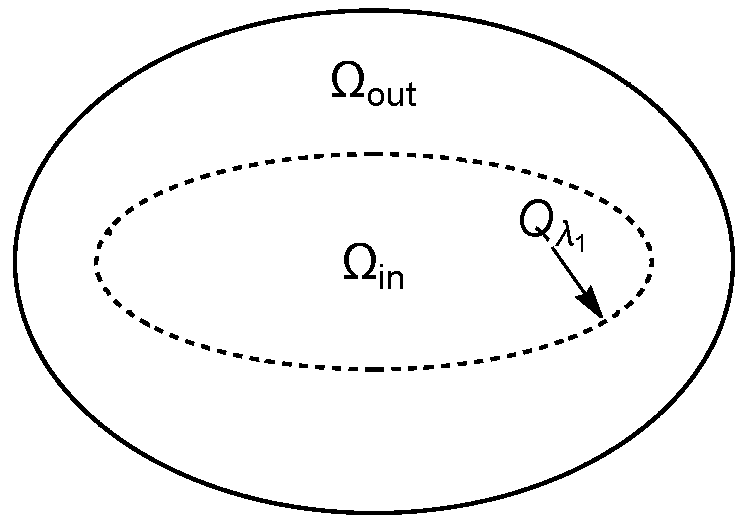
\includegraphics[scale=0.4]{images/ch4/section2/domain_problemA.pdf}
    \caption{Область $\Omega$ для задачи А.}
    \label{fig:pt9:_problemA}
\end{figure}

В области $\Omega = \Omega_{in} \cup \Omega_{out}$ рассмотрим бильярдную систему, подчиняющуюся закону $(\ast)$. В работе \cite{vestnikLatest} показано, что для любой бильярдной траектории ее отрезки, лежащие в области $\Omega_{in}$, касаются одной и той же  софокусной квадрики с параметром $\alpha_{in} \in (\lambda_1, a^2)$, а ее отрезки, лежащие в $\Omega_{out}$ --- вообще говоря, другой квадрики с параметром $\alpha_{out} \in (0, a^2)$. При этом параметры $\alpha_{in}$ и $\alpha_{out}$ связаны соотношением $(\alpha_{out} - \lambda_1) n_{out}^2 = (\alpha_{in} - \lambda_1) n_{in}^2$.

Введем функцию $\Lambda$ положения и скорости материальной точки по формуле 
$\Lambda(x, y, v_x, v_y) =  \dfrac{a^2 v_y^2 + b^2v_x^2 - (x v_y-y v_x)^2}{v_x^2 + v_y^2}$. 
Она имеет смысл коэффициента $\alpha$  софокусной квадрики $Q_\alpha$, которая касается прямой, проходящей через точку $(x,y)$ в направлении вектора $(v_x, v_y)$.
Для классического бильярда в эллипсе эта величина является первым интегралом, не зависящим от полной энергии.

Введем функцию  $\Xi(x, y, v_x, v_y)$ по формуле: 
\begin{equation*}
\Xi(x, y, v_x, v_y) = \left[
\begin{array}{ll}
    \Lambda(x, y, v_x, v_y) n_{in}^2, &  \text{ если } (x,y) \in \Omega_{in} \\
    \Lambda(x, y, v_x, v_y) n_{out}^2 + \lambda_1 (n_{in}^2-n_{out}^2), & \text{ если } (x,y) \in \Omega_{out}    .
\end{array}
\right.
\end{equation*}
Она принимает одно и то же значение на любых отрезках траекторий, лежащих как в $\Omega_{in}$ так и в $\Omega_{out}$. Этот факт следует из равенства $(\alpha_{out} - \lambda_1) n_{out}^2 = (\alpha_{in} - \lambda_1) n_{in}^2$ (см. \cite{vestnikLatest}). 

Задача состоит в том, чтобы для указанной динамической системы описать слоение изоэнергетического трехмерного многообразия  на поверхности уровня первого интеграла $\Xi$.

Рассмотрим плоскость $\mathbb{R}^2$ и отложим по горизонтальной оси величину $\alpha_{in}$ и $\alpha_{out}$ -- по вертикальной оси.
Значению интеграла $\Xi$ поставим в соответствие точку плоскости по формуле
\begin{equation}
\Xi \mapsto \alpha(\Xi) = (\alpha_{in}, \alpha_{out} ) = \left( \frac{\Xi}{n_{in}^2}, \frac{\Xi - \lambda_1 (n_{in}^2 - n_{out}^2)}{n_{out}^2} \right) = \left( \left. \Lambda \right|_{\Omega_{in}}, \left. \Lambda \right|_{\Omega_{out}} \right).
\label{XiToLine}
\end{equation}

Для фиксированных $\lambda_1, n_{in}, n_{out}$ точка $\alpha(\Xi)$ лежит на прямой $L$, которая в декартовых координатах $(\alpha_{in}, \alpha_{out})$ задается уравнением
\begin{equation}
\alpha_{out} = \alpha_{in} \left(\frac{n_{in}}{n_{out}}\right)^2 + \lambda_1 \frac{n_{out}^2 - n_{in}^2}{n_{out}^2}.
\label{eq:L_line}
\end{equation}
Отметим, что прямая $L$ проходит через точку $(\lambda_1, \lambda_1)$ и имеет угловой коэффициент наклона, равный $\frac{n_{in}^2}{n_{out}^2}$. Наглядно можно представлять себе, что возможные случаи соотношений между числами $\lambda_1, n_{in}, n_{out}$ соответствуют всевозможным прямым, проходящим через точку $(\lambda_1, \lambda_1)$ и образующим угол с горизонтальной осью, который меняется от $0$ до  $\frac{\pi}{2}$.

Мы введем структурную диаграмму критических значений первого интеграла $\Xi$. 
Бильярдные траектории могут иметь один из следующих типов, см. рис. \ref{fig:pt9:_causticTypesBulletsDiagram}.
\begin{figure}[!htb]
\minipage{0.45\textwidth}
\centering
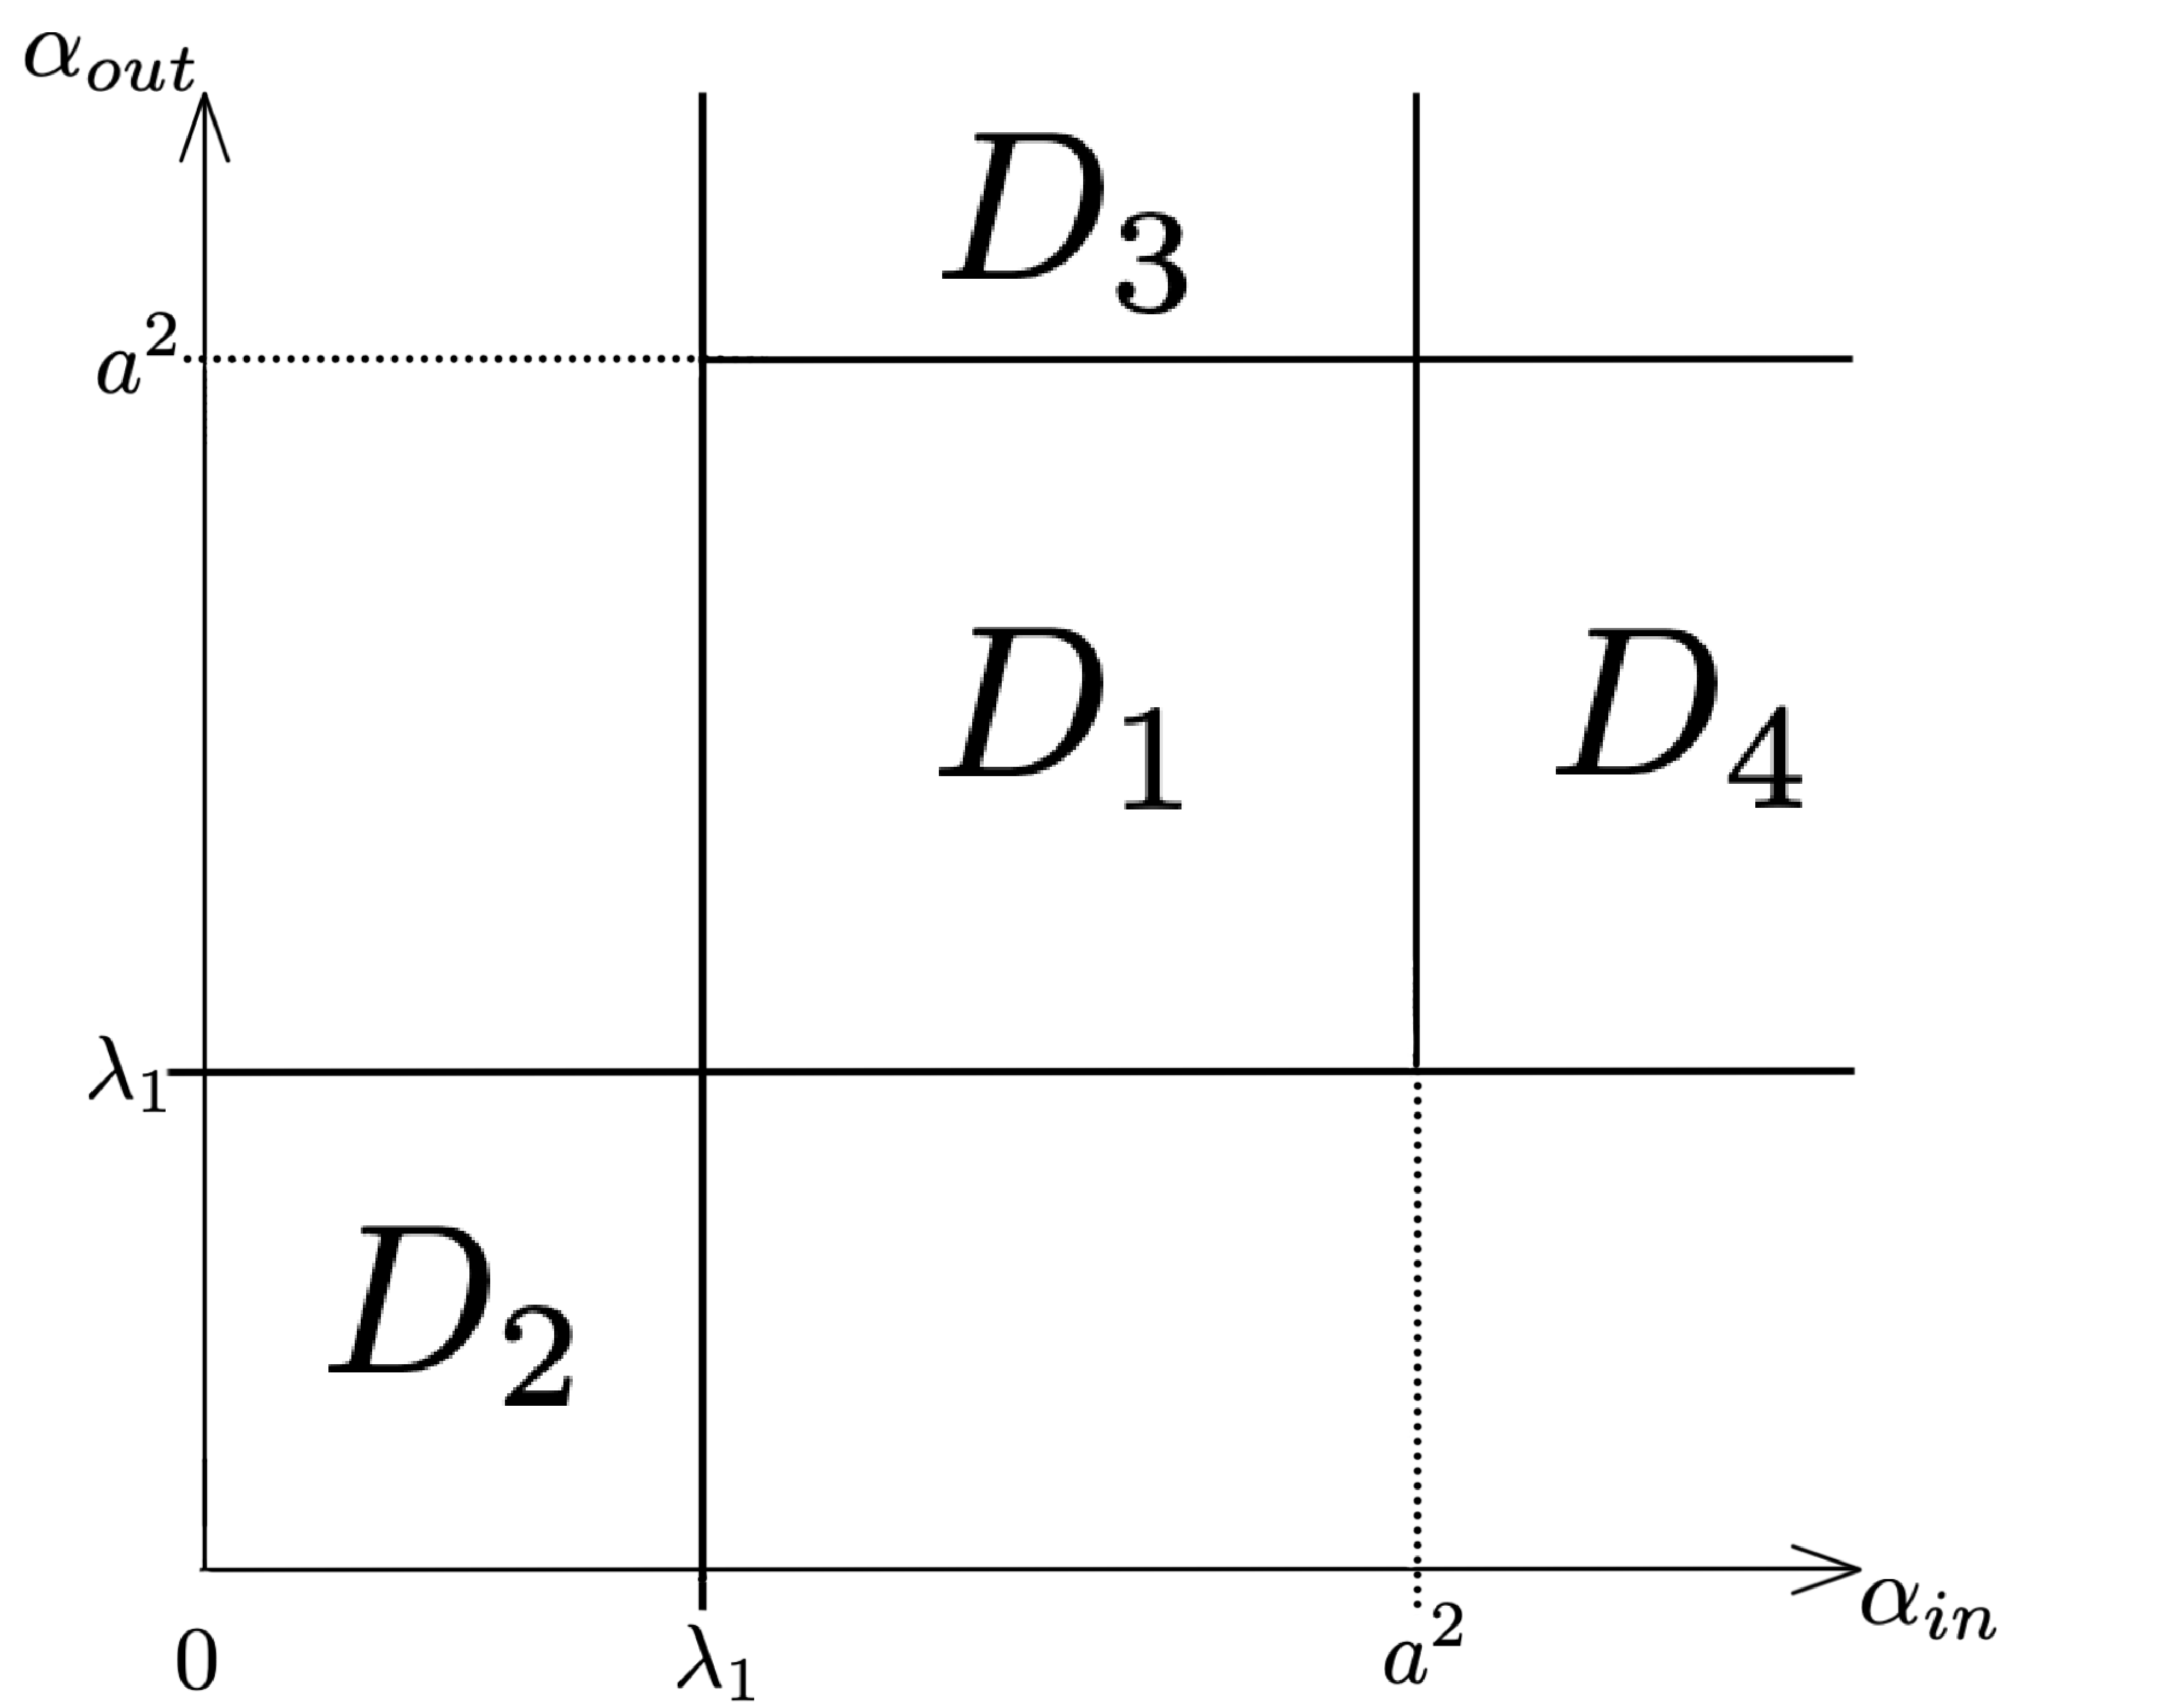
\includegraphics[scale=0.1]{images/ch4/section2/causticTypesBulletsDiagram.pdf}
    \caption{Области возможного движения бильярдной траектории.}
    \label{fig:pt9:_causticTypesBulletsDiagram}
\endminipage\hfill
\minipage{0.55\textwidth}
\centering
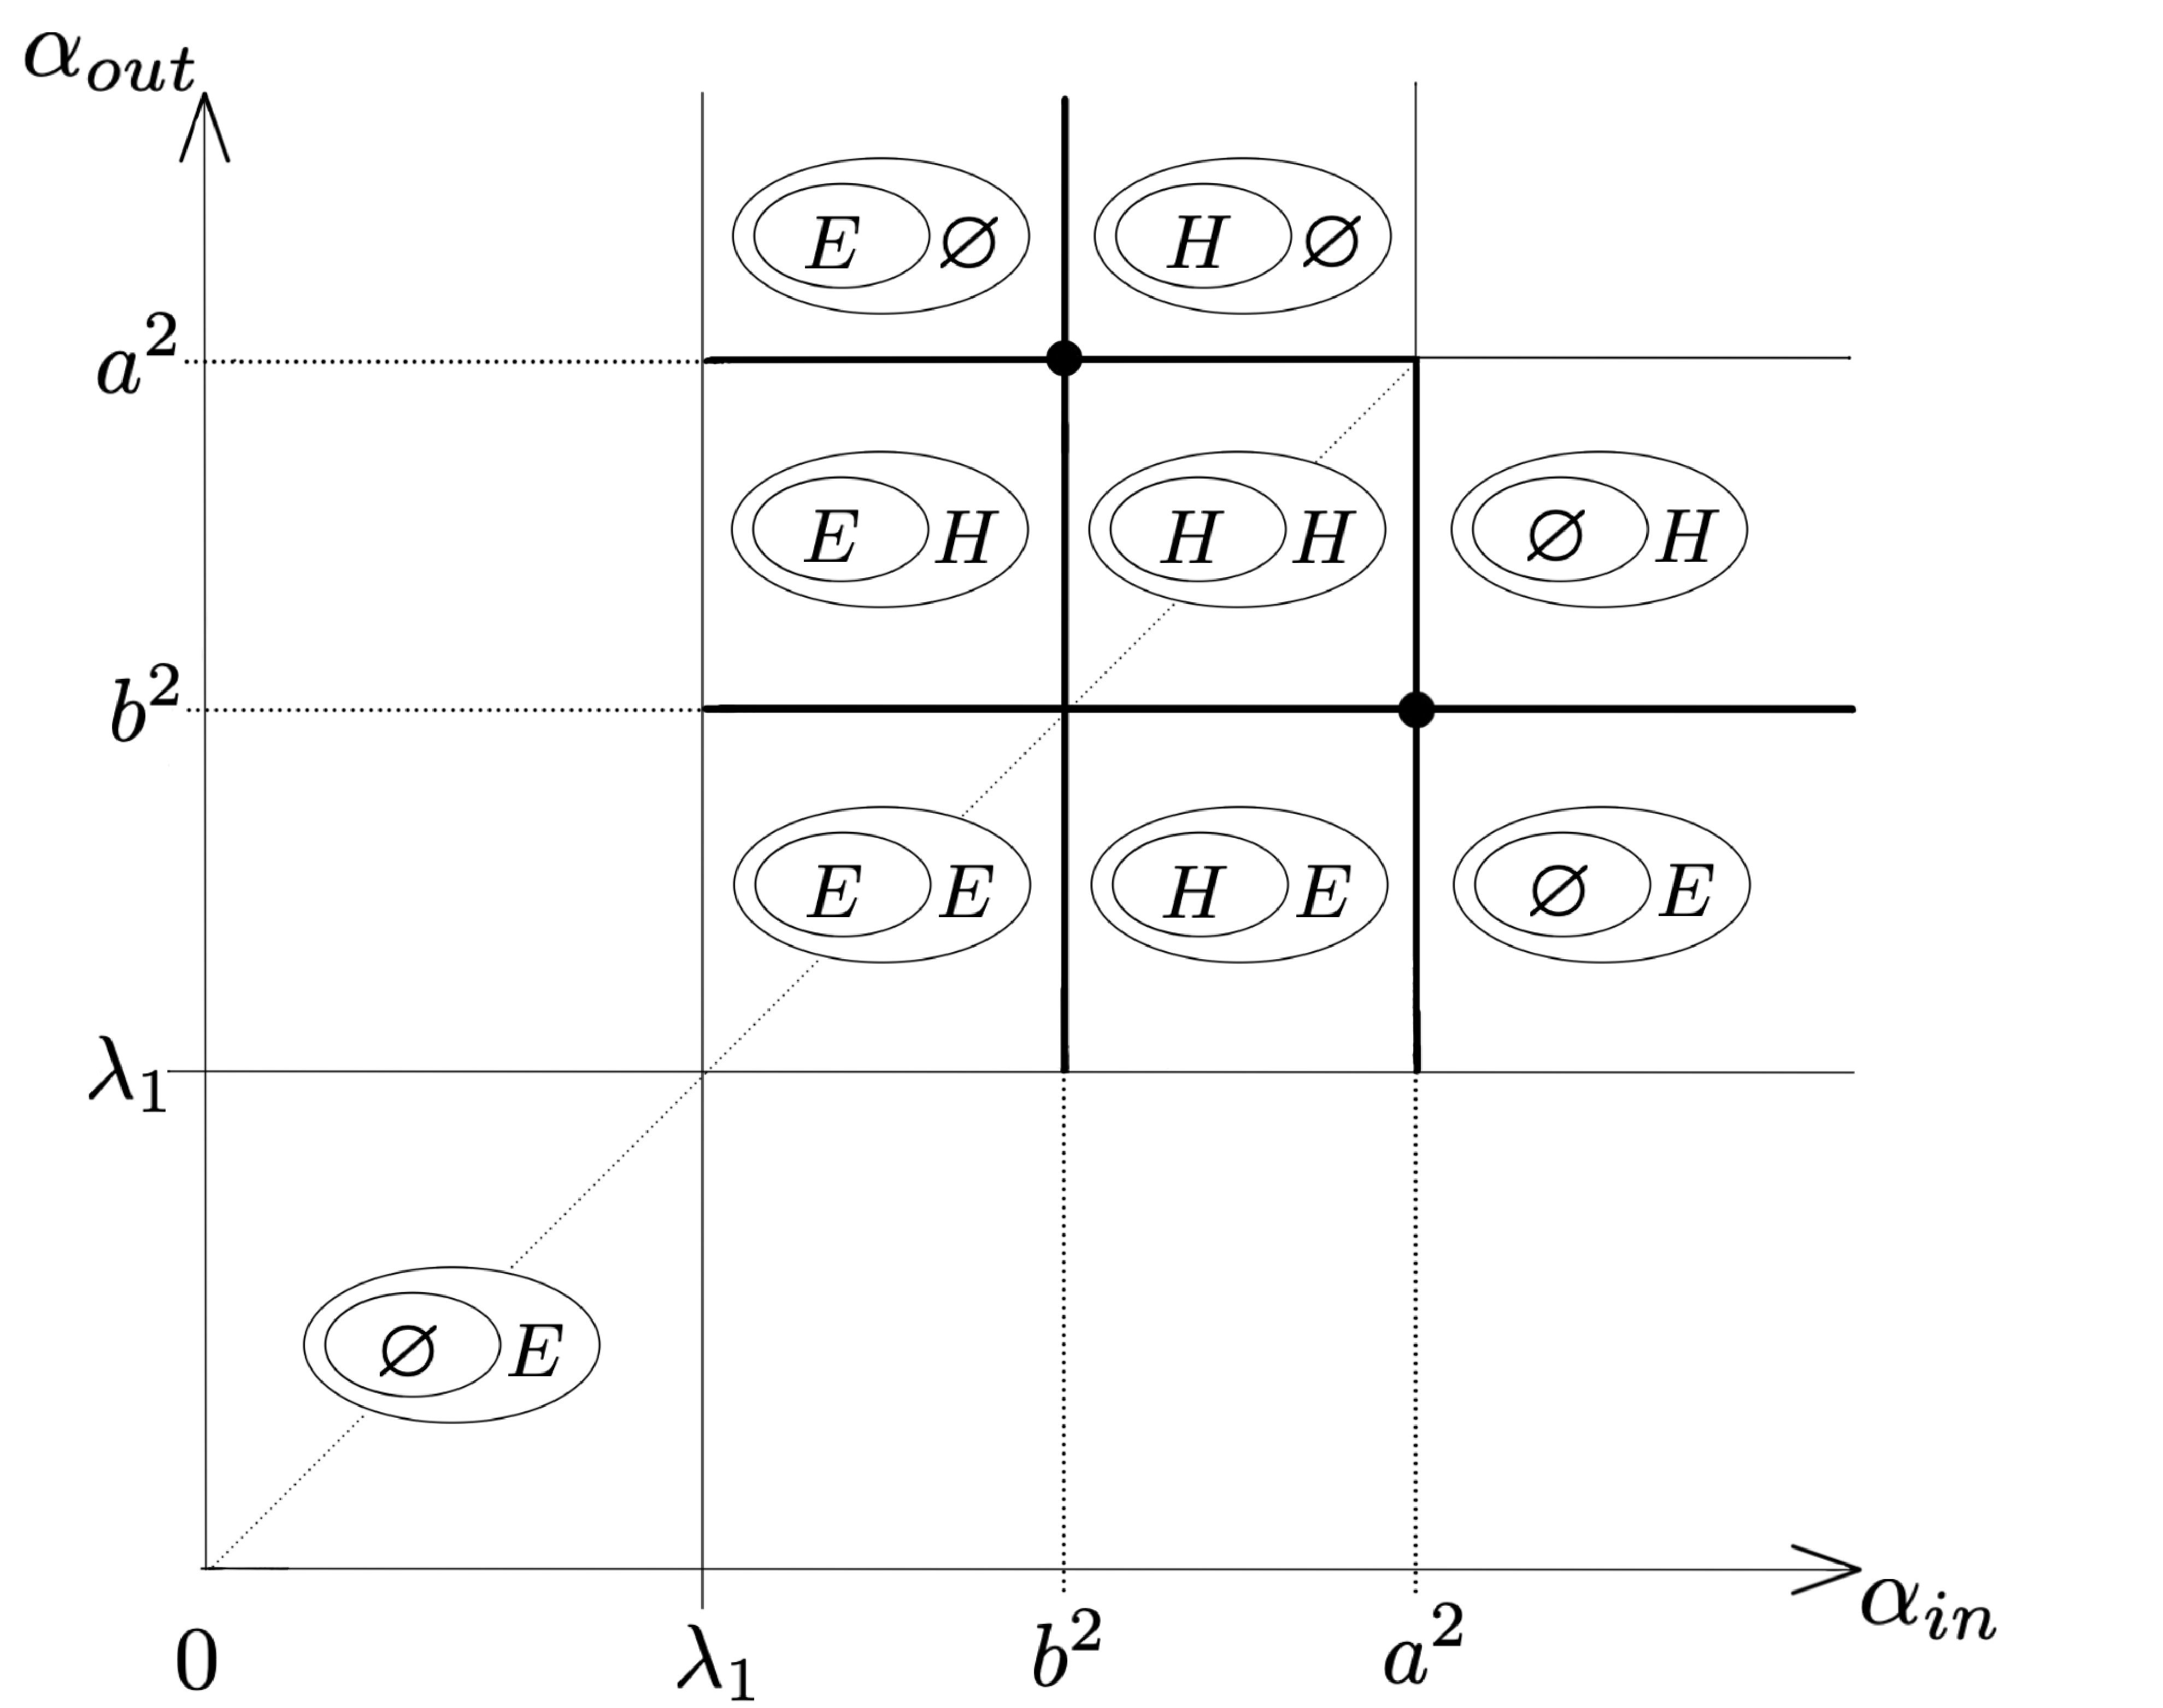
\includegraphics[scale=0.1]{images/ch4/section2/problemAbifurcations.pdf}
    \caption{Возможные типы каустик в $\Omega_{in}$ и $\Omega_{out}$. Жирным выделены особые значения для $\alpha_{in}$, $\alpha_{out}$. См. также замечание \ref{rem:remark1}.}
    \label{fig:pt9:_problemAbifurcations}
\endminipage\hfill
\end{figure}

$D1:$ Сначала рассмотрим траекторию, которая заходит в каждую из областей $\Omega_{in}$ и $\Omega_{out}$.
Будем обозначать через $\alpha_{in}$ и $\alpha_{out}$ параметры квадрик, которых касаются отрезки траектории бильярда, находящиеся в областях $\Omega_{in}$ и $\Omega_{out}$, соответственно. В этом случае  $\alpha_{in} \in (\lambda_1, a^2)$, $\alpha_{out} \in (0, a^2)$.

$D2:$ Возможна траектория, целиком находящаяся в области $\Omega_{out}$ и имеющая каустикой эллипс. В этом случае параметр $\alpha_{in}$ не определен, а $\alpha_{out}$ лежит в интервале $\alpha_{out} \in (0, \lambda_1)$.

$D3:$ В случае, если траектория целиком содержится в $\Omega_{in}$, параметр $\alpha_{out}$ не определен. При этом если траектория имеет каустикой эллипс, то $\alpha_{in}$ лежит в интервале $(\lambda_1, b^2)$, а если гиперболу --- в интервале $(b^2, a^2)$.
 Такие траектории испытывают полное внутреннее отражение на границе областей $\Omega_{in}, \Omega_{out}$ и возникают при определенных соотношениях между параметрами $n_{in}, n_{out}$. 

$D4:$ Для траекторий, целиком находящихся в области $\Omega_{out}$ и имеющих каустикой гиперболу,  параметр $\alpha_{in}$ также не определен, а $\alpha_{out}$ лежит в интервале $(b^2, a^2)$.
Такие траектории также испытывают полное внутреннее отражение на границе областей $\Omega_{in}, \Omega_{out}$ и возникают при определенных соотношениях между параметрами $n_{in}, n_{out}$.


Анализ слоения на поверхности уровня интеграла $\Xi$ проходит по следующей схеме.
Сначала фиксируются параметры $\lambda_1, n_{in}, n_{out}$. Они определяют прямую $L$, при этом значение интеграла $\Xi$ однозначно определяет точку на этой прямой. Структура слоения определяется тем, как прямая $L$ пересекает области $D_1, D_2, D_3, D_4$.
Пересечение прямой $L$ с областью $D_1$ определяет значения $\Xi$, при которых имеет место движение типа $D_1$; определены оба параметра $\alpha_{in}, \alpha_{out}$.
Пересечение этой прямой с областью $D_2$ определяет движение типа $D_2$, и при этом  параметр $\alpha_{in}$ не имеет смысла; для $D_3$ аналогично. 
Пересечение прямой с областью $D_4$ определяет движение типа $D_4$, в этом случае не  определен параметр $\alpha_{out}$.

%Это соотношение имеет смысл рассматривать для случая $D_1$. Для случаев $D_2$ и $D_3$ параметр $\alpha_{in}$ не определен. Для случая $D_4$ не определен параметр $\alpha_{out}$. Для фиксированных значений $n_{in}, n_{out}, \lambda_1$ соответствие $\Xi \mapsto \alpha(\Xi)$
%\begin{remark} 
%Заметим, что при $0 < \alpha_{out} < \lambda_1$ траектория бильярда целиком находится в $\Omega_{out}$ и не попадает в область $\Omega_{in}$. 
%Следовательно, параметр $\alpha_{in}$ в этом случае не определен.
%Поэтому принадлежность интеграла $\Xi$ этой прямой в квадрате $0 < \alpha_{in}, \alpha_{out} < \lambda_1$ и в областях $\alpha_{in}, \alpha_{out} > a^2$ весьма условная. Мы не будем заострять на этом внимание в угоду наглядности диаграммы \ref{fig:pt9:_causticTypesDiagram}.
%\end{remark}

%(0, \lambda_1 \left(1 - \frac{n_{in}^2}{n_{out}^2}\right) )$. Интеграл $\Xi$ соответствует некоторой точке на этой прямой. 


При этом нерегулярные значения интеграла $\Xi$ соответствуют точкам пересечения  прямой $L$ с координатными линиями $\alpha_{in},\alpha_{out} = b^2, a^2$, изображенным жирными линиями на рис. \ref{fig:pt9:_problemAbifurcations}.
Особый интерес вызывают случаи, когда $L$ проходит через точку $(\alpha_{in}, \alpha_{out}) = (a^2, b^2)$ или точку  $(\alpha_{in}, \alpha_{out}) = (b^2, a^2)$.
\begin{remark}
В случае, когда совпадают коэффициенты $n_{in}$ и $n_{out}$, траектории проходят из $\Omega_{in}$ в $\Omega_{out}$ и обратно без преломления, тем самым мы получаем динамику классического бильярда в эллипсе. Этому соответствует прямая $L$, проходящая по пунктирной диагонали на рис. \ref{fig:pt9:_problemAbifurcations}.

На рис. \ref{fig:pt9:_problemAbifurcations} схематично показаны типы каустик в областях $\Omega_{in}$ и $\Omega_{out}$:  $H$ означает, что каустика является гиперболой, $E$ соответствует эллипсу, а $\varnothing$ означает, что траектория не заходит внутрь соответствующей области. 
\label{rem:remark1}
\end{remark}
%Для удобства занумеруем регулярные области значений интеграла $\Xi$ на рис. \ref{fig:pt9:_causticTypesDiagram}.
%В ходе их описания мы узнаем как выглядят соответствующие области $\Omega$. Потом, когда будем описывать бифуркации, 

Параметры  $\alpha_{in}$, $\alpha_{out}$ имеют критические значения $b^2, a^2$. Соответствующие вертикальные и горизонтальные прямые, а также диагональ $\alpha_{in} = \alpha_{out}$, разбивают области $D_1, \ldots, D_4$ на подобласти, показанные на рис. \ref{fig:pt9:_problemA_subdivisions}. Формально эти подобласти определены в теореме \ref{st:pt9:n1_n2_surfaces}.
\begin{figure}[!htb]
\centering
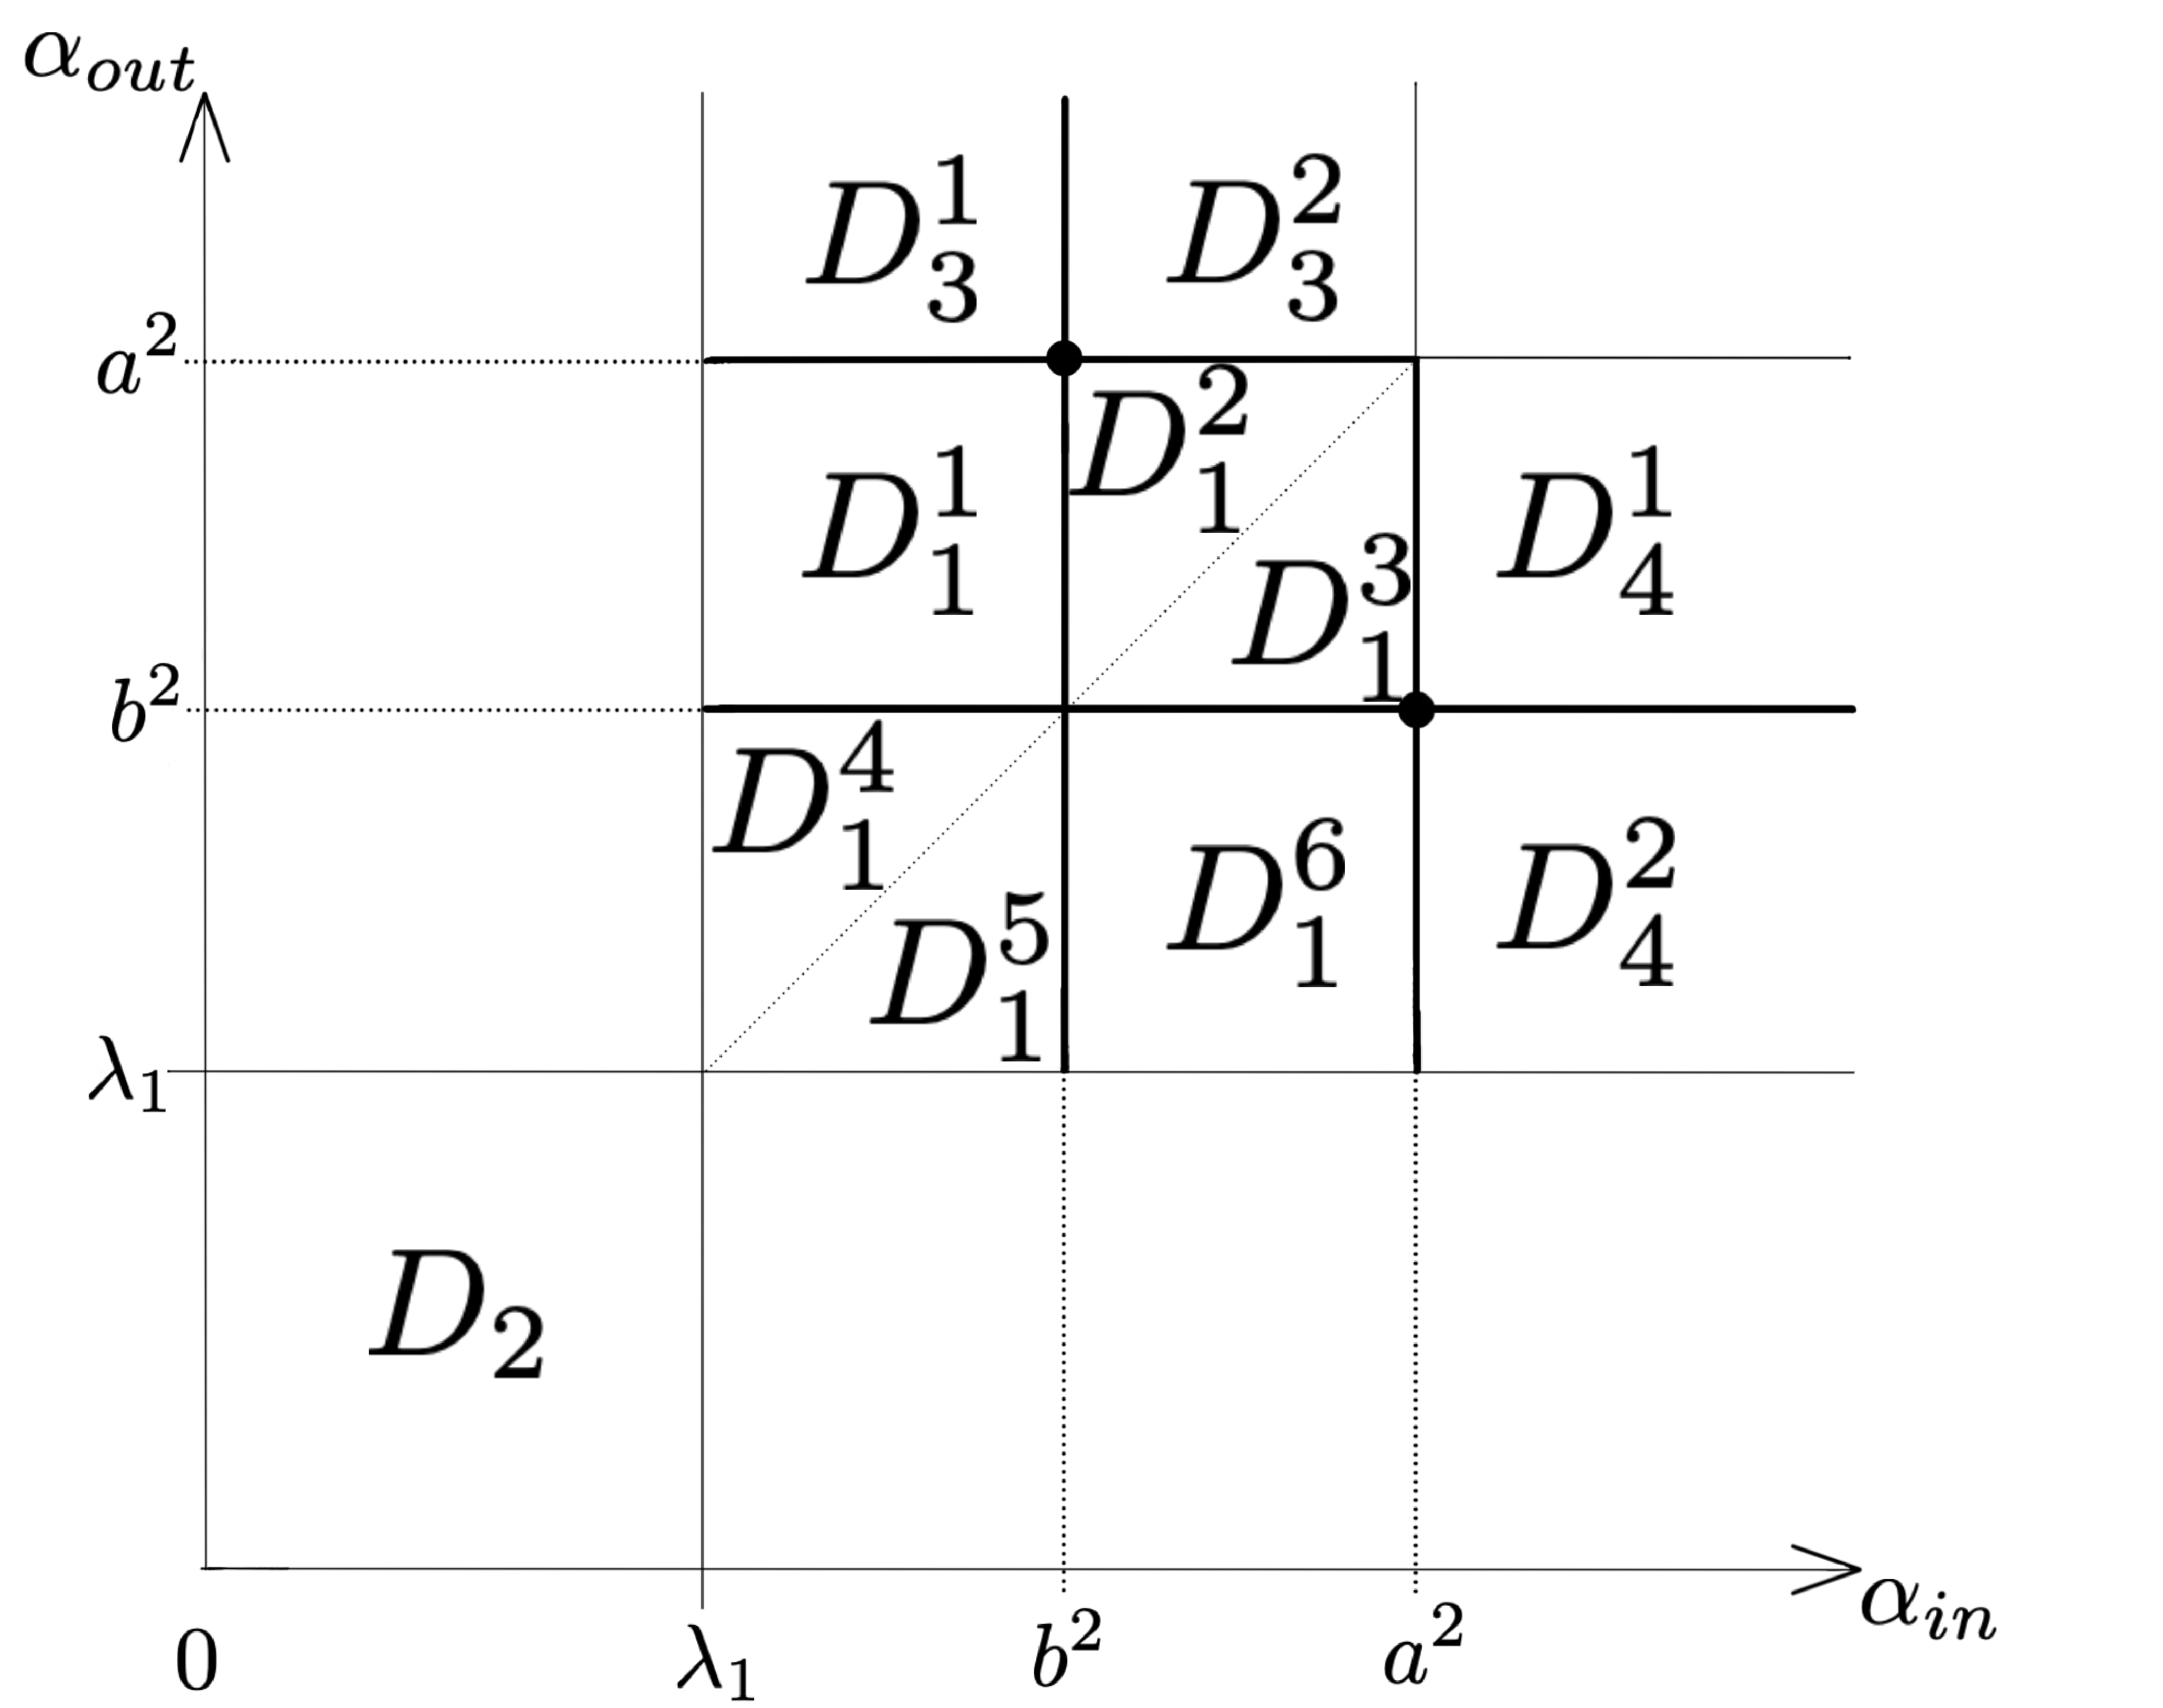
\includegraphics[scale=0.1]{images/ch4/section2/problemA_subdivisions.pdf}
    \caption{Подразбиение областей $D_1, \ldots, D_4$.}
    \label{fig:pt9:_problemA_subdivisions}
\end{figure}

\subsection{Поверхности уровня для регулярных значений интеграла $\Xi$}
\begin{theorem} 
Областям $D_i^j$ в плоскости $(\alpha_{in}, \alpha_{out})$ соответствуют следующие поверхности $\Xi = \const$
\medskip
\begin{center}
\begin{tabular}{|c|c|c|}
\hline 
$D_1^1$  	& 	$\alpha_{in} \in (\lambda_1, b^2), \ \alpha_{out} \in (b^2, a^2)$			& сфера с 5 ручками; \\ \hline 
$D_1^2$  	& 	$\alpha_{in} \in (b^2, a^2), \ \alpha_{out} \in (\alpha_{in}, a^2)$				& сфера с 5 ручками; \\ \hline 
$D_1^3$  	& 	$\alpha_{in} \in (b^2, a^2), \ \alpha_{out} \in (b^2, \alpha_{in})$				& сфера с 5 ручками; \\ \hline 
$D_1^4$ 	& 	$\alpha_{in} \in (\lambda_1, b^2), \ \alpha_{out} \in (\alpha_{in}, b^2)$	& 2 дизъюнктных тора; \\ \hline 
$D_1^5$  	& 	$\alpha_{in} \in (\lambda_1, b^2), \ \alpha_{out} \in (\lambda_1, \alpha_{in})$	& 2 дизъюнктных тора; \\ \hline 
$D_1^6$  	& 	$\alpha_{in} \in (b^2, a^2), \ \alpha_{out} \in (\lambda_1, b^2)$			& сфера с 5 ручками; \\ \hline 
\hline
$D_2$  	& 	$(\alpha_{out} \in (0, \lambda_1), \ \alpha_{in} < \lambda_1)$ или & \\
		&  $(\alpha_{in} \in (0, \lambda_1), \ \alpha_{out} < \lambda_1)$				& 2 дизъюнктных тора; \\ \hline
 \hline
$D_3^1$  	& 	$\alpha_{in} \in (\lambda_1, b^2), \ \alpha_{out} > a^2$				& 2 дизъюнктных тора; \\ \hline 
$D_3^2$  	& 	$\alpha_{in} \in (b^2, a^2), \ \alpha_{out} > a^2 $					& 1 тор; \\ \hline 
\hline 
$D_4^1$  	& 	$\alpha_{in} > a^2, \ \alpha_{out} \in (b^2, a^2)$						& 2 дизъюнктных тора; \\ \hline 
$D_4^2$  	& 	$\alpha_{in} > a^2, \alpha_{out} \in (\lambda_1, b^2)$				& 2 дизъюнктных тора; \\ \hline 
\end{tabular}
\end{center}
%\[
%\begin{array}{c|c|c}
%D_2  & & \text{2 дизъюнктных тора}; \\
%
%
%\alpha_{out} \in (\lambda_1, b^2) & \alpha_{in} \in (\lambda_1, b^2) &  \text{2 дизъюнктных тора}; \\
% & \alpha_{in} \in (b^2, a^2) &  \text{сфера с 5 ручками}; \\
% & \alpha_{in} > a^2 &   \text{2 дизъюнктных тора}; \\
%
%\alpha_{out} \in (b^2, a^2)  & \alpha_{in} \in (\lambda_1, b^2) &  \text{сфера с 5 ручками}; \\
% & \alpha_{in} \in (b^2, a^2), \ \alpha_{in} \neq \alpha_{out} &  \text{сфера с 5 ручками}; \\
%  & \alpha_{in} \in (b^2, a^2), \ \alpha_{in} = \alpha_{out} &  \text{тор}; \\
% & \alpha_{in}  > a^2 &   \text{2 дизъюнктных тора}; \\
%
%\alpha_{out} > a^2 & \alpha_{in} \in (\lambda_1, b^2) &  \text{2 дизъюнктных тора}; \\
% & \alpha_{in} \in (b^2, a^2) &  \text{1 тор}. \\
%\end{array}
%\]
\label{st:pt9:n1_n2_surfaces}
\end{theorem} 



\begin{proof}

%Доказательство будет основываться на соображениях, предложенных в \cite[\S 3]{Fok15}.

\textbf{Случай $D_1^4$, $D_1^5$.}
%Касательные к траекториям бильярда в области $\Omega_{out}$ будут касаться некоторого эллипса с параметром $\alpha_{out}$. В области $\Omega_{in}$ параметром такого эллипса выступает $\alpha_{in}$. 
Продолжения звеньев траектории, лежащих в $\Omega_{out}$, касаются каустики с параметром $\alpha_{out}$, а звенья траектории в области $\Omega_{in}$ касаются каустики с параметром $\alpha_{in}$. При этом оба параметра $\alpha_{in}, \alpha_{out}$ находятся в интервале $(\lambda_1, b^2)$, то есть обе каустики являются эллипсами.

Спроектируем точку траектории $(x,y,v_x, v_y)$ на бильярдную область:
$$\pi : (x,y,v_x, v_y) \mapsto (x, y).$$
Рассмотрим всевозможные траектории с фиксированным значением $\Xi$, относящимся к случаям $D_1^4, D_1^5$. Тогда проекция $(x,y) \in \Omega_{out}$ заметает всю область $\Omega_{out}$, а проекция  $(x,y) \in \Omega_{in}$ заметает кольцо $\widetilde{\Omega}_{in} = \Omega_{in} \setminus \text{ int }(\Omega_{\alpha_{in}})$, где $\Omega_{\alpha_{in}}$ --- это область, ограниченная квадрикой $Q_{\alpha_{in}}$. 

Поверхность $\Xi = \const$ склеена из нескольких копий $\widetilde{\Omega}_{in}$ и $\Omega_{out}$. 

Во всех внутренних точках $\widetilde{\Omega}_{in}$ и $\Omega_{out}$ проекция $(x, y, v_x, v_y) \mapsto (x,y)$ четырехлистная.
В прообразе этой проекции на поверхности $\Xi = \const$ выберем по 4 прообраза для областей $\Omega_{out}$ и $\widetilde{\Omega}_{in}$, обозначим эти прообразы 
$\Omega_{out, j}$ и $\Omega_{in, j}$, $j=1,\ldots,4$, 
где нумерация определена по следующему правилу:

\begin{equation}
\begin{array}{ll}
1: & \text{ вектор } (v_x, v_y) \text{ направлен по часовой стрелке к эллипсу } Q_{\alpha}, \\
2: & \text{ вектор } (v_x, v_y) \text{ направлен против часовой стрелки к эллипсу }  Q_{\alpha}, \\
3: & \text{ вектор } (v_x, v_y) \text{ направлен против часовой стрелки от эллипса }  Q_{\alpha}, \\
4: & \text{ вектор } (v_x, v_y) \text{ направлен по часовой стрелке от эллипса }  Q_{\alpha},
\end{array}
\label{eq:ell_numeration}
\end{equation}
где $\alpha$ --- параметр каустики, т.е. $\alpha=\alpha_{out}$ для $(x,y) \in \Omega_{out}$ и $\alpha=\alpha_{in}$ для $(x,y) \in \widetilde{\Omega}_{in}$.

Поверхность $\Xi=\const$ в рассматриваемом случае склеена из 8 эллиптических колец $\Omega_{out, j}, \Omega_{in, j}, \ j=1, \ldots, 4$. 
Проследим правила склейки:

$\bullet$ $\Omega_{out, j}$ и $\Omega_{in, j}$ отождествляются по общей границе, которая проектируется в $Q_{\lambda_1}$, поскольку правила $(\ast)$ сохраняют номер в случае, когда обе каустики являются эллипсами.
Получим 4 области, которые обозначим как $\widetilde{\Omega}_1, \widetilde{\Omega}_2, \widetilde{\Omega}_3, \widetilde{\Omega}_4$, где $\widetilde{\Omega}_j = \Omega_{out, j} \cup \widetilde{\Omega}_{in, j}, \ j=1, \ldots, 4$.

$\bullet$ На внешней границе $\widetilde{\Omega}_1$ приклеивается к $\widetilde{\Omega}_4$, а $\widetilde{\Omega}_2$ к $\widetilde{\Omega}_3$ в силу стандартного закона отражения.

$\bullet$ На внутренней границе $\widetilde{\Omega}_1$ подклеивается к $\widetilde{\Omega}_4$, а $\widetilde{\Omega}_2$ подклеивается к $\widetilde{\Omega}_3$ в силу смены номера листа после касания звеном траектории каустики $Q_{\alpha_{in}}$.

%\textcolor{red}{старое}
%Рассмотрим область, которая целиком содержит траекторию бильярда, то есть область 
%$\widetilde{\Omega} = \Omega_{out} \cup \widetilde{\Omega}_{in} = \Omega_{out} \cup (\Omega_{in} \setminus \text{ int } Q_{\alpha_{in}})$, 
%где из $\Omega_{in}$ мы вырезаем внутренность эллипса с параметром $\alpha_{in}$. 
%
%В произвольной внутренней точке $\widetilde{\Omega}$, исключая $Q_{\lambda_1}$,  определены 4 вектора скорости $(v_x, v_y)$ таких, что $(x, y, v_x, v_y)$ лежит на соответствующем уровне интеграла $\Xi$. 
%А именно, векторы принадлежат касательной к каустике $Q_{\alpha_{in}}$ для $(x, y) \in \Omega_{in}$ или к каустике $Q_{\alpha_{out}}$ для $(x, y) \in \Omega_{out}$.
%
%Здесь и далее считаем, что точкам $(x, y) \in \Omega_{in}$ соответствуют векторы $v_i, i=1,\ldots,4$, а точкам $(x, y) \in \Omega_{out}$ --- векторы $w_i, i=1,\ldots,4$.
%Нумерацию векторов для эллиптической каустики установим следующую (см. рис. \ref{fig:pt9:_caseD14}):
%
%\begin{figure}[!htb]
%\centering
%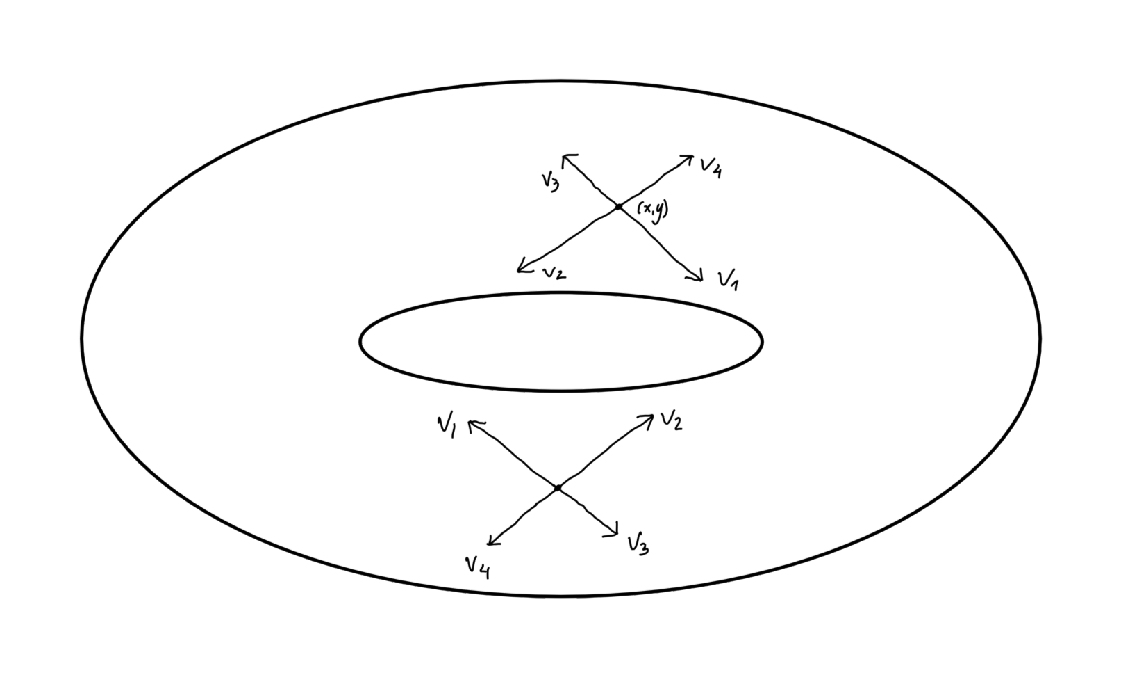
\includegraphics[scale=0.45]{images/ch4/section2/caseD14.pdf}
%    \caption{Определение векторов скорости в случае эллиптической каустики.}
%    \label{fig:pt9:_caseD14}
%\end{figure}
%
%\begin{remark}
%Пусть $\alpha$ --- параметр эллиптической каустики, точка $(x,y)$ находится вне эллипса $Q_{\alpha}$, а векторы $\nu_i$ задают касательную к нему, проходящую через $(x,y)$. Тогда нумерацию определим следующим образом:
%\begin{equation}
%\begin{array}{ll}
%\nu_1, & \text{ --  направлен по часовой стрелке к эллипсу } Q_{\alpha}, \\
%\nu_2, & \text{ --  направлен против часовой стрелки к эллипсу }  Q_{\alpha}, \\
%\nu_3, & \text{ --  направлен против часовой стрелки от эллипса }  Q_{\alpha}, \\
%\nu_4, & \text{ --  направлен по часовой стрелке от эллипса }  Q_{\alpha}.
%\end{array}
%\end{equation}
%\label{eq:vectors_roles}
%\end{remark}
%
%Так определим векторы $v_i, \ i=1, \ldots, 4$ для точек $(x,y) \in \widetilde{\Omega}_{in}$.
%Векторы $w_i, \ i=1,\ldots, 4$ для точек $(x,y) \in \widetilde{\Omega}_{out}$ определяются аналогично с точностью до замены эллипса $Q_{\alpha_{in}}$ на $Q_{\alpha_{out}}$.
%
%При этом точки $(x, y) \in Q_{\lambda_1}$ являются граничными для $\Omega_{out}$ и $\Omega_{in}$.
%В этих точках соответствие между векторами $v_i$ и $w_j$ устанавливается исходя из закона преломления $(\ast)$. 
%
%
%Под листом $\Sigma_{i, out}$ будем понимать пару $(\Omega_{out}, w_i)$. Аналогично 
%лист $\Sigma_{j, in}$ обозначает пару $(\widetilde{\Omega}_{in}, v_j)$. 
%%Листы будем подклеивать друг к другу 
%В разбираемом случае на эллипсе с параметром $\lambda_1$ закон преломления влечет \textit{правило склейки} $\Sigma_{i, out} \sim \Sigma_{i, in}$. 
%Для краткости  можем определить большой лист $\Sigma_k$, соответствующий склейке $\Sigma_{k, out} \cup \Sigma_{k, in}$.
%%Здесь и далее это правило склейки $\Omega_{out}$ с $\widetilde{\Omega}_{in}$ используем без явного упоминания соответствия.
%%Очевидно, что такое соответствие локально является непрерывным. 
%
%На дугах внешнего граничного эллипса $Q_0$ закон отражения приводит к слейкам областей $\Sigma_1 \sim \Sigma_4$ и $\Sigma_2 \sim \Sigma_3$. 
%При интегральном эллипсе $Q_{\alpha_{in}}$ в силу тождественного совпадения $v_1 = v_4$ и $v_2 = v_3$ возникают склейки $\Sigma_1 \sim \Sigma_4$ и $\Sigma_2 \sim \Sigma_3$.
Таким образом, для случая  $D_1^4$, $D_1^5$ поверхности уровня интеграла $\Xi$ являются  несвязным объединением двух торов.

%\marginpar{мы устали}
\medskip
\textbf{Случай $D_2$.} 
Траектория целиком содержится в $\Omega_{out}$. Точки проекции $(x,y)$ заметают $\widetilde{\Omega} = \Omega_{out} \setminus \Omega_{\alpha_{out}}$, при этом проекция четырехлистная, как и в предыдущем случае. 
Четыре прообраза $\widetilde{\Omega}$ нумеруются по правилам, указанным в предыдущем случае. 
Внешние и внутренние границы $\widetilde{\Omega}_1$ подклеиваются к соответствующим границам $\widetilde{\Omega}_4$, аналогично для $\widetilde{\Omega}_2$ и $\widetilde{\Omega}_3$. Результатом склейки являются два дизъюнктных тора.
%Повторяя соображения предыдущего случая, на граничном и интегральном торах возникают склейки $\Sigma_1 \sim \Sigma_4$ и $\Sigma_2 \sim \Sigma_3$. Результатом склейки также выступают два тора.

\medskip
\textbf{Случай $D_4^2$. } Траектория снова целиком содержится в $\Omega_{out}$ и отражается от обеих границ внешнего кольца. Рассуждения, аналогичные случаю $D_2$ с той лишь разницей, что вместо $\alpha_{out}$ пишется $\lambda_1$, а вместо касания на внутренней границе используется отражение, показывают, что в этом случае поверхностью уровня $\Xi=\const$ являются два дизъюнктных тора.

\medskip
\textbf{Случай $D_3^1$. } аналогичен случаю $D_4^2$ с той лишь разницей, что траектория целиком содержится в $\Omega_{in}$. Более точно, в кольце между эллипсами $Q_{\lambda_1}$ и $Q_{\alpha_{in}}$. Поверхностью уровня снова служат два тора.

%Остаются еще 2 случая, в которых одна из каустик является эллипсом. При этом вторая будет гиперболой.
%Рассмотрение гиперболических каустик начнем со случая $D_3^2$.

\medskip
\textbf{Случай $D_3^2$.}
Траектория целиком содержится в $\Omega_{in}$, при этом касается ветвей гиперболы с параметром $\alpha_{in}$ и отражается от внешней границы эллипса $\Omega_{in}$.

По аналогии с предыдущими случаями определим $\widetilde{\Omega}$ как часть внутренности области $\Omega_{in}$, лежащую между ветвей гиперболы $Q_{\alpha_{in}}$ (см. рис. \ref{fig:pt9:_hyp_domain_example}). При проекции $\pi$ прообразом области  $\widetilde{\Omega}$ служат 4 листа $\widetilde{\Omega}_{j}, i=1, \ldots, 4$. Нумерацию листов см. рис. \ref{fig:pt9:_hyp_vectors_numbering}. Сплошным изображены те векторы $(v_x, v_y)$ которые направлены в сторону точки касания звена траектории с каустикой.

\begin{figure}[!htb]
\minipage{0.45\textwidth}
\centering
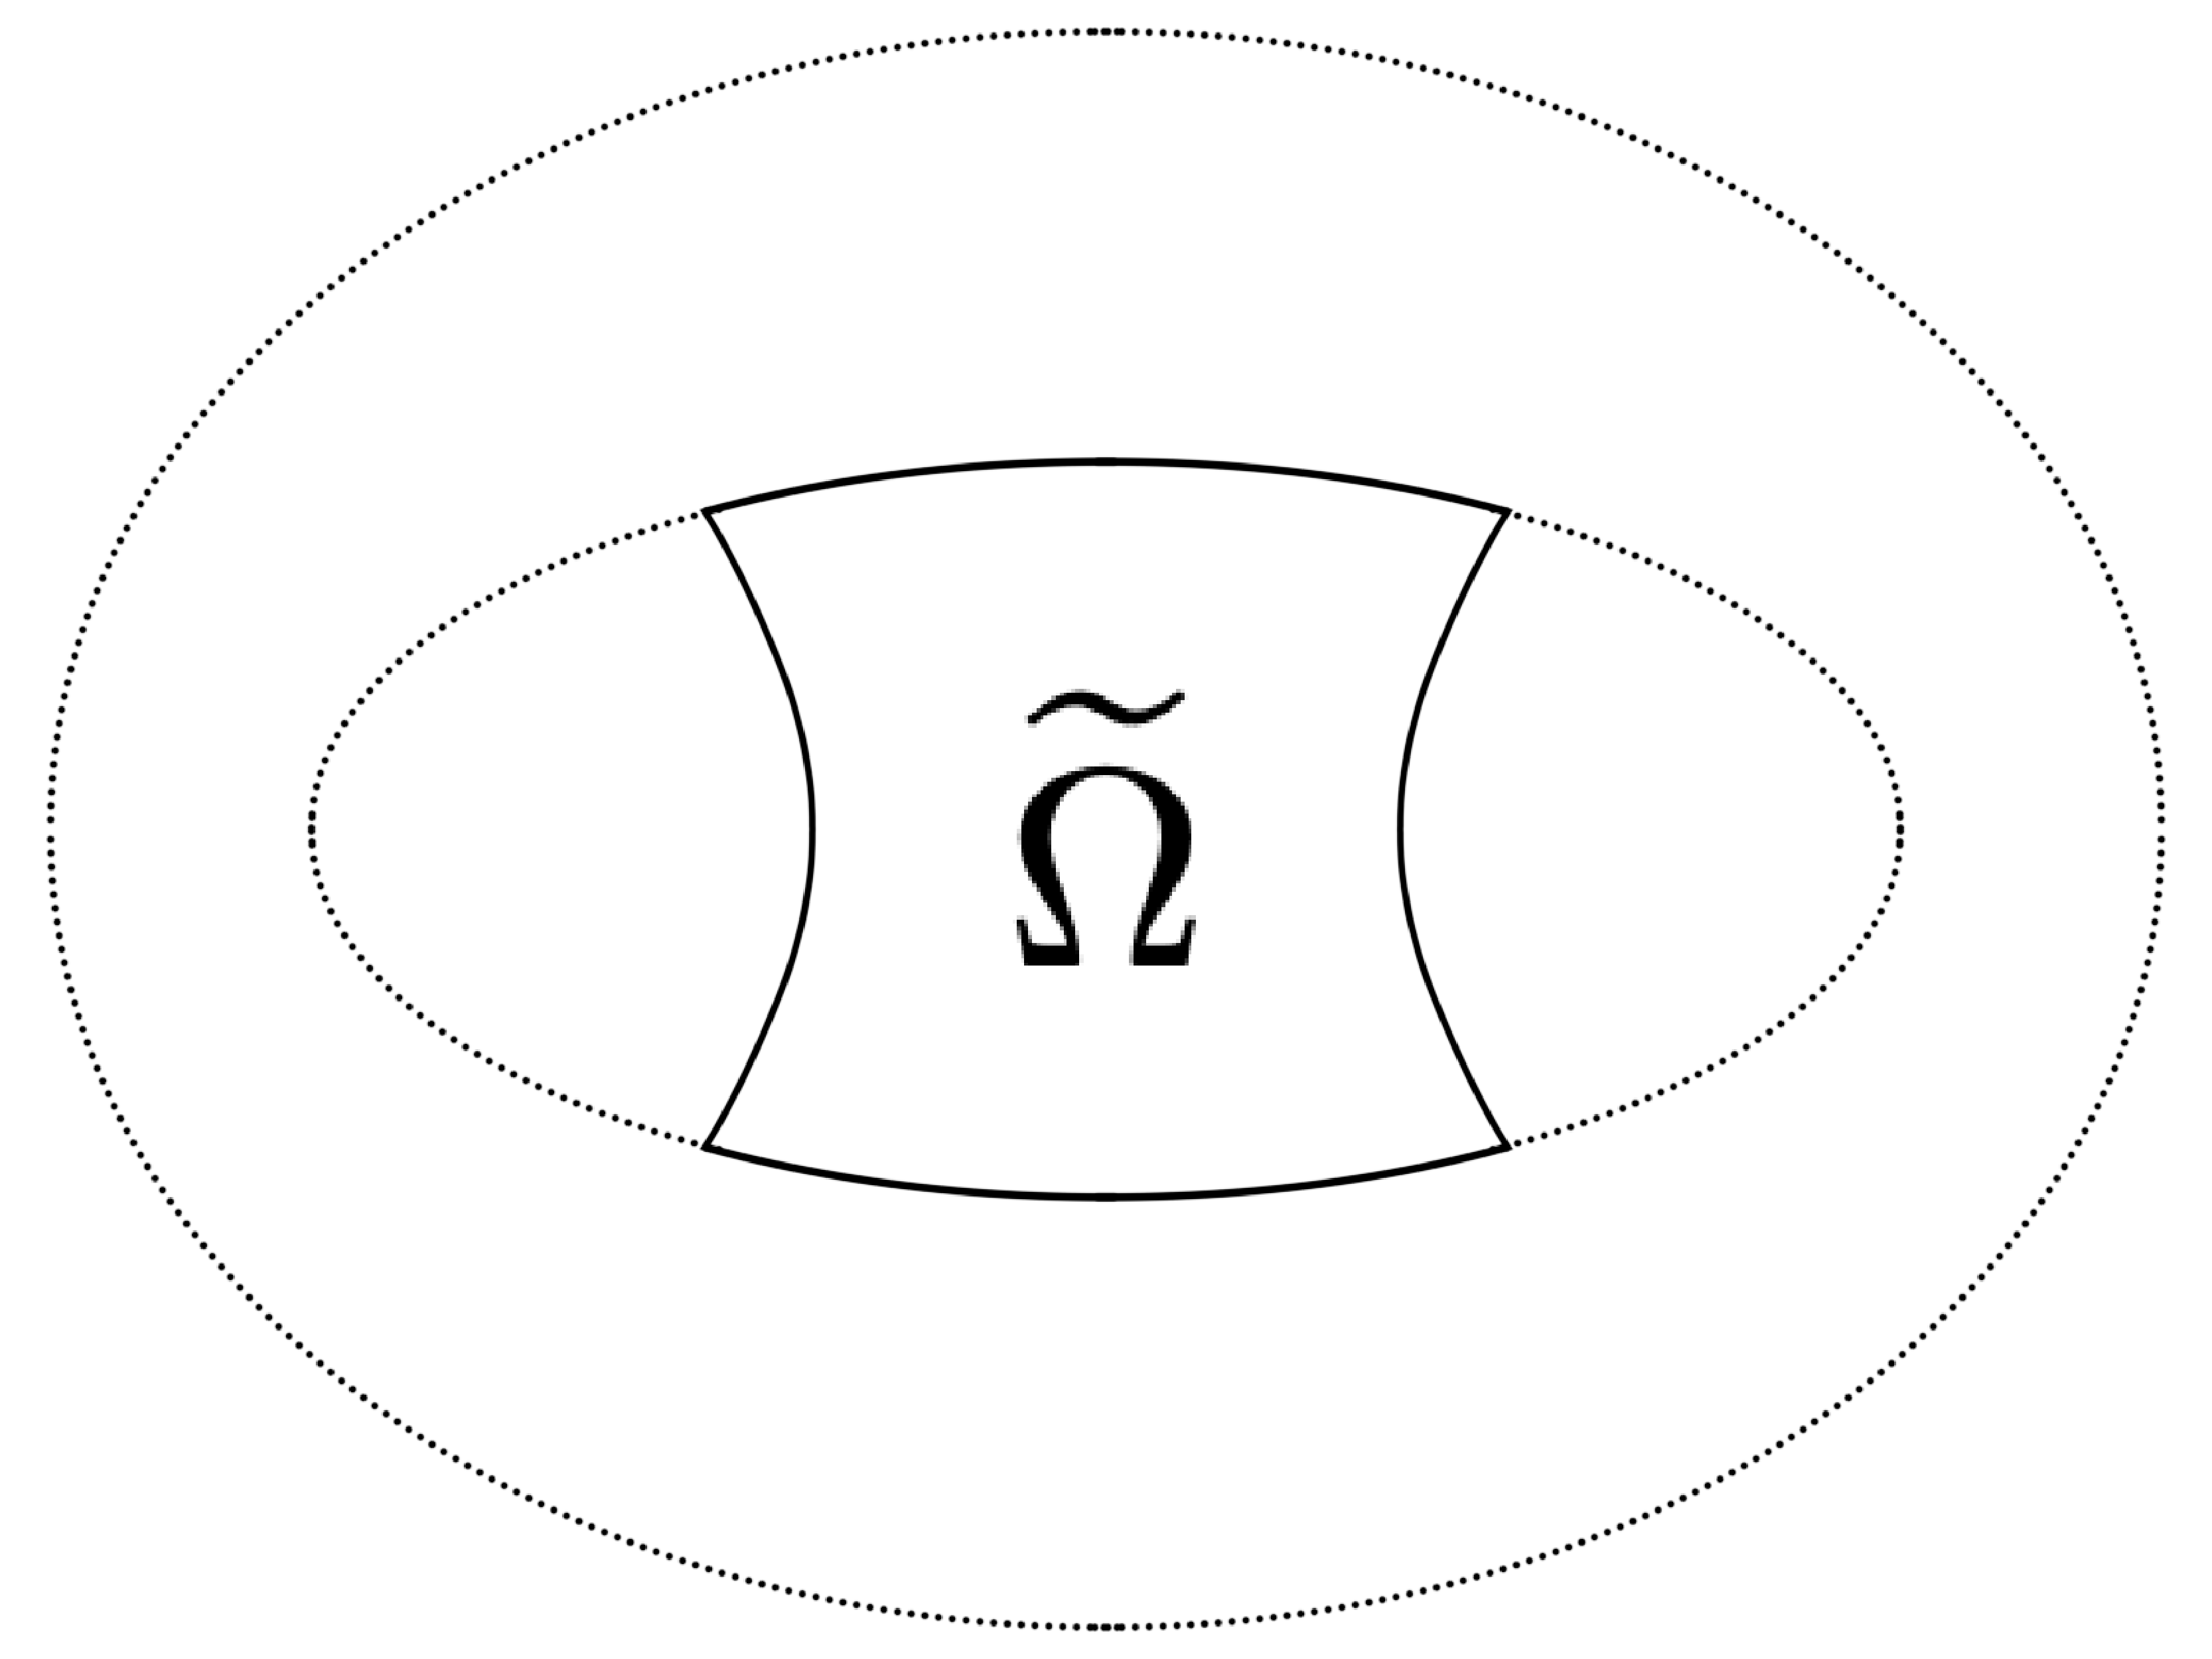
\includegraphics[width=0.8\linewidth]{images/ch4/section2/hyp_domain_example.pdf}
    \caption{Результирующая область $\widetilde{\Omega}$ для случая $D_3^2$.}
    \label{fig:pt9:_hyp_domain_example}
\endminipage\hfill
\minipage{0.45\textwidth}
\centering
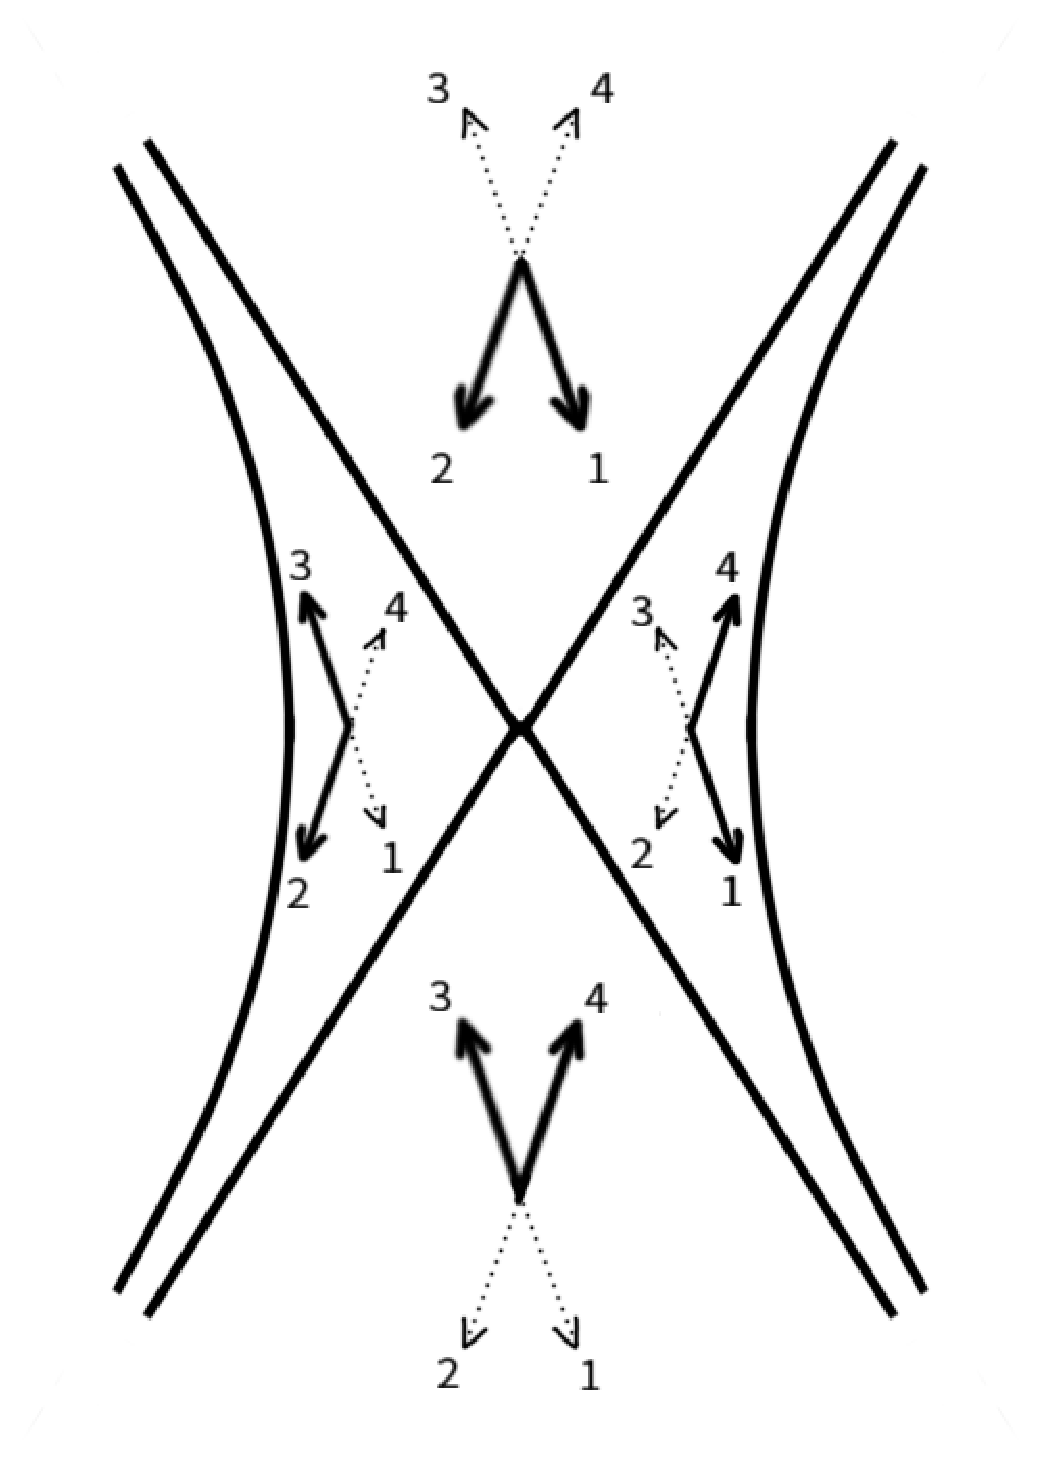
\includegraphics[width=0.65\linewidth]{images/ch4/section2/hyp_vectors_numbering.pdf}
    \caption{Направления векторов скорости $v_i$}
    \label{fig:pt9:_hyp_vectors_numbering}
\endminipage\hfill
\end{figure}

Граничные эллиптические дуги области $\widetilde{\Omega}_1$ склеиваются с одноименными эллиптическими дугами области $\widetilde{\Omega}_4$, аналогично для областей $\widetilde{\Omega}_2$, $\widetilde{\Omega}_3$.
Эти склейки дают нам две трубки.
Обе граничные гиперболы области $\widetilde{\Omega}_1$ отождествляются с соответствующими граничными гиперболами области $\widetilde{\Omega}_2$, аналогично для областей $\widetilde{\Omega}_3$ и $\widetilde{\Omega}_4$. Результатом склейки является один тор.

\medskip
\textbf{Случай $D_4^1$.} В этом случае проекция точки $(x, y, v_x, v_y)$, лежащей на поверхности $\Xi=\const$ при проекции $\pi$ заметает несвязную область, которая получается пересечением эллиптического кольца, ограниченного эллипсами $Q_{\lambda_1}$ и $Q_{0}$, и областью, содержащейся между ветвями гиперболы с параметром $\alpha_{out}$  (см. рис. \ref{fig:pt9:_d41_page}). 

Ясно, что определенная таким образом $\widetilde{\Omega}$ имеет две компоненты связности. Прообраз $\widetilde{\Omega}$ --- четыре листа $\widetilde{\Omega}_j, j=1, \ldots, 4$, где нумерация листов определена в соответствии с рис. \ref{fig:pt9:_hyp_vectors_numbering}. Каждый лист $\widetilde{\Omega}_j$ является  дизъюнктным объединением связных  листов $\widetilde{\Omega}_j^u \sqcup \widetilde{\Omega}_j^d$ (см. рис. \ref{fig:pt9:_d41_page}). 
%Упростим каждый лист склейки в соответствии с утверждением \ref{st:equivalent_borders} и получим рис. \ref{fig:pt9:_d41_page_simple}. 
Рассуждения, аналогичные рассуждениям предыдущего пункта, показывают, что для $i=1,\ldots, 4$ области $\widetilde{\Omega}_i^u$ склеиваются в один тор, а области $\widetilde{\Omega}_i^d$ --- в другой тор.

% повторяют склейки области $\widetilde{\Omega}$ в задаче $D_3^2$ и приводят к одному тору, аналогично результатом склейки четырех прямоугольников $\widetilde{\Omega}_i^d$ также является один тор.

\begin{figure}[!htb]
\centering
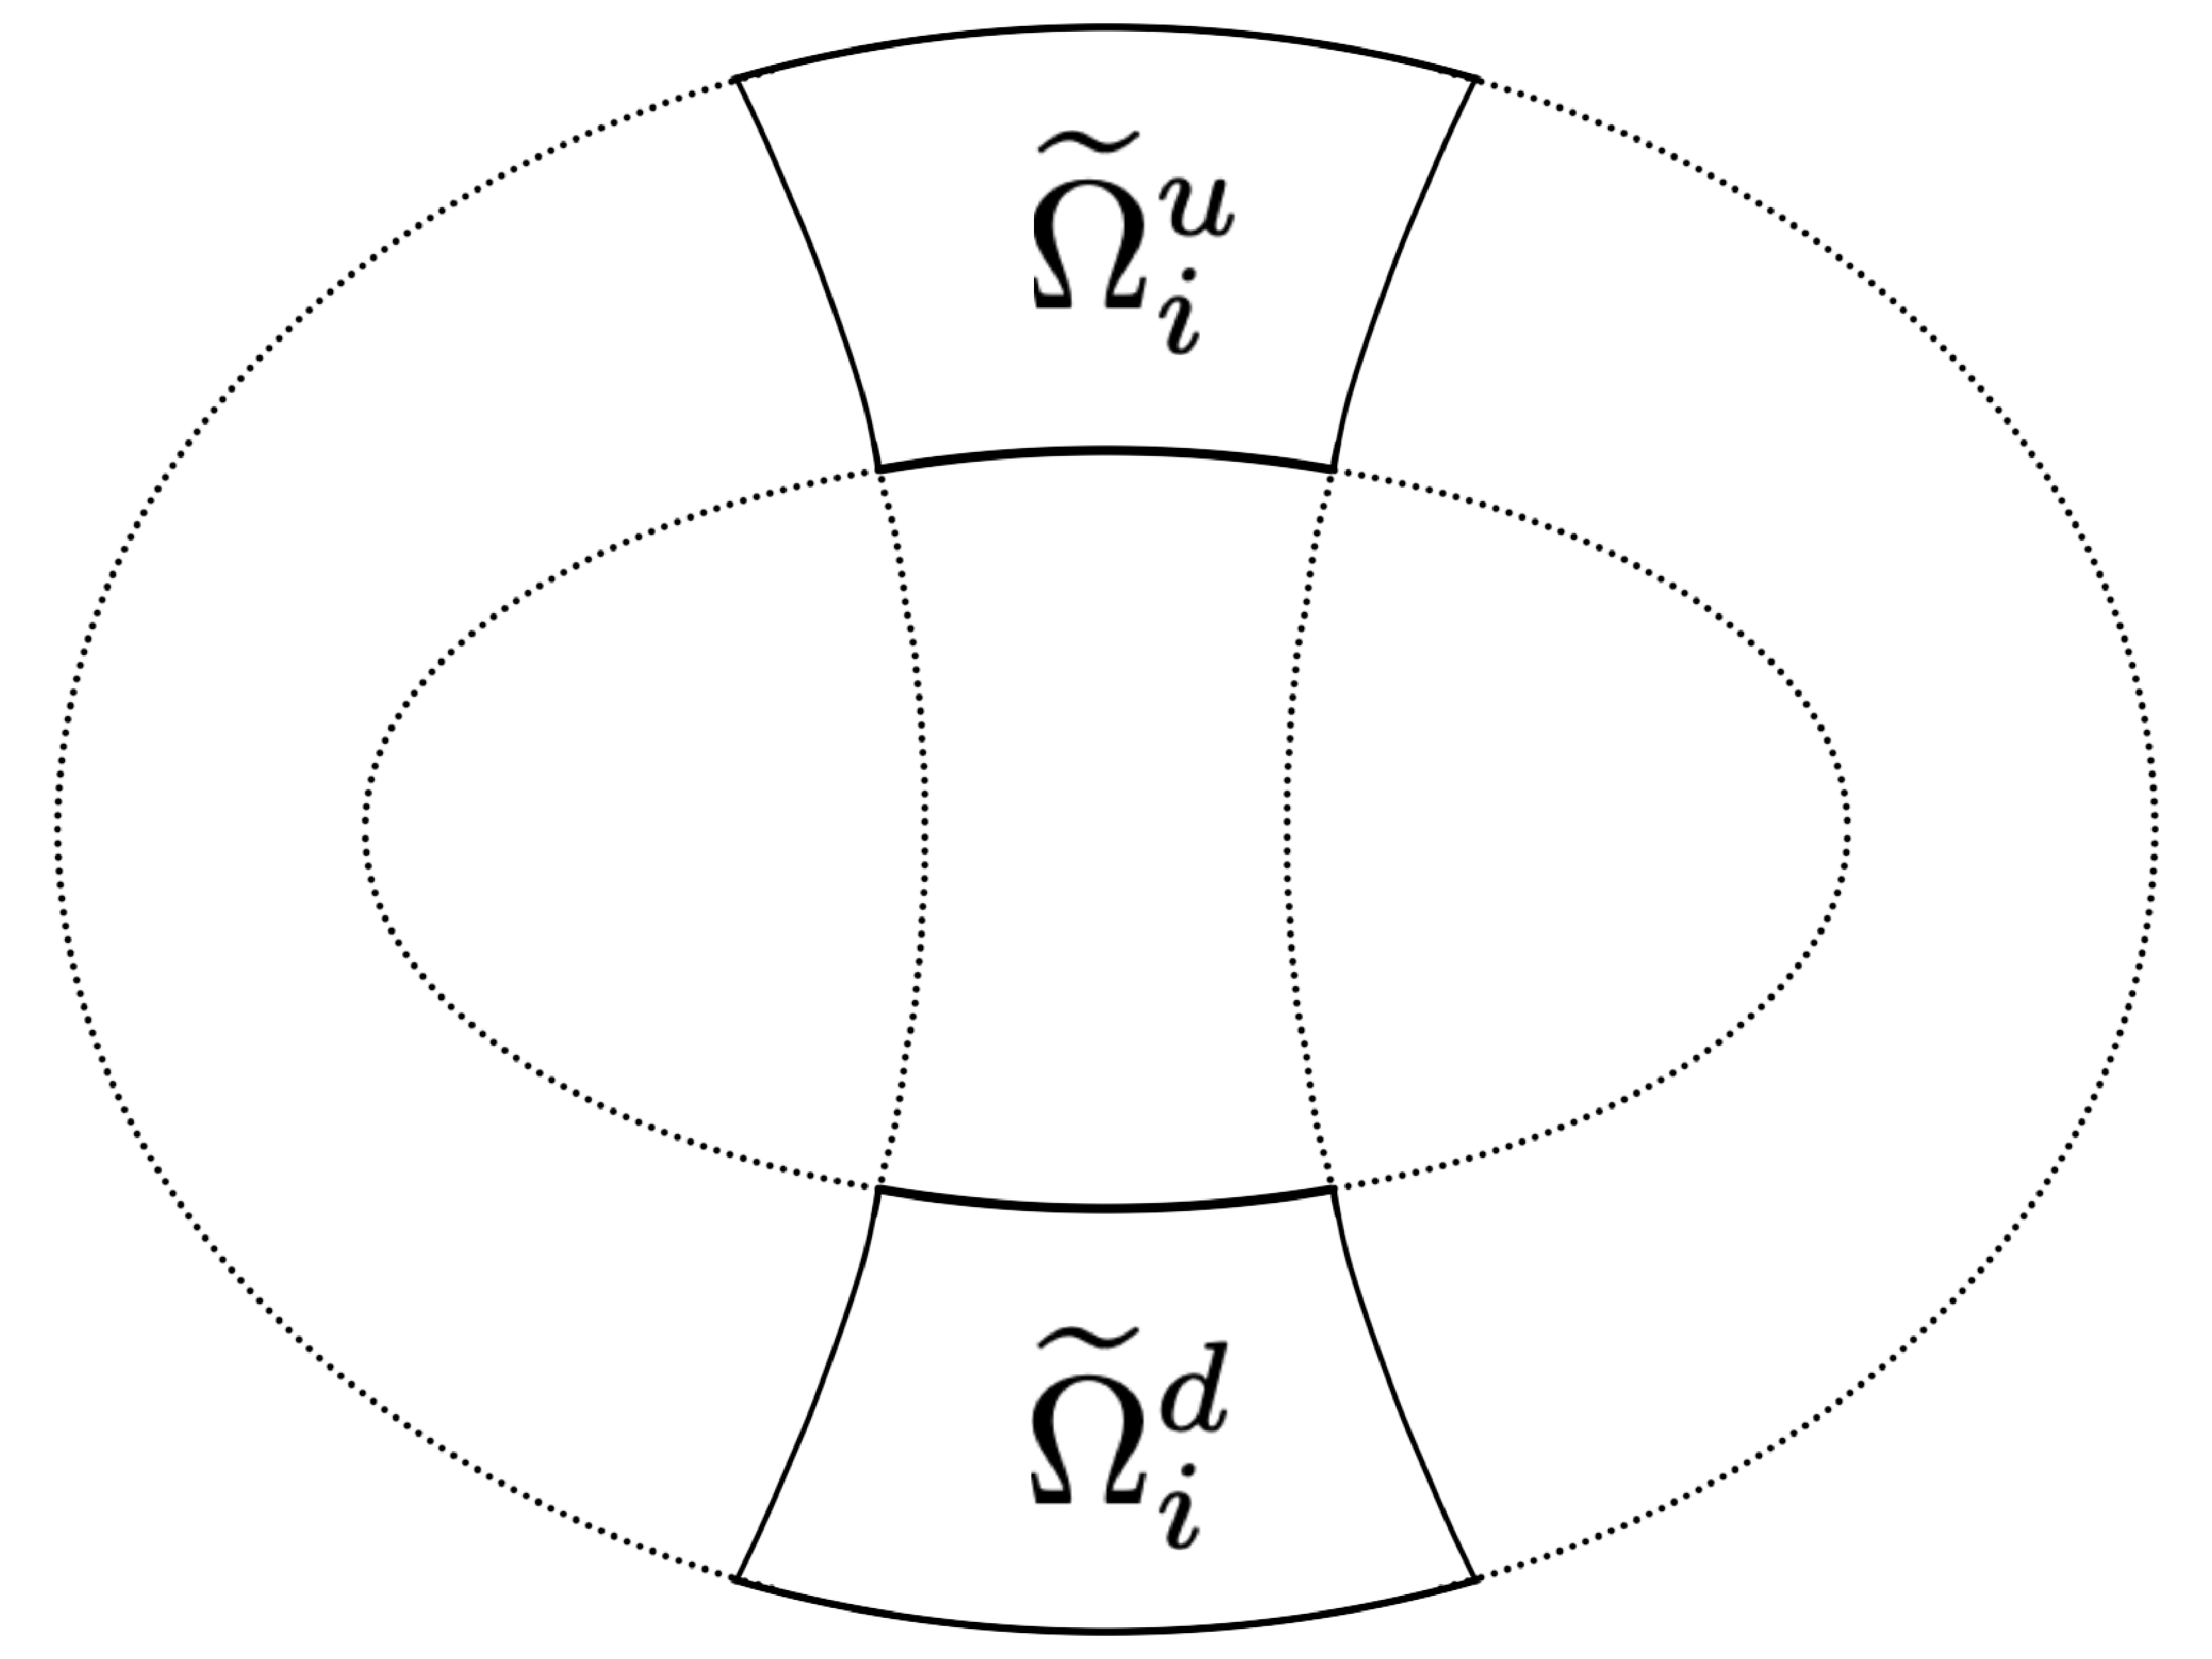
\includegraphics[width=0.35\linewidth]{images/ch4/section2/d41_page.pdf}
    \caption{Лист склейки  $\widetilde{\Omega}_i$  для случая $D_4^1$ состоит из двух областей.}
    \label{fig:pt9:_d41_page}
\end{figure}

\medskip
\textbf{Случай $D_1^2, D_1^3$. } 
Оба случая разбираются по одной схеме. 

Звенья и продолжения звеньев траектории, лежащие в $\Omega_{out}$, касаются гиперболы с параметром $\alpha_{out}$. Лежащие в $\Omega_{in}$ звенья и их продолжения касаются гиперболы с параметром $\alpha_{in}$.

Определим область $\widetilde{\Omega}_{in}$ как часть внутреннего эллипса $\Omega_{in}$, находящуюся между ветвей гиперболы $Q_{\alpha_{in}}$. Положим $\widetilde{\Omega}_{out}$ --- пересечение эллиптического кольца $\Omega_{out}$ с областью, лежащей между ветвями гиперболы с параметром $\alpha_{out}$; $\widetilde{\Omega}_{out}$ имеет две компоненты связности.

Проекция бильярдной траектории в эллиптической области заметает $\widetilde{\Omega} = \widetilde{\Omega}_{in} \cup \widetilde{\Omega}_{out}$ (см. рис.     \ref{fig:pt9:_img17}). Относительно проекции $\pi$ прообраз $\widetilde{\Omega}$ состоит из 4 листов $\widetilde{\Omega}_j, \ j=1, \ldots, 4$. 
Нумерацию листов снова сделаем в соответствии с рис. \ref{fig:pt9:_hyp_vectors_numbering}.

\begin{figure}[!htb]
\minipage{0.43\textwidth}
\centering
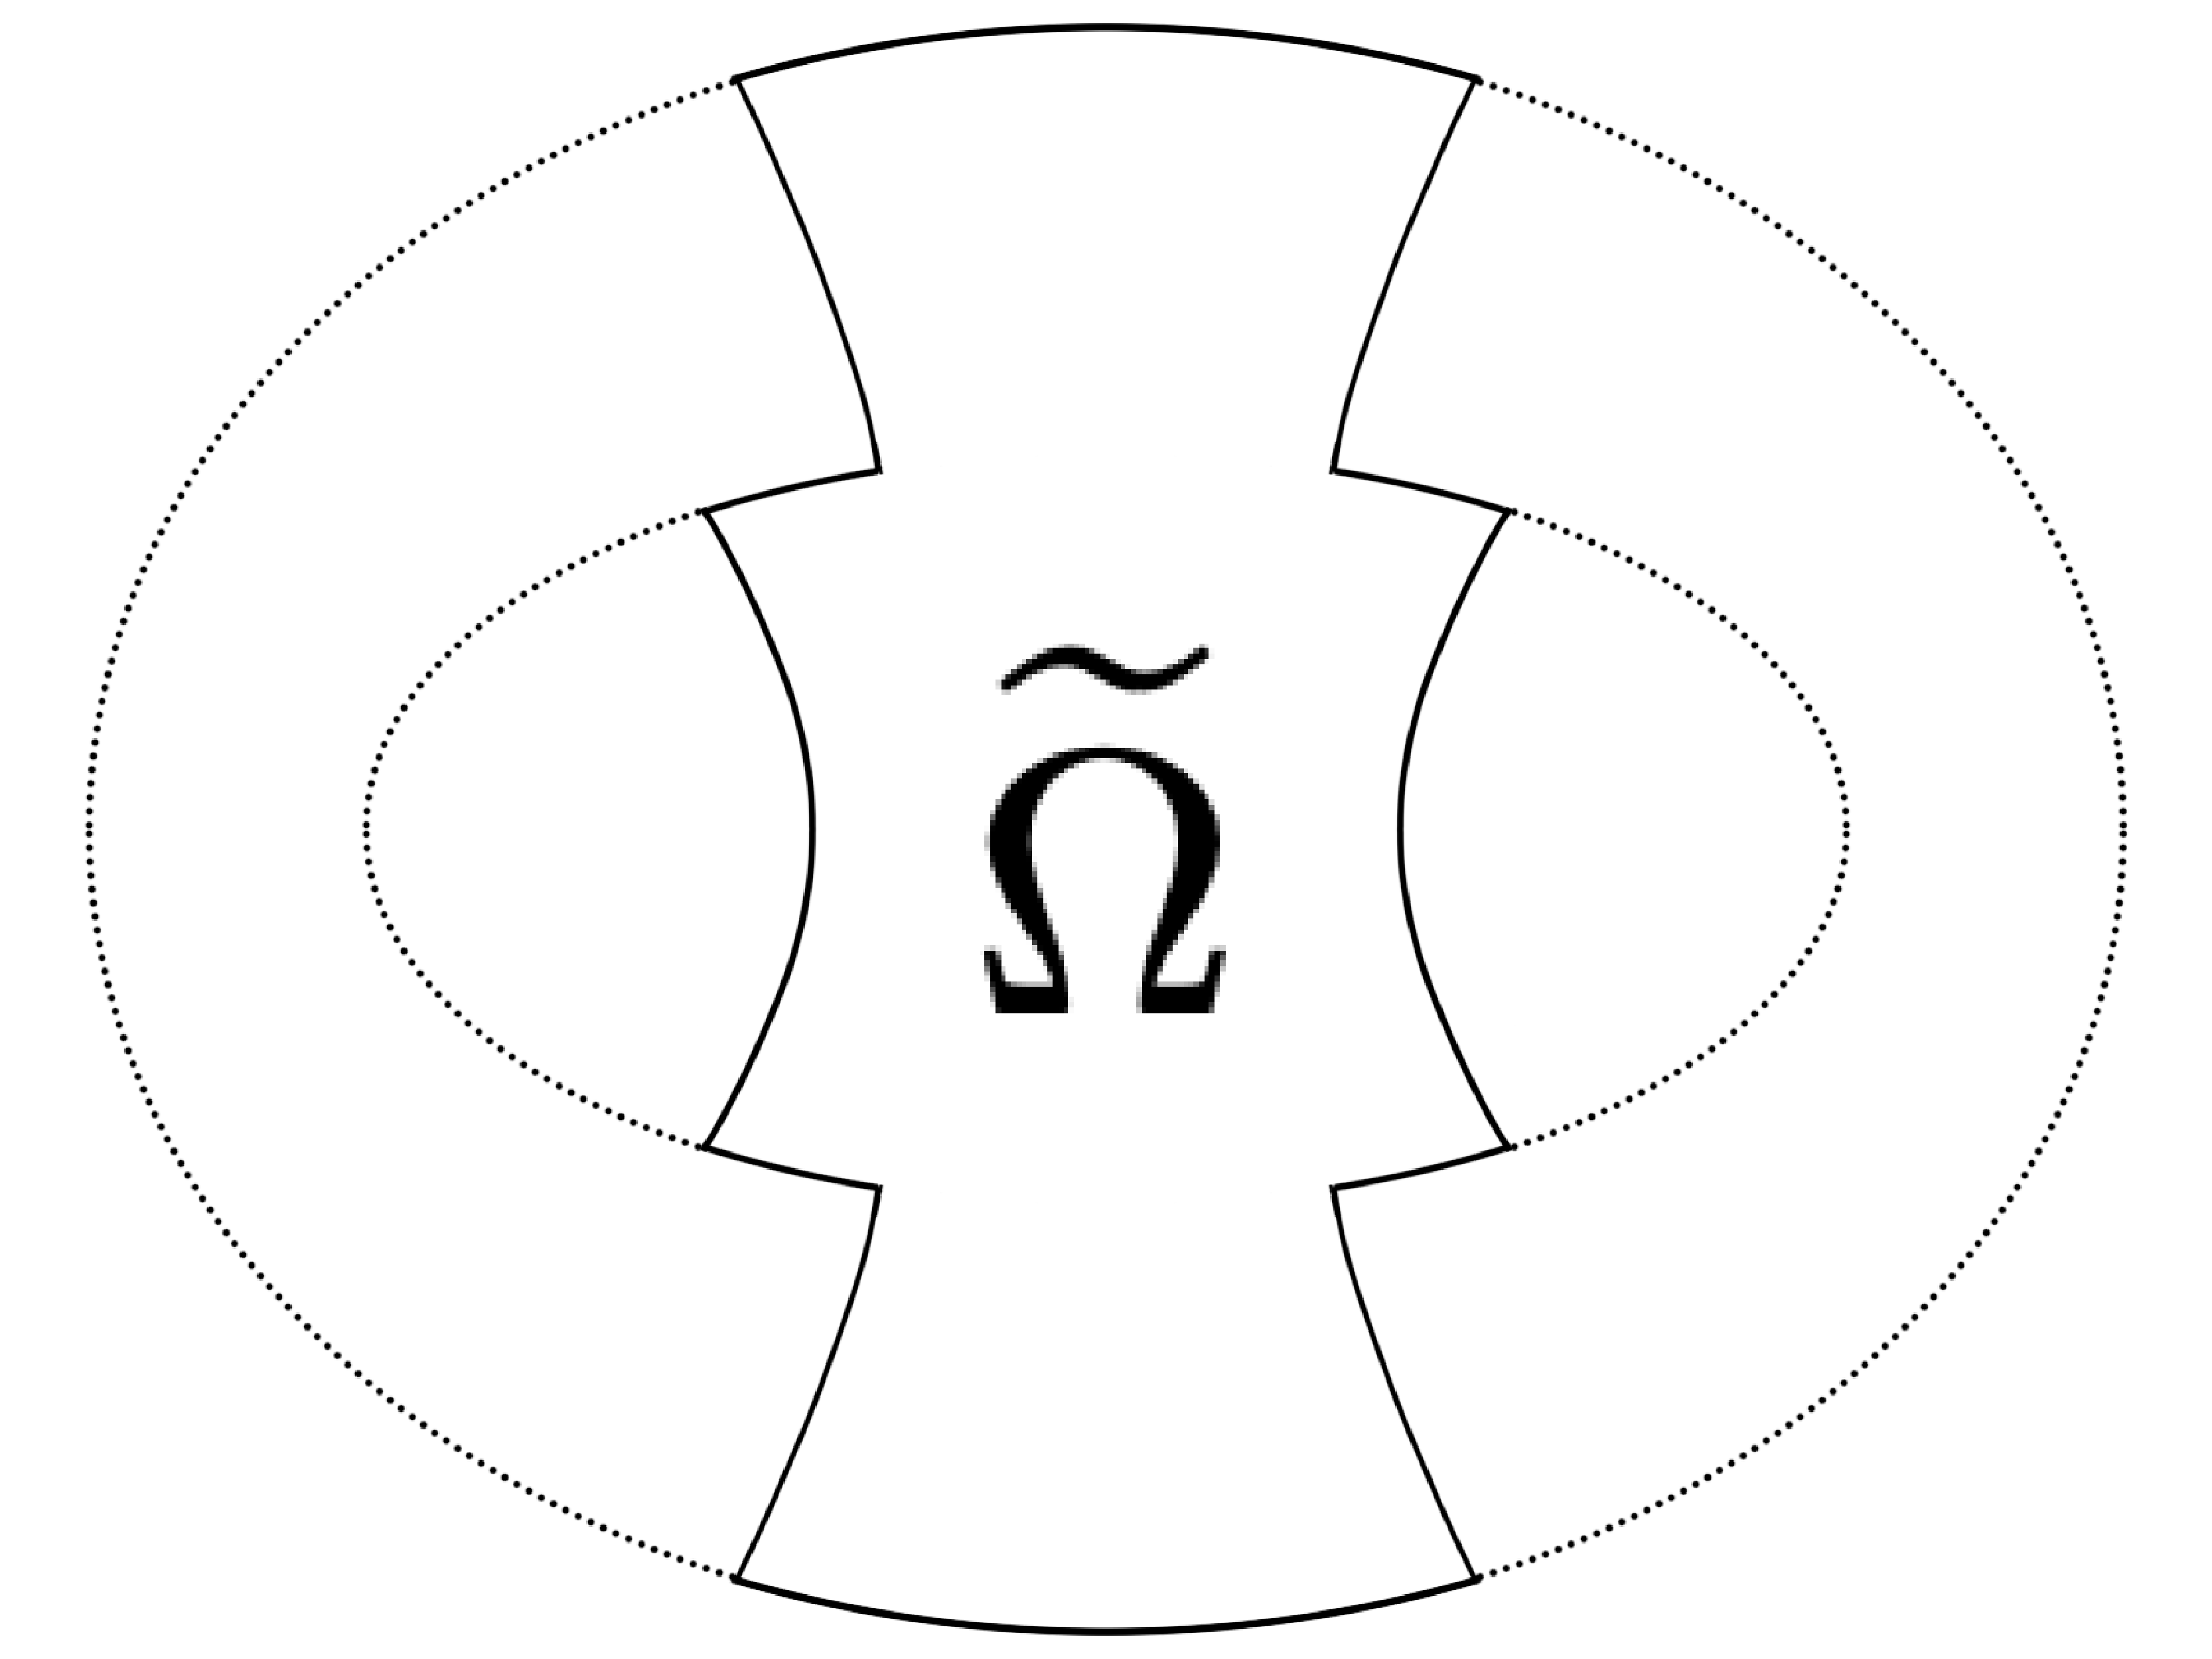
\includegraphics[width=0.7\linewidth]{images/ch4/section2/img17.pdf}
    \caption{Область $\widetilde{\Omega}$ для случая $D_1^2$.}
    \label{fig:pt9:_img17}
\endminipage\hfill
\minipage{0.42\textwidth}
\centering
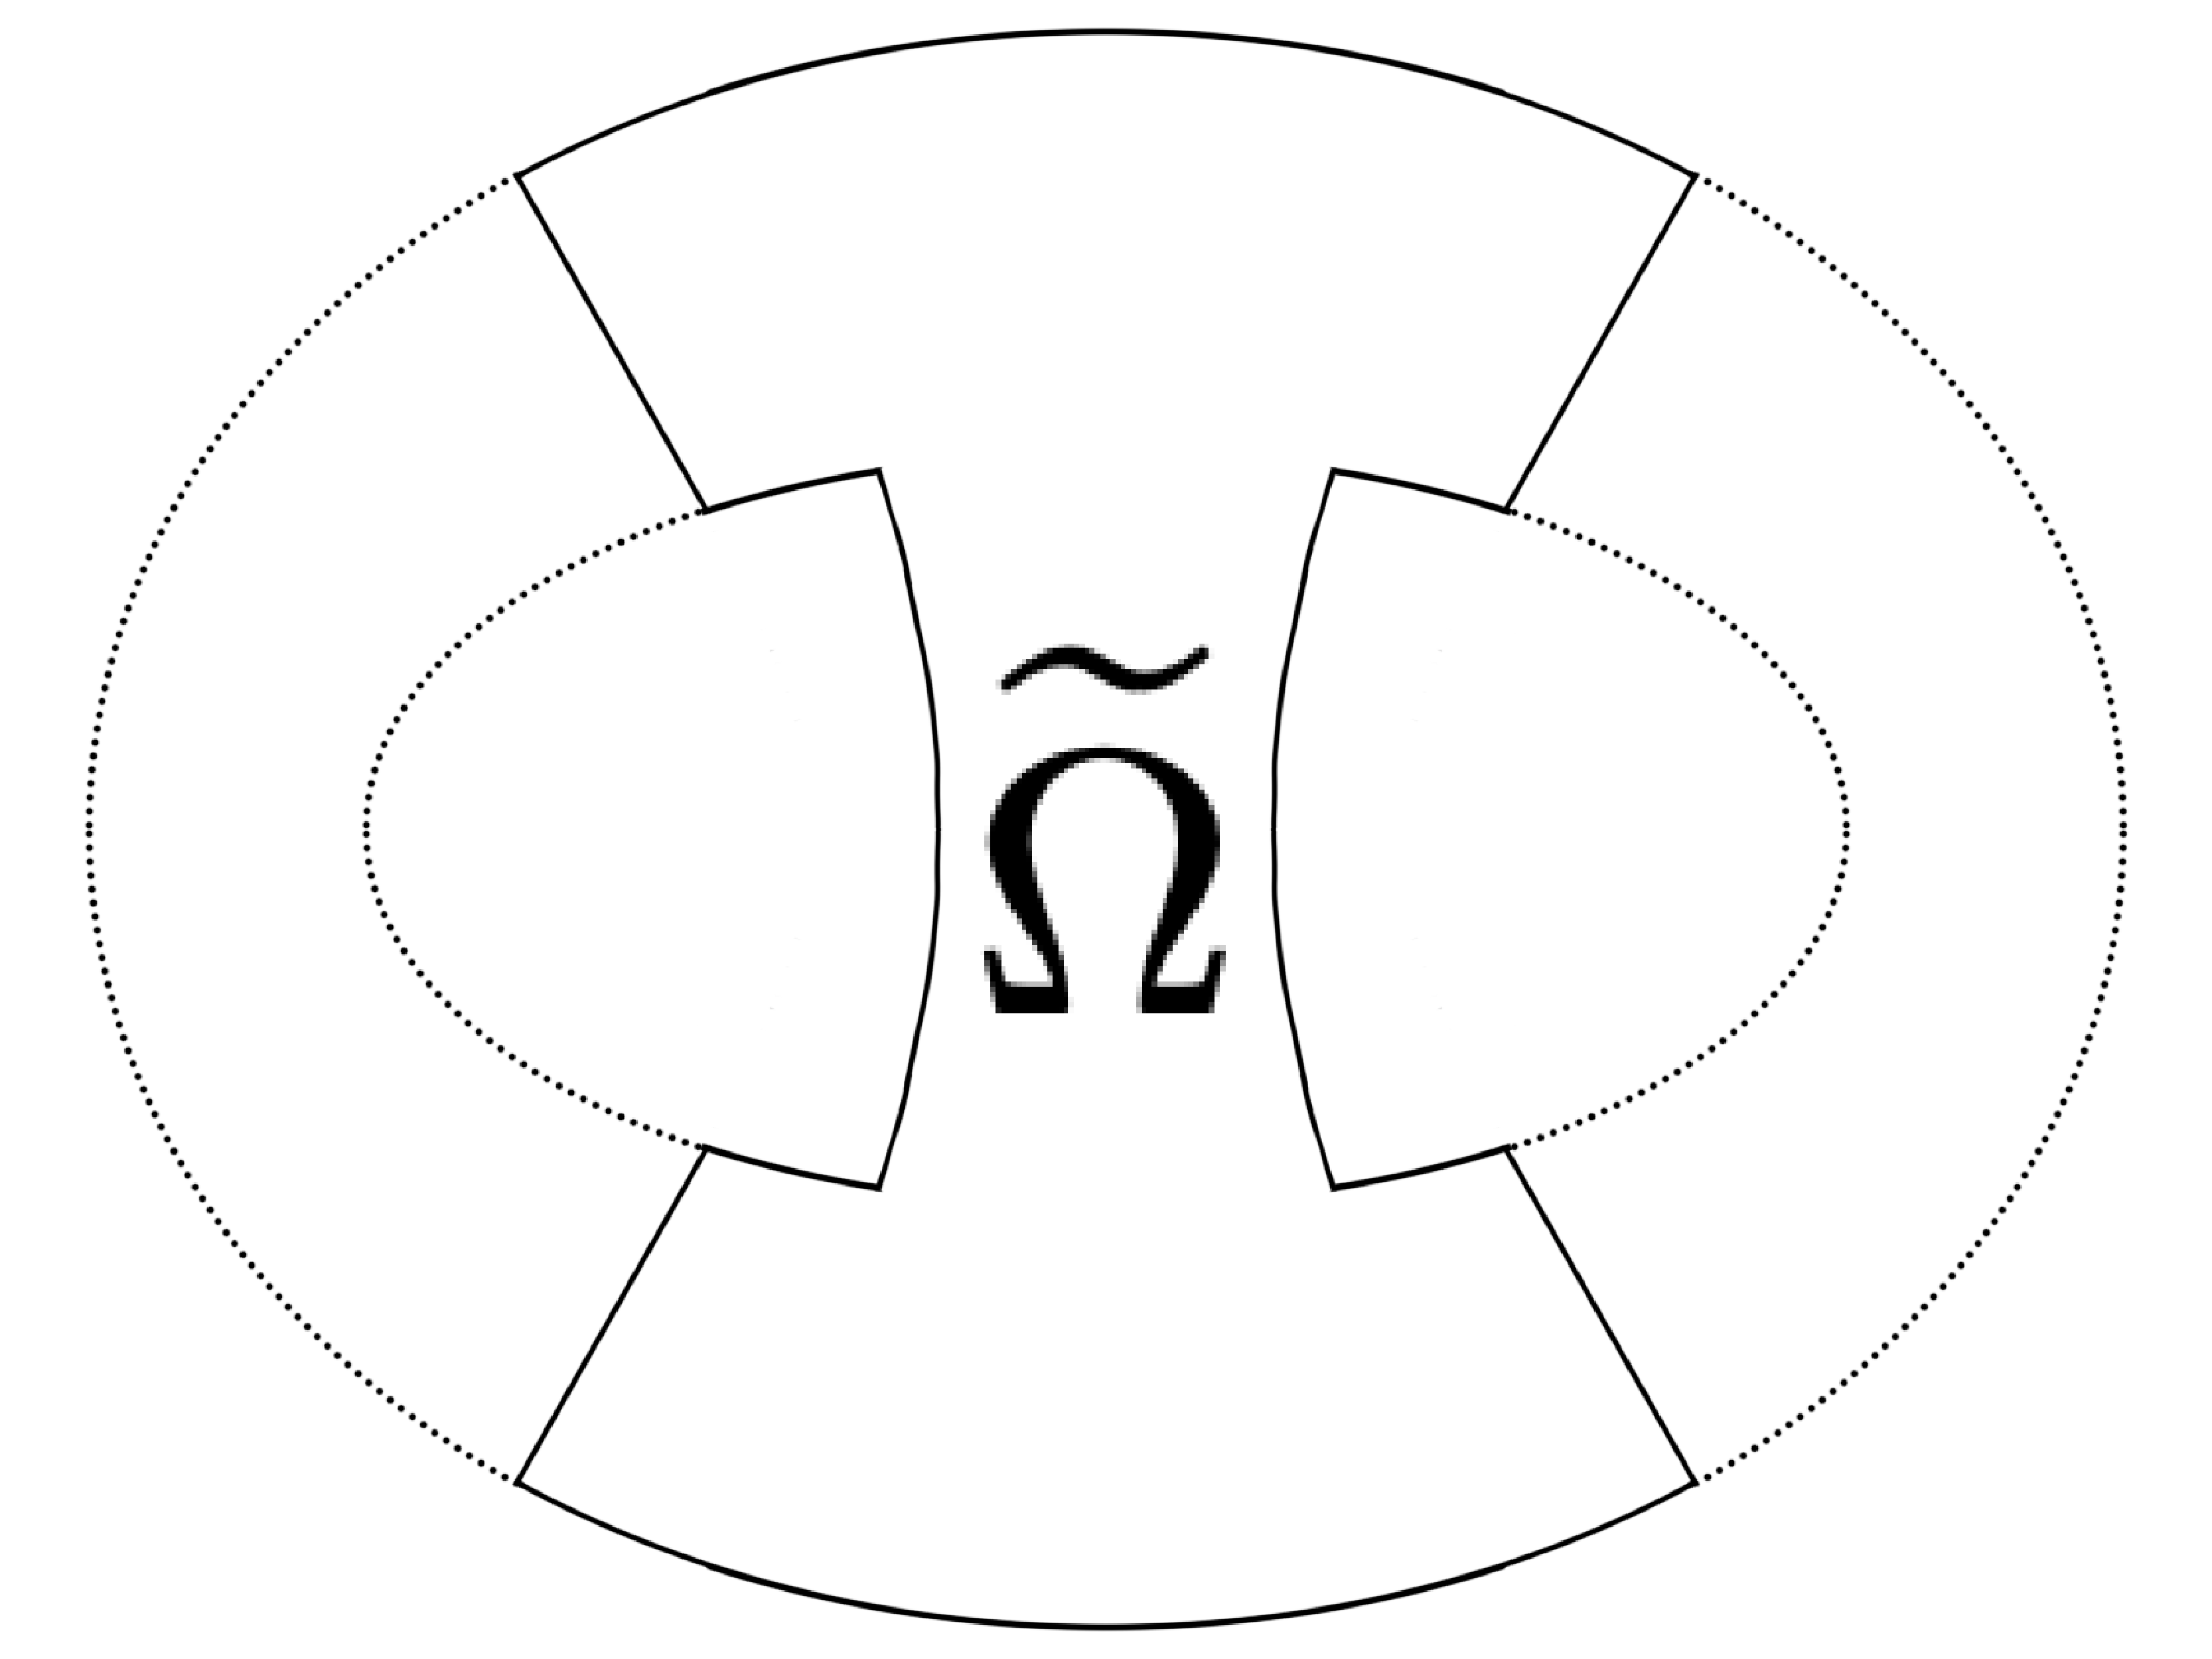
\includegraphics[width=0.7\linewidth]{images/ch4/section2/img18.pdf}
    \caption{Область $\widetilde{\Omega}$ для случая $D_1^3$.}
    \label{fig:pt9:_img18}
\endminipage\hfill
\end{figure}




Поверхность $\Xi=\const$ склеена из $\widetilde{\Omega}_1, \ldots, \widetilde{\Omega}_4$.
Шесть граничных эллиптических дуг области $\widetilde{\Omega}_1$ склеиваются с соответствующими граничными эллиптическими дугами области $\widetilde{\Omega}_4$. Аналогично для областей $\widetilde{\Omega}_2$ и $\widetilde{\Omega}_3$.
Результатом этих склеек являются две сферы с шестью дырками каждая.
Каждая дырка ограничивается двумя дугами, проектирующимися в одну граничную гиперболическую дугу области $\widetilde{\Omega}$.

Остается отождествить края этих дырок. Для этого заметим, что граничные гиперболические дуги области $\widetilde{\Omega}_1$ отождествляются с соответствующими граничными гиперболами области $\widetilde{\Omega}_2$, аналогичное справедливо для областей $\widetilde{\Omega}_3$ и $\widetilde{\Omega}_4$. Результатом этих склеек является сфера с пятью ручками. 

\medskip
\textbf{Случай $D_1^1$.}
Звенья траектории бильярда, лежащие в области $\Omega_{out}$, лежат на касательных к гиперболе с параметром $\alpha_{out}$, в то время как сегменты траектории, находящиеся в области $\Omega_{in}$, касаются эллипса с параметром $\alpha_{in}$. 

Определим область $\widetilde{\Omega}_{in} = \Omega_{in} \setminus \Omega_{\alpha_{in}}$ (эллиптическое кольцо), а область $\widetilde{\Omega}_{out}$ определим как пересечение эллиптического кольца $\Omega_{out}$ с областью, лежащей между ветвями гиперболы с параметром $\alpha_{out}$; $\widetilde{\Omega}_{out}$ имеет две компоненты связности
(см.  предыдущий случай): $\widetilde{\Omega}_{out} = \widetilde{\Omega}_{out}^u \sqcup \widetilde{\Omega}_{out}^d$.

Поверхность $\Xi = \const$ склеена из областей 
$\widetilde{\Omega}_{in, j}$, $\widetilde{\Omega}_{out, j}^u$,  $\widetilde{\Omega}_{out, j}^d, \ j=1, \ldots, 4$. Здесь листы  $\widetilde{\Omega}_{out, j}^u, \widetilde{\Omega}_{out, j}^d$ занумерованы в соответствии с рис. \ref{fig:pt9:_hyp_vectors_numbering}. Листы $\widetilde{\Omega}_{in, j}$ занумерованы в соответствии с правилом  \eqref{eq:ell_numeration}.

Области $\widetilde{\Omega}_{out, j}^u$ и $\widetilde{\Omega}_{in, j}$ отождествляются по общей граничной дуге, которую проекция $\pi$ отображает в дугу 
$\partial \widetilde{\Omega}_{out}^u \cap \partial \widetilde{\Omega}_{in}$.
В симметрично расположенную дугу эллипса в нижней полуплоскости проекция $\pi$ отображает граничные дуги, на которых отождествляются следующие пары областей: 
$\widetilde{\Omega}_{out, 1}^d$ с $\widetilde{\Omega}_{in, 3}$,
$\widetilde{\Omega}_{out, 3}^d$ с $\widetilde{\Omega}_{in, 1}$,
$\widetilde{\Omega}_{out, 2}^d$ с $\widetilde{\Omega}_{in, 4}$ и 
$\widetilde{\Omega}_{out, 4}^d$ с $\widetilde{\Omega}_{in, 2}$.

Таким образом, поверхность $\Xi = \const$ склеена из четырех листов:
$\widetilde{\Omega}_1 = \widetilde{\Omega}_{out, 1}^u \cup \widetilde{\Omega}_{in, 1} \cup \widetilde{\Omega}_{out, 3}^d$, 
$\widetilde{\Omega}_2 = \widetilde{\Omega}_{out, 2}^u \cup \widetilde{\Omega}_{in, 2} \cup \widetilde{\Omega}_{out, 4}^d$, 
$\widetilde{\Omega}_3 = \widetilde{\Omega}_{out, 3}^u \cup \widetilde{\Omega}_{in, 3} \cup \widetilde{\Omega}_{out, 1}^d$ и 
 $\widetilde{\Omega}_4 = \widetilde{\Omega}_{out, 4}^u \cup \widetilde{\Omega}_{in, 4} \cup \widetilde{\Omega}_{out, 2}^d$ (лист $\widetilde{\Omega}_1$ показан на рис. \ref{fig:pt9:_hyp_page}).
 \begin{figure}[!htb]
 \centering
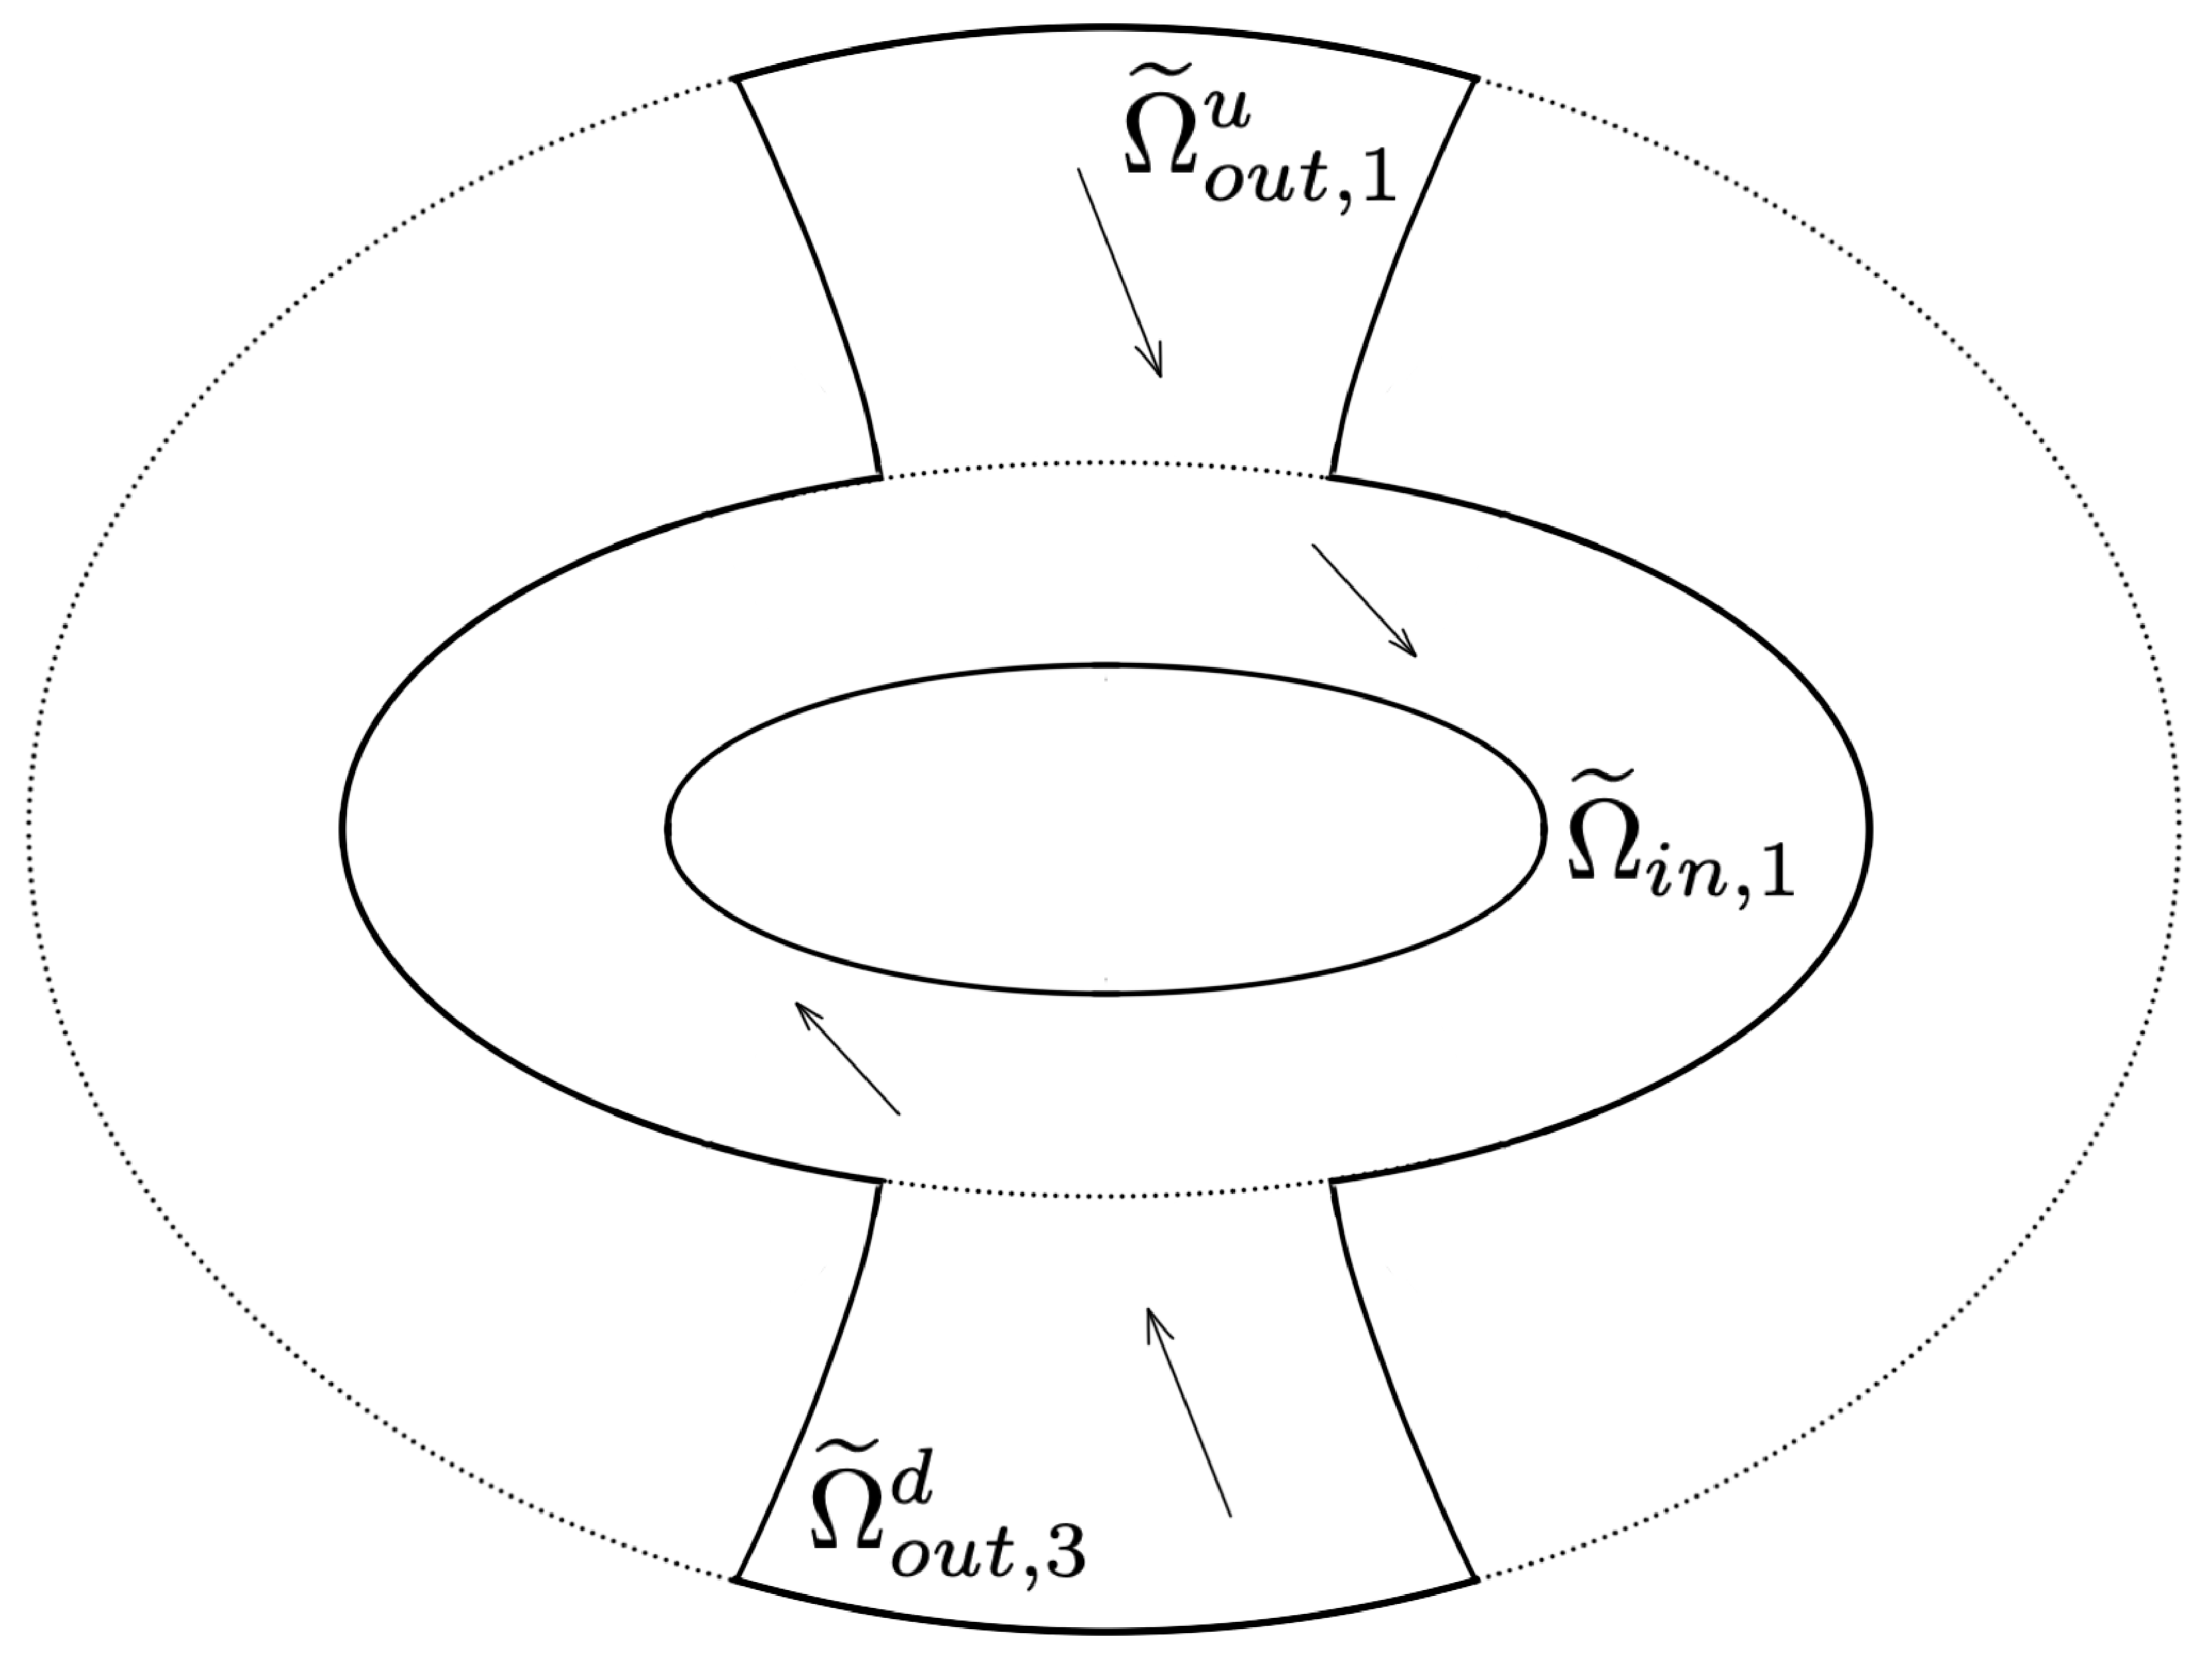
\includegraphics[width=0.4\linewidth]{images/ch4/section2/problems_vectors_2.pdf}
    \caption{Лист склейки $\widetilde{\Omega}_1$.}
    \label{fig:pt9:_hyp_page}
\end{figure}

 
Граничные эллиптические дуги области $\widetilde{\Omega}_1$  склеиваются с соответствующими эллиптическими дугами  области $\widetilde{\Omega}_4$, аналогично для областей $\widetilde{\Omega}_2$ и $\widetilde{\Omega}_3$. Результатом этих склеек являются два тора с четыремя дырками каждый. 
Каждая дырка ограничивается двумя дугами, проектирующимися в одну граничную гиперболическую дугу области $\widetilde{\Omega} = \widetilde{\Omega}_{in} \cup \widetilde{\Omega}_{out}$.

Остается отождествить края этих дырок. Для этого заметим, что граничные гиперболические дуги области $\widetilde{\Omega}_1$ отождествляются с одноименными граничными гиперболами области $\widetilde{\Omega}_2$, аналогичное справедливо для областей $\widetilde{\Omega}_3$ и $\widetilde{\Omega}_4$. Результатом этих склеек является сфера с пятью ручками. 

\textbf{Случай $D_1^6$}.
Продолжения звеньев бильярдной траектории, лежащие в $\Omega_{out}$, касаются эллипса с параметром $\alpha_{out}$, а сегменты траектории, находящиеся в $\Omega_{in}$, касаются гиперболы с параметром $\alpha_{in}$. 

Определим область $\widetilde{\Omega}_{in}$ как пересечение эллипса $\Omega_{in}$ и области, лежащей между двумя ветвями гиперболы с параметром $\alpha_{in}$.
Поверхность  $\Xi = \const$ проектируется на объединение $\widetilde{\Omega}_{in} \cup \Omega_{out}$. 
Каждой внутренней точке этой области соответствуют четыре точки-прообраза на поверхности $\Xi = \const$.
Тем самым, поверхность $\Xi = \const$ склеена из областей $\widetilde{\Omega}_{in, j}, \Omega_{out, j}, \ j=1,\ldots,4$.
Здесь области $\Omega_{out, j}$ нумеруются в соответствии с правилом \eqref{eq:ell_numeration}, а области $\widetilde{\Omega}_{in, j}$ нумеруются согласно рис. \ref{fig:pt9:_hyp_vectors_numbering}.


В силу закона преломления $(\ast)$ области $\widetilde{\Omega}_{in, j}$ и $\Omega_{out, j}$ для каждого $j=1,\ldots, 4$ отождествляются по общему участку границы, который проекция $\pi$ отображает в дугу эллипса $Q_{\lambda_1}$, а именно, в дугу $\partial \widetilde{\Omega}_{in} \cap \partial \Omega_{out}$, находящуюся в верхней полуплоскости.
В симметричную ей дугу в нижней полуплоскости проектируются общие участки границы для областей $\widetilde{\Omega}_{in, 1}$ и $\Omega_{out, 3}$ в силу того же закона $(\ast)$. Аналогично отождествляются области $\widetilde{\Omega}_{in, 2}$ и $\Omega_{out, 4}$, $\widetilde{\Omega}_{in, 3}$ и $\Omega_{out, 1}$, а также $\widetilde{\Omega}_{in, 4}$ и $\Omega_{out, 2}$.

Определим листы $\widetilde{\Omega}_j$, $j=1, \ldots, 4$ (пример см. рис. \ref{fig:pt9:_ell_and_hyp_2}) следующим образом: 
$\widetilde{\Omega}_j = \widetilde{\Omega}_{in, j} \cup \Omega_{out, j}$, где объединение листов осуществляется по общей дуге, проецирующейся на верхнюю дугу эллипса $Q_{\lambda_1}$.

\begin{figure}[!htb]
\minipage{0.4\textwidth}
\centering
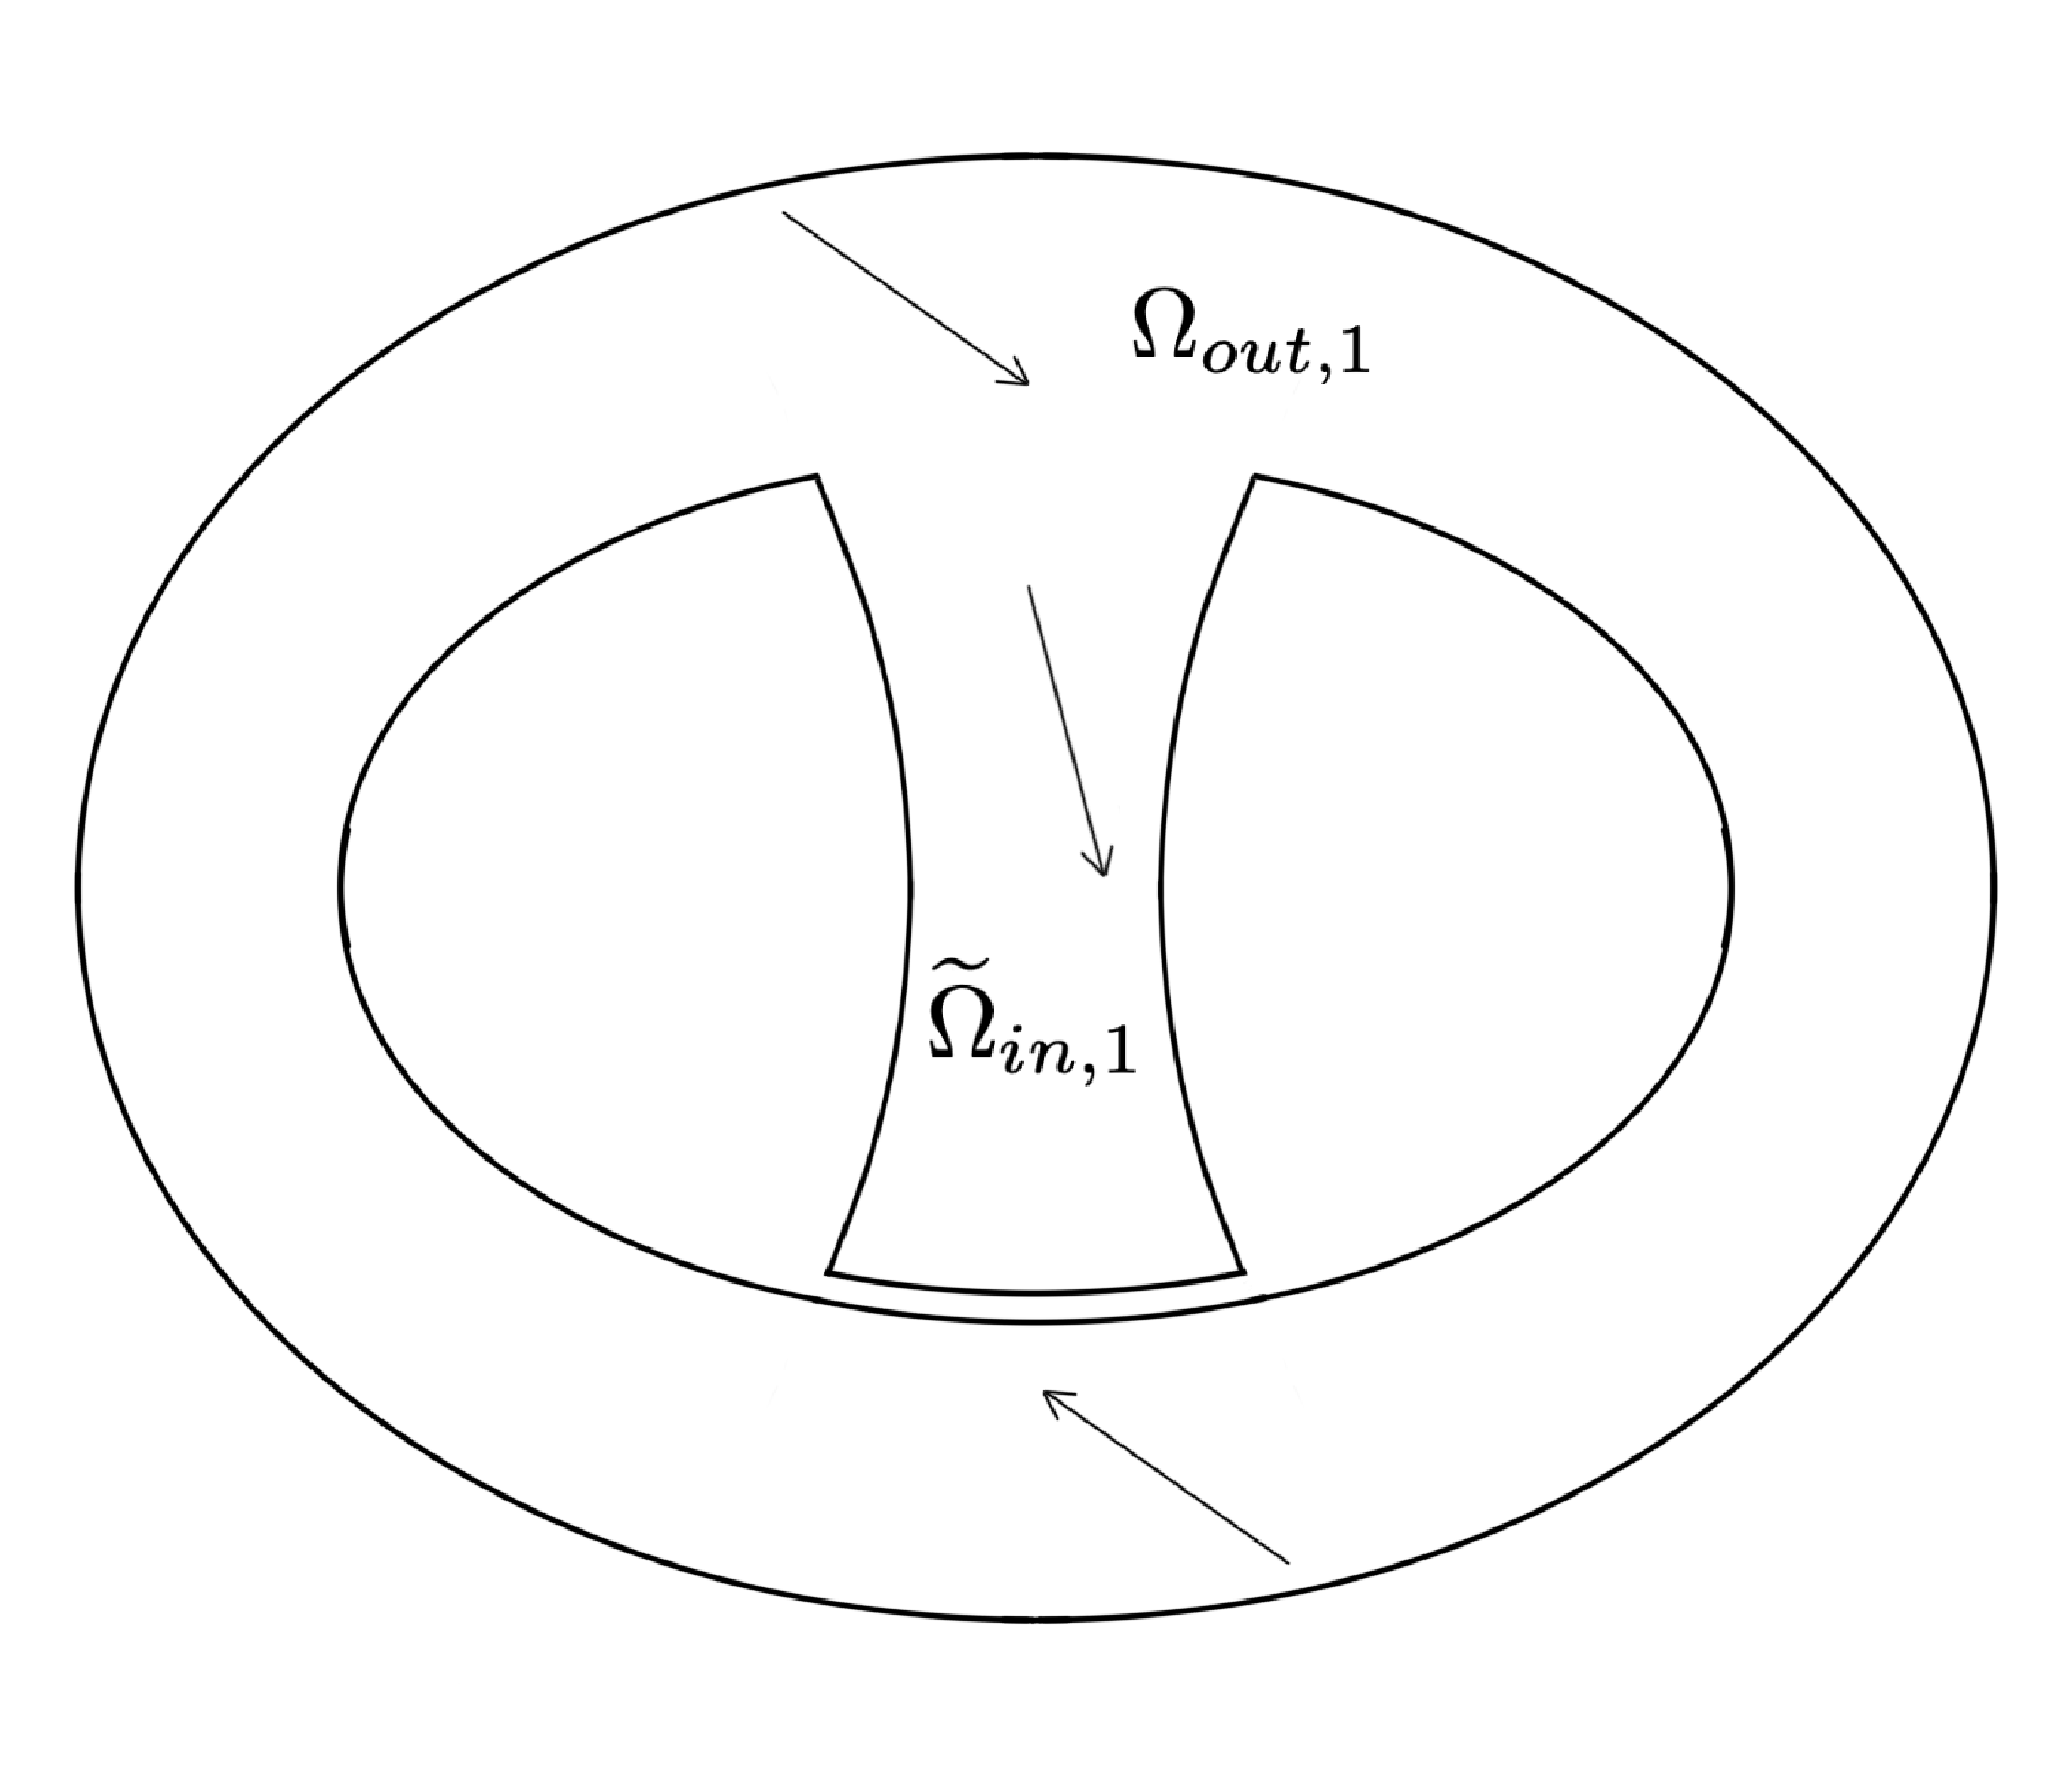
\includegraphics[width=5cm]{images/ch4/section2/ell_and_hyp2.pdf}
    \caption{Область $\widetilde{\Omega}_1$.}
    \label{fig:pt9:_ell_and_hyp_2}
\endminipage\hfill
\minipage{0.6\textwidth}
\centering
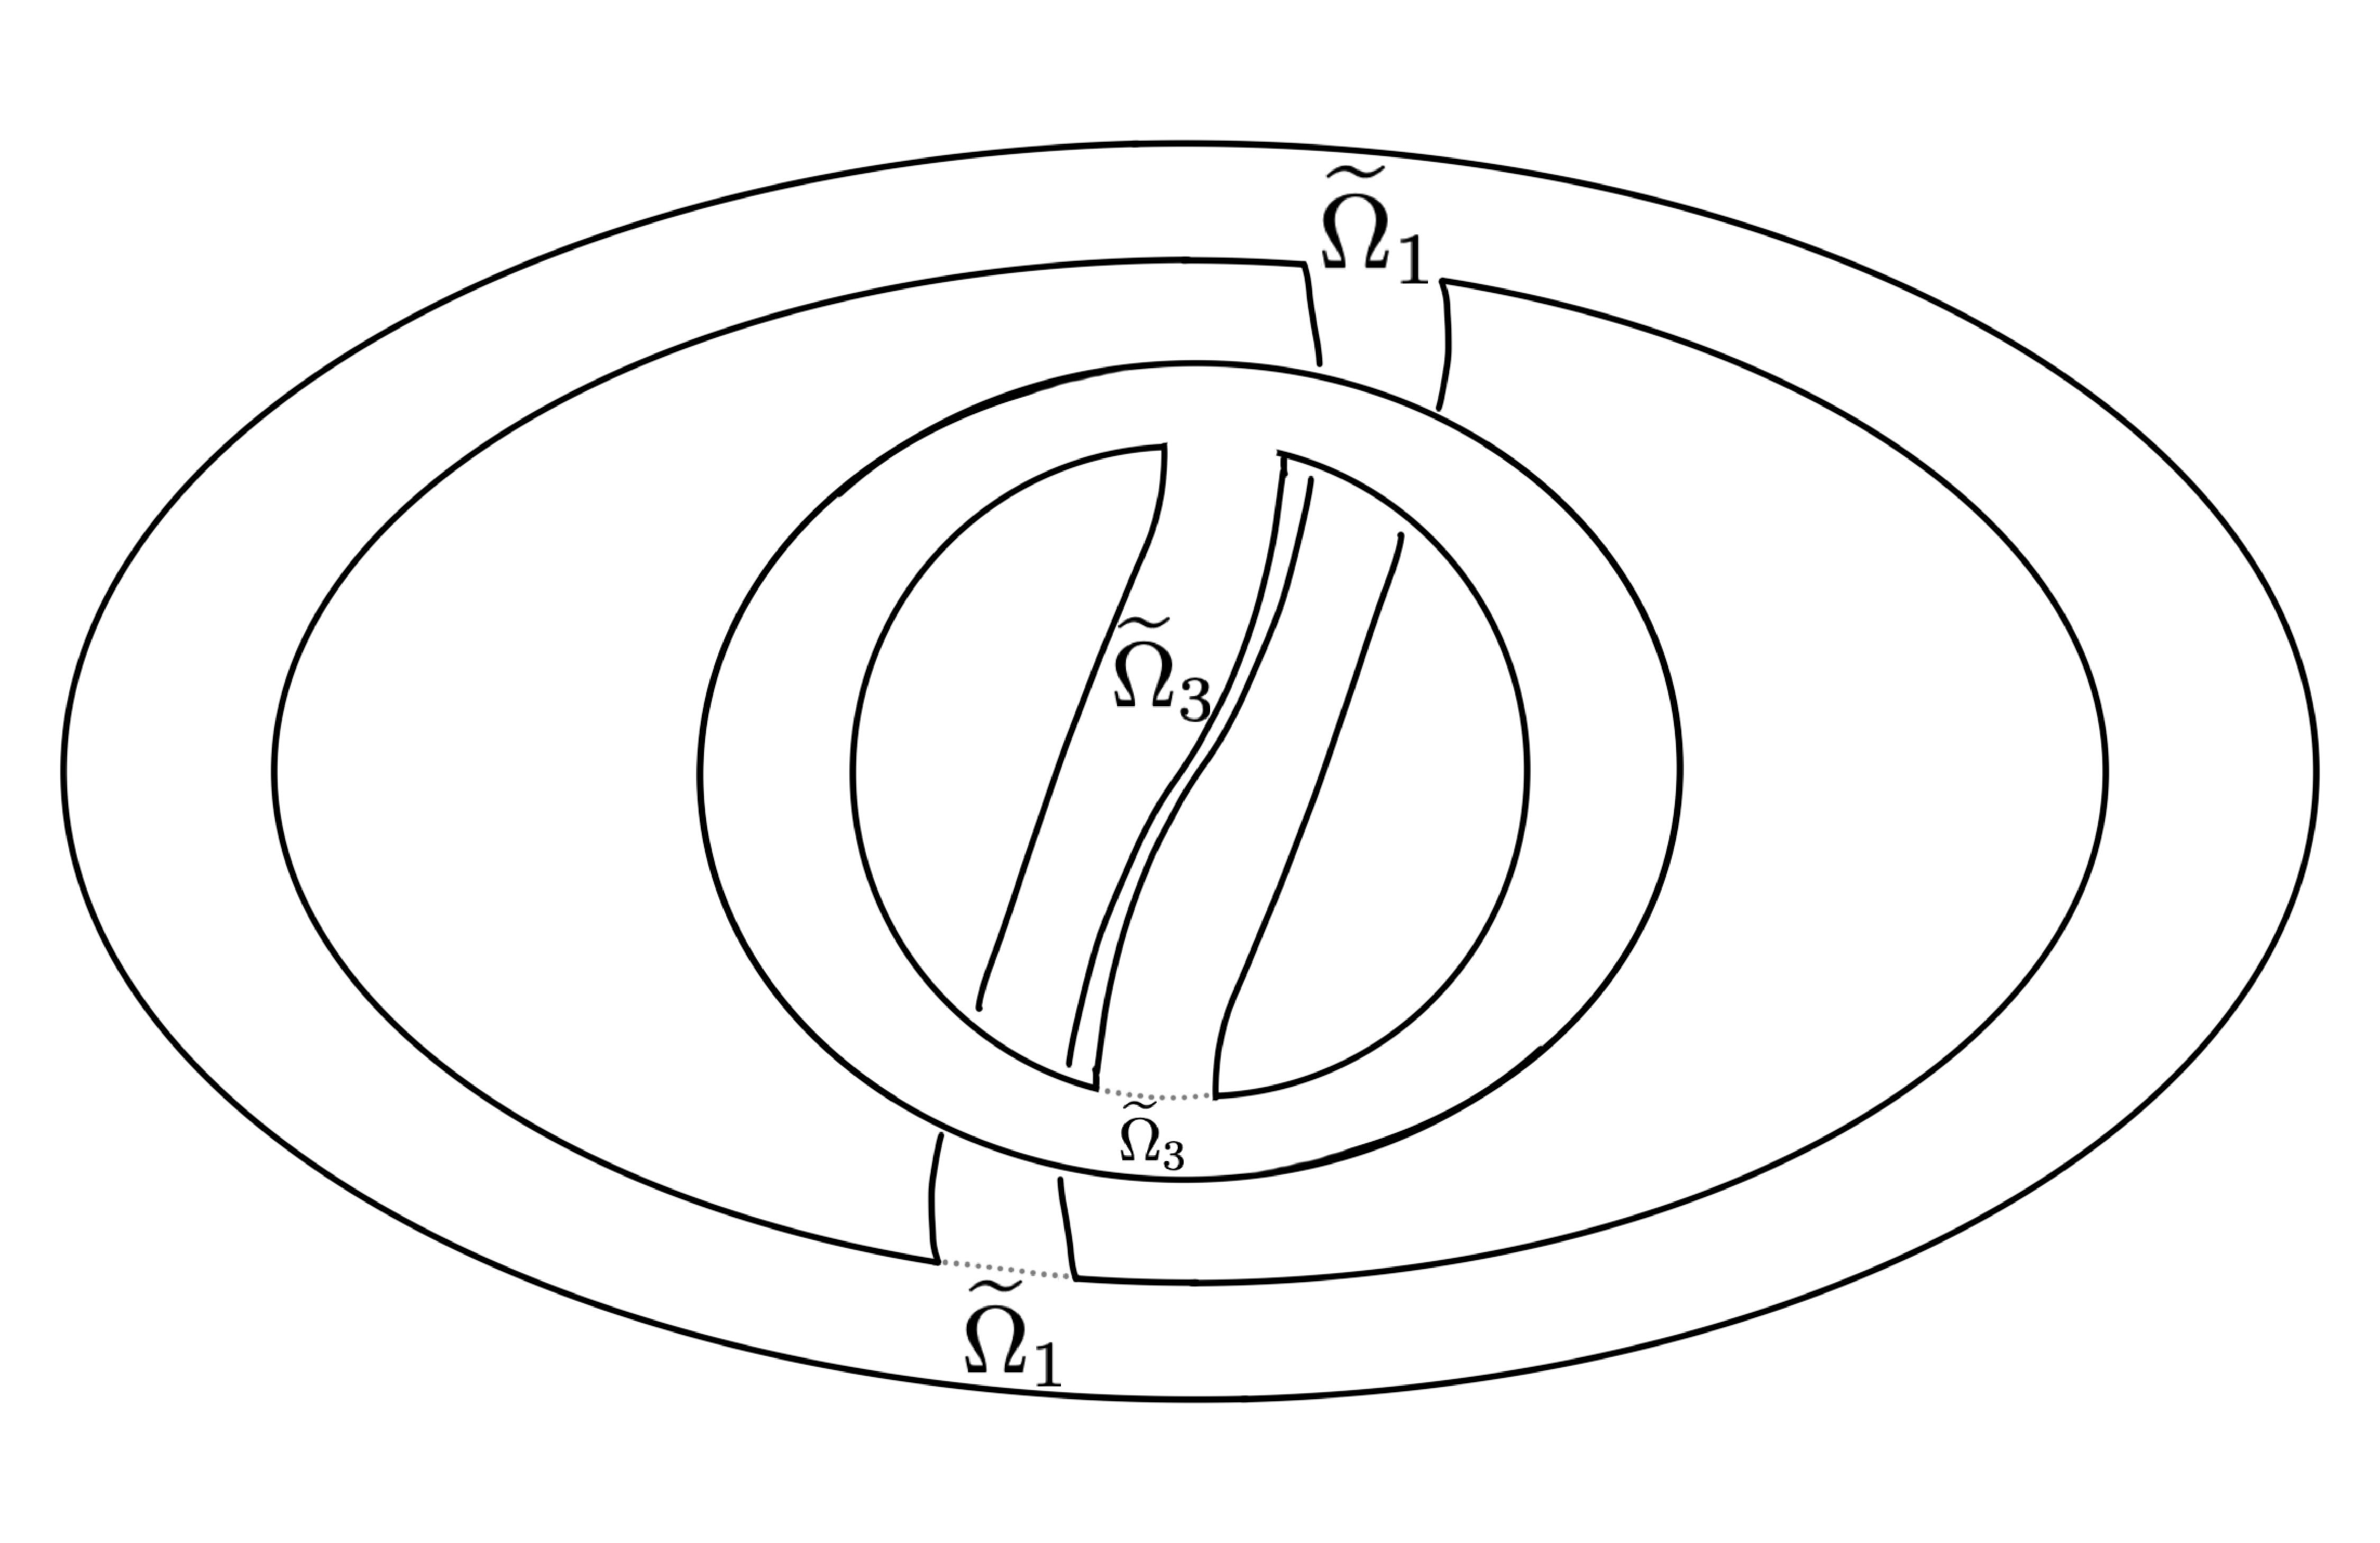
\includegraphics[width=7cm]{images/ch4/section2/ell_and_hyp2_permutations.pdf}
    \caption{Результат склейки $\widetilde{\Omega}_1$ и $\widetilde{\Omega}_3$ (одно эллиптическое кольцо уменьшено для наглядности).}
    \label{fig:pt9:_ell_and_hyp2_permutations}
\endminipage\hfill
\end{figure}

Склеим области $\widetilde{\Omega}_1$ и $\widetilde{\Omega}_3$ по эллиптическим граничным дугам, проектирующимся в нижнюю полуплоскость. Результат склейки изображен на рис. \ref{fig:pt9:_ell_and_hyp2_permutations}, пунктиром показано место склейки.  Аналогичным образом склеим области $\widetilde{\Omega}_2$ и $\widetilde{\Omega}_4$. 
Отождествляя одноименные эллиптические границы  $\widetilde{\Omega}_1 \cup \widetilde{\Omega}_3$ и $\widetilde{\Omega}_2 \cup \widetilde{\Omega}_4$, получим два соединенных лентами тора (см. рис. \ref{fig:pt9:_ell_and_hyp2_transformations}) (поверхность рода 2 с 4 дырками). Склейка областей $\widetilde{\Omega}_1$ с $\widetilde{\Omega}_2$ (аналогично $\widetilde{\Omega}
_3$ с $\widetilde{\Omega}_4$) по сегментам граничных гипербол отождествляет границы лент (склеивает края двух дырок друг с другом), что превращает их в две ручки. Таким образом, поверхность $\Xi=\const$ является сферой с пятью ручками.
\begin{figure}[!ht]
\centering
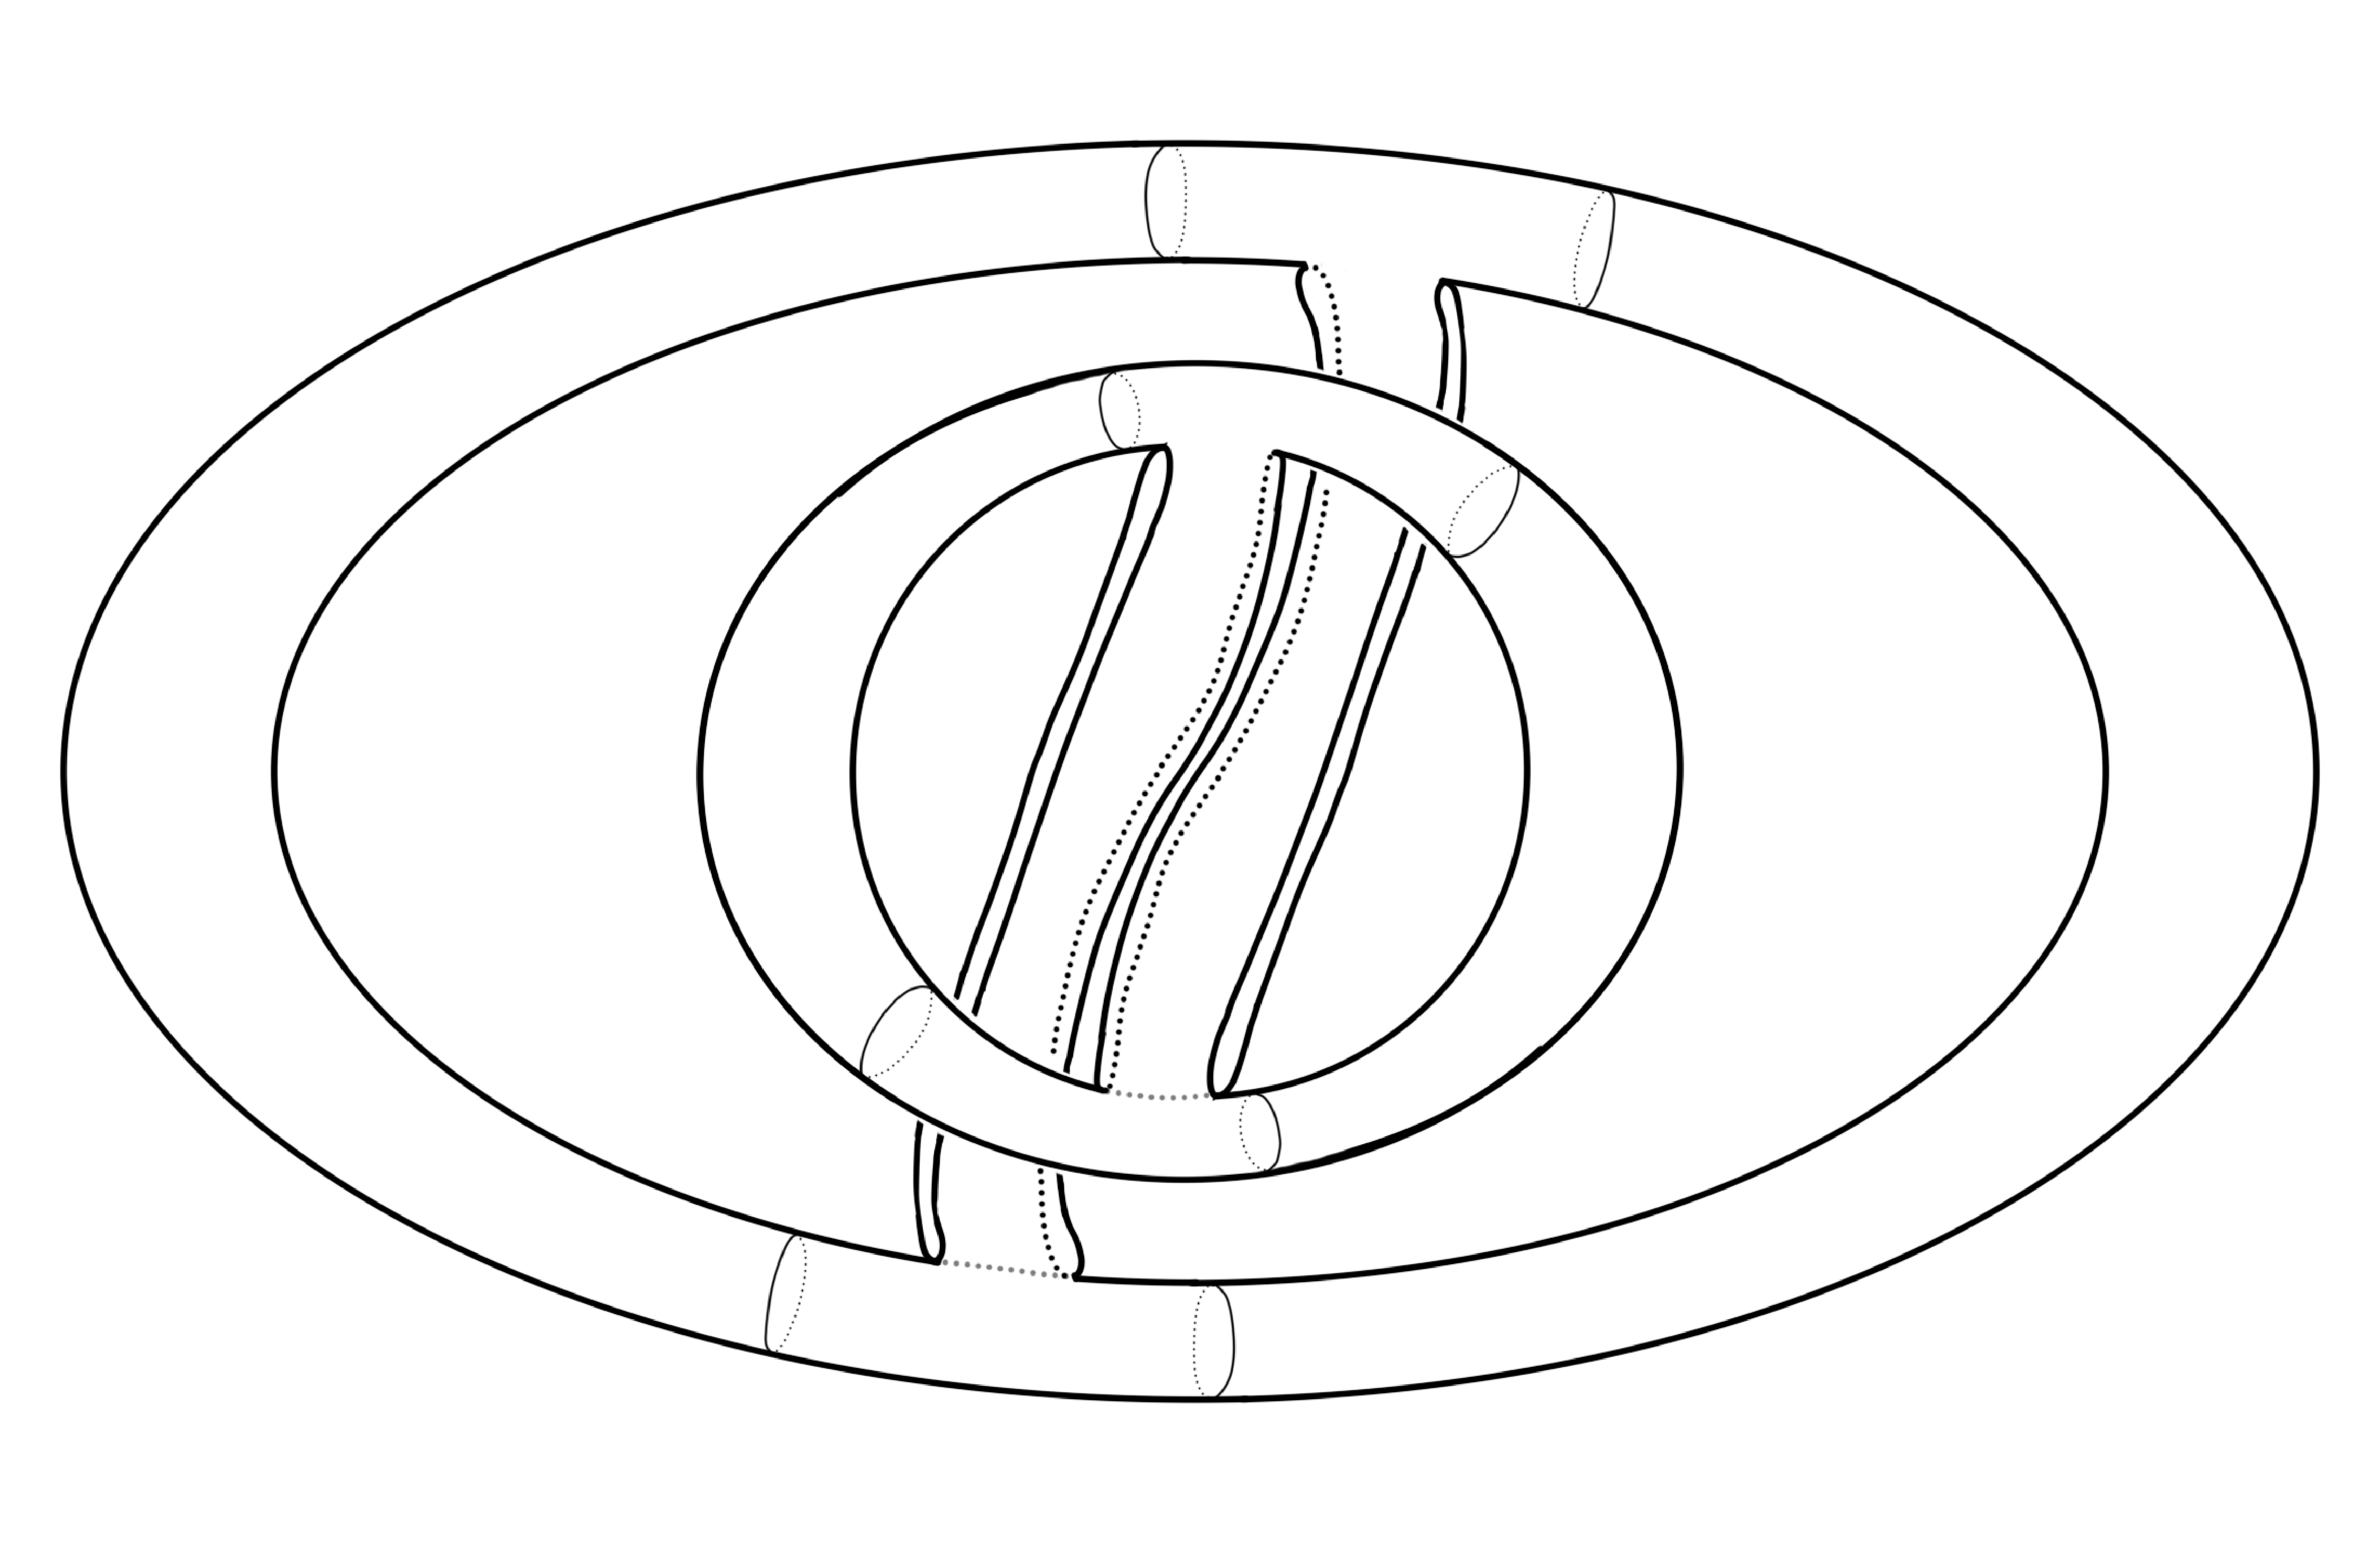
\includegraphics[scale=0.08]{images/ch4/section2/ell_and_hyp2_transformations.pdf}
    \caption{Склейка листов по эллиптическим листам --- это два тора, соединенных лентами.}
    \label{fig:pt9:_ell_and_hyp2_transformations}
\end{figure}
\end{proof}

\subsection{Поверхности уровня для нерегулярных значений интеграла $\Xi$}\label{sec:ch4/sec2/subsec2}
Теперь обратимся к перестройкам поверхностей уровня интеграла $\Xi$. 
Согласно теореме \ref{st:pt9:n1_n2_surfaces}, особые значения соответствуют точкам пересечения координатных линий $\alpha_{out}, \alpha_{in} = b^2, a^2$ с прямой \eqref{eq:L_line}, которая определяется тройкой $(\lambda_1, n_{in}, n_{out})$.
Дополним диаграмму  \ref{fig:pt9:_problemA_subdivisions}, на которой жирными линиями отмечены места, где интеграл $\Xi$ может принимать нерегулярные значения. А именно на рис. \ref{fig:pt9:_diagramPlusIrregular} мы перенумеровали различные варианты перестроек поверхностей уровня интеграла $\Xi$. 
Например, стрелка с номером 2 означает, что прямая \eqref{eq:L_line} пересекает области $D_1^5$ и $D_1^6$ и при росте значения интеграла $\Xi$ при определенном критическом значении пересекает границу $\alpha_{in} = b^2$. Эта перестройка описывается ниже в подразделе \textbf{Перестройка 2}.

\begin{figure}[!htb]
\centering
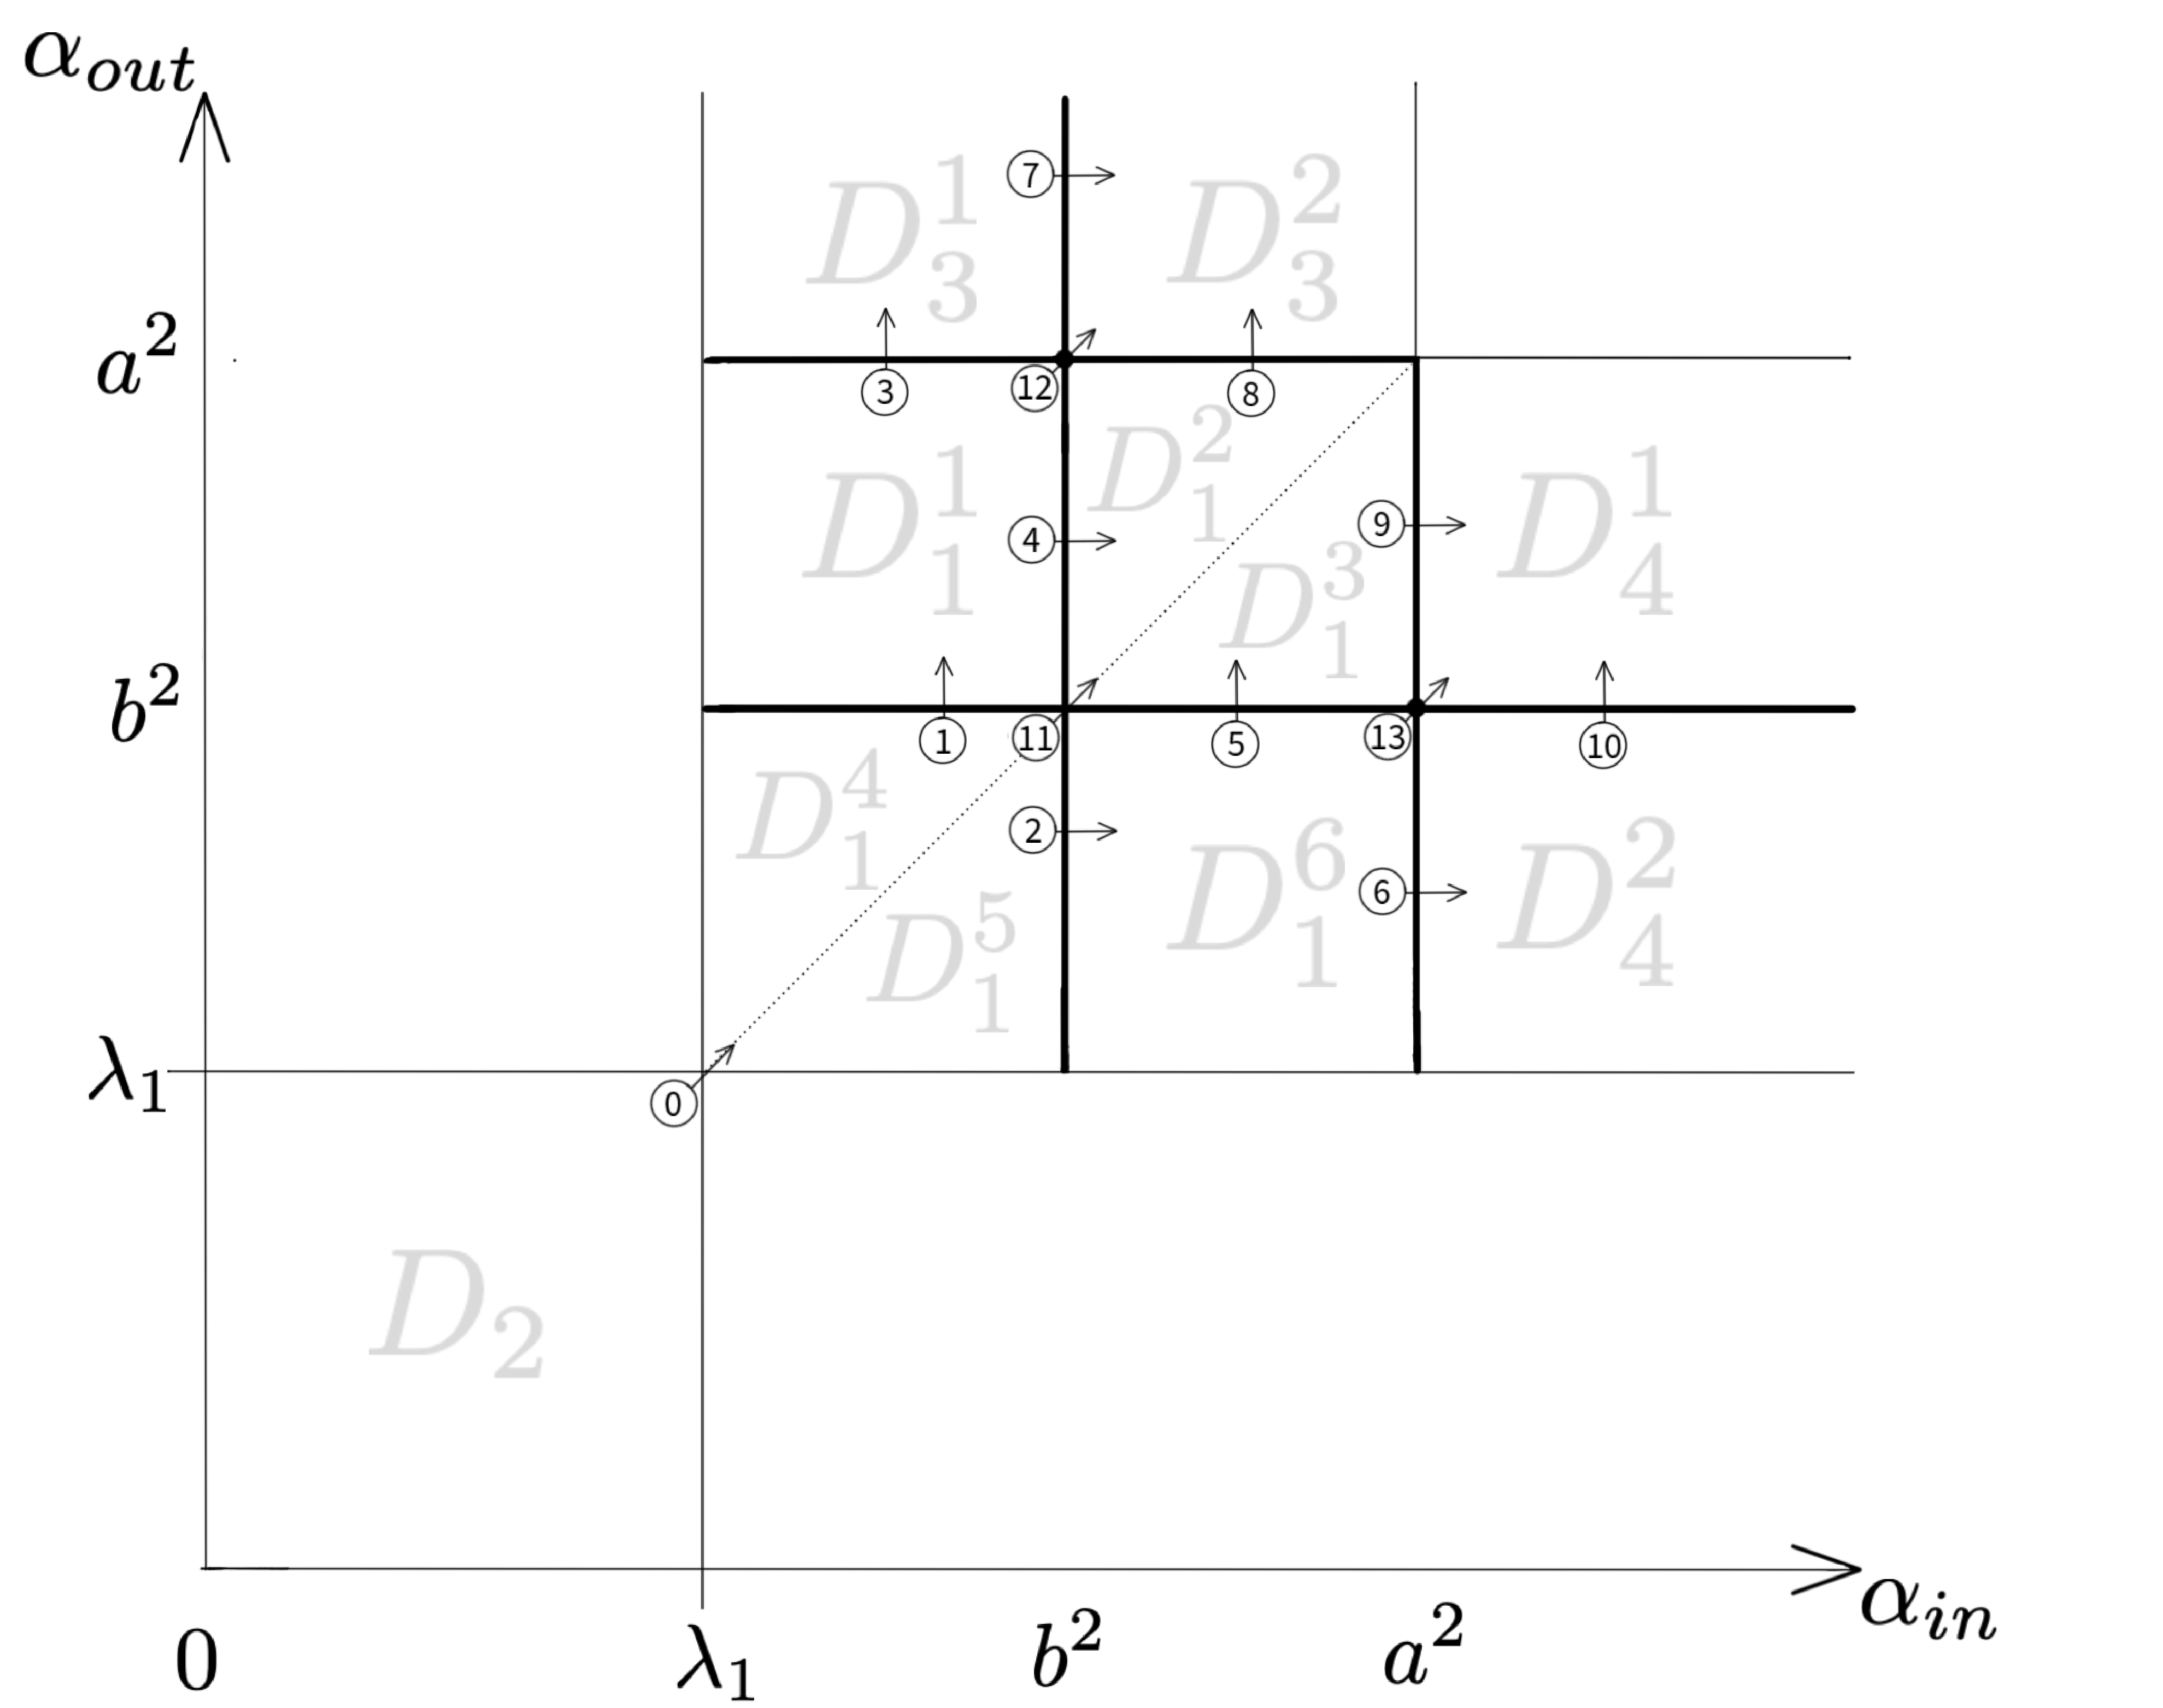
\includegraphics[width=10cm]{images/ch4/section2/diagramPlusIrregular.pdf}
    \caption{Расположение точек, соответствующих нерегулярным значениям $\Xi$.}
    \label{fig:pt9:_diagramPlusIrregular}
\end{figure}

Напомним, что прямая  \eqref{eq:L_line} проходит через точку $(\alpha_{in}, \alpha_{out}) = (\lambda_1, \lambda_1)$ и имеет коэффициент наклона $\dfrac{n_{in}^2}{n_{out}^2}$. Формула \eqref{XiToLine} устанавливает соответствие между значениями интеграла $\Xi$ и точками этой прямой. При возрастании значения интеграла $\Xi$ соответствующая точка на прямой двигается направо вверх. 

\textbf{Перестройка 0} объединяет три случая: переход из $D_2$ в область $D_1^4$, в область $D_1^5$ или на разделяющую их диагональ.
В каждом из этих трех случаев с топологической точки зрения перестройки не происходит: при проходе через особое значение поверхности уровня не меняются (2 тора). 

\textbf{Перестройка 1.} 
Сегменты траектории, находящиеся в области $\Omega_{in}$, касаются эллипса с параметром $\alpha_{in}$. 
В эллиптическом кольце $\Omega_{out}$ звенья траектории лежат на проходящих через фокусы прямых.

Положим $\widetilde{\Omega}_{in} = \Omega_{in} \setminus \Omega_{\alpha_{in}}$. 
В каждой точке $(x,y) \in \Omega_{out} \setminus \{y=0\}$ проекция $\pi$ четырехлистна. Разрежем эллиптическое кольцо вдоль горизонтальной прямой: $\Omega_{out} = \Omega_{out}^u \cup \Omega_{out}^d$, тогда проекция $(x, y, v_x, v_y) \mapsto (x,y)$ будет четырехлистна в каждой внутренней точке любой из полученных областей.
На поверхности $\Xi = \const$ выберем по 4 прообраза для верхней и нижней половины кольца. Обозначим эти прообразы $\Omega_{out, j}^u, \Omega_{out, j}^d, j=1, \ldots, 4$, где нумерацию определим согласно следующему правилу:
\begin{equation}
\begin{array}{ll}
1: & \text{ вектор } (v_x, v_y) \text{ направлен к правому фокусу }, \\
2: & \text{ вектор } (v_x, v_y) \text{ направлен к левому фокусу }, \\
3: & \text{ вектор } (v_x, v_y) \text{ направлен от правого фокуса }, \\
4: & \text{ вектор } (v_x, v_y) \text{ направлен от левого фокуса}.
\end{array}
\label{eq:foc_numeration}
\end{equation}
При этом прообразы  $\widetilde{\Omega}_{in, j}, j=1, \ldots, 4$ занумерованы в соответствии с правилом \eqref{eq:ell_numeration}.

Области $\Omega_{out, j}^u$ и $\widetilde{\Omega}_{in, j}$ для каждого $j=1, \ldots, 4$ отождествляются по общей границе в соответствии с законом преломления $(\ast)$; общая граница указанных областей проецируется в дугу эллипса $Q_{\lambda_1} \cap \{y > 0\}$. 
В симметричную ей дугу в нижней полуплоскости отображается общая для областей $\widetilde{\Omega}_{in, 1}$ и $\Omega_{out, 2}^d$ граница на поверхности $\Xi = \const$. Аналогично отождествляются области $\widetilde{\Omega}_{in, 2}$ и $\Omega_{out, 1}^d$, $\widetilde{\Omega}_{in, 3}$ и $\Omega_{out, 4}^d$, а также $\widetilde{\Omega}_{in, 4}$ и $\Omega_{out, 3}^d$.

Отметим, что горизонтальная прямая пересекается с кольцом $\Omega_{out}$ по двум отрезкам $I_1$ и $I_2$. На каждый из них проецируются общие границы для четверок областей: $\Omega_{out, 1}^u, \Omega_{out, 1}^d, \Omega_{out, 2}^u, \Omega_{out, 2}^d$. Аналогично для областей $\Omega_{out, 3}^u, \Omega_{out, 3}^d$, $ \Omega_{out, 4}^u, \Omega_{out, 4}^d$.

Определим области $\widetilde{\Omega}_1 = \Omega_{out, 1}^u \cup \widetilde{\Omega}_{in, 1} \cup \Omega_{out, 2}^d$, $\widetilde{\Omega}_2 = \Omega_{out, 2}^u \cup \widetilde{\Omega}_{in, 2} \cup \Omega_{out, 1}^d$, аналогично определим области $\widetilde{\Omega}_3 = \Omega_{out, 3}^u \cup \widetilde{\Omega}_{in, 3} \cup \Omega_{out, 4}^d$ и $\widetilde{\Omega}_4 = \Omega_{out, 4}^u \cup \widetilde{\Omega}_{in, 4} \cup \Omega_{out, 3}^d$. Пример области $\widetilde{\Omega}_1$ см. рис. \ref{fig:pt9:_domain_atom_ell_foc},  жирным пунктиром  изображен отрезок, проецирующийся в  $I_1$, а жирным сплошным --- проецирующийся в $I_2$.

\begin{figure}[!htb]
\minipage{0.43\textwidth}
\centering
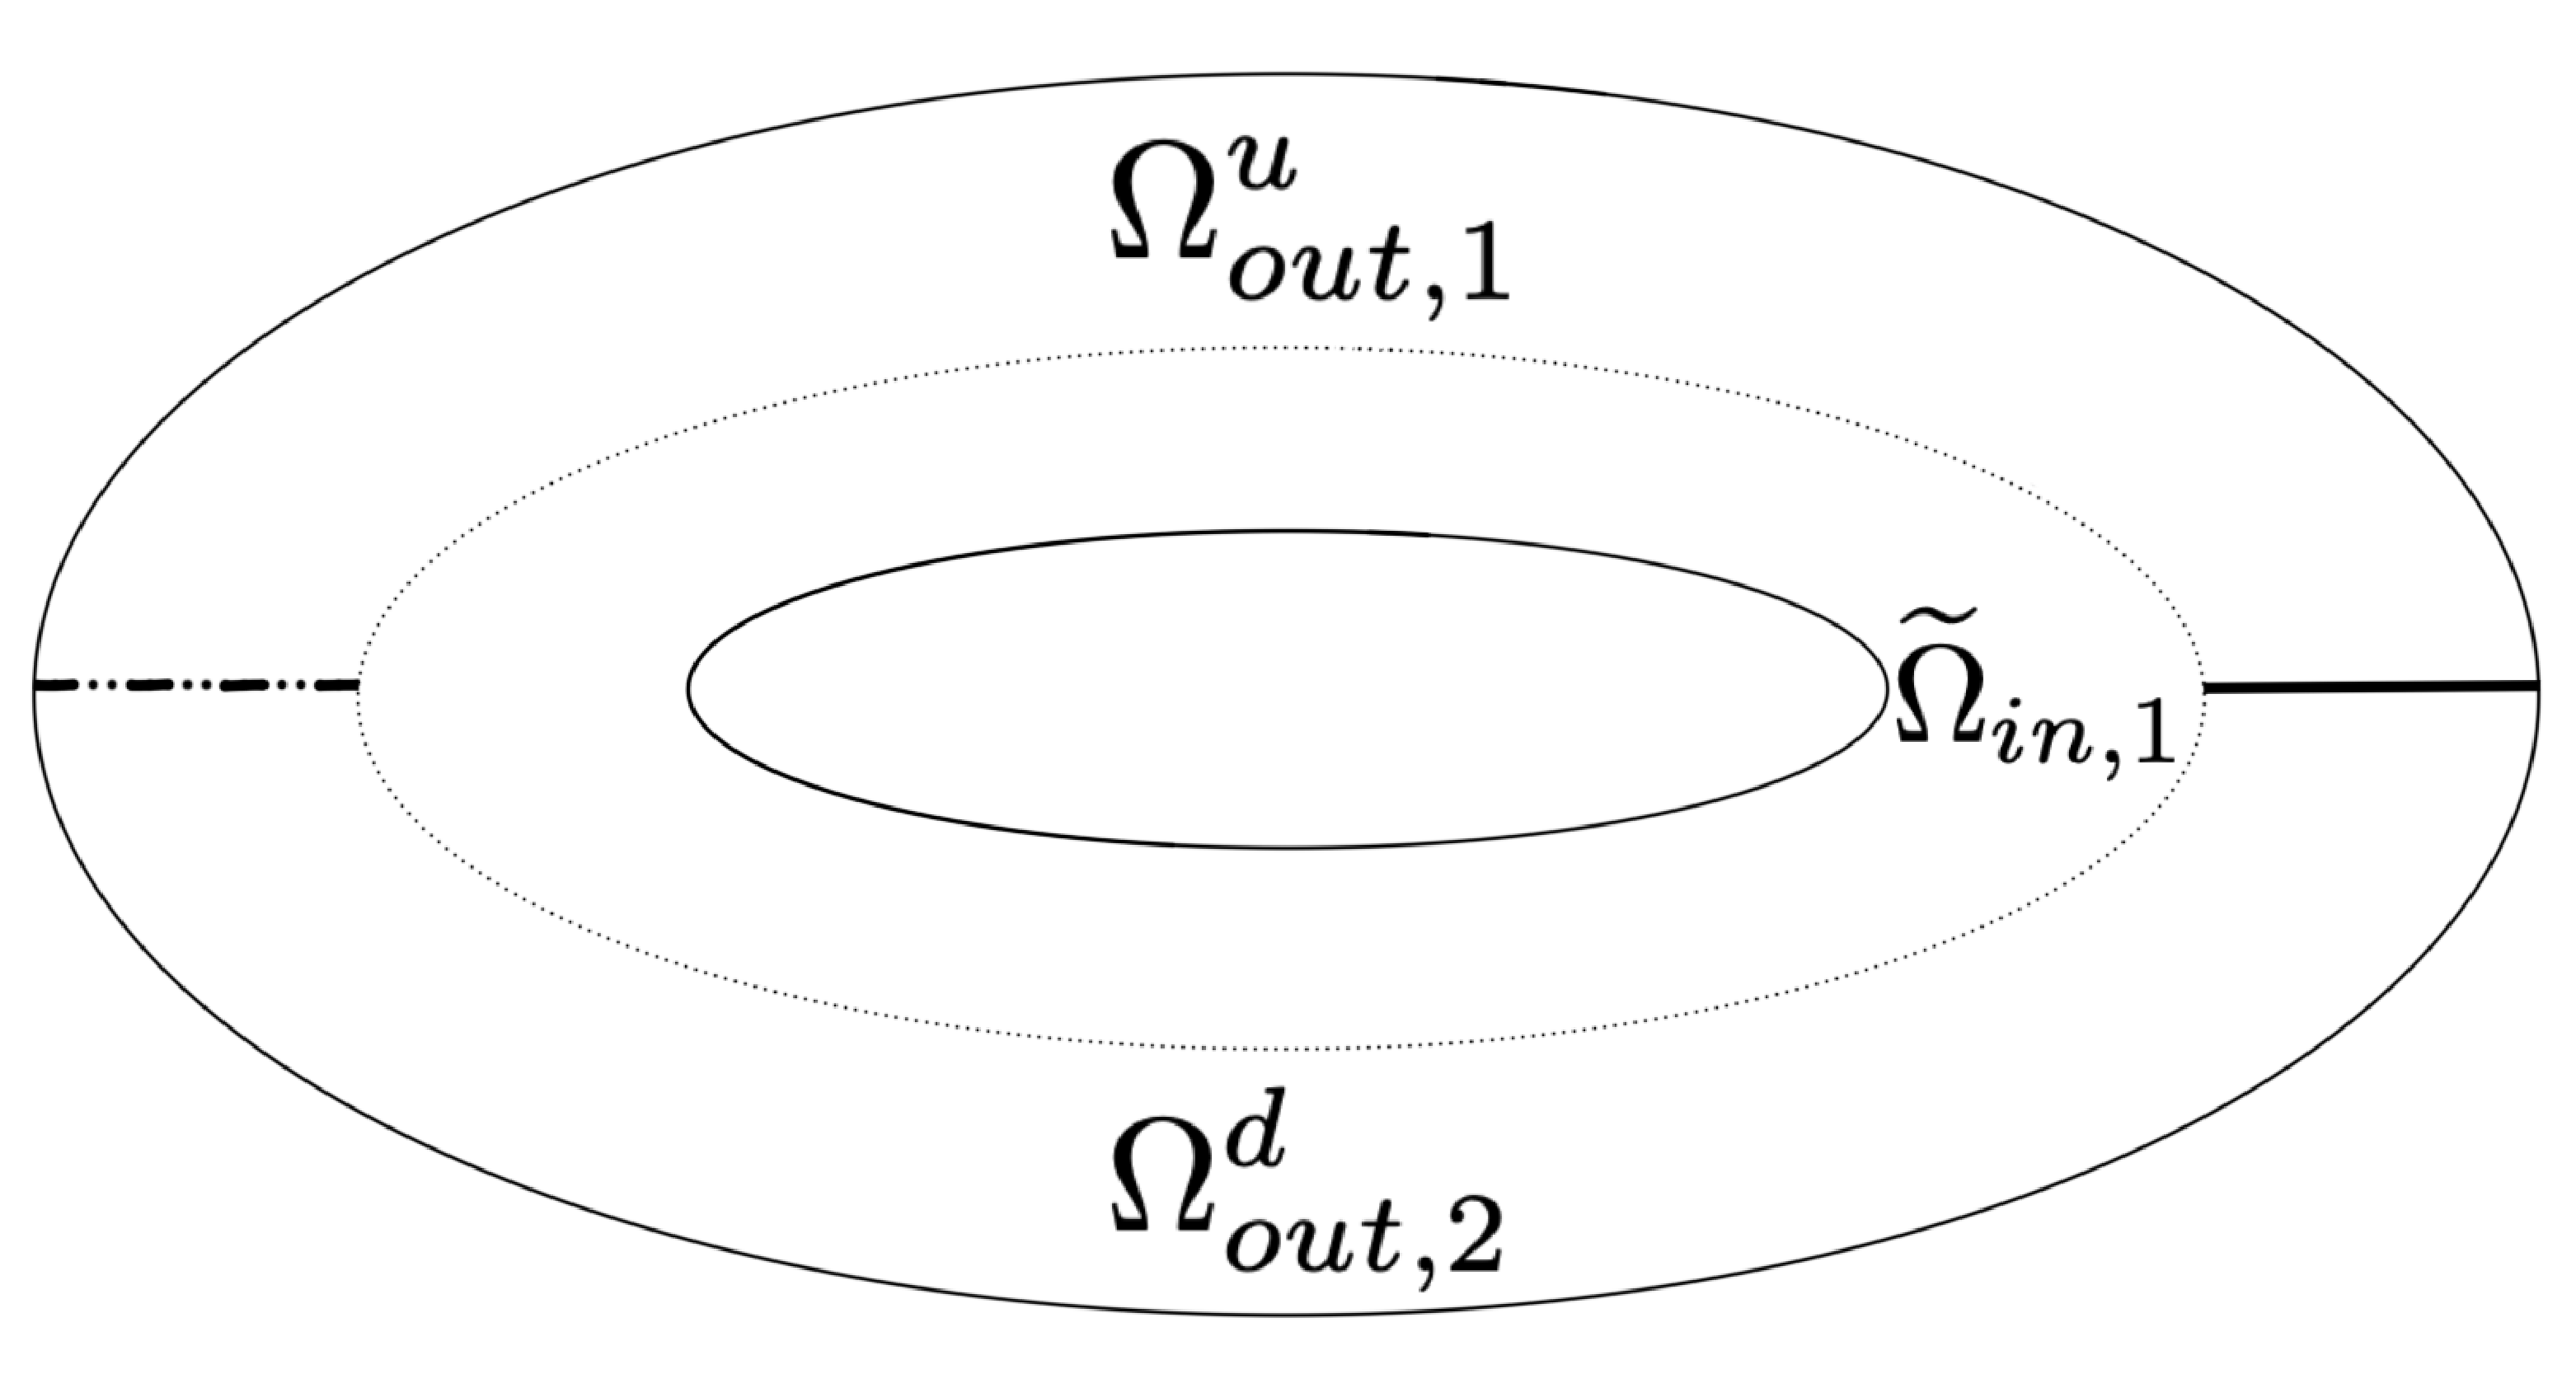
\includegraphics[scale=0.125]{images/ch4/section2/atoms/domain_atom_ell_foc.pdf}
    \caption{Пример области $\widetilde{\Omega}_1$ для перестройки 1.}
    \label{fig:pt9:_domain_atom_ell_foc}
\endminipage\hfill
\minipage{0.42\textwidth}
\centering
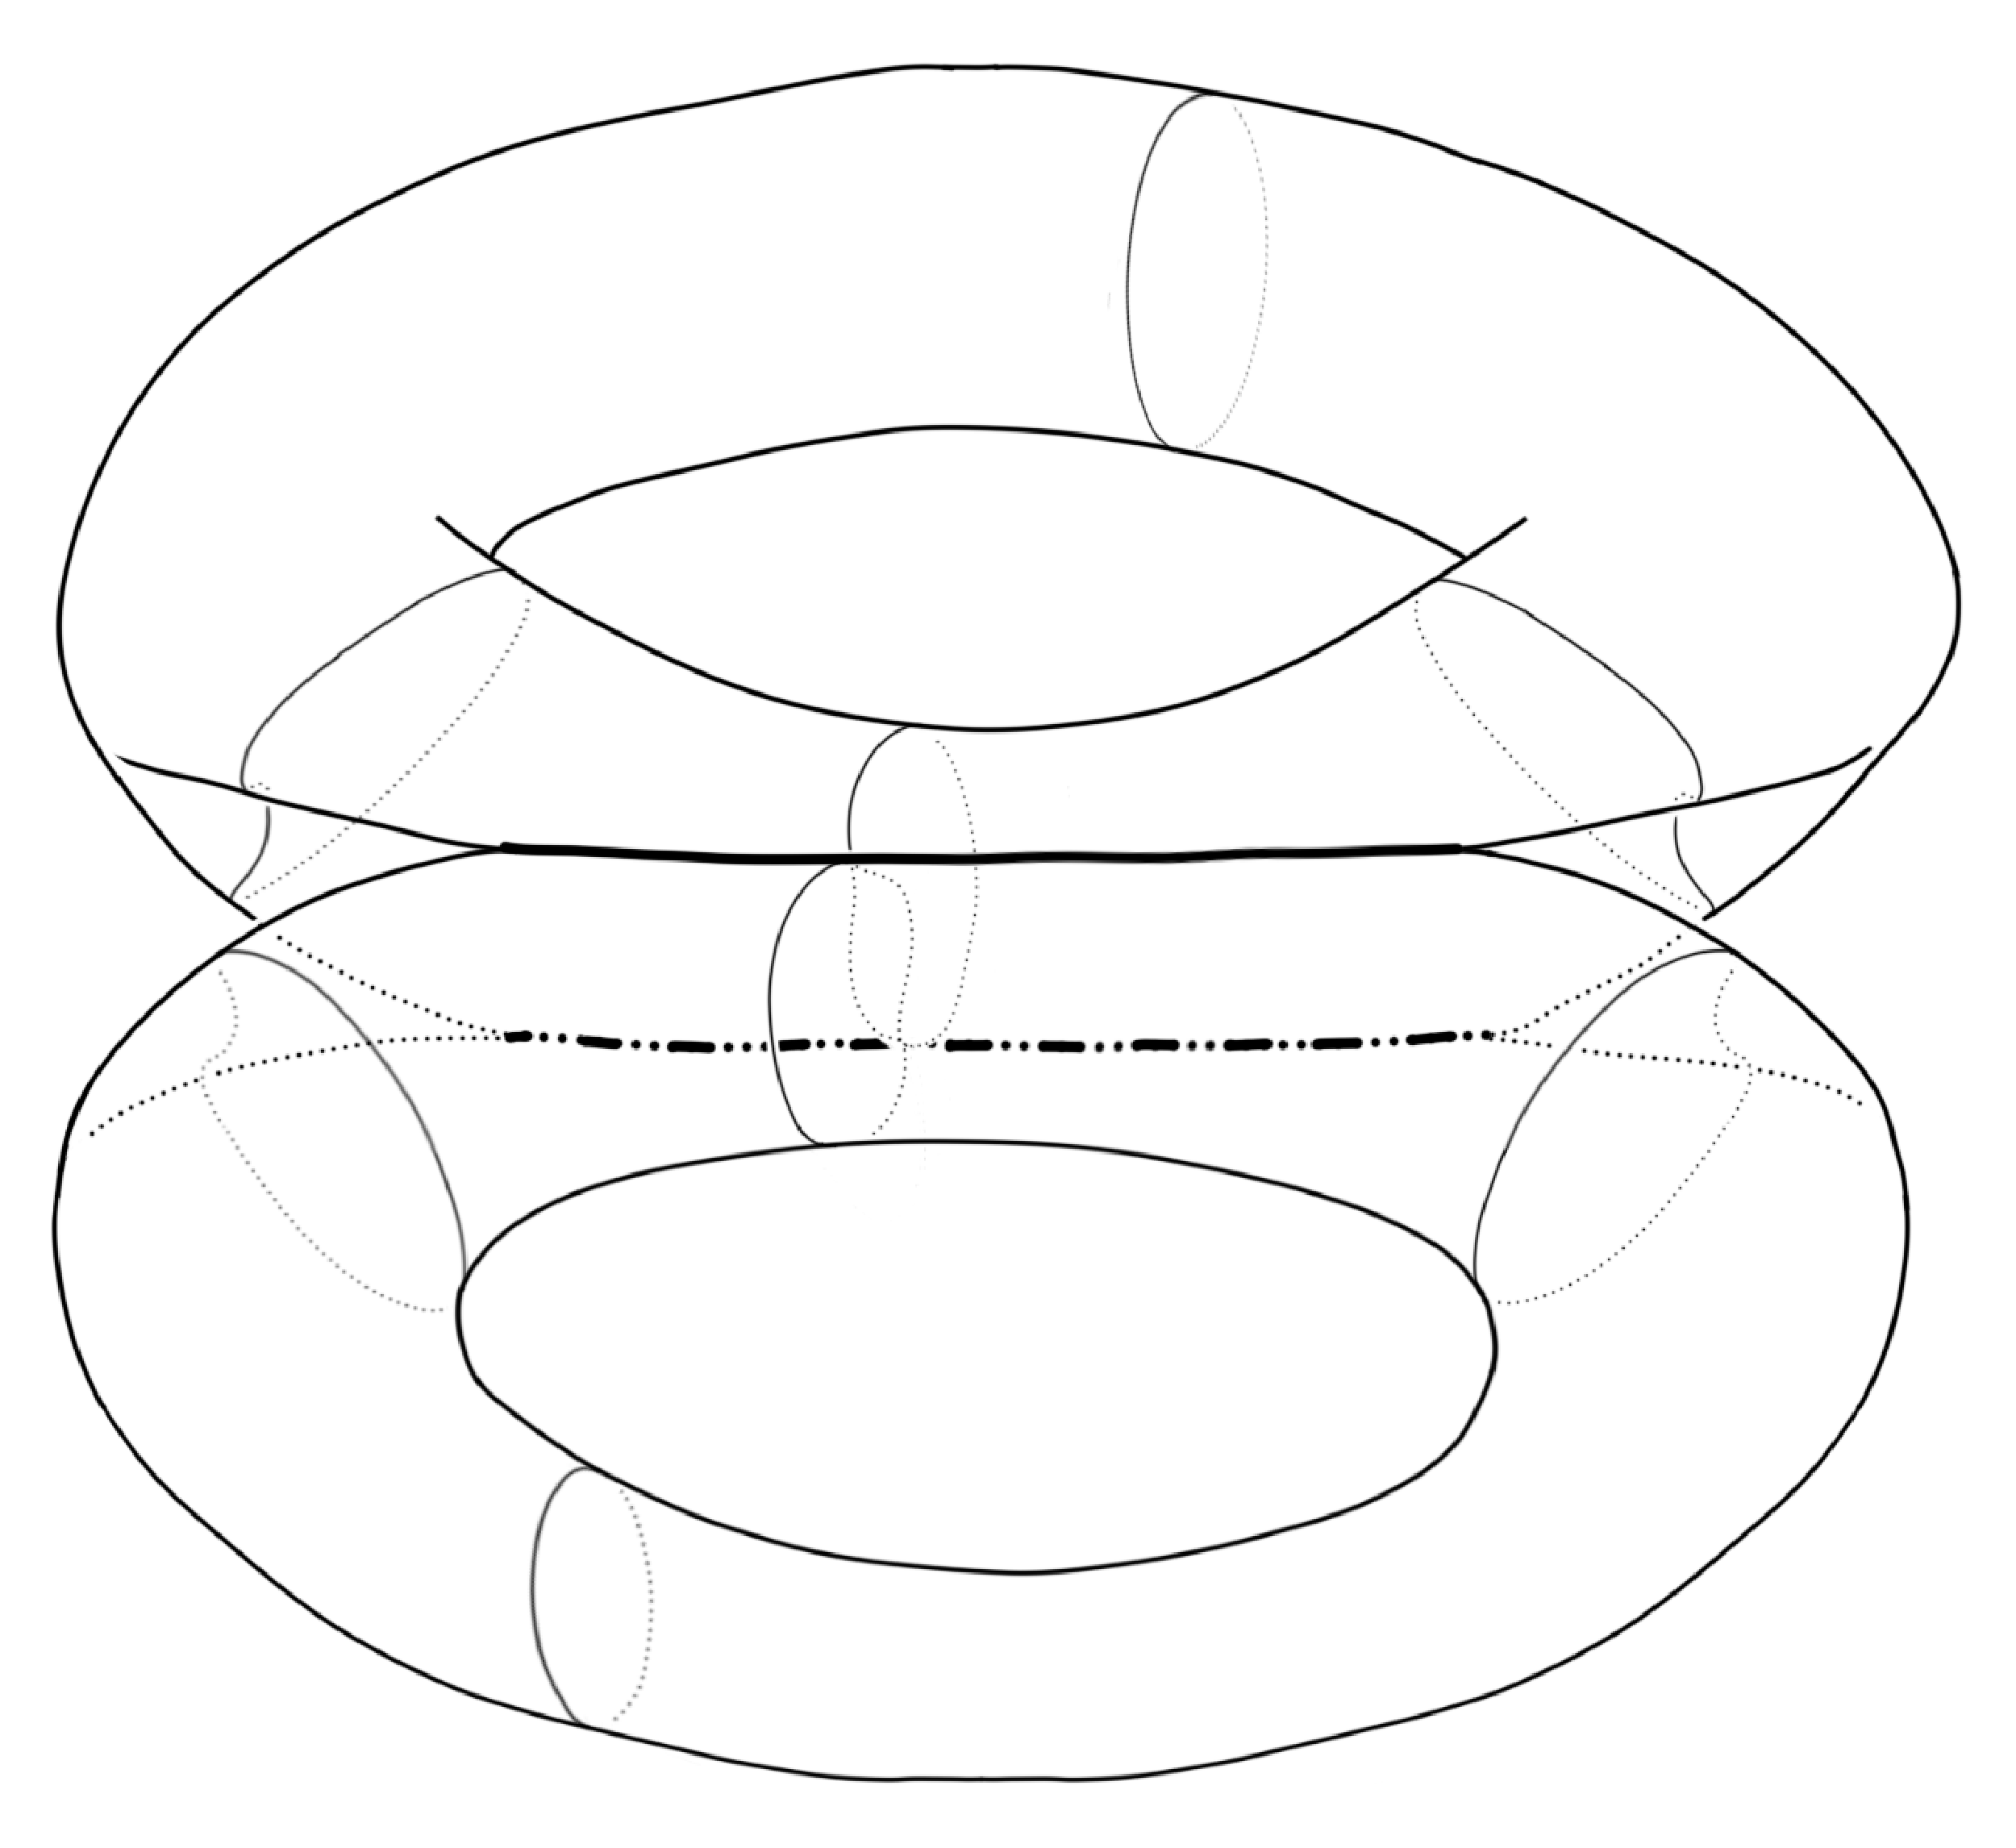
\includegraphics[scale=0.125]{images/ch4/section2/atoms/atom1_result.pdf}
    \caption{Поверхность уровня $\Xi=\const$ для перестройки 1.}
    \label{fig:pt9:_atom1_result}
\endminipage\hfill
\end{figure}


Склеим области $\widetilde{\Omega}_1$ и $\widetilde{\Omega}_4$ по одноименным эллиптическим границам, получим один тор. Аналогично для областей $\widetilde{\Omega}_2$ и $\widetilde{\Omega}_3$.

При этом на торе $\widetilde{\Omega}_1 \cup \widetilde{\Omega}_4$ в одной конечной точке отождествляются два прообраза пунктирного  отрезка $I_1$, аналогично для сплошного отрезка $I_2$. На  торе $\widetilde{\Omega}_2 \cup \widetilde{\Omega}_3$ также присутствуют кривые, двулистно накрывающие отрезки $I_1$ и  $I_2$.
На рис. \ref{fig:pt9:_atom1_result} кривые изображены жирным и пунктиром.
Остается отождествить два тора по этим кривым, тогда поверхность уровня $\Xi = \const$ представляет собой склейку двух торов по двум конечным отрезкам (см. рис. \ref{fig:pt9:_atom1_result}). 


\textbf{Перестройка 2.} 
Сегменты бильярдной траектории в области $\Omega_{in}$ лежат на прямых, проходящих через фокусы, а продолжения звеньев траектории в кольце $\Omega_{out}$ касаются эллипса с параметром $\alpha_{out}$. 

Проекция поверхности $\Xi = \const$ заметает всю область $\Omega$. При этом каждой внутренней точке $\Omega_{out} \cup (\Omega_{in} \setminus \{y=0\})$ соответствует четыре точки на поверхности.
Разрежем область $\Omega$ по горизонтальной прямой и представим  ее в виде объединения $\Omega_{out}^u \cup \Omega_{in}^u \cup \Omega_{in}^d \cup \Omega_{out}^d$. 
Каждой из указанных областей соответствует по четыре области на поверхности $\Xi = \const$, обозначим их $\Omega_{out, j}^u , \Omega_{in, j}^u , \Omega_{in, j}^d , \Omega_{out, j}^d, j=1, \ldots, 4$. 
При этом для прообразов $\Omega_{out, j}^u$ и $\Omega_{out, j}^d$ используем нумерацию в соответствии с правилом \eqref{eq:ell_numeration}. 
Прообразы $\Omega_{in, j}^u$ и $\Omega_{in, j}^d$ пронумерованы как в правиле \eqref{eq:foc_numeration}.

Заметим, что на поверхности $\Xi = \const$ области $\Omega_{out, j}^u$ и $\Omega_{in, j}^u$ отождествляются по общей границе, которая проектируется в дугу эллипса $Q_{\lambda_1} \cap \{ y > 0\}$, где $j=1, \ldots,4$. Обозначим $\Omega_j^u = \Omega_{out, j}^u \cup \Omega_{in, j}^u, j=1, \ldots, 4$.

В симметричную дугу в нижней полуплоскости проектируется общий сегмент границ областей $\Omega_{in, 1}^d$ и $\Omega_{out, 3}^d$, на котором эти области отождествляются. 
%Обозначим результат их склейки как $\Omega_3^d$. 
%Аналогично определим $\Omega_1^d = \Omega_{in, 2}^d \cup \Omega_{out, 1}^d$, а также $\Omega_2^d = \Omega_{in, 1}^d \cup \Omega_{out, 2}^d$ и $\Omega_4^d = \Omega_{in, 3}^d \cup \Omega_{out, 4}^d$.
Аналогично  отождествляются $\Omega_{in, 2}^d$ c $\Omega_{out, 1}^d$, а также $\Omega_{in, 1}^d$ c $\Omega_{out, 2}^d$ и $\Omega_{in, 3}^d$ с $ \Omega_{out, 4}^d$.

На горизонтальной оси можно выделить пять сегментов: два из них попадают в $\Omega_{out}$ и три в $\Omega_{in}$, один из которых соединяет фокусы.
В отрезок между фокусов проектируется общая граница для четырех областей $\Omega_1^u, \Omega_4^u, \Omega_{in, 1}^d$ и $\Omega_{in, 4}^d$.
Аналогично общая граница областей $\Omega_2^u, \Omega_3^u, \Omega_{in, 2}^d$ и $\Omega_{in, 3}^d$ проектируется на этот же отрезок.

Определим области 
\begin{equation}
\begin{array}{cc}
\widetilde{\Omega}_1 = \Omega_1^u \cup \Omega_{in, 4}^d \cup \Omega_{out, 3}^d, &
\widetilde{\Omega}_2 = \Omega_2^u \cup \Omega_{in, 3}^d \cup \Omega_{out, 4}^d, \\
\widetilde{\Omega}_3 = \Omega_3^u \cup \Omega_{in, 2}^d \cup \Omega_{out, 1}^d, &
\widetilde{\Omega}_4 = \Omega_4^u \cup \Omega_{in, 1}^d \cup \Omega_{out, 2}^d. 
\end{array}
\label{eq:case2Omegas}
\end{equation}
Пример области $\widetilde{\Omega}_1$ изображен на рис. \ref{fig:pt9:_domain_atom_foc_ell}.
 \begin{figure}[!htb]
\centering
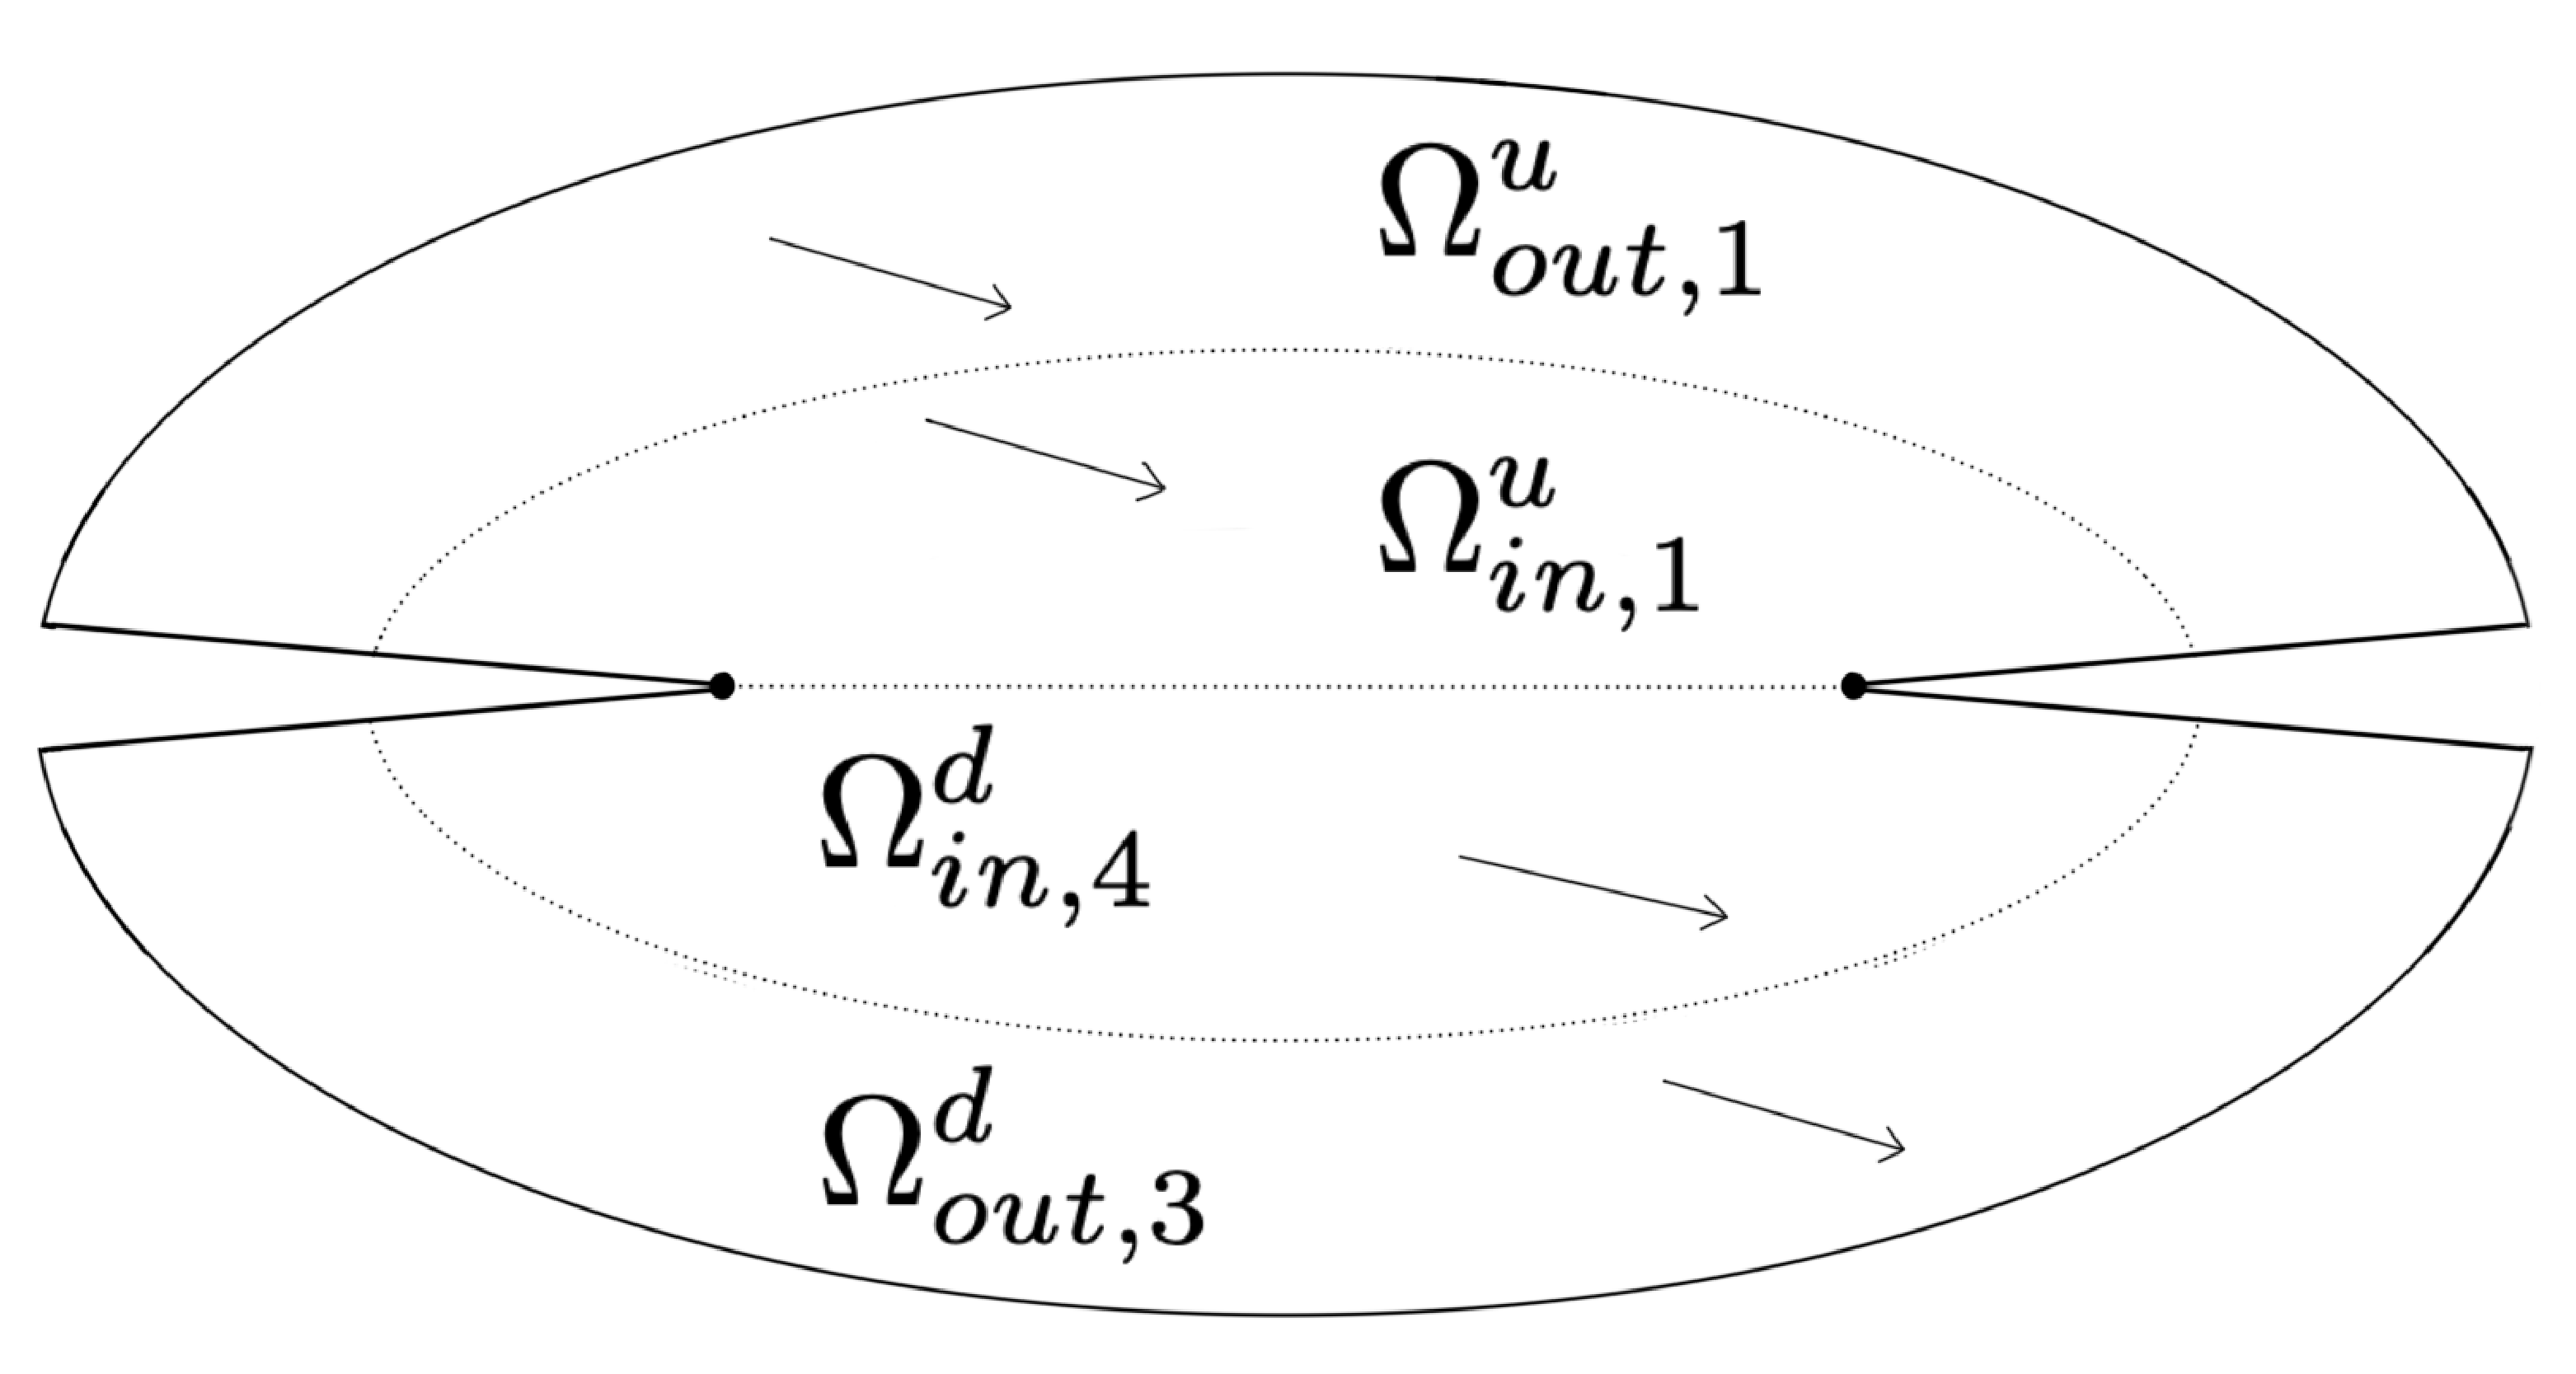
\includegraphics[scale=0.125]{images/ch4/section2/atoms/domain_atom_foc_ell.pdf}
    \caption{Пример области $\widetilde{\Omega}_1$ для перестройки 2.}
    \label{fig:pt9:_domain_atom_foc_ell}
\end{figure}
 
Склеим области $\widetilde{\Omega}_1$ и $\widetilde{\Omega}_4$ по граничным эллиптическим дугам, а также по прообразу соединяющего фокусы отрезка на $\Xi = \const$. Аналогично для областей $\widetilde{\Omega}_2$ и $\widetilde{\Omega}_3$. Получим два цилиндра; поперечное сечение каждого даст восьмерку. 

Рассмотрим прообраз на $\Xi = \const$ горизонтального отрезка, левый конец которого находится в правом фокусе, а правый --- в правой вершине $Q_{\lambda_1}$.
В этот сегмент прямой, в силу изложенных в \cite[\S 4]{Fok15} соображений, проектируется общая граница для областей $\Omega_{in, 1}^u$ и $\Omega_{in, 2}^d$. Аналогично для пар областей $\Omega_{in, 2}^u$ и $\Omega_{in, 1}^d$, $\Omega_{in, 3}^u$ и $\Omega_{in, 4}^d$ и для пары $\Omega_{in, 4}^u$ и $\Omega_{in, 3}^d$. 
То есть на поверхности $\Xi = \const$ (см. \eqref{eq:case2Omegas}) \textit{верхняя} граница области $\widetilde{\Omega}_1$ отождествляется с \textit{нижней} границей области $\widetilde{\Omega}_3$ и наоборот. Аналогично для двух других областей: \textit{верхняя} граница $\widetilde{\Omega}_2$ --- с \textit{нижней} границей области $\widetilde{\Omega}_4$ и наоборот. 
Из аналогичных соображений следуют такие же склейки на прообразе симметричного отрезка, соединяющем левую вершину эллипса $Q_{\lambda_1}$ и левый фокус.

Рассмотрим отрезки $\Omega_{out} \cap \{y=0\}$. 
На каждый из них проектируются общие границы областей $\Omega_{out, j}^u$ и $\Omega_{out, j}^d$ для $j=1, \ldots, 4$. 
То есть, по прообразу каждого из отрезков отождествляются листы (см. \eqref{eq:case2Omegas}) $\widetilde{\Omega}_1$ с $\widetilde{\Omega}_3$, а также $\widetilde{\Omega}_2$ с  $\widetilde{\Omega}_4$.
% Поскольку склейки отрезков идентичны тем, что были получены в предыдущем абзаце, будем считать их одной склейкой.

Склеим листы $\widetilde{\Omega}_1$ с $\widetilde{\Omega}_4$ по трем общим дугам и получим два соединенных вдоль общей горизонтальной прямой цилиндра (или, что то же самое, цилиндр с восьмеркой в сечении). Аналогично склеим листы $\widetilde{\Omega}_2$ и $\widetilde{\Omega}_3$.
При этом две дуги, ограничивающие левую окружность верхнего цилиндра $\widetilde{\Omega}_1 \cup \widetilde{\Omega}_4$, проектируются в отрезок горизонтальной прямой, соединяющий левую вершину граничного эллипса с левым фокусом. В этот же отрезок проецируются дуги, ограничивающие левую окружность правого цилиндра  $\widetilde{\Omega}_1 \cup \widetilde{\Omega}_4$. Аналогично для $\widetilde{\Omega}_2$ и $\widetilde{\Omega}_3$. То же самое справедливо для дуг, ограничивающих правые окружности цилиндров, только проецируются они на симметричный горизонтальный отрезок от правого фокуса к правой вершине граничного эллипса.
Остается склеить цилиндры между собой: левая окружность \textit{верхнего} цилиндра $\widetilde{\Omega}_1 \cup \widetilde{\Omega}_4$ отождествляется с левой окружностью \textit{нижнего} цилиндра $\widetilde{\Omega}_2 \cup \widetilde{\Omega}_3$, а левая окружность \textit{нижнего} цилиндра $\widetilde{\Omega}_1 \cup \widetilde{\Omega}_4$ --- с левой окружностью \textit{верхнего} цилиндра $\widetilde{\Omega}_2 \cup \widetilde{\Omega}_3$. 
Аналогичные склейки возникают на правых окружностях цилиндров. 

Таким образом, поверхность $\Xi = \const$ представляет собой тор с восьмеркой в продольном сечении, см. рис. \ref{fig:pt9:_foc_ell_atom}.
\begin{figure}[!htb]
\centering
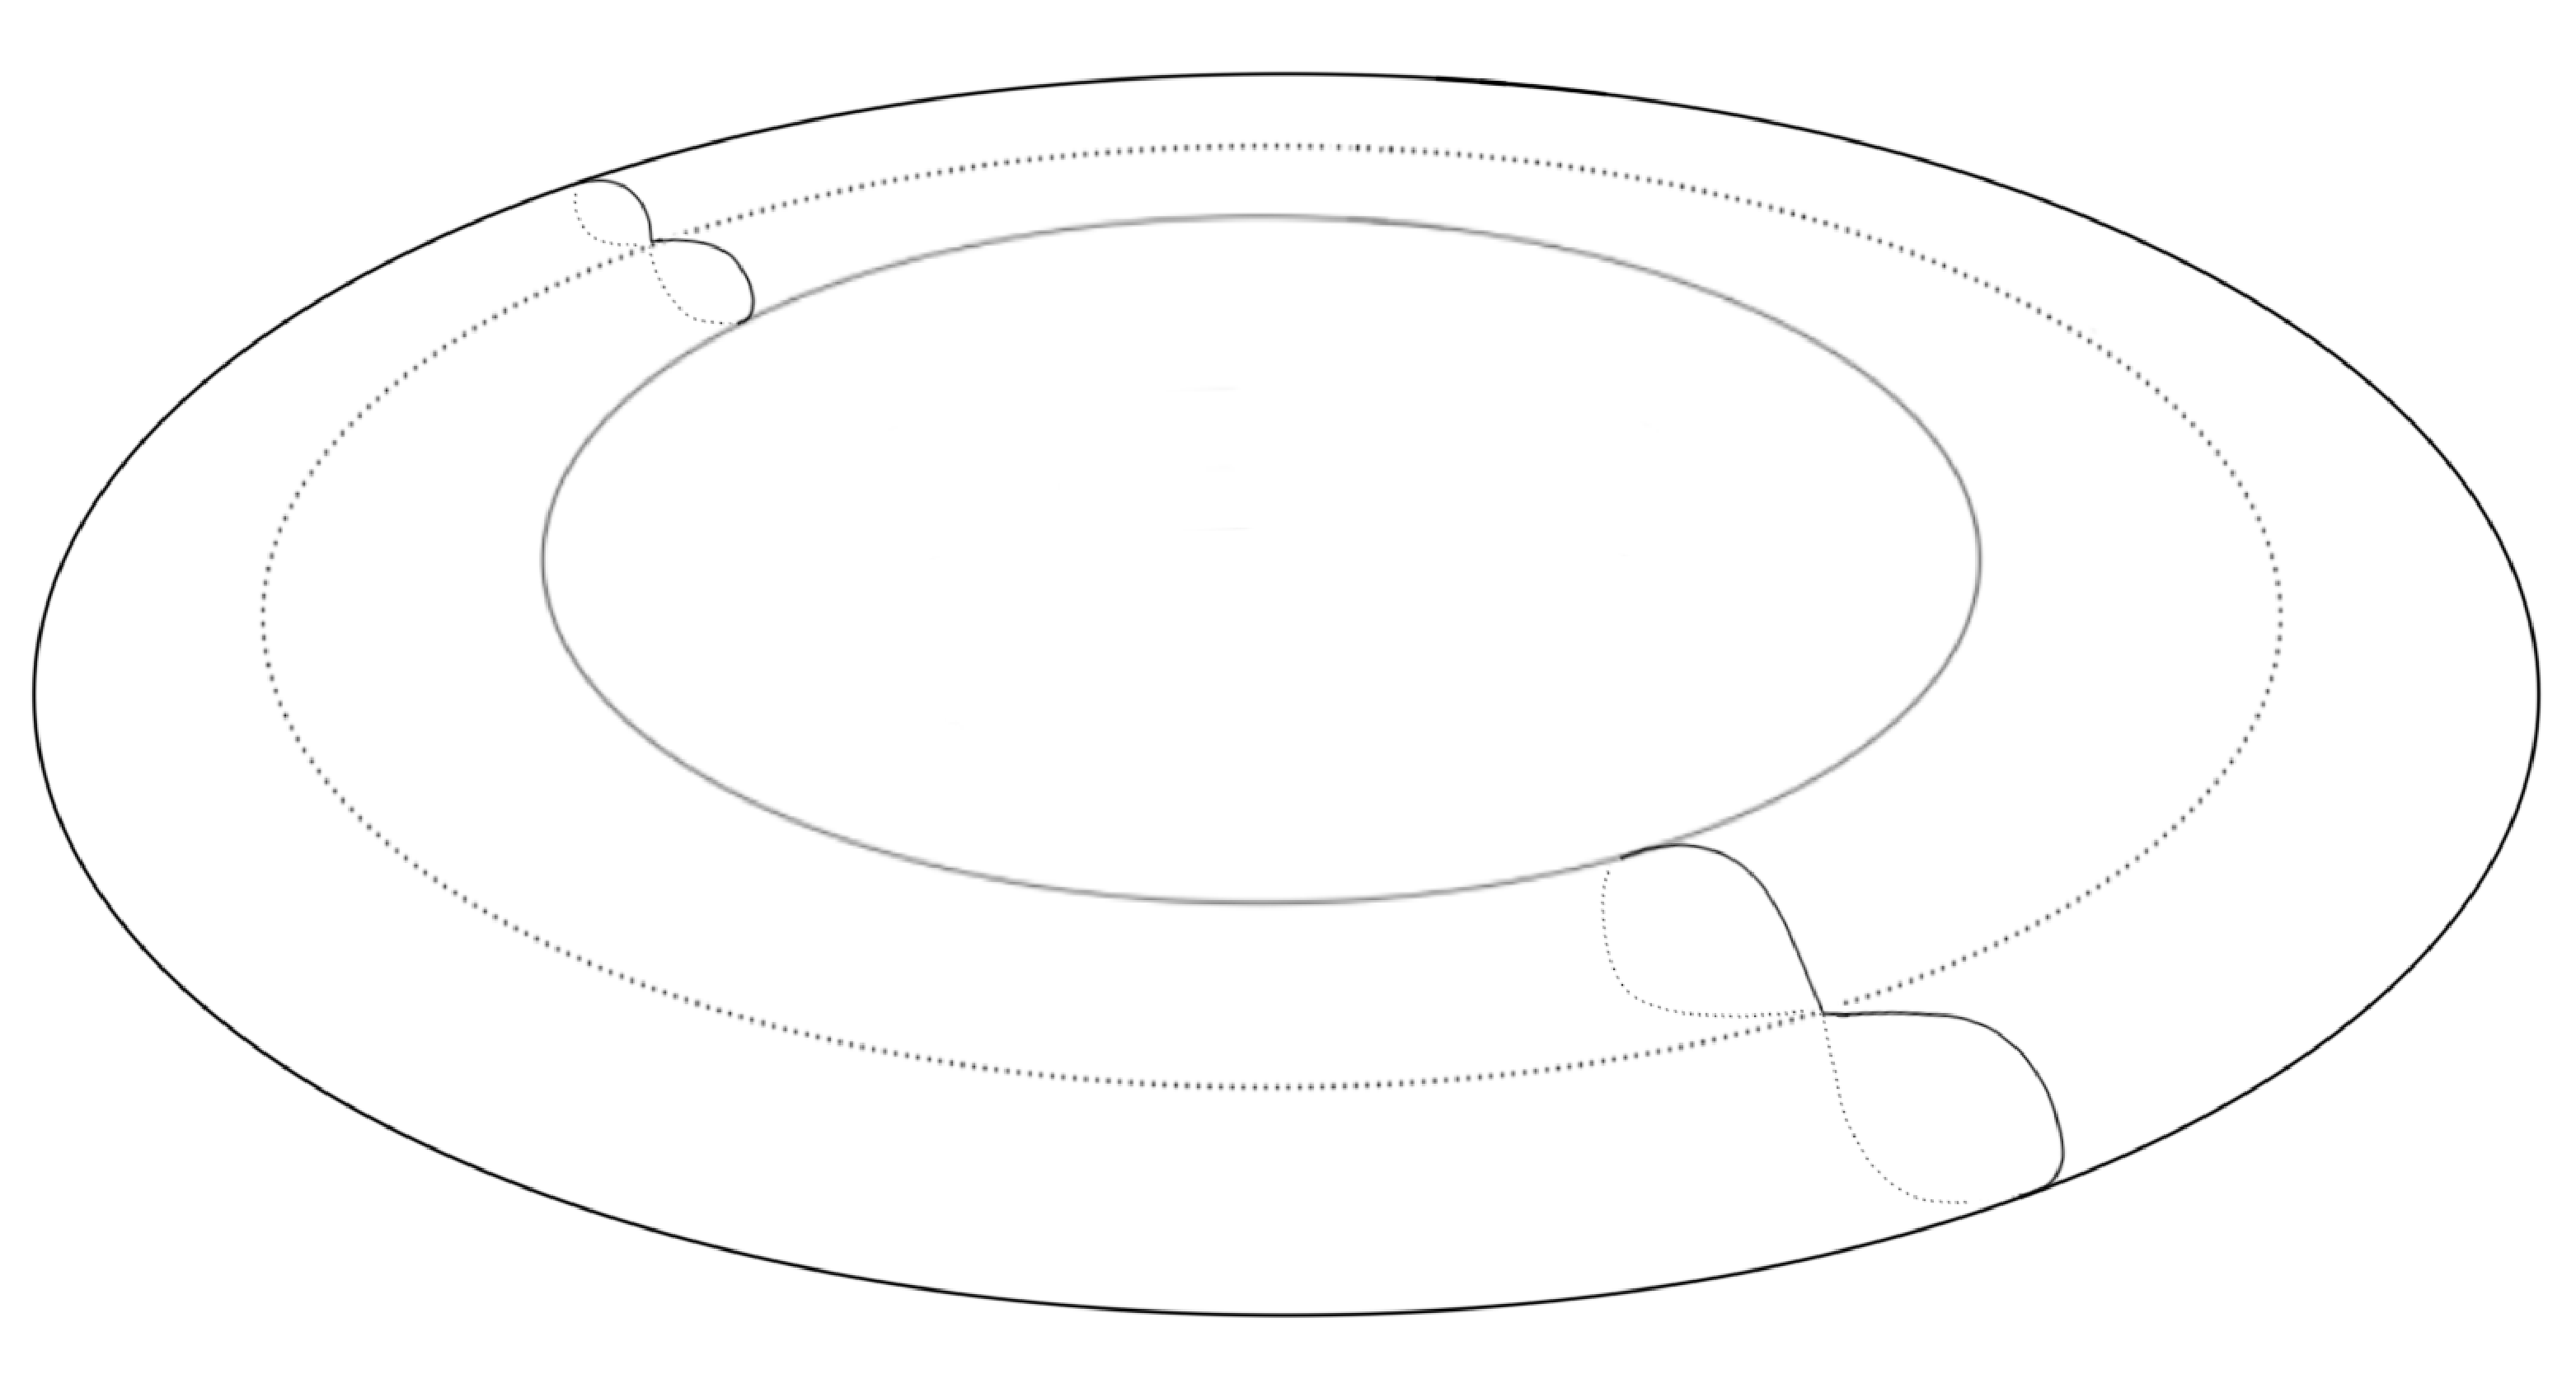
\includegraphics[scale=0.125]{images/ch4/section2/atoms/foc_ell_atom.pdf}
\caption{Поверхность уровня $\Xi = \const$ для перестройки 2.}
\label{fig:pt9:_foc_ell_atom}
\end{figure}

% \textcolor{red}{векторы в нижнем внутреннем эллипссе в \ref{fig:pt9:_domain_atom_foc_ell} определены неправильно. ВСЕ ПЕРЕДЕЛАТЬ}
 
%Соответствует случаю $\alpha_{in} = b^2, \ \alpha_{out} \in (\lambda_1, b^2)$.
%В этом случае каустика траектории во внешнем кольце $\Omega_{out}$ является эллипсом, а во внутренней области $\Omega_{in}$ интегральные траектории проходят вдоль прямых, которые содержат один из фокусов. 
%Векторы скоростей в области $\Omega_{in}$ и  $\Omega_{out}$ определим так же ранее (см. Рис. \ref{fig:pt9:_domain_atom_foc_ell}). 
%
%%При этом часть соединяющей фокусы прямой, которая попала в область $\Omega_{in}$, также рассмотрим как предельный случай софокусной гиперболы с устремленным к $b^2$ сверху параметром (см. Рис. \ref{fig:pt9:_atom1_result}). 
%Разрежем каждый лист $(\Omega, v_i), i=1,\ldots, 4$ вдоль горизонтальных пунктирных линий, соответствующих вырожденным гиперболам. 
%При этом разрез проходит в том числе через $\Omega_{out}$. 
%Пример листа склейки изображен на Рис. \ref{fig:pt9:_atom_foc_ell_leaf}.
%На Рис. \ref{fig:pt9:_atom_foc_ell_iter1}  изображен результат склейки листов $(\Omega, v_1)$ (на заднем плане) и $(\Omega, v_4)$ (на переднем плане). 
%Завершающие граничные восьмерки дуги склеиваются попарно, верхняя с нижней, по склейкам $\alpha$ и $\beta$. 
%Склейка листов $(\Omega, v_2)$ и $(\Omega, v_3)$ выглядит эквивалентно с точностью до обозначения листов.
%С обоих концов фигуры по <<андреевским крестам>> подклеивается результат склейки листов $(\Omega, v_2)$ и $(\Omega, v_3)$.
%На Рис. \ref{fig:pt9:_foc_ell_atom} изображена поверхность для особого значения интеграла: она состоит из двух торов, склеенных нетривиальным образом.

%
%\begin{figure}[!htb]
%\minipage{0.42\textwidth}
%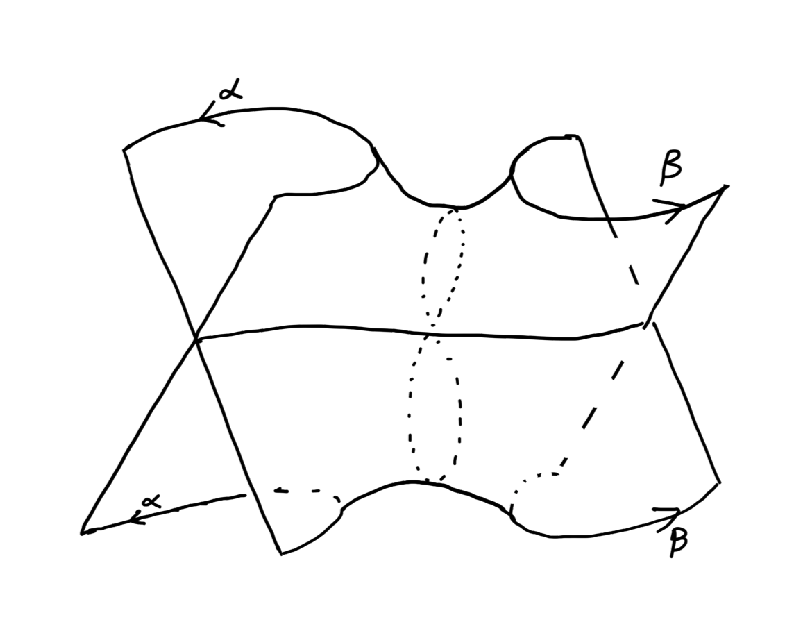
\includegraphics[scale=0.35]{images/ch4/section2/atoms/atom_foc_ell_iter1.pdf}
%\caption{Результат склейки $(\Omega, v_1)$ и $(\Omega, v_4)$.}
%\label{fig:pt9:_atom_foc_ell_iter1}
%\endminipage\hfill
%\minipage{0.43\textwidth}
%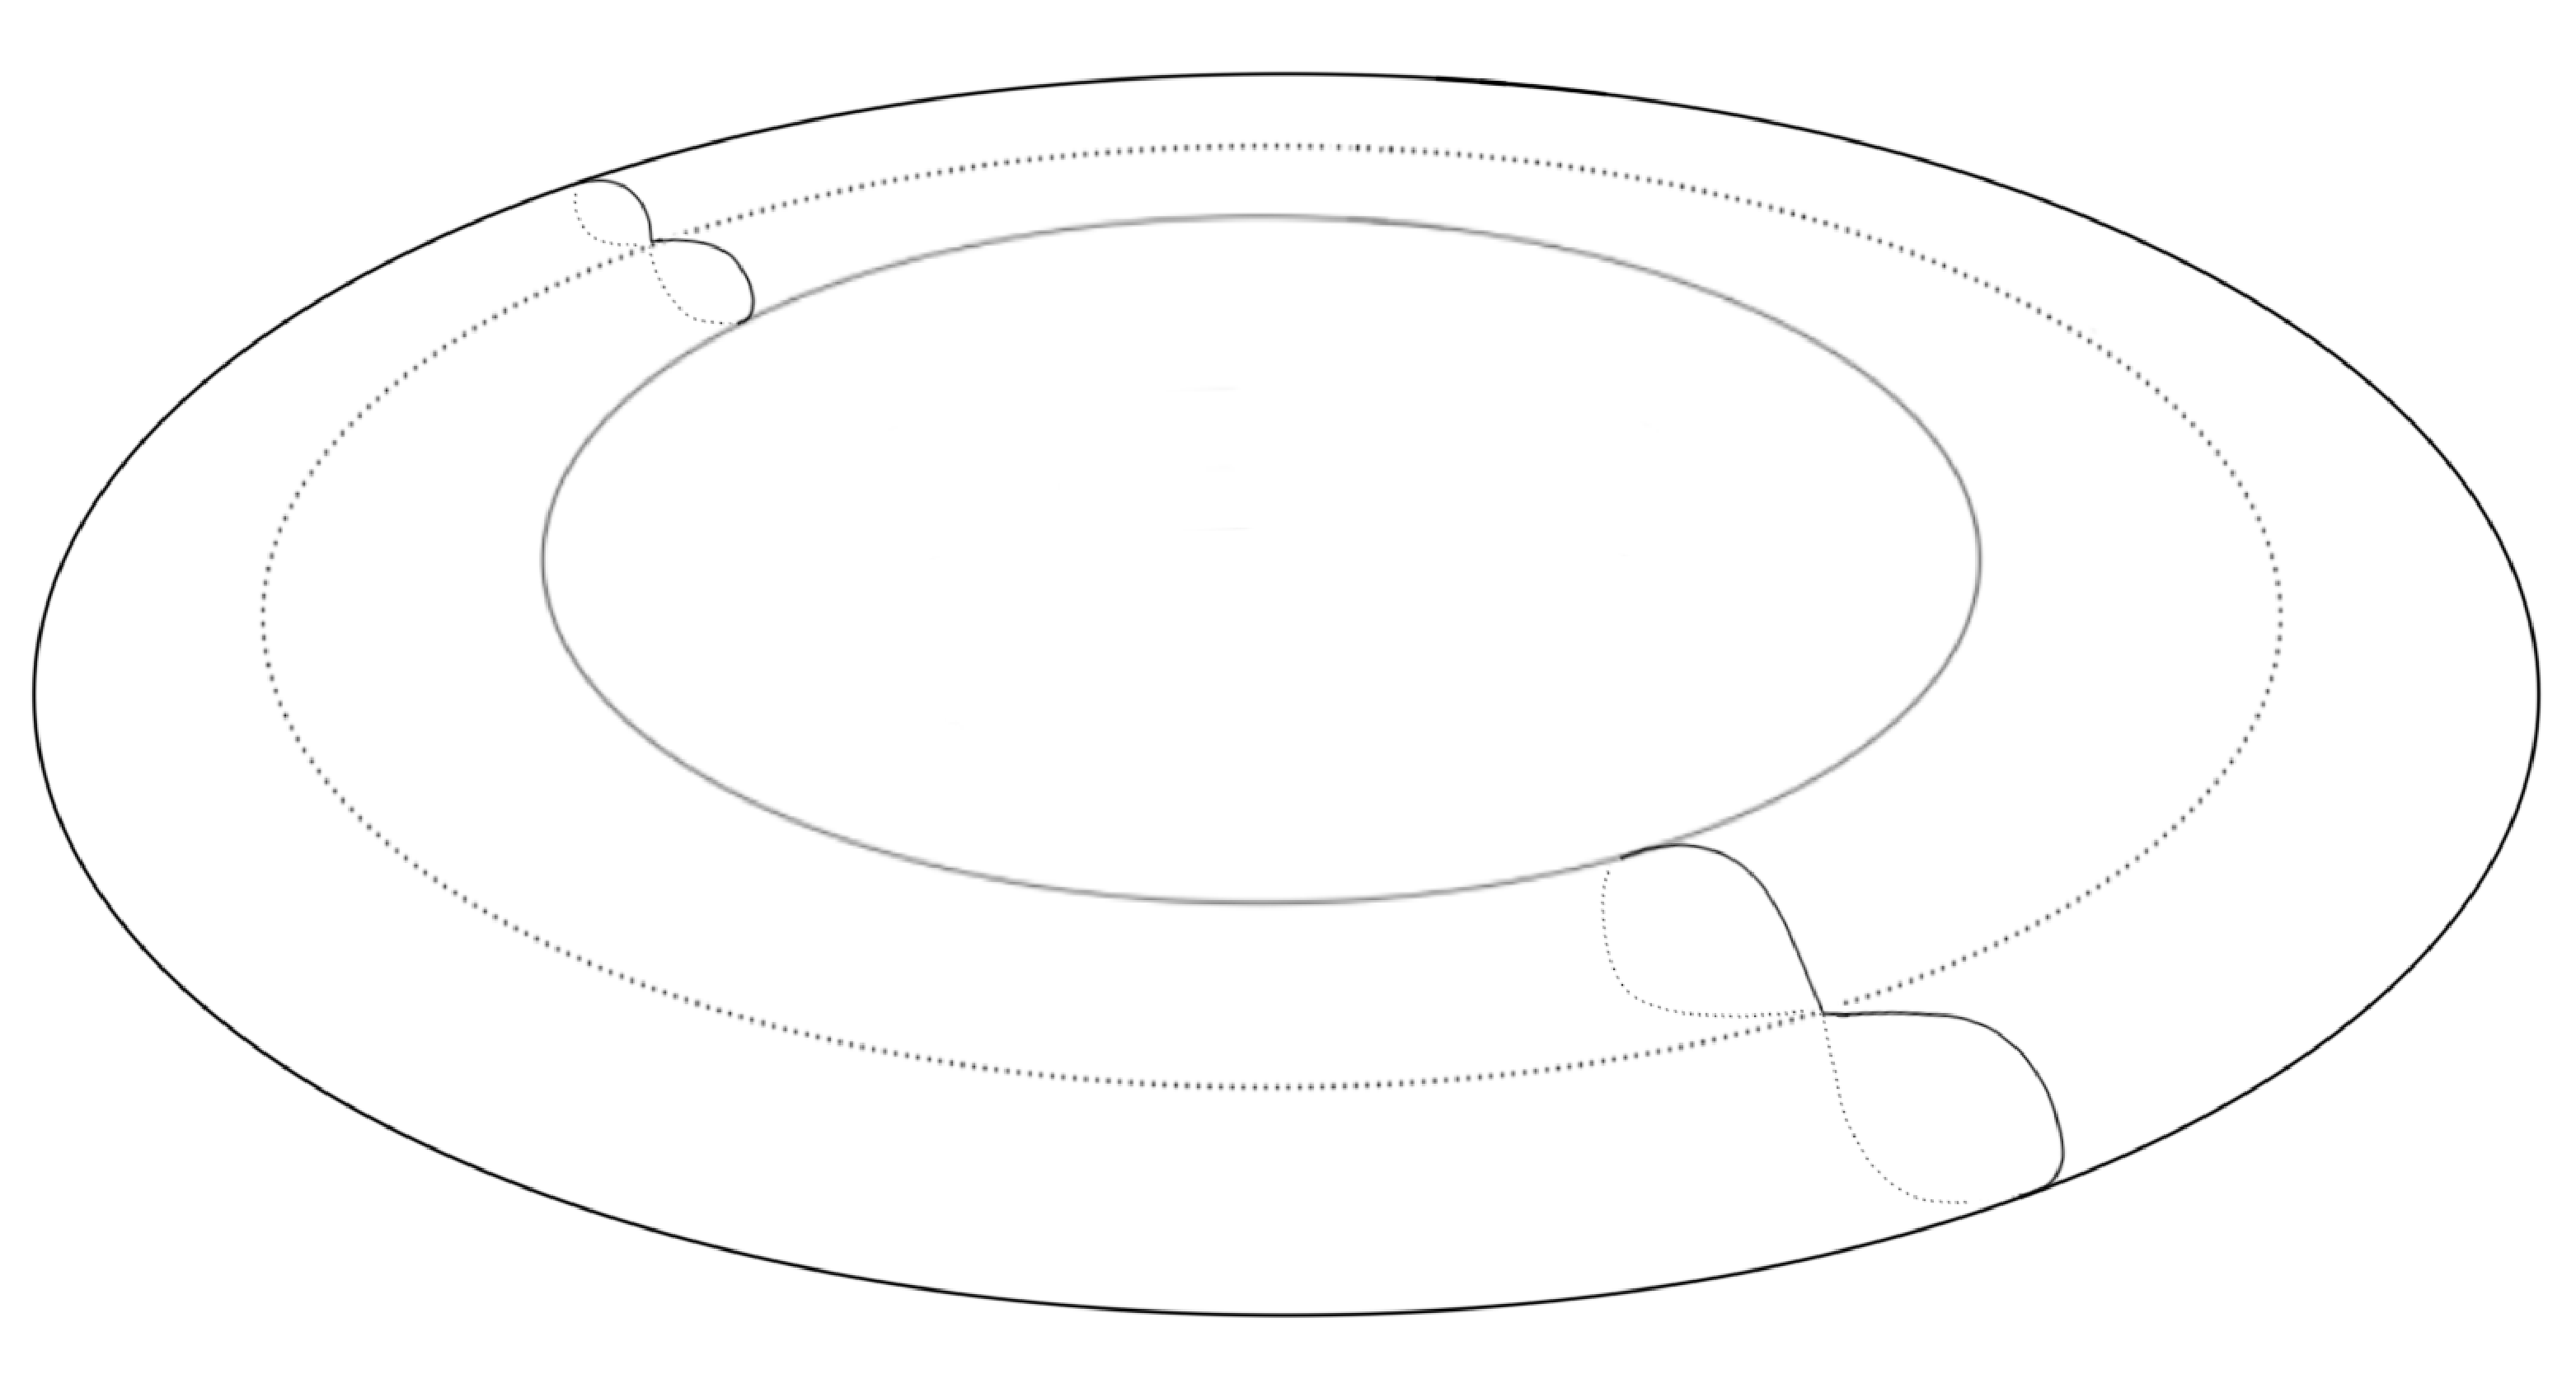
\includegraphics[scale=0.1]{images/ch4/section2/atoms/foc_ell_atom.pdf}
%\caption{Поверхность для особого значения $\Lambda=b^2 n_{in}^2$.}
%\label{fig:pt9:_foc_ell_atom}
%\endminipage\hfill
%\end{figure}

\textbf{Перестройка 3.}
Траектории бильярда в области $\Omega_{in}$ касаются эллипса с параметром $\alpha_{in}$, а в области $\Omega_{out}$ совпадают с вертикальной полуосью эллипса.

Поверхность $\Xi = \const$  можно представлять себе как предельный случай неособой поверхности $D_1^1$ (см. рис. \ref{fig:pt9:_diagramPlusIrregular}), когда две ручки <<схлопываются>> в окружности.

Более подробно, склеим листы $\widetilde{\Omega}_1$ и $\widetilde{\Omega}_4$ по общим границам, которые проецируются в эллиптические граничные дуги $\widetilde{\Omega}$ (пример области $\widetilde{\Omega}_1$ изображен на рис. \ref{fig:pt9:_hyp_page}). Аналогично для 
$\widetilde{\Omega}_2$ и $\widetilde{\Omega}_3$. Результатом склейки являются два тора с четыремя дырками каждый. При этом каждая дырка ограничена двумя дугами, которые проецируются в гиперболические граничные дуги области $\widetilde{\Omega}$. 

Области $\widetilde{\Omega}_1$ и $\widetilde{\Omega}_2$ отождествляются по дугам общей границы, которые проектируются в гиперболические граничные дуги области $\widetilde{\Omega}$, аналогично для областей $\widetilde{\Omega}_3$ и $\widetilde{\Omega}_4$. 
%В целях наглядности проденем граничные окружности друг через друга в компонентах, которые проекция $\pi$ отображает  в область $\widetilde{\Omega}_{out}$ (см. рис. \ref{fig:pt9:_atom_3_step}). Аналогично поступим с областями $\widetilde{\Omega}_2$ и $\widetilde{\Omega}_3$. 
\begin{figure}[!htb]
\minipage{0.48\textwidth}
\centering
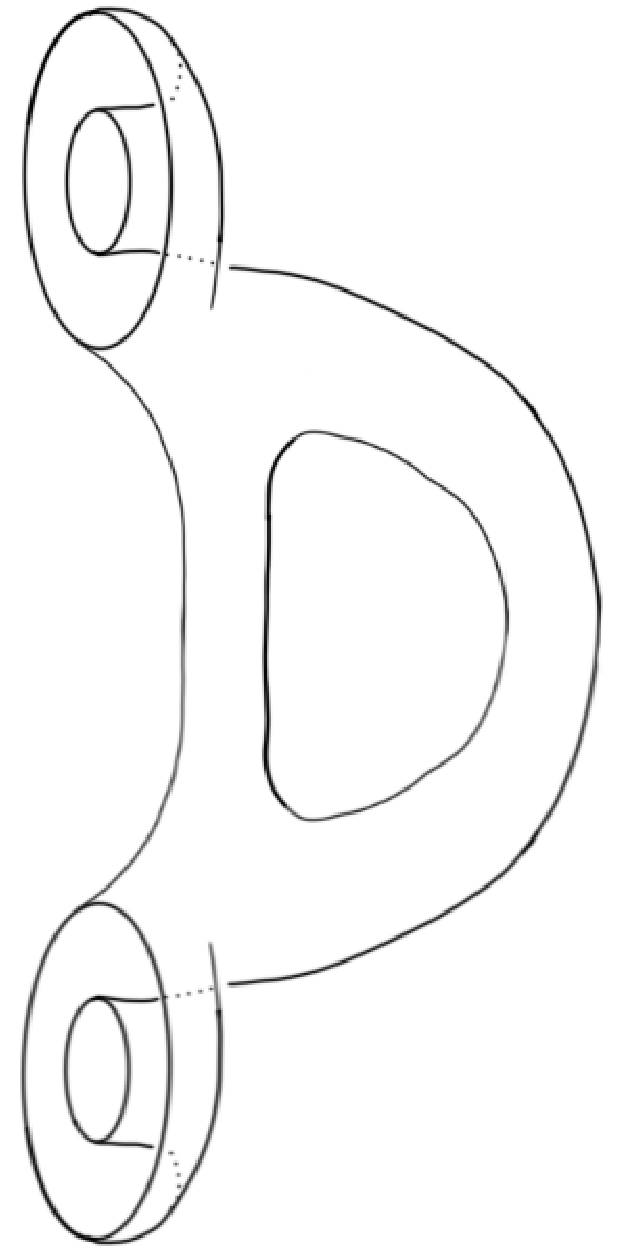
\includegraphics[scale=0.2]{images/ch4/section2/atoms/atom_3_step.pdf}
    \caption{Склейка $\widetilde{\Omega}_1 \cup \widetilde{\Omega}_4$ (перестройка 3).}
    \label{fig:pt9:_atom_3_step}
\endminipage\hfill
\minipage{0.52\textwidth}
\centering
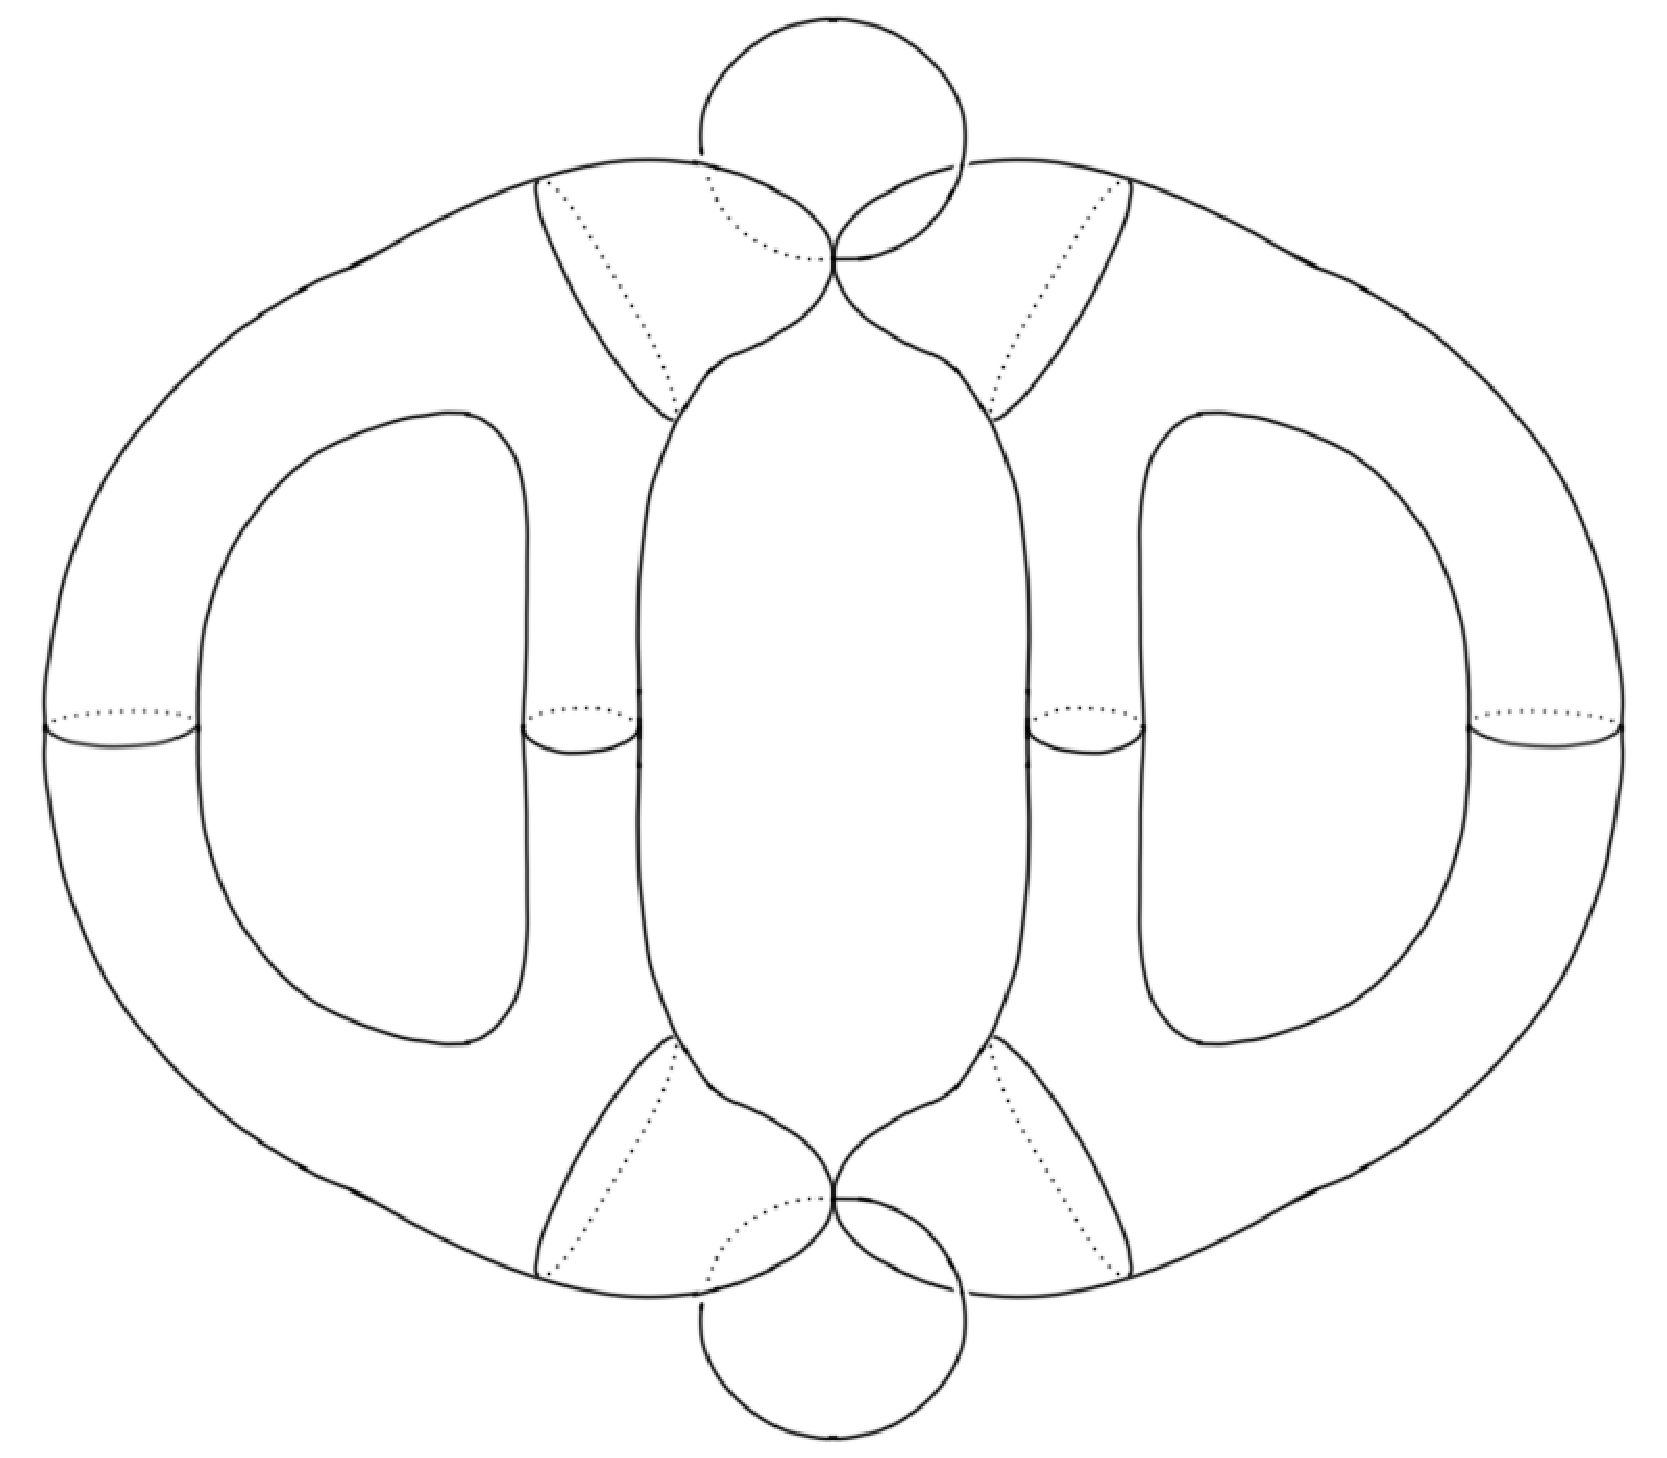
\includegraphics[scale=0.2]{images/ch4/section2/atoms/atom_3.pdf}
    \caption{Поверхность уровня $\Xi = \const$ для перестройки 3.}
    \label{fig:pt9:_atom_3}
\endminipage\hfill
\end{figure}

На рис. \ref{fig:pt9:_atom_3_step} изобразим результат склейки $\widetilde{\Omega}_1 \cup \widetilde{\Omega}_4$. Его границей являются две пары окружностей, по которым приклеивается  аналогичный результат склейки $\widetilde{\Omega}_2 \cup \widetilde{\Omega}_3$.
%К левым (внешним) окружностям $\widetilde{\Omega}_1 \cup \widetilde{\Omega}_4$ подклеим соответствующие на $\widetilde{\Omega}_2 \cup \widetilde{\Omega}_3$, а также склеим полученные поверхности по правым (внутренним). 
В момент перестройки две верхние (соответственно, две нижние) граничные окружности  $\widetilde{\Omega}_1 \cup \widetilde{\Omega}_4$ стягиваются в одну окружность. То есть поверхность $\Xi = \const$ представляет собой два касающихся в двух точках тора, при этом в каждой общей точке этих двух торов <<растет>> по одной окружности, см.  рис. \ref{fig:pt9:_atom_3}. 

\textbf{Перестройка 4.} 
Траектории бильярда в области $\Omega_{in}$ лежат на проходящих через фокусы прямых, а продолжения звеньев в области $\Omega_{out}$ касаются гиперболы с параметром $\alpha_{out}$. 

Определим область $\widetilde{\Omega}$  как объединение $\Omega_{in}$ и $\widetilde{\Omega}_{out}$, где область $\widetilde{\Omega}_{out}$ определена как пересечение $\Omega_{out}$ с областью, лежащей  между ветвями гиперболы с параметром $\alpha_{out}$. 

Горизонтальная ось пересекает область $\Omega_{in}$ по трем отрезкам, один из которых соединяет фокусы. Разрежем область $\widetilde{\Omega}$ горизонтальной осью. 
Тогда можем определить разбиение области $\widetilde{\Omega}$ на четыре области 
$\widetilde{\Omega}_{out}^u, \Omega_{in}^u, \Omega_{in}^d, \widetilde{\Omega}_{out}^d$. 
Проекция $\pi$ четырехлистна в каждой  внутренней точке любой из этих областей. Обозначим прообразы этих областей на поверхности $\Xi = \const$ как 
$\widetilde{\Omega}_{out,j}^u, \Omega_{in, j}^u, \Omega_{in, j}^d, \widetilde{\Omega}_{out, j}^d, j=1, \ldots, 4$.
Области $\Omega_{in, j}^u, \Omega_{in, j}^d, j=1,\ldots,4$ занумерованы в соответствии с правилом \eqref{eq:foc_numeration}, а области $\widetilde{\Omega}_{out,j}^u, \widetilde{\Omega}_{out, j}^d, 1, \ldots, 4$ --- как на рис. \ref{fig:pt9:_hyp_vectors_numbering}.

Области $\widetilde{\Omega}_{out,j}^u$ и $\Omega_{in, j}^u$ на поверхности $\Xi = \const$ для каждого $j=1, \ldots, 4$ отождествляются по общей границе, которая на $\widetilde{\Omega}$ проектируется в часть дуги эллипса $Q_{\lambda_1}$, заключенная между ветвями гиперболы $Q_{\alpha_{out}}$ в верхней полуплоскости. В симметричную ей дугу в нижней полуплоскости проектируется общая граница для областей $\widetilde{\Omega}_{out,1}^d$ и $\Omega_{in, 4}^d$. Аналогичным образом отождествляются дуги на границах областей $\widetilde{\Omega}_{out,2}^d$ и $\Omega_{in, 3}^d$, $\widetilde{\Omega}_{out,3}^d$ и $\Omega_{in, 2}^d$, а также $\widetilde{\Omega}_{out,4}^d$ и $\Omega_{in, 1}^d$.

В соединяющий фокусы отрезок проектируется общая граница для областей $\Omega_{in, 1}^u, \Omega_{in, 1}^d, \Omega_{in, 4}^u, \Omega_{in, 4}^d$, аналогично для областей $\Omega_{in, 2}^u, \Omega_{in, 2}^d, \Omega_{in, 3}^u, \Omega_{in, 3}^d$.
На той же прямой можно выделить отрезки, которые соединяют правый фокус с правой вершиной эллипса $Q_{\lambda_1}$. На каждый из этих отрезков проектируются границы областей $\Omega_{in, 1}^u, \Omega_{in, 2}^d, \Omega_{in, 1}^d, \Omega_{in, 2}^u$, аналогично для областей $\Omega_{in, 3}^u, \Omega_{in, 4}^d, \Omega_{in, 3}^d, \Omega_{in, 4}^u$.

Определим листы склейки $\widetilde{\Omega}_1, \ldots, \widetilde{\Omega}_4$ следующим образом (пример области $\widetilde{\Omega}_1$ см. рис. \ref{fig:pt9:_atom_4_domain}):
\begin{equation}
\begin{array}{cc}
\widetilde{\Omega}_1 = \widetilde{\Omega}_{out, 1}^u \cup \Omega_{in, 1}^u \cup \Omega_{in, 4}^d \cup \widetilde{\Omega}_{out, 1}^d, &
\widetilde{\Omega}_2 = \widetilde{\Omega}_{out, 2}^u \cup \Omega_{in, 2}^u \cup \Omega_{in, 3}^d \cup \widetilde{\Omega}_{out, 2}^d, \\
\widetilde{\Omega}_3 = \widetilde{\Omega}_{out, 3}^u \cup \Omega_{in, 3}^u \cup \Omega_{in, 2}^d \cup \widetilde{\Omega}_{out, 3}^d, &
\widetilde{\Omega}_4 = \widetilde{\Omega}_{out, 4}^u \cup \Omega_{in, 4}^u \cup \Omega_{in, 1}^d \cup \widetilde{\Omega}_{out, 4}^d.
\end{array}
\label{eq:case4Omegas}
\end{equation}
\begin{figure}[!htb]
\centering
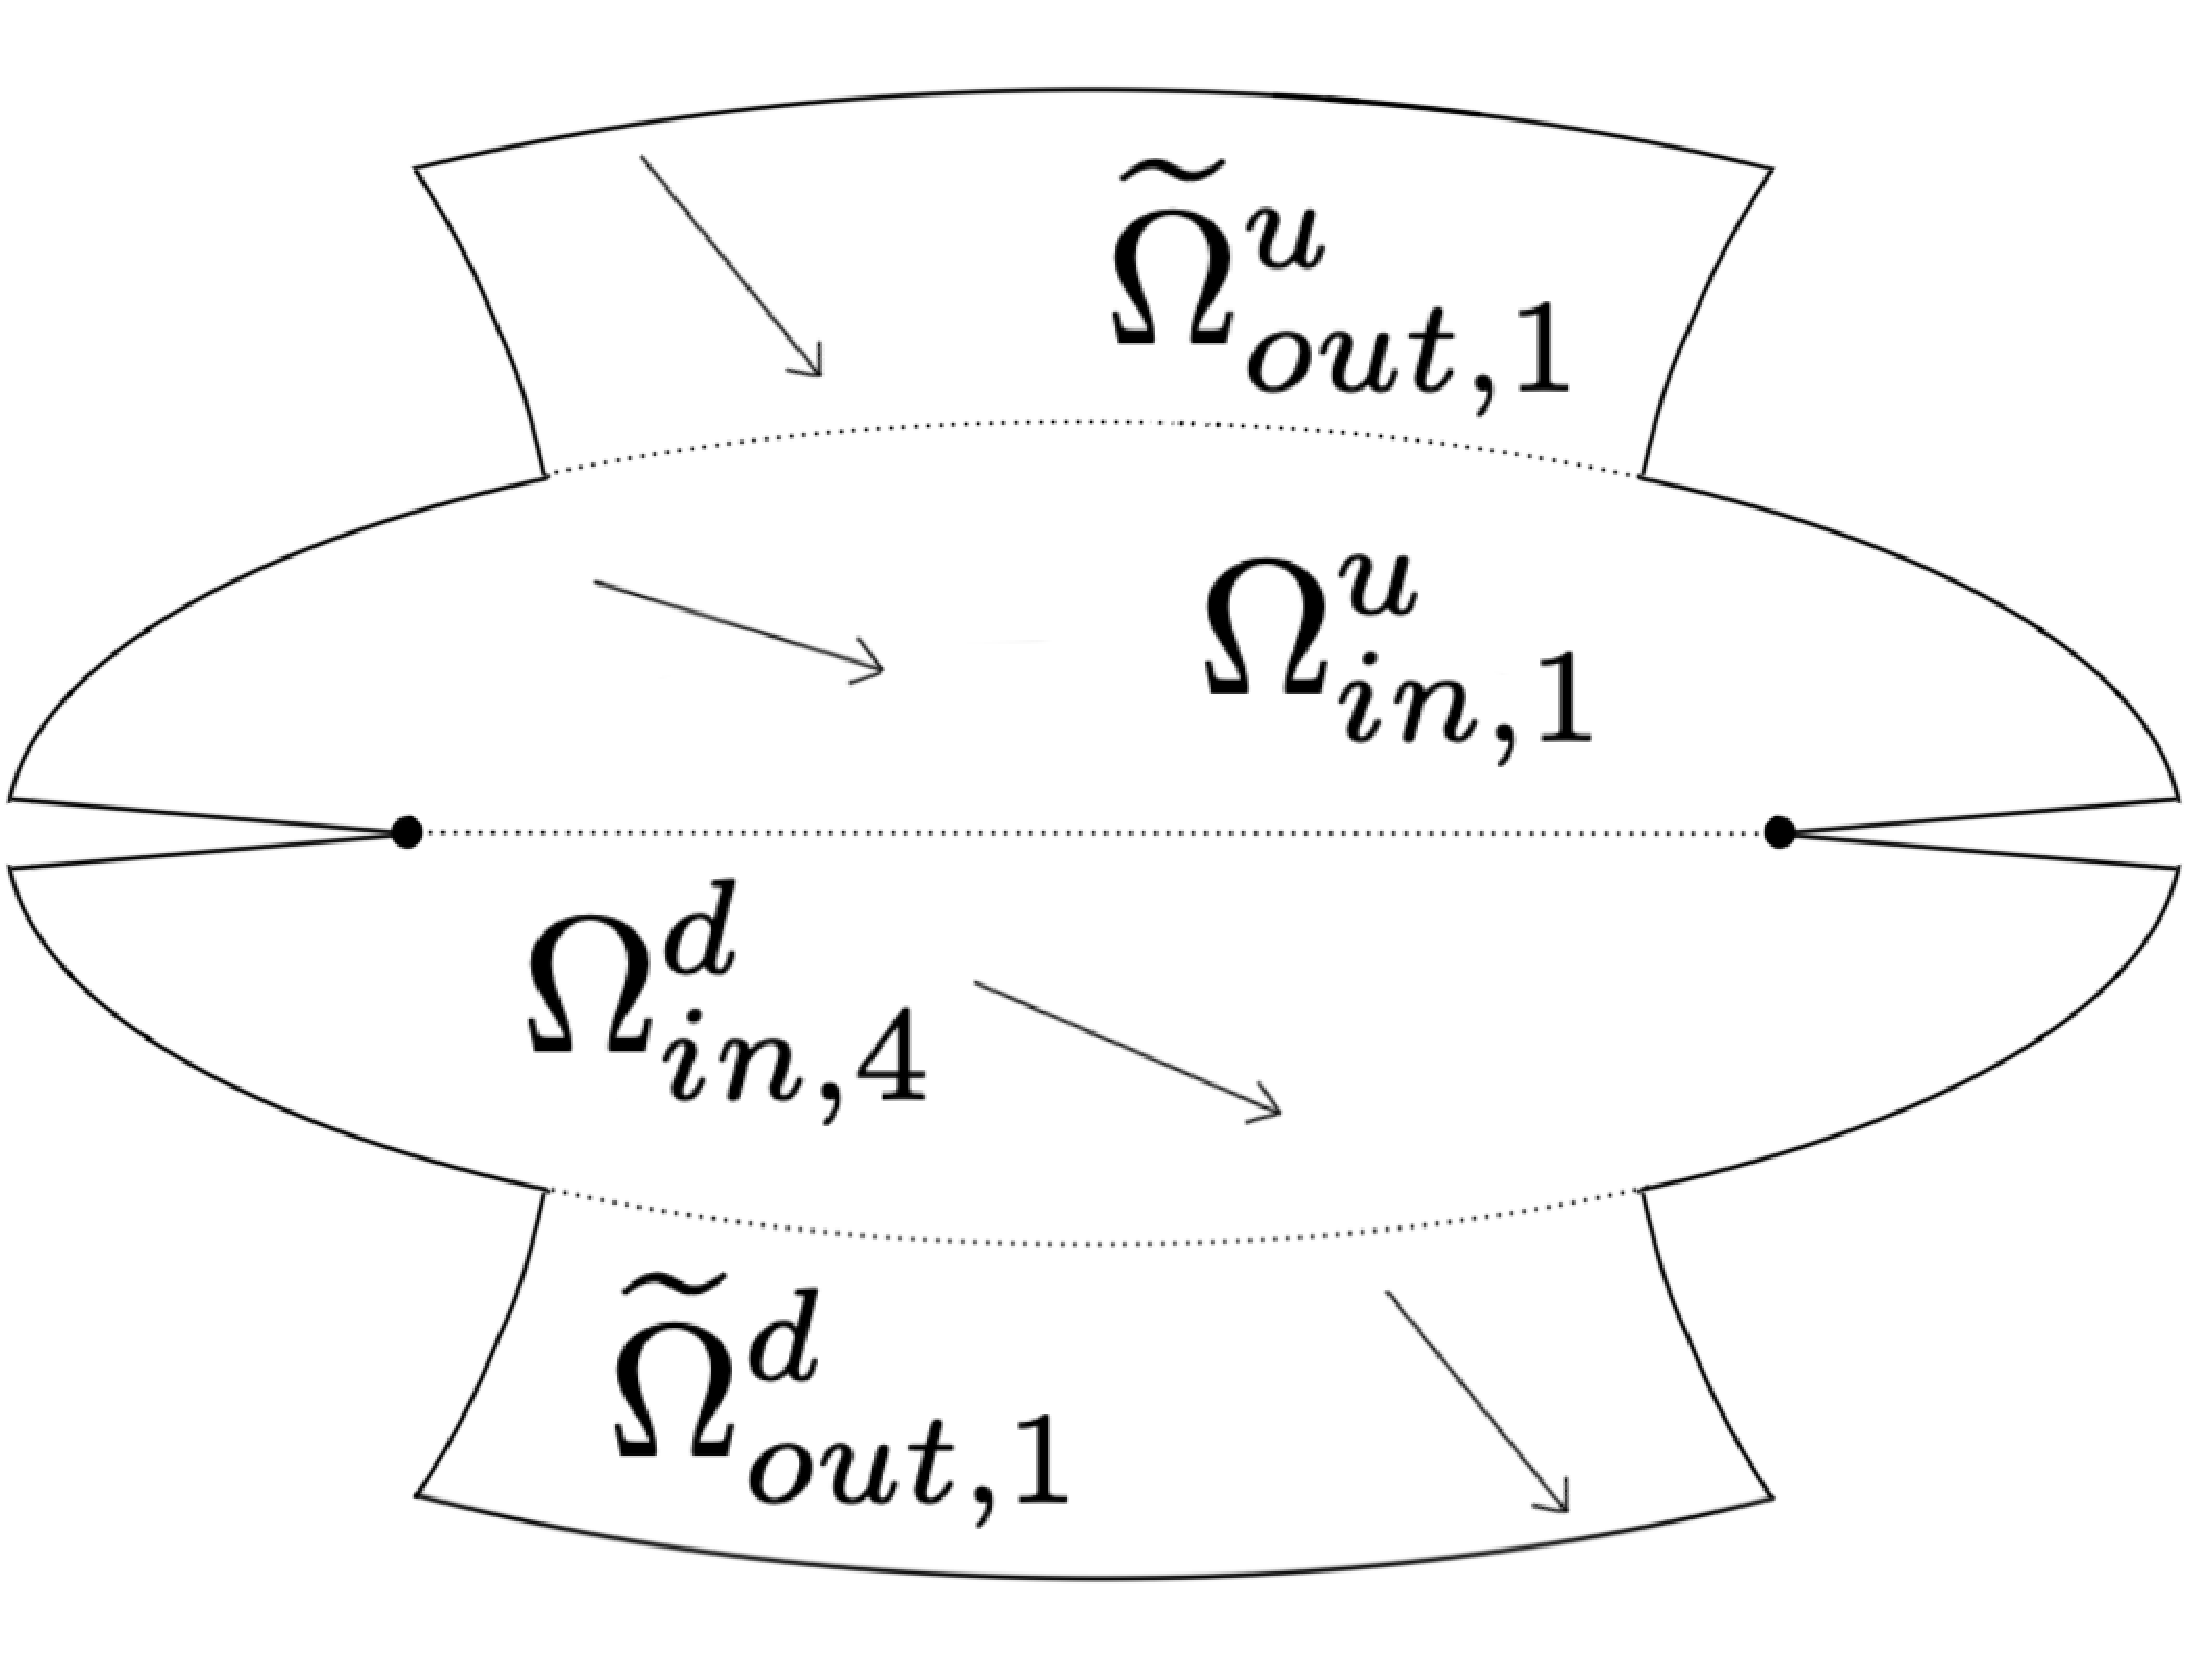
\includegraphics[width=5cm]{images/ch4/section2/atoms/atom_4_domain.pdf}
    \caption{Пример области $\widetilde{\Omega}_1$ для перестройки 4.}
    \label{fig:pt9:_atom_4_domain}
\end{figure}


Склеим листы $\widetilde{\Omega}_1$ и  $\widetilde{\Omega}_4$ по общим граничным дугам на поверхности $\Xi = \const$, которые проецируются на эллиптические граничные дуги области $\widetilde{\Omega}$, а также на  
%проецирующимся в эллиптические . Точнее, по двум дугам, проектирующимся на граничный эллипс между ветвей гиперболы $Q_{\alpha_{out}}$, а также по дугам, проектирующимися на  эллипс $Q_{\lambda_1}$ вне указанных ветвей. 
%Листы $\widetilde{\Omega}_1$ и  $\widetilde{\Omega}_4$ также склеим по граничной дуге на поверхности, которая проектируется на 
соединяющий фокусы отрезок. Аналогичные склейки повторим для листов $\widetilde{\Omega}_2$ и  $\widetilde{\Omega}_3$. Результатом склеек являются две фигуры, каждая из которых является склейкой цилиндров с двумя дырками вдоль общей горизонтальной направляющей (см. рис. \ref{fig:pt9:_atom_foc_hyp_iter1}).


Ветви гиперболы с параметром $\alpha_{out}$ пересекаются с областью $\widetilde{\Omega}_{out}$ по четырем дугам, в каждую из которых проектируются по две дуги на $\Xi = \const$, ограничивающие одну из дырок на склейке $\widetilde{\Omega}_1 \cup \widetilde{\Omega}_4$. Аналогично для склейки $\widetilde{\Omega}_2 \cup \widetilde{\Omega}_3$. При этом на дуги в верхней полуплоскости проектируются общие границы для $\widetilde{\Omega}_{out, 1}^u$ и $\widetilde{\Omega}_{out, 4}^u$, а также $\widetilde{\Omega}_{out, 2}^u$ и $\widetilde{\Omega}_{out, 3}^u$. Аналогичные склейки для $\widetilde{\Omega}_{out, 1}^d$ и $\widetilde{\Omega}_{out, 4}^d$, а также $\widetilde{\Omega}_{out, 2}^d$ и $\widetilde{\Omega}_{out, 3}^d$ возникают на прообразе дуг в нижней полуплоскости.

Граничные окружности цилиндров проецируются на отрезки $\{y=0\} \cap \Omega_{in}$ вне фокусов. Точнее, в правый такой отрезок проектируются пары дуг $\Omega_{in, 1}^u \cap \Omega_{in, 4}^u$, $\Omega_{in, 1}^d \cap \Omega_{in, 4}^d$, которые ограничивают верхнюю и нижнюю граничные окружности, соответственно. Аналогично для пар дуг $\Omega_{in, 2}^u \cap \Omega_{in, 3}^u$, $\Omega_{in, 2}^d \cap \Omega_{in, 3}^d$. 
По этим граничным окружностям склеим также возникают склейки $\widetilde{\Omega}_1 \cup \widetilde{\Omega}_4$ и $\widetilde{\Omega}_2 \cup \widetilde{\Omega}_3$. 
Торцевые окружности при этом в правой части подклеиваются с <<перекруткой>>: \textit{нижняя} граничная окружность $\widetilde{\Omega}_1 \cup \widetilde{\Omega}_4$ отождествляется с \textit{верхней} окружностью на $\widetilde{\Omega}_2 \cup \widetilde{\Omega}_3$, аналогично \textit{верхняя} на $\widetilde{\Omega}_1 \cup \widetilde{\Omega}_4$ --- с \textit{нижней} на $\widetilde{\Omega}_2 \cup \widetilde{\Omega}_3$.
Аналогичные соображения для тех же листов справедливы в симметричном отрезке в левой полуплоскости.

Остается склеить отождествить $\widetilde{\Omega}_1 \cup \widetilde{\Omega}_4$ и $\widetilde{\Omega}_2 \cup \widetilde{\Omega}_3$ по указанным дугам (см. рис. \ref{fig:pt9:_atom_foc_hyp_iter1}).
%
%
%Соответствует случаю $\alpha_{in} = b^2, \ \alpha_{out} \in (b^2, a^2)$. 
%Область приведена на Рис. \ref{fig:pt9:_atom_4_domain}. В области $\Omega_{out}$ траектории касаются гиперболы, а во внутренней области $\Omega_{in}$ --- направлены к одному из фокусов. 
%Повторяя изложенные выше соображения, разрежем ту часть области $\Omega$, в которой траектории направлены к одному из фокусов, по отрезкам от фокуса до внешней эллиптической границы. 
%При этом на соединяющем фокусы отрезке появится склейка первого и четвертого листов. Результат после этой склейки изображен на Рис. \ref{fig:pt9:_atom_foc_hyp_iter1}
Результирующая поверхность $\Xi = \const$ изображена на рис. \ref{fig:pt9:_atom_4}.

\begin{figure}[!htb]
\minipage{0.5\textwidth}
\centering
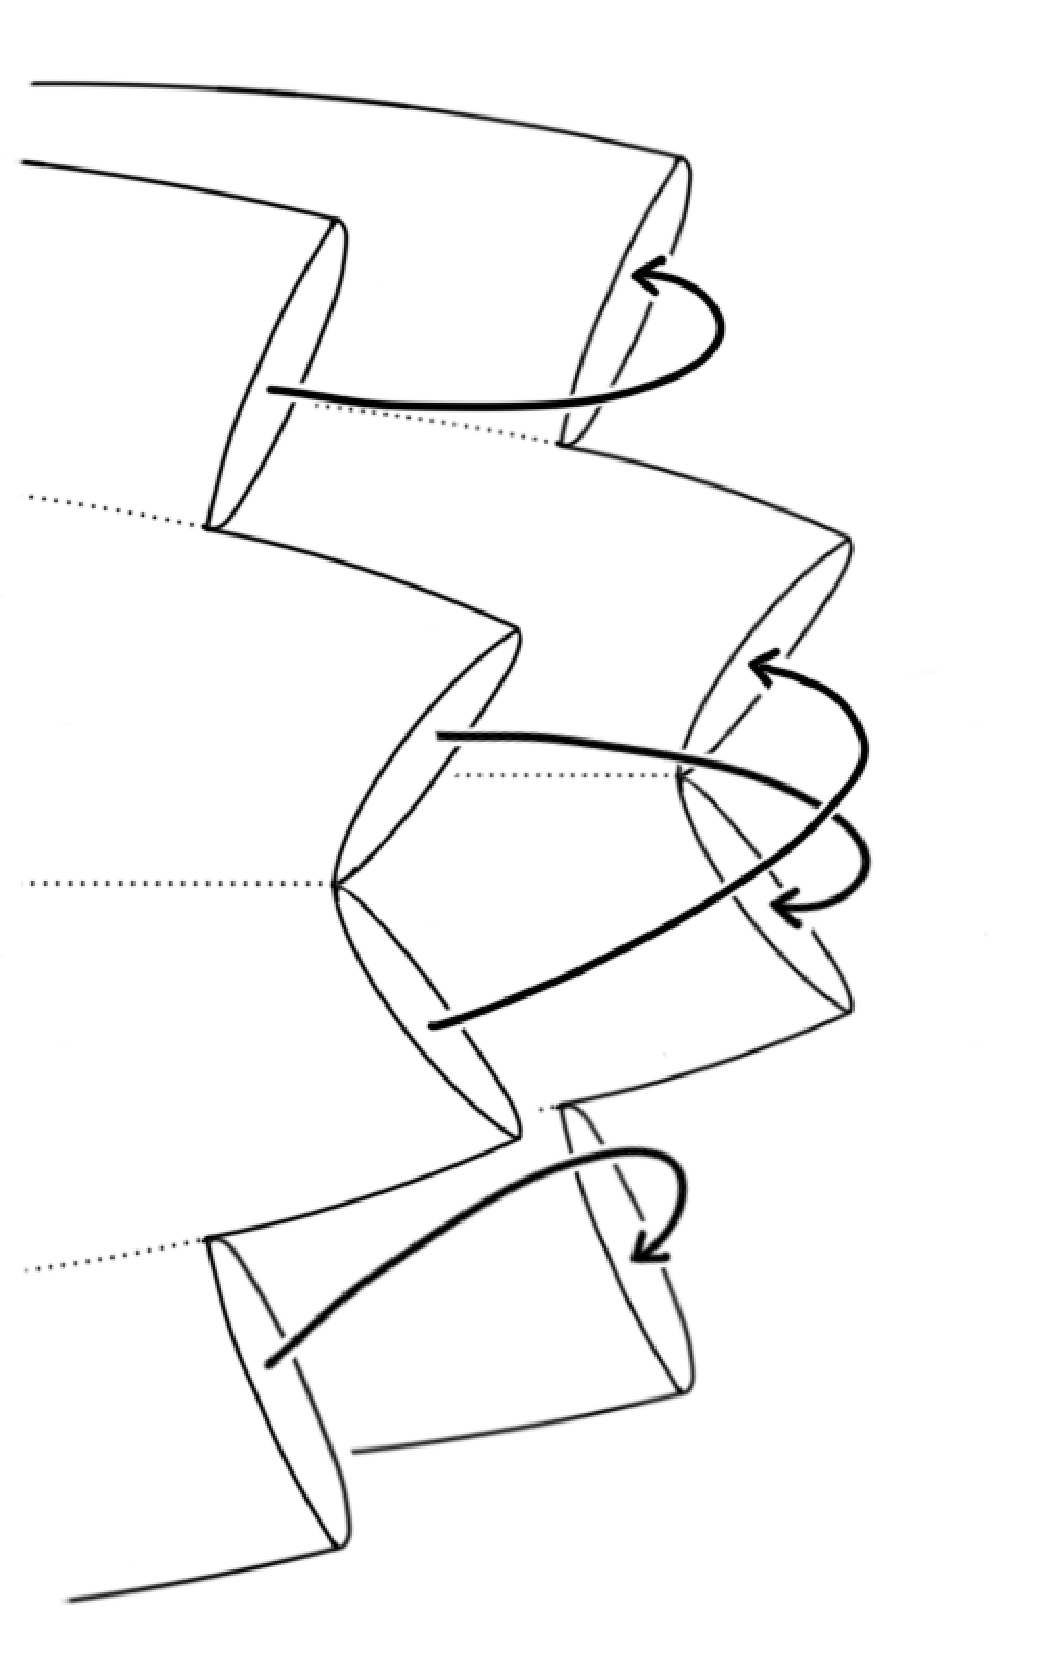
\includegraphics[width=3cm]{images/ch4/section2/atoms/atom_foc_hyp_iter1.pdf}
    \caption{Схема склейки $\widetilde{\Omega}_1 \cup \widetilde{\Omega}_4$ (на переднем плане) и $\widetilde{\Omega}_2 \cup \widetilde{\Omega}_3$ (на заднем плане).}
    \label{fig:pt9:_atom_foc_hyp_iter1}
    \endminipage\hfill
\minipage{0.5\textwidth}
    \centering
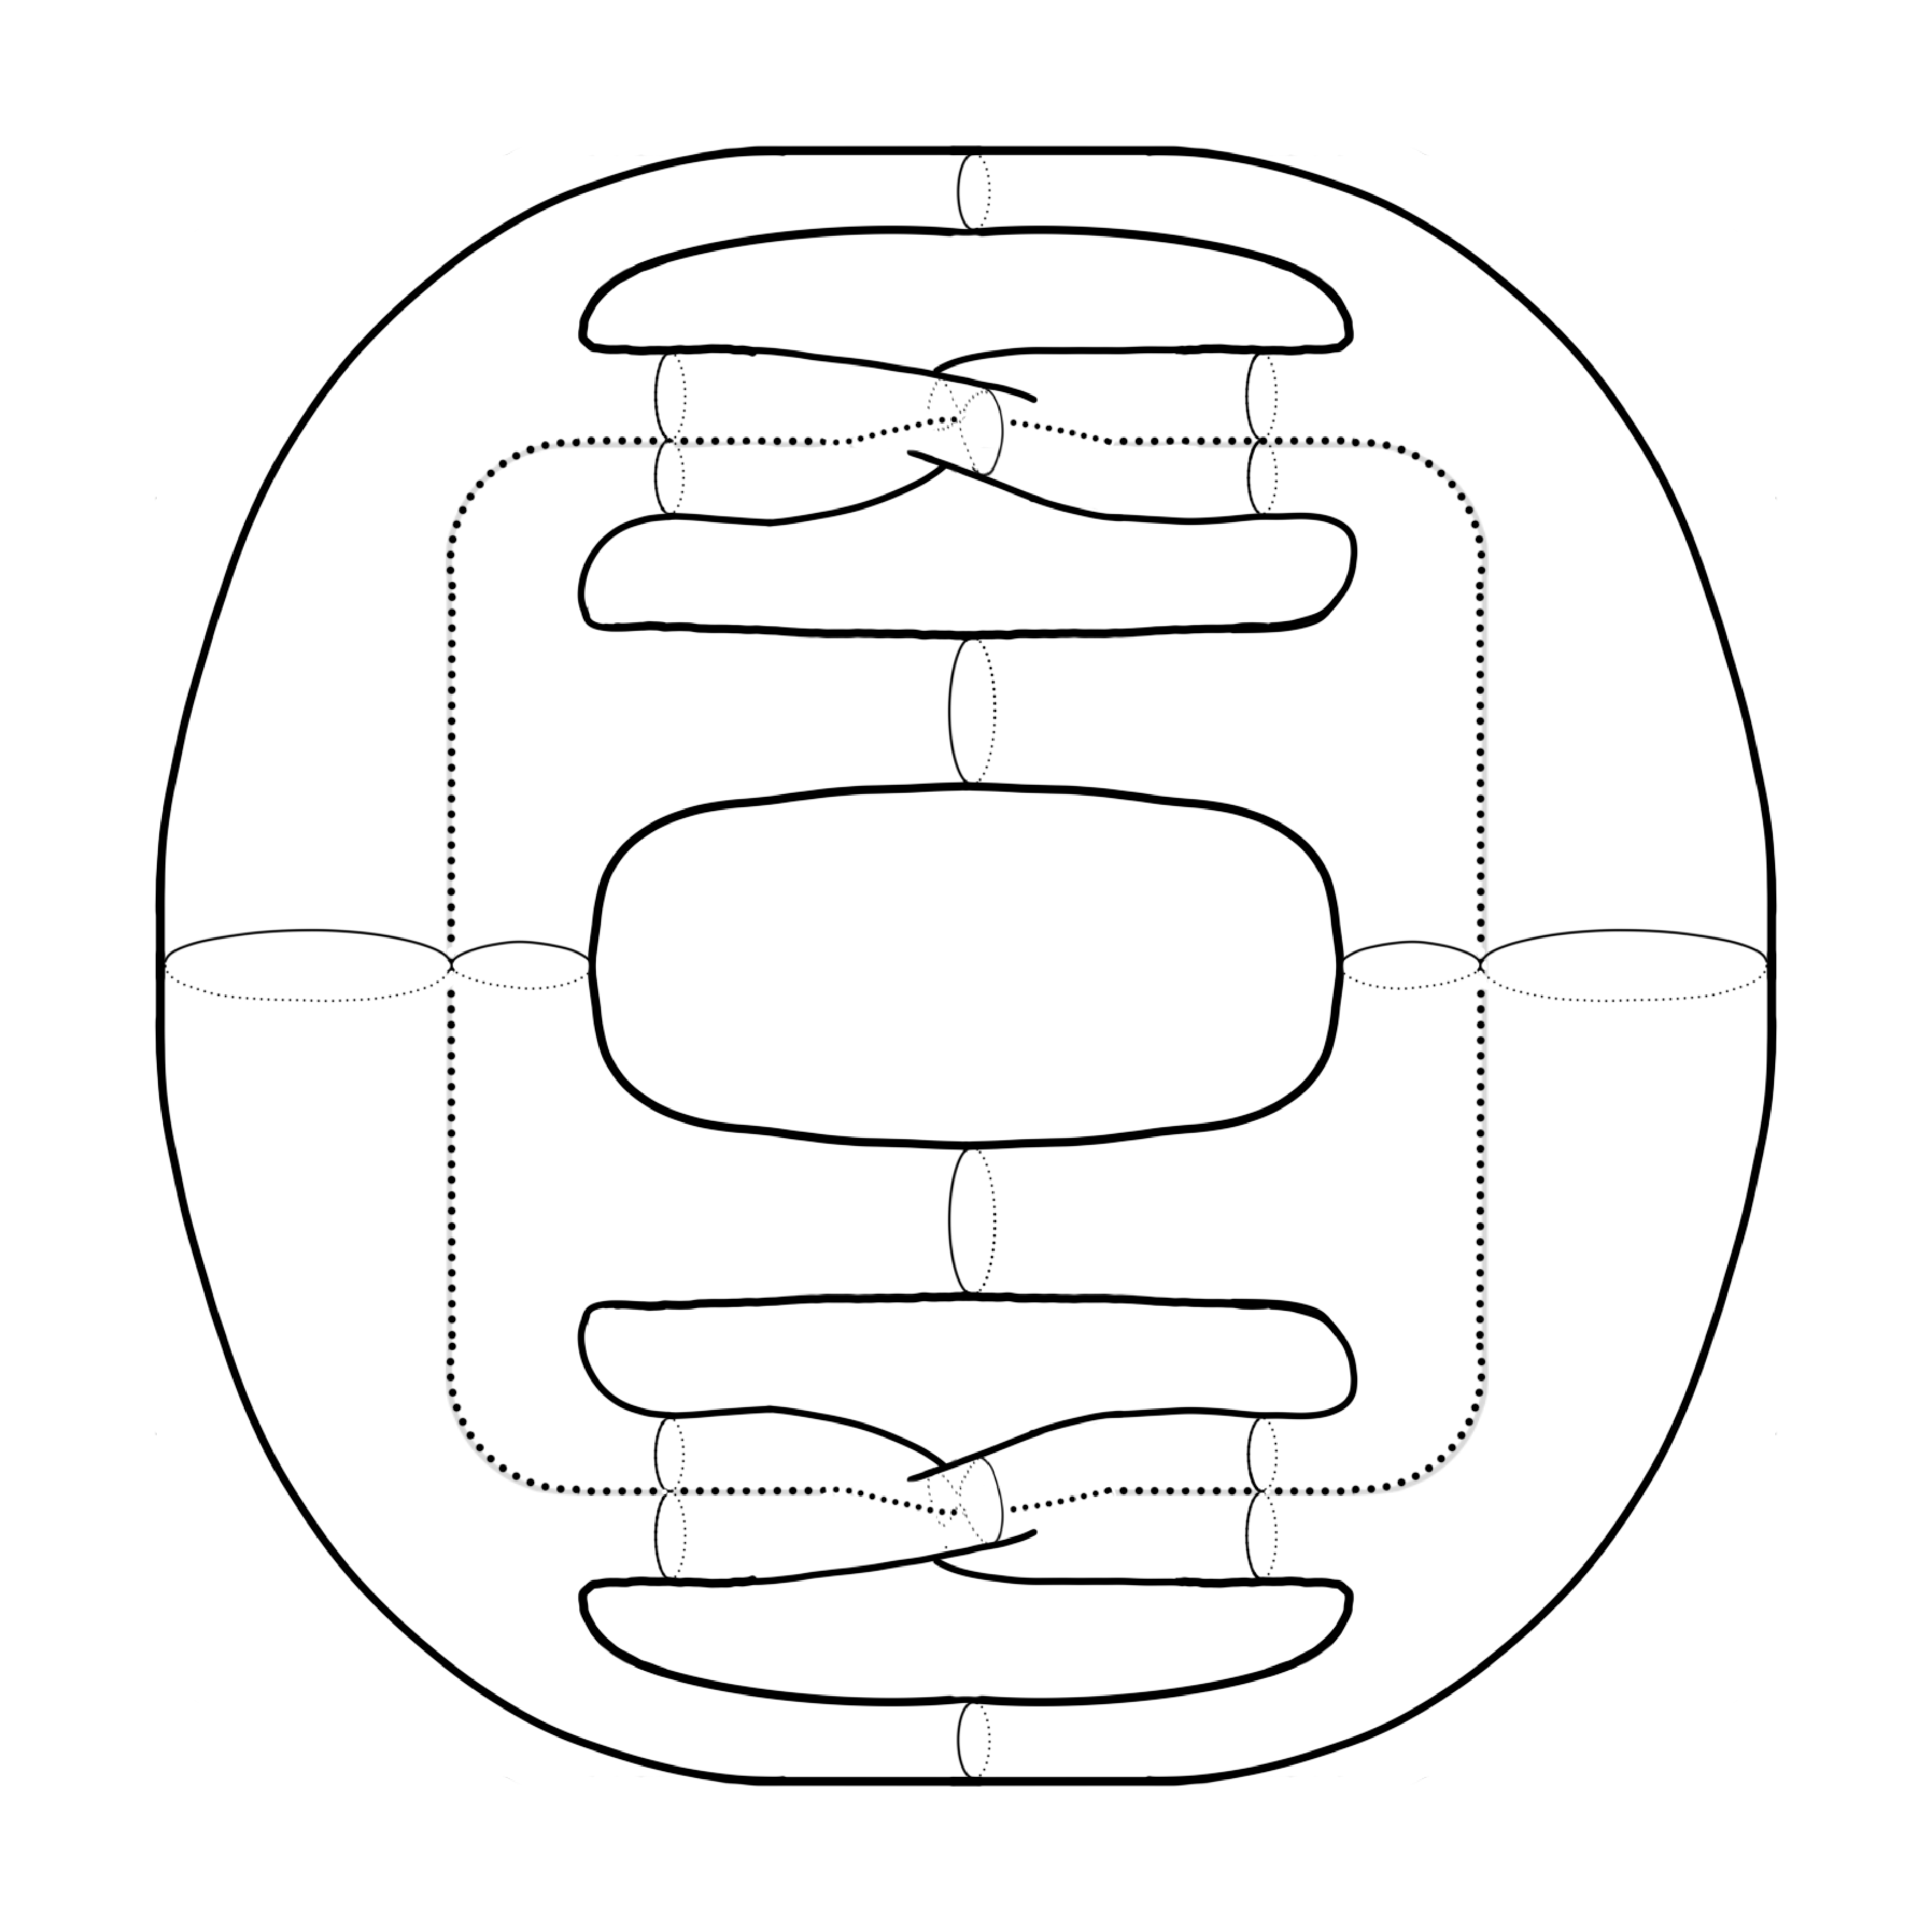
\includegraphics[width=5cm]{images/ch4/section2/atoms/atom_4.pdf}
    \caption{Поверхность уровня $\Xi = \const$ для перестройки 4.}
    \label{fig:pt9:_atom_4}
\endminipage\hfill
\end{figure}

\textbf{Перестройка 5.} 
Звенья траектории в области $\Omega_{in}$ касаются гиперболы с параметром $\alpha_{in}$, а в области $\Omega_{out}$ лежат на проходящих через фокусы прямых.

Определим область $\widetilde{\Omega}_{in}$ как часть эллипса $\Omega_{in}$ между ветвей гиперболы с параметром $\alpha_{in}$. 
Область $\widetilde{\Omega}$ определим как объединение $\widetilde{\Omega}_{in} \cup \Omega_{out}$.

Проекция поверхности $\Xi = \const$ на область $\widetilde{\Omega}$ четырехлистна в каждой внутренней точке $\widetilde{\Omega}$ кроме отрезков $\Omega_{out} \cap \{y=0\}$.
Разрежем $\Omega_{out}$ вдоль этих горизонтальных отрезков и получим области $\Omega_{out}^u,  \Omega_{out}^d$. 
Тогда проекция четырехлистна в каждой области $\widetilde{\Omega}_{in}, \Omega_{out}^u,  \Omega_{out}^d$. Прообразы этих областей на поверхности $\Xi = \const$  обозначим как $\widetilde{\Omega}_{in, j}, \Omega_{out, j}^u,  \Omega_{out, j}^d, j=1,\ldots, 4$. 
При этом области $\Omega_{out, j}^u,  \Omega_{out, j}^d$ занумерованы  в соответствии с правилом \eqref{eq:foc_numeration}, а области $\widetilde{\Omega}_{in, j}$ --- как на рис. \ref{fig:pt9:_hyp_vectors_numbering}.

На поверхности $\Xi = \const$ области $\widetilde{\Omega}_{in, j}$ и $\Omega_{out, j}^u$ для каждого $j=1, \ldots,4$  отождествляются по дуге, которая проектируется в $\widetilde{\Omega}$ на дугу эллипса $Q_{\lambda_1}$, заключенную между ветвями гиперболы с параметром $\alpha_{in}$ в верхней полуплоскости. На симметричную дугу в нижней полуплоскости проектируются общие граничные дуги для областей $\widetilde{\Omega}_{in, 1}$ и $\Omega_{out, 4}^d$, аналогично для пары областей $\widetilde{\Omega}_{in, 2}$ и $\Omega_{out, 3}^d$, для пары $\widetilde{\Omega}_{in, 3}$ и $\Omega_{out, 2}^d$, а также для пары $\widetilde{\Omega}_{in, 4}$ и $\Omega_{out, 1}^d$. 

Определим листы $\widetilde{\Omega}_1, \ldots, \widetilde{\Omega}_4$. 
\begin{equation}
\begin{array}{cc}
\widetilde{\Omega}_1 = \Omega_{out, 1}^u \cup \widetilde{\Omega}_{in, 1} \cup \Omega_{out, 4}^d, &
\widetilde{\Omega}_2 = \Omega_{out, 2}^u \cup \widetilde{\Omega}_{in, 2} \cup \Omega_{out, 3}^d, \\
\widetilde{\Omega}_3 = \Omega_{out, 3}^u \cup \widetilde{\Omega}_{in, 3} \cup \Omega_{out, 2}^d, &
\widetilde{\Omega}_4 = \Omega_{out, 4}^u \cup \widetilde{\Omega}_{in, 4} \cup \Omega_{out, 1}^d.
\end{array}
\label{eq:case5Omegas}
\end{equation}
Пример области $\widetilde{\Omega}_1$ изображен на рис. \ref{fig:pt9:_domain_atom_hyp_foc}.

\begin{figure}[!htb]
\minipage{0.5\textwidth}
\centering
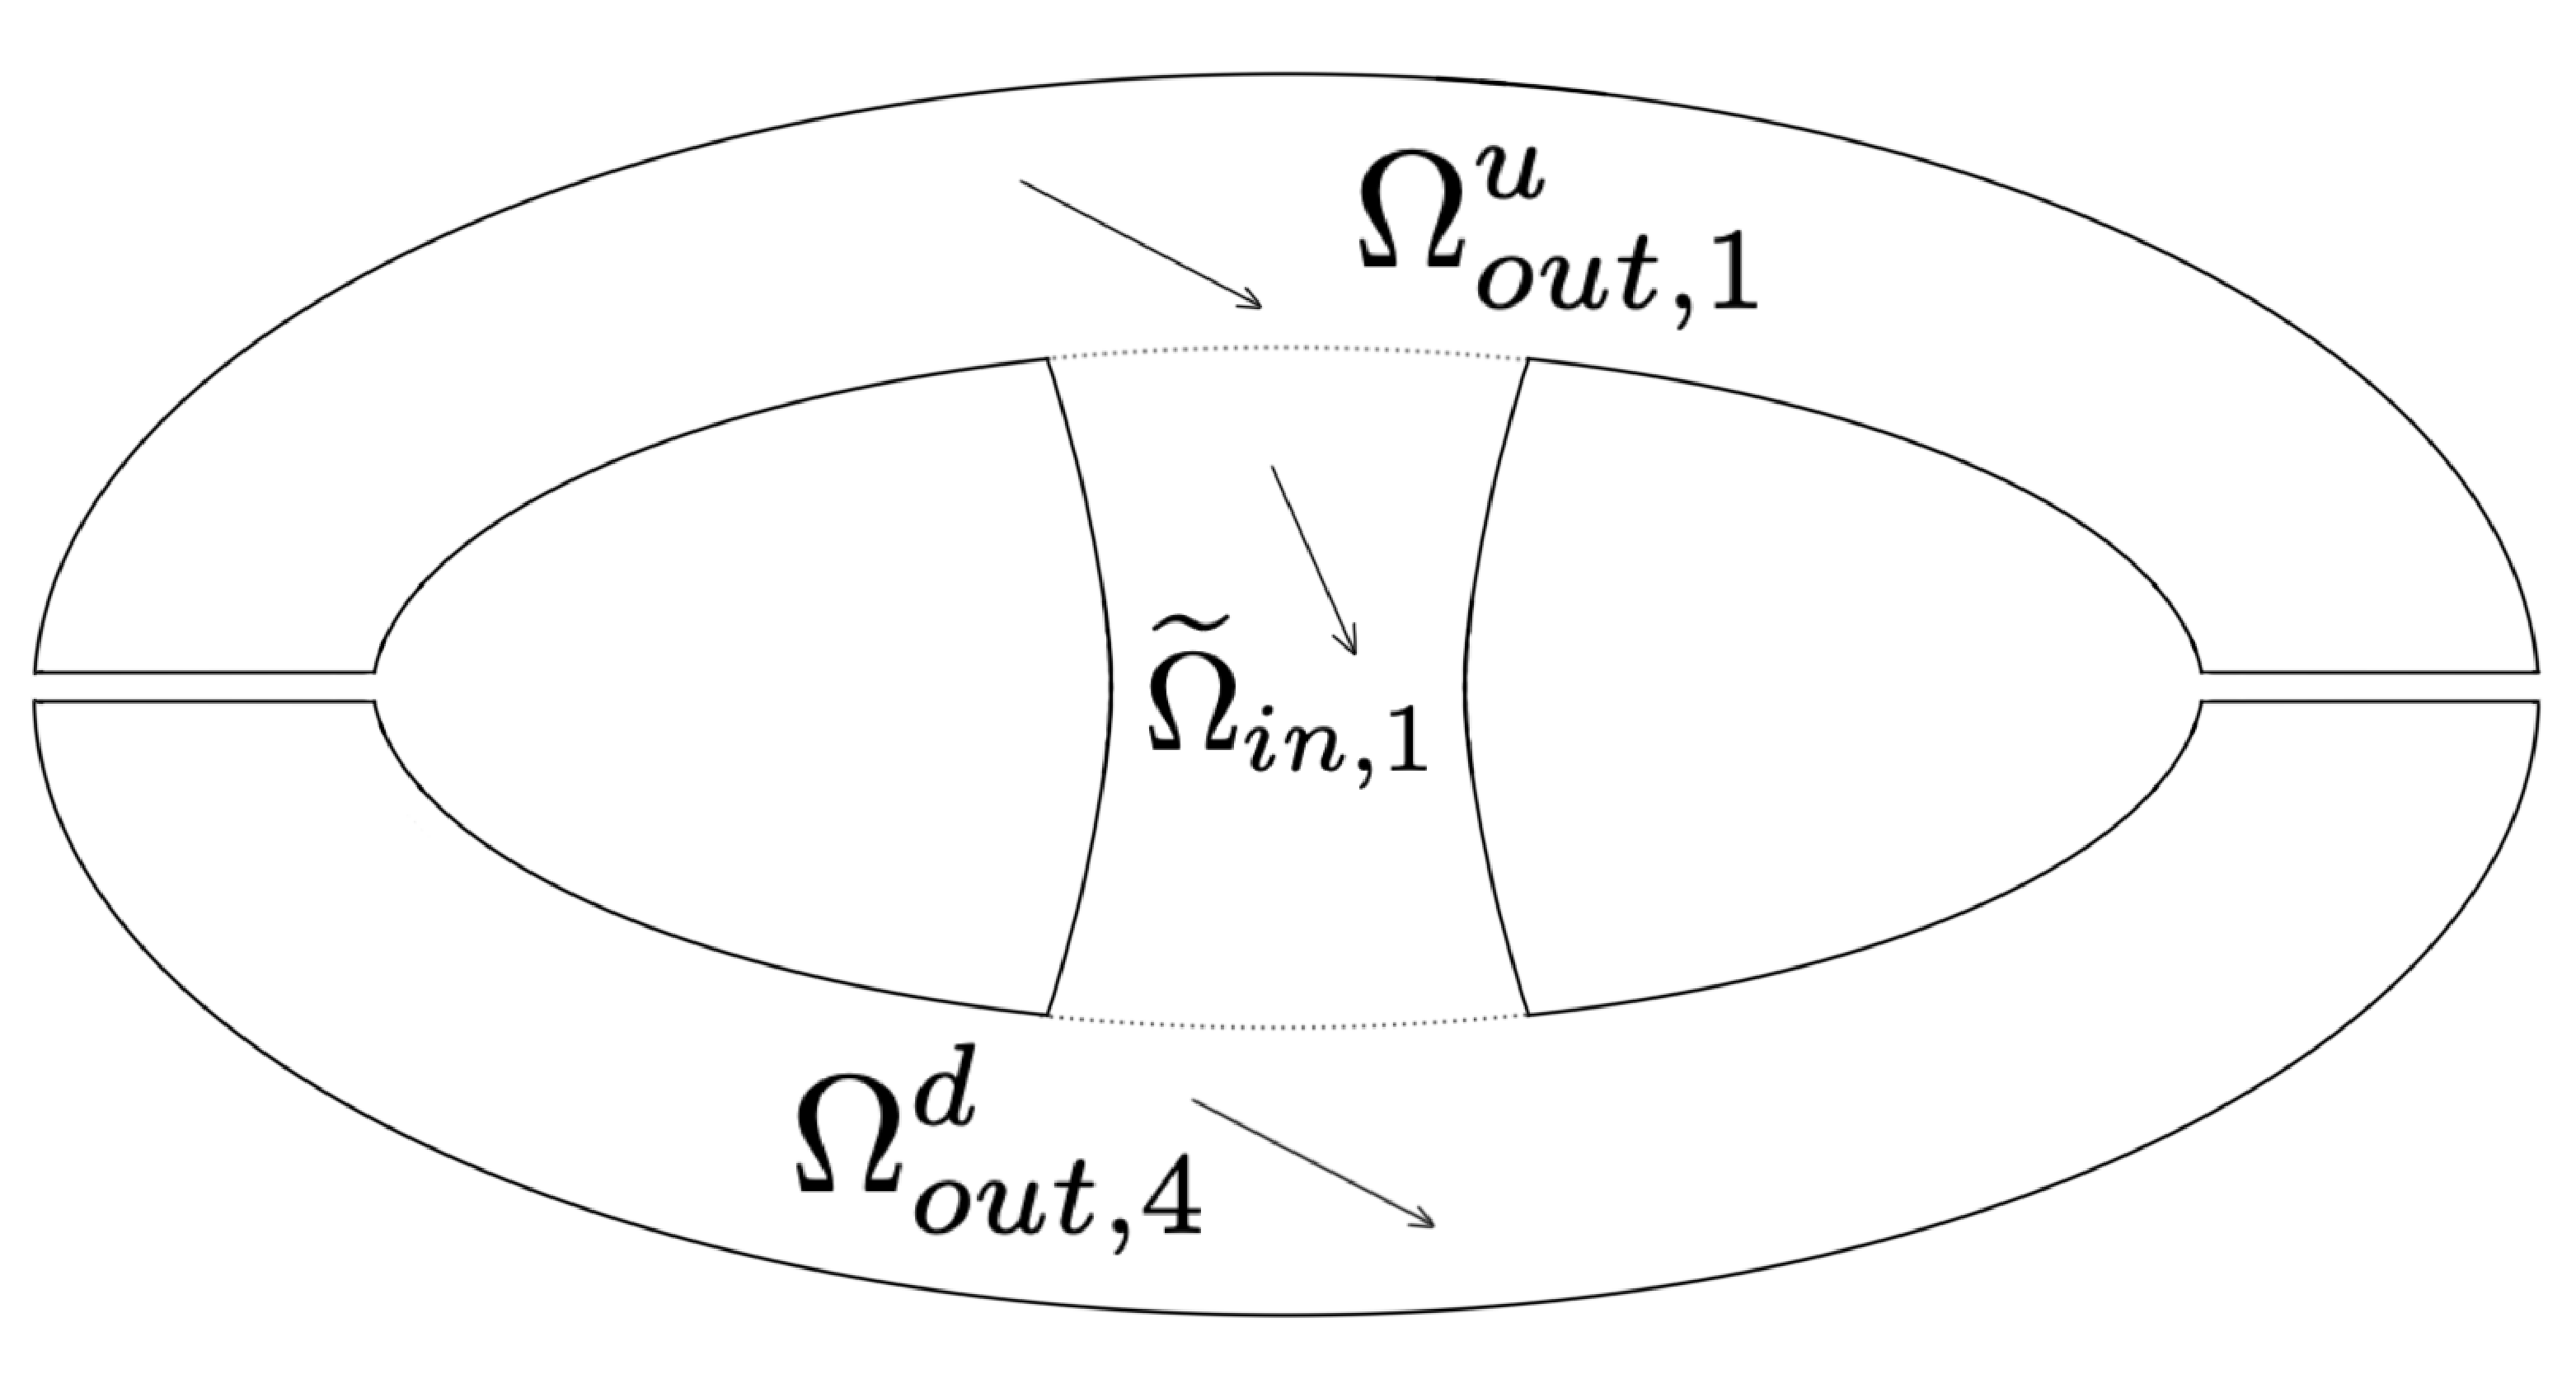
\includegraphics[scale=0.1]{images/ch4/section2/atoms/atom_5_domain.pdf}
    \caption{Пример области $\widetilde{\Omega}_1$ для перестройки 5.}
    \label{fig:pt9:_domain_atom_hyp_foc}
\endminipage\hfill
\minipage{0.5\textwidth}
\centering
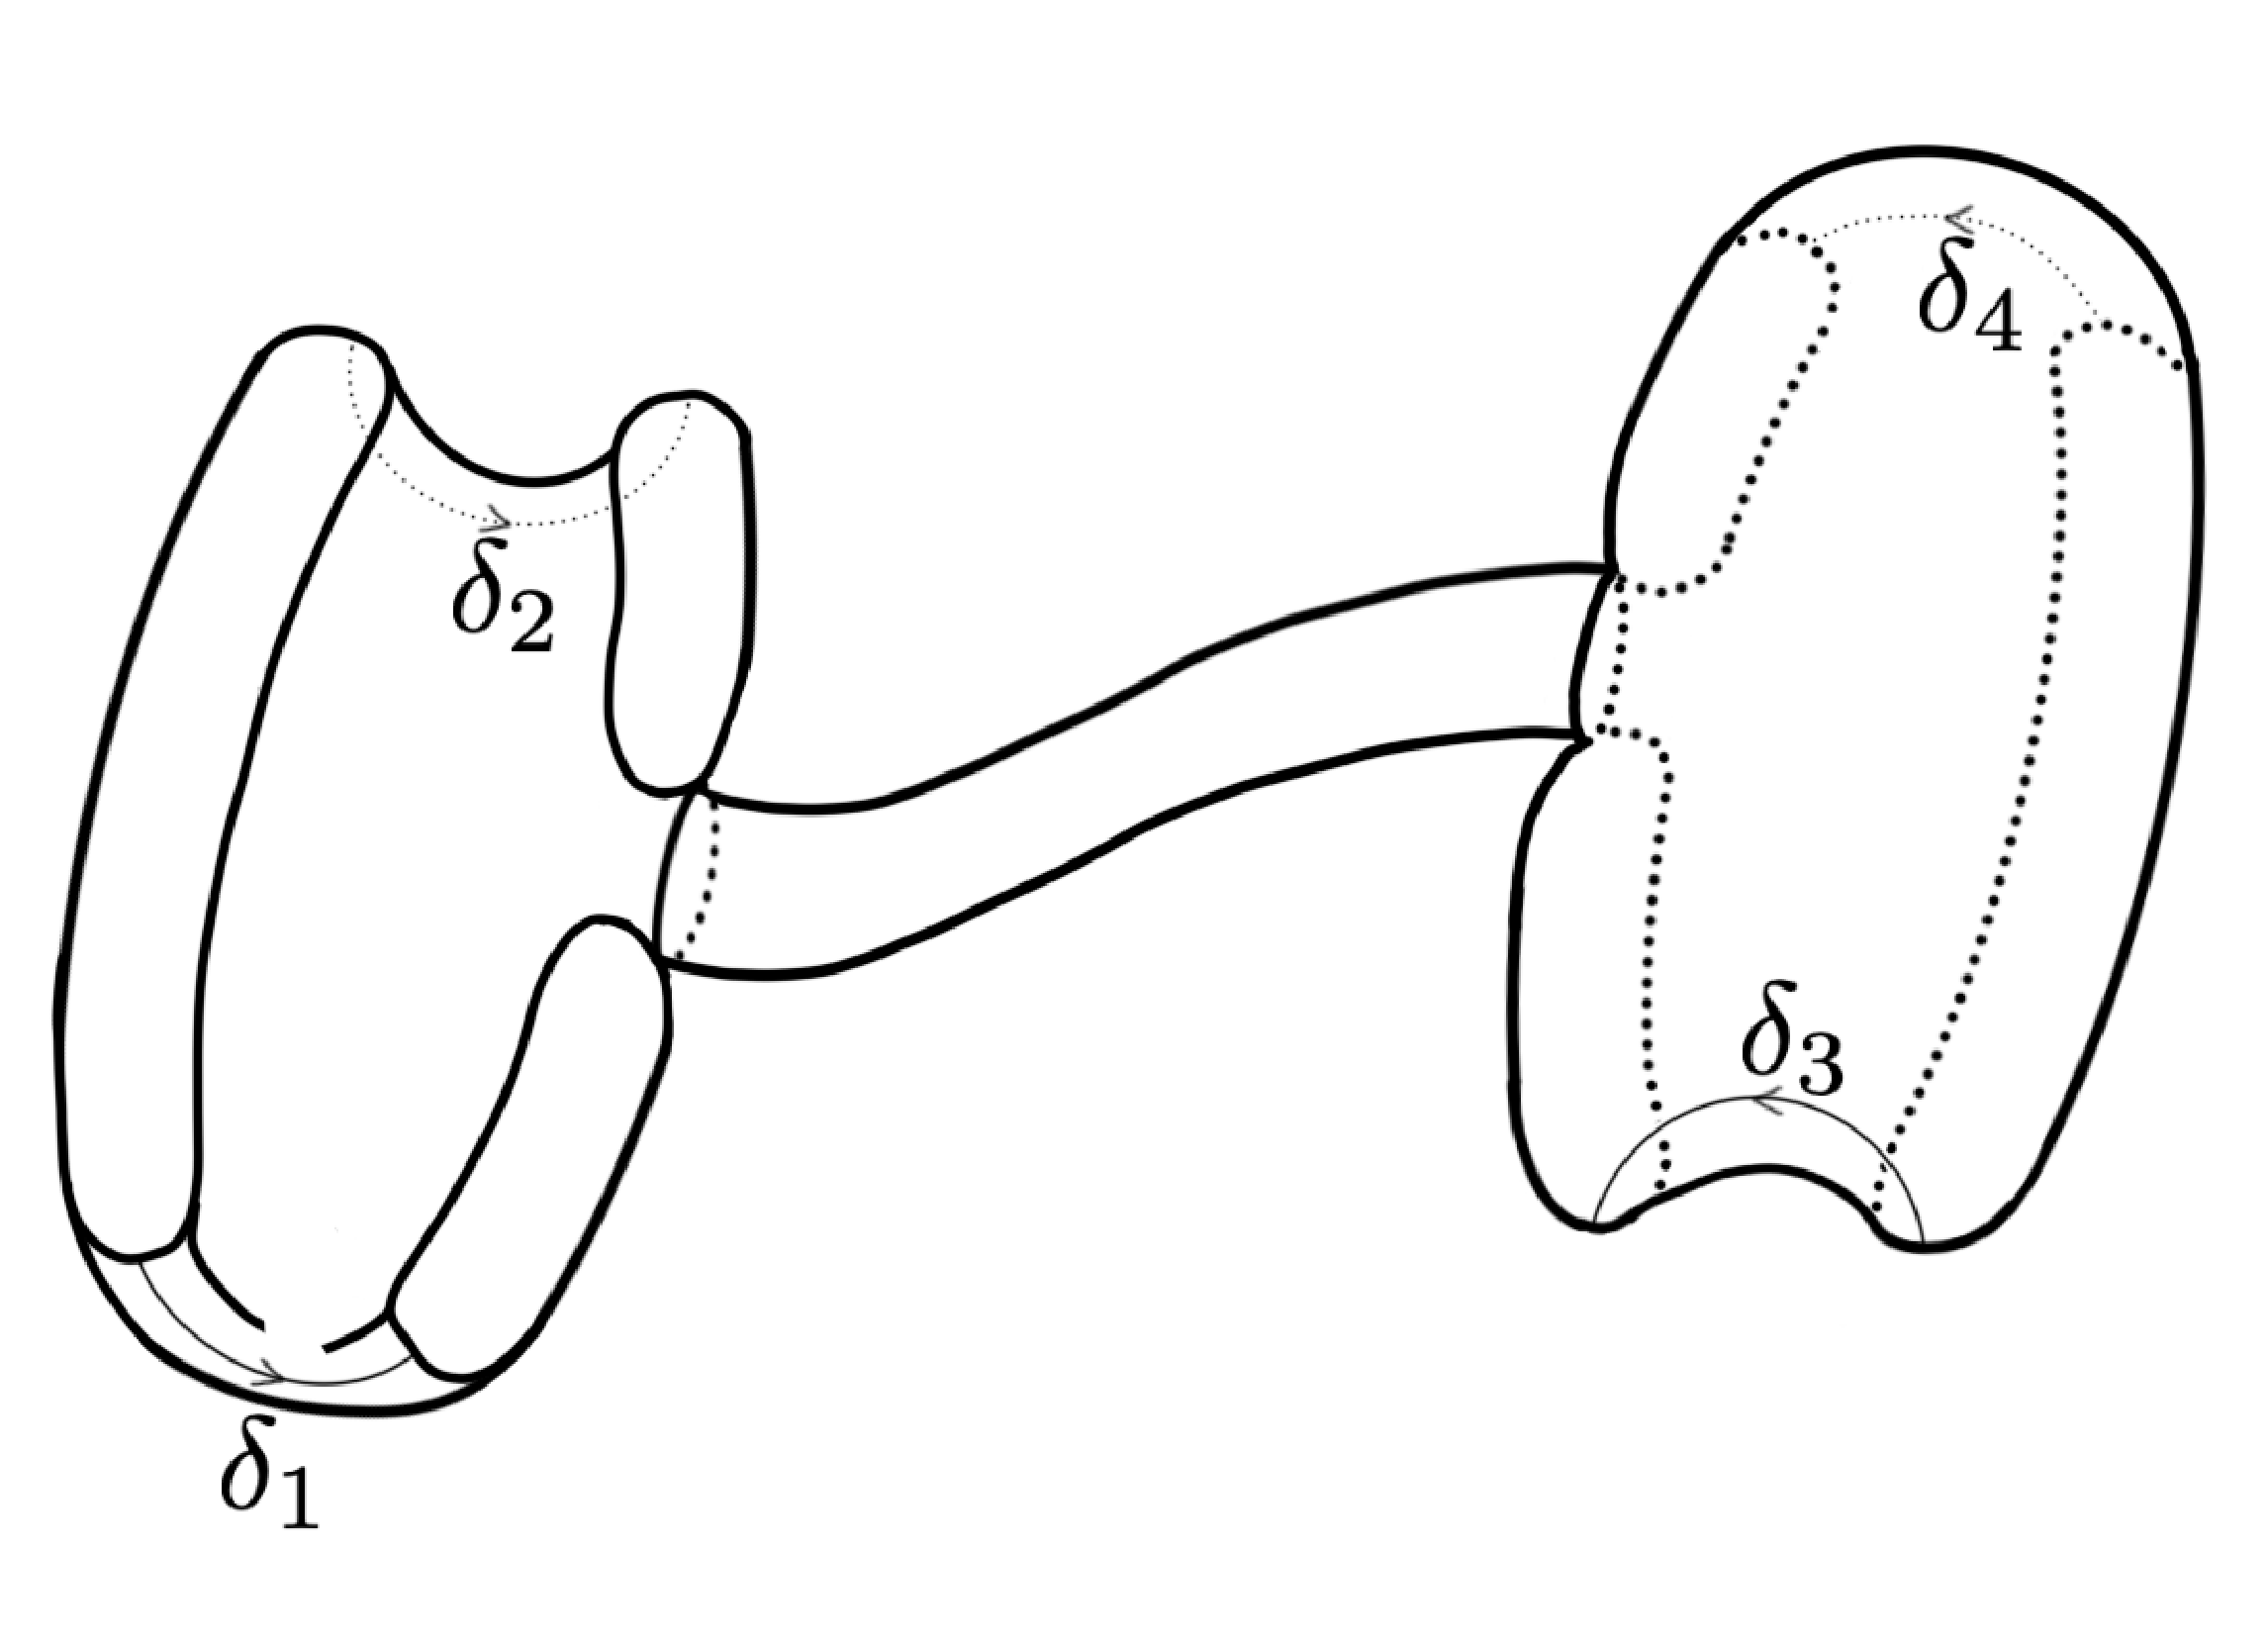
\includegraphics[scale=0.12]{images/ch4/section2/atoms/atom_5_half.pdf}
    \caption{Результат склейки $\widetilde{\Omega}_1 \cup \widetilde{\Omega}_2$ для перестройки 5.}
    \label{fig:pt9:_atom_5_half}
\endminipage\hfill
\end{figure}

Области $\widetilde{\Omega}_1$ и $\widetilde{\Omega}_2$ склеиваются по общим дугам на поверхности $\Xi = \const$, которые проектируются на граничные гиперболические дуги области $\widetilde{\Omega}$. Аналогично для областей $\widetilde{\Omega}_3$ и $\widetilde{\Omega}_4$. 
Те же пары областей также склеиваются по дугам, которые проектируются на горизонтальные отрезки $\Omega_{out} \cap \{y=0\}$. А именно, прообраз каждого из этих отрезков на поверхности $\Xi = \const$ эквивалентен окружности, половина дуги которого является общей границей областей $\Omega_{out, 1}^u, \Omega_{out, 2}^u, \Omega_{out, 1}^d, \Omega_{out, 2}^d$, а вторая половина дуги --- общая граница для областей $\Omega_{out, 3}^u, \Omega_{out, 4}^u, \Omega_{out, 3}^d, \Omega_{out, 4}^d$. 

Тогда склейка областей $\widetilde{\Omega}_1$ и $\widetilde{\Omega}_2$ по общим граничным дугам приводит к поверхности, изображенной на рис. \ref{fig:pt9:_atom_5_half}, край которой состоит из шести окружностей, которые проецируются на эллиптические граничные дуги области $\widetilde{\Omega}$ (см. рис. \ref{fig:pt9:_domain_atom_hyp_foc}). На склейке отметим дуги  $\delta_1, \ldots, \delta_4$, которые проецируются на горизонтальные отрезки $\Omega_{out} \cap \{y=0\}$.
Склейка областей $\widetilde{\Omega}_3 \cup \widetilde{\Omega}_4$ устроена аналогично. 

Для получения поверхности $\Xi = \const$ остается склеить $\widetilde{\Omega}_1 \cup \widetilde{\Omega}_2$ и $\widetilde{\Omega}_3 \cup \widetilde{\Omega}_4$ по общим граничным дугам, а также вдоль дуг $\delta_1, \ldots, \delta_4$. Поверхность $\Xi = \const$ до отождествления вдоль  $\delta_1, \ldots, \delta_4$ изображена на рис. \ref{fig:pt9:_atom_5}.

\begin{figure}[!htb]
\centering
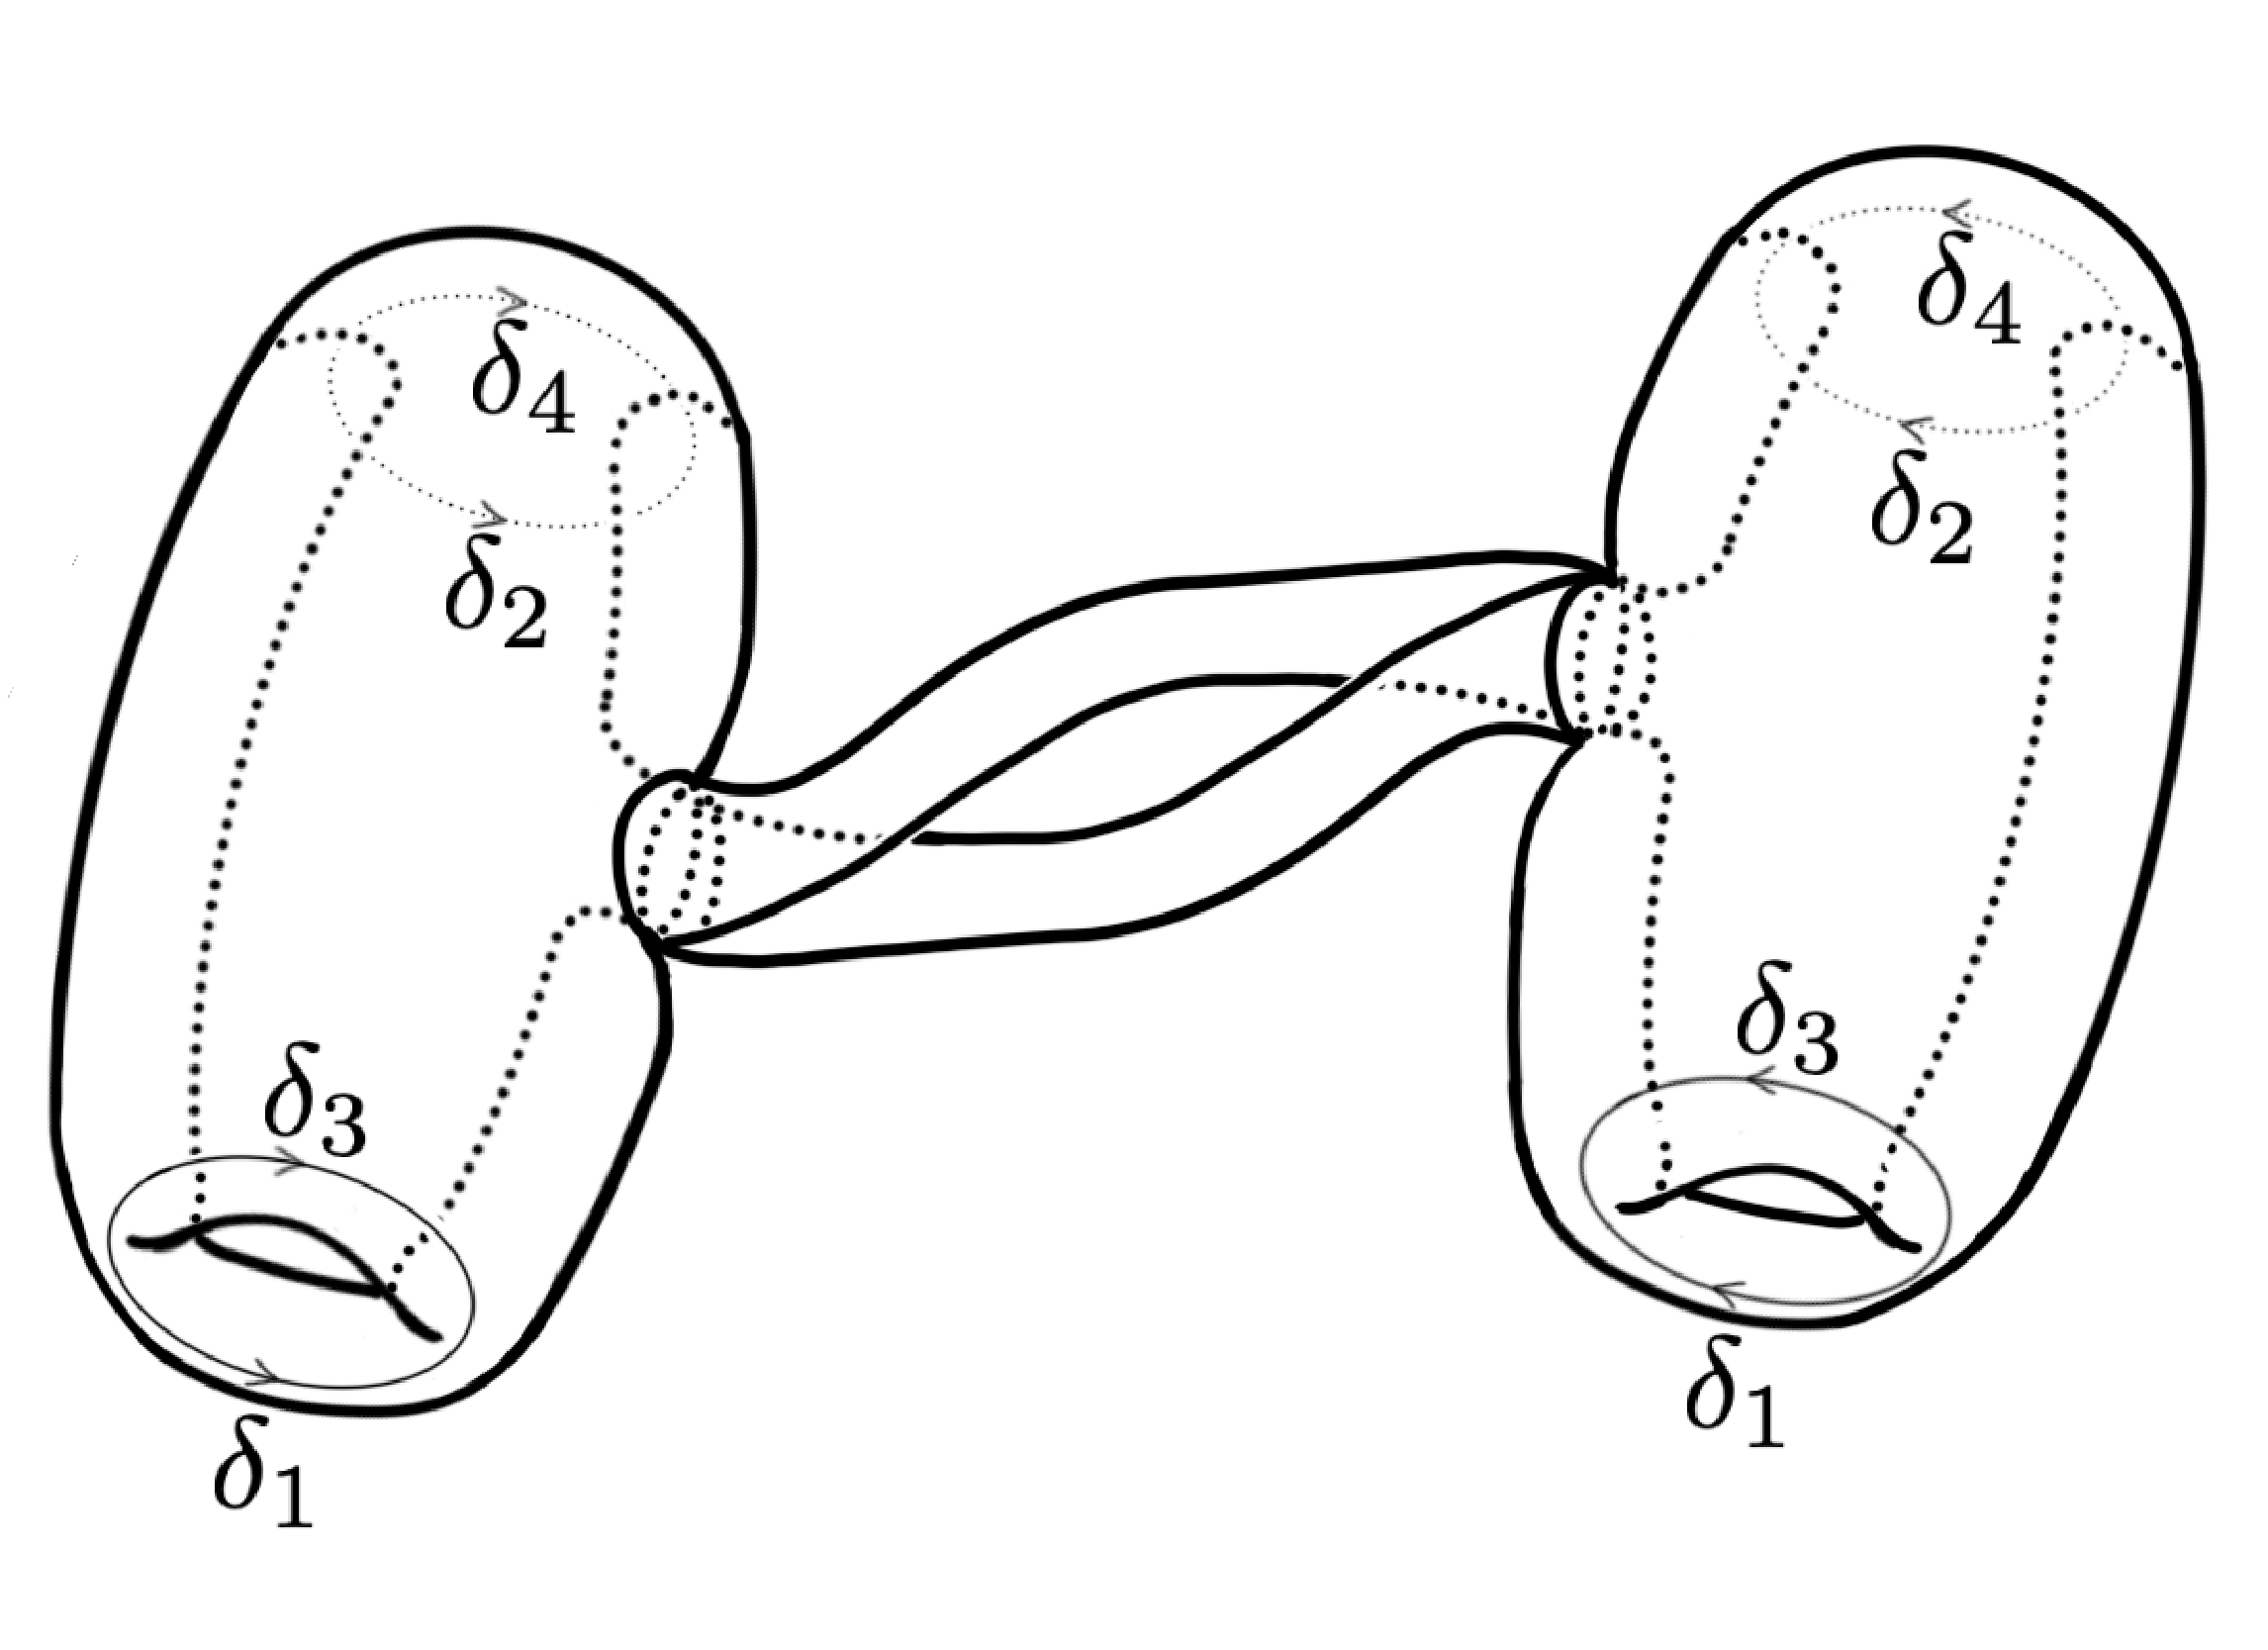
\includegraphics[scale=0.125]{images/ch4/section2/atoms/atom_5.pdf}
    \caption{Поверхность уровня $\Xi = \const$ для перестройки 5.}
    \label{fig:pt9:_atom_5}
\end{figure}


%На Рис. \ref{fig:pt9:_hyp_foc_atom} изображена поверхность для особого значения интеграла.
%Пунктирами изображены сечения <<ручек>>.
%\begin{figure}[!htb]
%\centering
%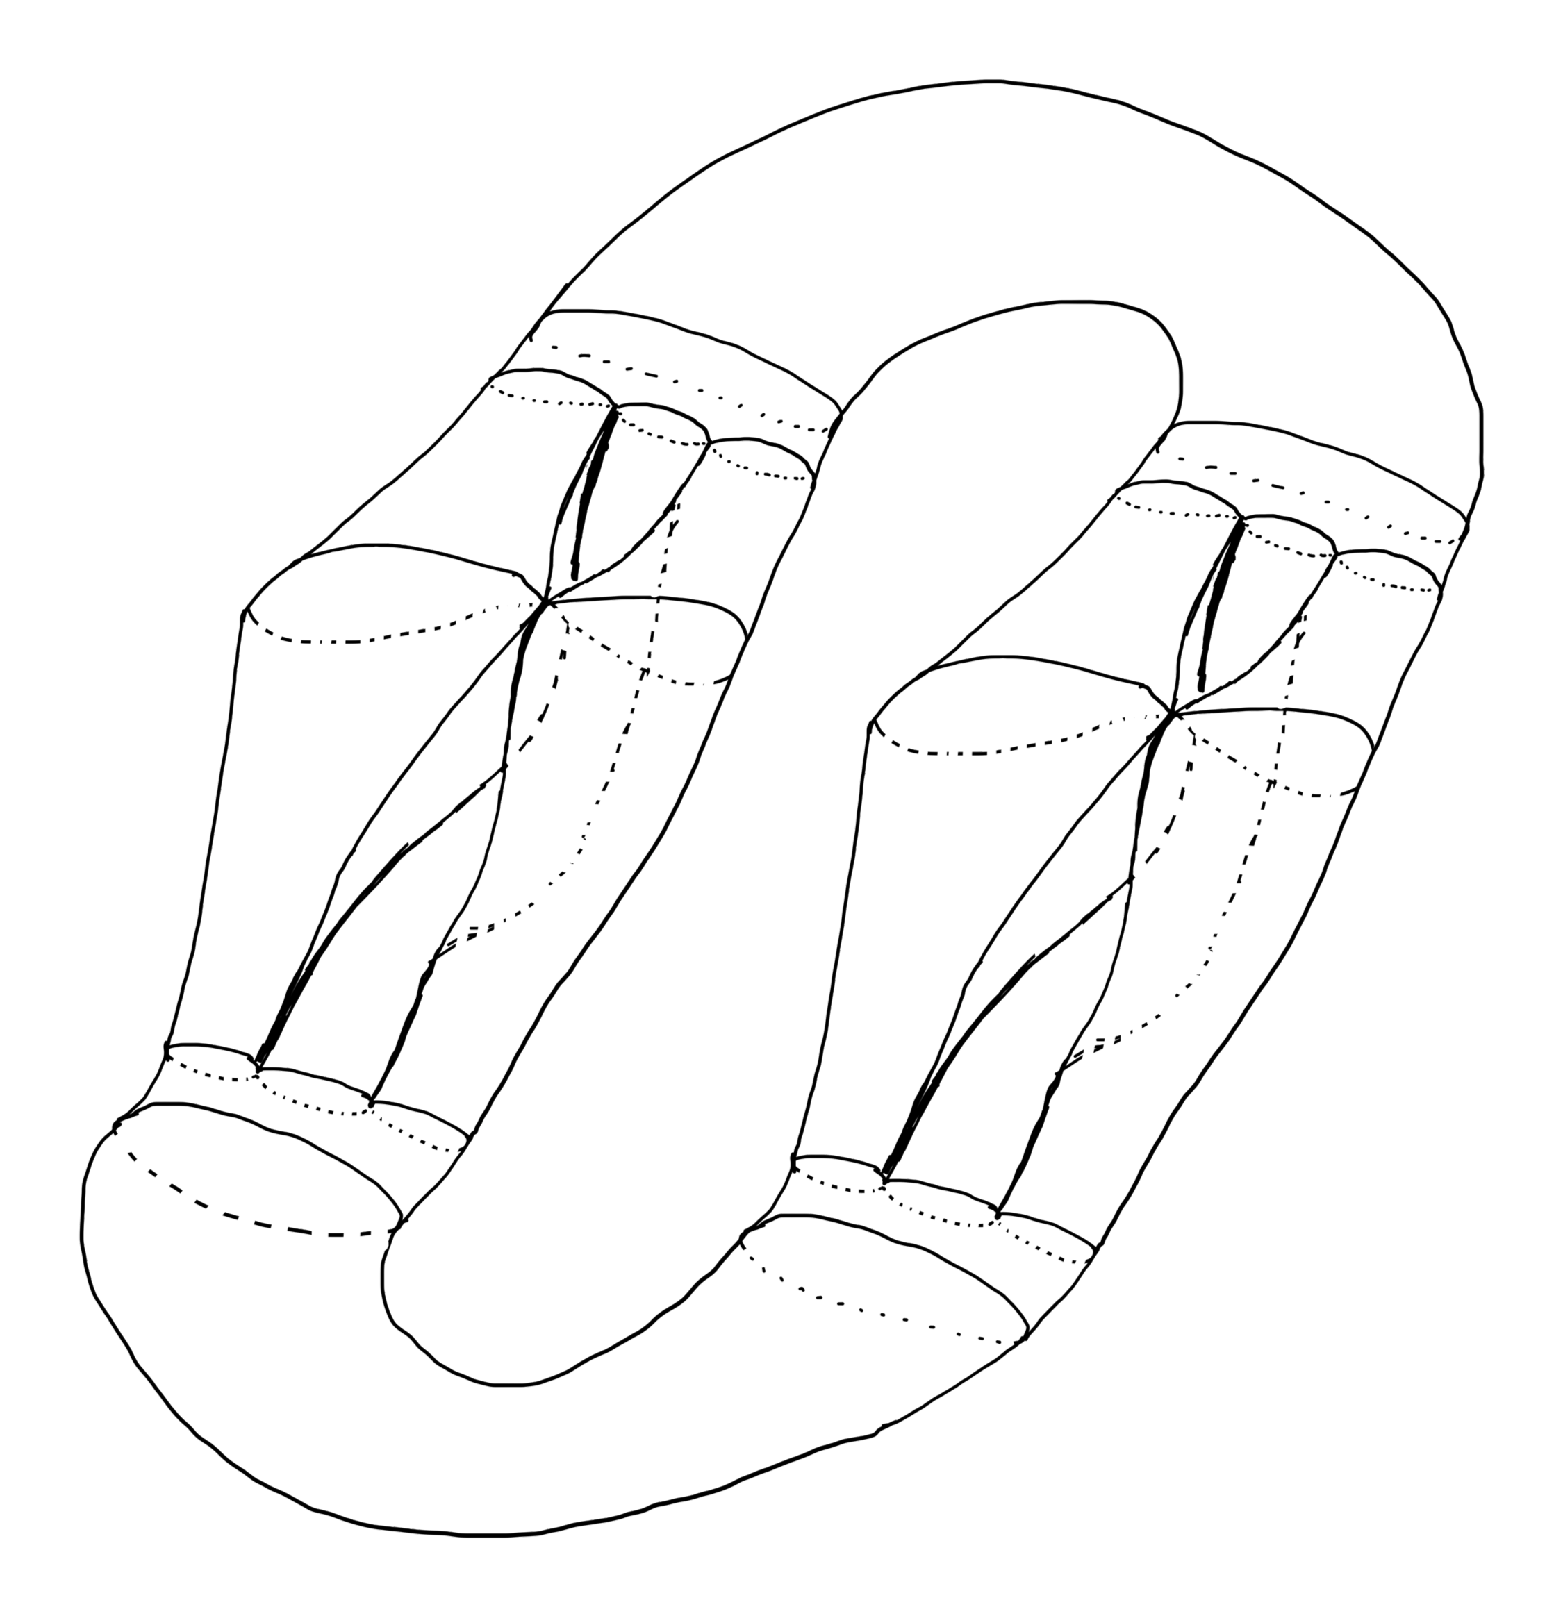
\includegraphics[scale=0.15]{images/ch4/section2/atoms/hyp_foc_atom.pdf}
%    \caption{Результирующая поверхность для особого значения $\Lambda=b^2 n_{out}^2$.}
%    \label{fig:pt9:_hyp_foc_atom}
%\end{figure}

\textbf{Перестройка 6.} 
Продолжения звеньев траектории, находящихся в области $\Omega_{out}$ касаются эллипса с параметром $\alpha_{out}$, а в области $\Omega_{in}$ сегменты траектории совпадают с вертикальной полуосью эллипса.

Поверхность $\Xi = \const$ можно представлять себе как предельный случай неособой поверхности, соответствующей случаю $D_1^6$, при $\alpha_{in} \to a^2$ (см. рис. \ref{fig:pt9:_diagramPlusIrregular}), когда две ручки схлопываются в две дуги, причем имеющие общие концы. 

Напомним рассуждения, проведенные нами для случая $D_1^6$. Рассмотрим склейку областей $\widetilde{\Omega}_1$ (см. рис. \ref{fig:pt9:_ell_and_hyp_2}) и $\widetilde{\Omega}_3$ (см. рис. \ref{fig:pt9:_ell_and_hyp2_permutations}) и аналогичную склейку областей $\widetilde{\Omega}_2$ и $\widetilde{\Omega}_4$.
Затем $\widetilde{\Omega}_1 \cup \widetilde{\Omega}_3$ и $\widetilde{\Omega}_2 \cup \widetilde{\Omega}_4$ склеиваются по тем граничным дугам, которые проецируются в эллиптические граничные дуги области $\widetilde{\Omega}$. Результатом склейки являются два тора, соединенные лентами (см. рис.  \ref{fig:pt9:_ell_and_hyp2_transformations}). Каждая лента ограничивается дугами, которые проецируются в граничные гиперболические дуги области $\widetilde{\Omega}$. 
%Граничные дуги ленты на листе $\widetilde{\Omega}_1$ отождествляются с одноименными дугами ленты $\widetilde{\Omega}_2$, результатом является цилиндр. Граничные окружности этого цилиндра проецируются в область $\widetilde{\Omega}$ в дуги эллипса с параметром $\lambda_1$, находящиеся между ветвями гиперболы с параметром $\alpha_{in}$. Аналогично для областей $\widetilde{\Omega}_3$ и $\widetilde{\Omega}_4$. 
%При устремлении параметра $\alpha_{in}$ к $a^2$ ширина всех четырех лент устремляется к нулю, то есть ручка, полученная склейкой области $\widetilde{\Omega}_1$ с $\widetilde{\Omega}_2$ превращается в кривую, которая соединяет верхнюю и нижнюю вершины эллипса с параметром $\lambda_1$. Аналогично для областей $\widetilde{\Omega}_3$ и $\widetilde{\Omega}_4$.
%Поверхность уровня $\Xi = \const$ изображена на рис. \ref{fig:pt9:_atom_6} и представляет собой два тора, соприкасающихся по двум соединенным окружностью точкам.
Области $\widetilde{\Omega}_1$ и $\widetilde{\Omega}_2$ отождествляются по общим границам, проектирующимся на левую и правую ветви гиперболы $Q_{\alpha_{in}}$ в области $\Omega_{in}$. 

В момент перестройки ручка, образованная склейкой областей $\widetilde{\Omega}_1$ и $\widetilde{\Omega}_2$ (соответственно, $\widetilde{\Omega}_3$ и $\widetilde{\Omega}_4$) стягивается в кривую. 
То есть поверхность $\Xi = \const$ представляет собой два касающихся в двух точках тора, при этом обе общие точки этих двух торов соединены двумя кривыми, см. рис. \ref{fig:pt9:_atom_6}.
\begin{figure}[!htb]
\centering
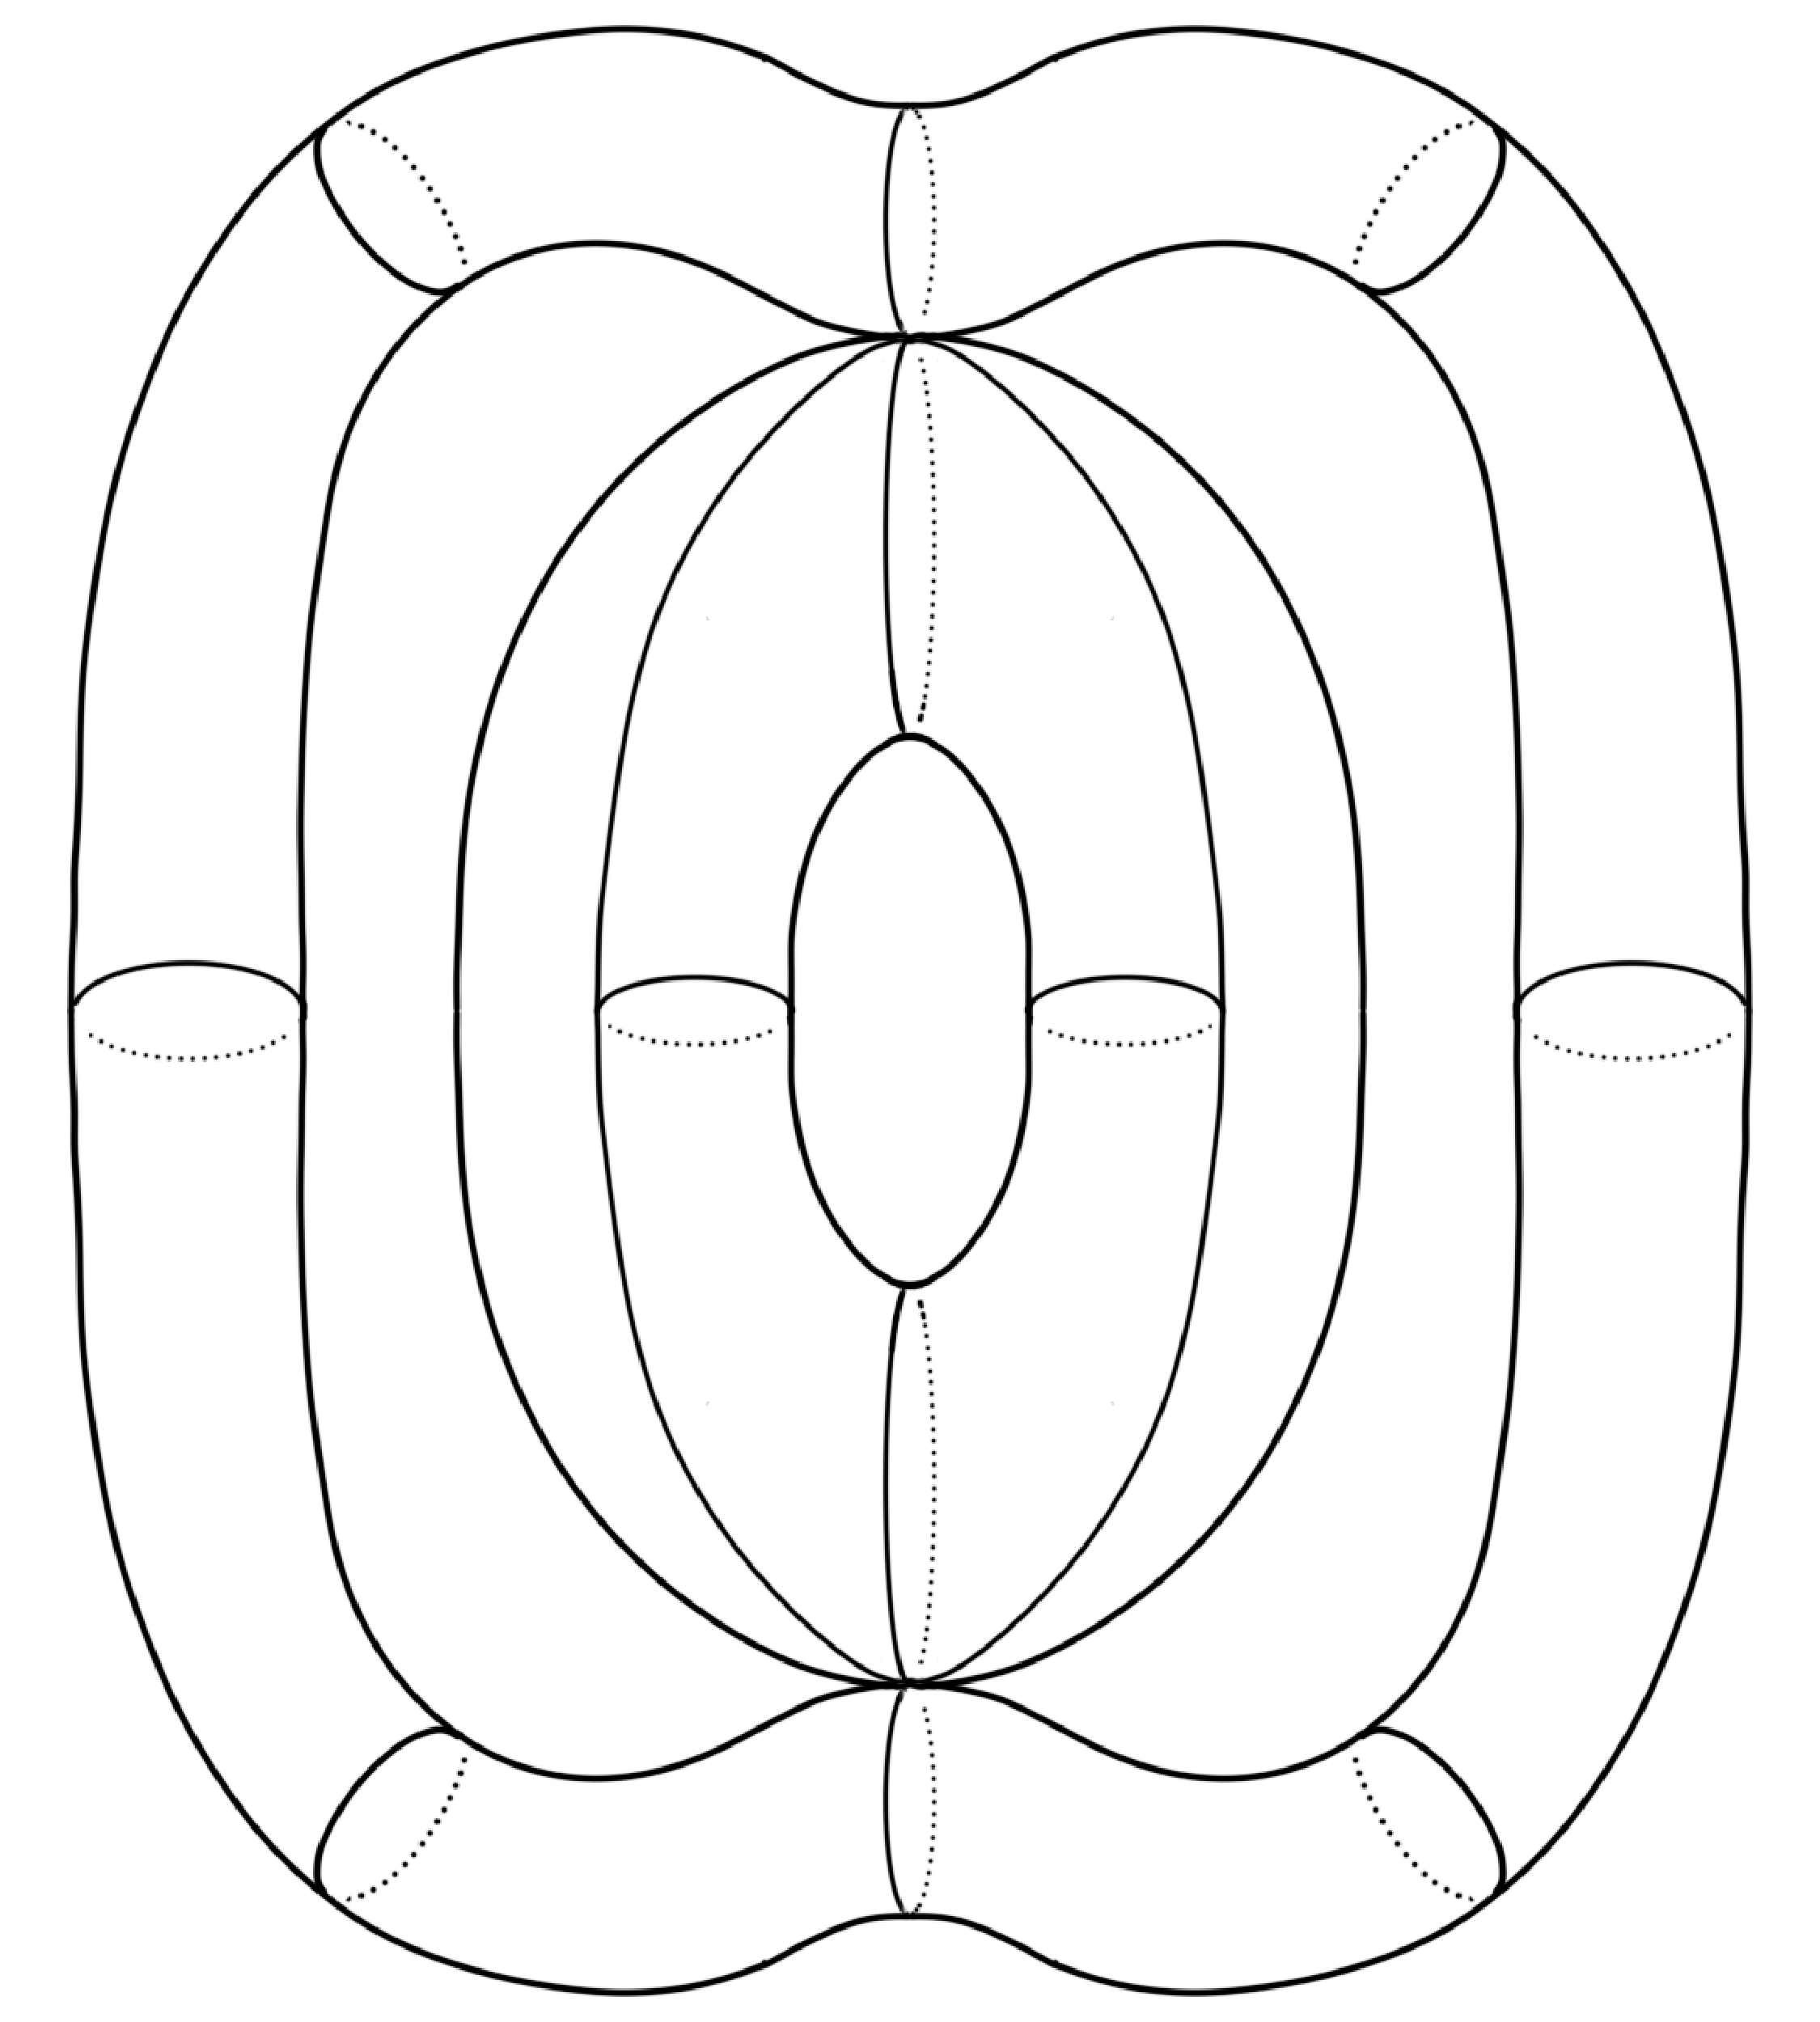
\includegraphics[scale=0.09]{images/ch4/section2/atoms/atom_6.pdf}
    \caption{Поверхность уровня $\Xi = \const$ для перестройки 6.}
    \label{fig:pt9:_atom_6}
\end{figure}


\textbf{Перестройка 7.}
Сегменты бильярдной траектории в области $\Omega_{in}$ лежат на проходящих через фокусы прямых, не заходя при этом в область $\Omega_{out}$.

Положим $\widetilde{\Omega} = \Omega_{in}$. Проекция $\pi$ четырехлистна в любой внутренней точке $\widetilde{\Omega} \setminus \{y=0\}  = (\Omega_{in} \cap \{y>0\}) \cup (\Omega_{in} \cap \{y<0\}) = \Omega_{in}^u \cup \Omega_{in}^d$.
Тогда последние две области имеют на поверхности $\Xi = \const$ по четыре прообраза $\Omega_{in, j}^u, \Omega_{in, j}^d, j=1, \ldots, 4$, которые занумерованы в соответствии с правилом \eqref{eq:foc_numeration}.

На поверхности $\Xi = \const$ общая граничная дуга областей $\Omega_{in, 1}^u, \Omega_{in, 4}^u$ проецируется на дугу эллипса с параметром $\lambda_1$ в верхней полуплоскости. Аналогично для областей $\Omega_{in, 2}^u, \Omega_{in, 3}^u$. На симметричную дугу эллипса с параметром $\lambda_1$ проецируются граничные дуги для $\Omega_{in, 1}^d$ и $\Omega_{in, 4}^d$, аналогично для областей $\Omega_{in, 2}^d, \Omega_{in, 3}^d$. 
В соединяющий фокусы отрезок горизонтальной прямой проецируются общие граничные дуги областей $\Omega_{in, 1}^u, \Omega_{in, 4}^u, \Omega_{in, 1}^d, \Omega_{in, 4}^d$. Аналогично для областей $\Omega_{in, 2}^u, \Omega_{in, 3}^u, \Omega_{in, 2}^d$ и $\Omega_{in, 3}^d$.

Определим области 
\begin{equation}
\begin{array}{cc}
\widetilde{\Omega}_1 = \Omega_{in, 1}^u \cup \Omega_{in, 4}^d, &
\widetilde{\Omega}_2 = \Omega_{in, 2}^u \cup \Omega_{in, 3}^d, \\
\widetilde{\Omega}_3 = \Omega_{in, 3}^u \cup \Omega_{in, 2}^d, &
\widetilde{\Omega}_4 = \Omega_{in, 4}^u \cup \Omega_{in, 1}^d.
\end{array}
\label{eq:case7Omegas}
\end{equation}

Склеим области $\widetilde{\Omega}_1$ и $\widetilde{\Omega}_4$ по общим граничным областям, которые проецируются на эллиптические граничные дуги области $\widetilde{\Omega}$, а также по общей дуге, которая проецируется на соединяющие фокусы отрезок.
Аналогично склеим области $\widetilde{\Omega}_2$ и $\widetilde{\Omega}_3$. Результатами склеек являются два цилиндра с восьмерками в поперечных сечениях каждого.

Окружности, ограничивающие восьмерки на левом и правом торцах цилиндров, проецируются в левый и правый отрезки $\Omega_{in} \cap \{y=0\}$.
На этих отрезках отождествляются области $\Omega_{in, 1}^u$ и $\Omega_{in, 2}^d$. Аналогично для областей $\Omega_{in, 2}^u$ и $\Omega_{in, 1}^d$, для $\Omega_{in, 3}^u$ и $\Omega_{in, 4}^d$, а также $\Omega_{in, 4}^u$ и $\Omega_{in, 3}^d$.
Тогда на правом отрезке $\Omega_{in} \cap \{y=0\}$ \textit{верхняя} граничная окружность склейки $\widetilde{\Omega}_1 \cup \widetilde{\Omega}_4$ склеивается с  \textit{нижней} граничной окружностью склейки $\widetilde{\Omega}_2 \cup \widetilde{\Omega}_3$, а \textit{нижняя} окружность на  $\widetilde{\Omega}_1 \cup \widetilde{\Omega}_4$ --- с \textit{верхней} на $\widetilde{\Omega}_2 \cup \widetilde{\Omega}_3$. Аналогично на левом отрезке $\Omega_{in} \cap \{y=0\}$.

Таким образом, два цилиндра с восьмерками в сечении склеиваются в один тор с восьмеркой в сечении, образуя поверхность $\Xi = \const$.

\textbf{Перестройка 8.} 
Звенья траектории в области $\Omega_{in}$ касаются гиперболы с параметром $\alpha_{in}$, а в области $\Omega_{out}$ совпадают вертикальной полуосью граничного эллипса.

Поверхность $\Xi = \const$ можно представлять себе как предельный случай неособой поверхности, соответствующей случаю $D_1^2$, при $\alpha_{out} \to a^2$ (см. рис. \ref{fig:pt9:_diagramPlusIrregular}), когда две ручки схлопываются в окружности.

Напомним рассуждения, проведенные нами для случая $D_1^2$. Рассмотрим склейку областей $\widetilde{\Omega}_1$ (см.  рис. \ref{fig:pt9:_img17}) и $\widetilde{\Omega}_4$  по общим границам, которые проецируются в эллиптические граничные дуги области $\widetilde{\Omega}$ и аналогичную склейку областей $\widetilde{\Omega}_2$ и $\widetilde{\Omega}_3$.
Результатом склейки является сфера с шестью дырками, при этом каждая дырка ограничивается парой дуг на поверхности $\Xi=\const$, которые проецируются в граничные гиперболические дуги области $\widetilde{\Omega}$. 
Части границ областей $\widetilde{\Omega}_1$ и $\widetilde{\Omega}_2$ отождествляются по дугам, которые проектируются в часть границы области $\widetilde{\Omega}$, аналогично для областей $\widetilde{\Omega}_3$ и $\widetilde{\Omega}_4$.

На рис. \ref{fig:pt9:_atom_8_step} изображен результат склейки $\widetilde{\Omega}_1 \cup \widetilde{\Omega}_4$. Его границей являются три пары окружностей, по которым приклеивается поверхность, полученная в результате аналогичной склейки $\widetilde{\Omega}_2 \cup \widetilde{\Omega}_3$. 

В момент перестройки две верхние (соответственно, две нижние) граничные окружности $\widetilde{\Omega}_1 \cup \widetilde{\Omega}_4$ схлопываются в одну окружность. 

Таким образом, поверхность $\Xi = \const$ представляет собой тор, на котором отмечены две пары отождествленных точек, при этом из точек, полученных в результате отождествления, <<растет>> по одной окружности, см. рис. \ref{fig:pt9:_atom_8}.

%\begin{figure}[!htb]
%\minipage{0.33\textwidth}
%\centering
%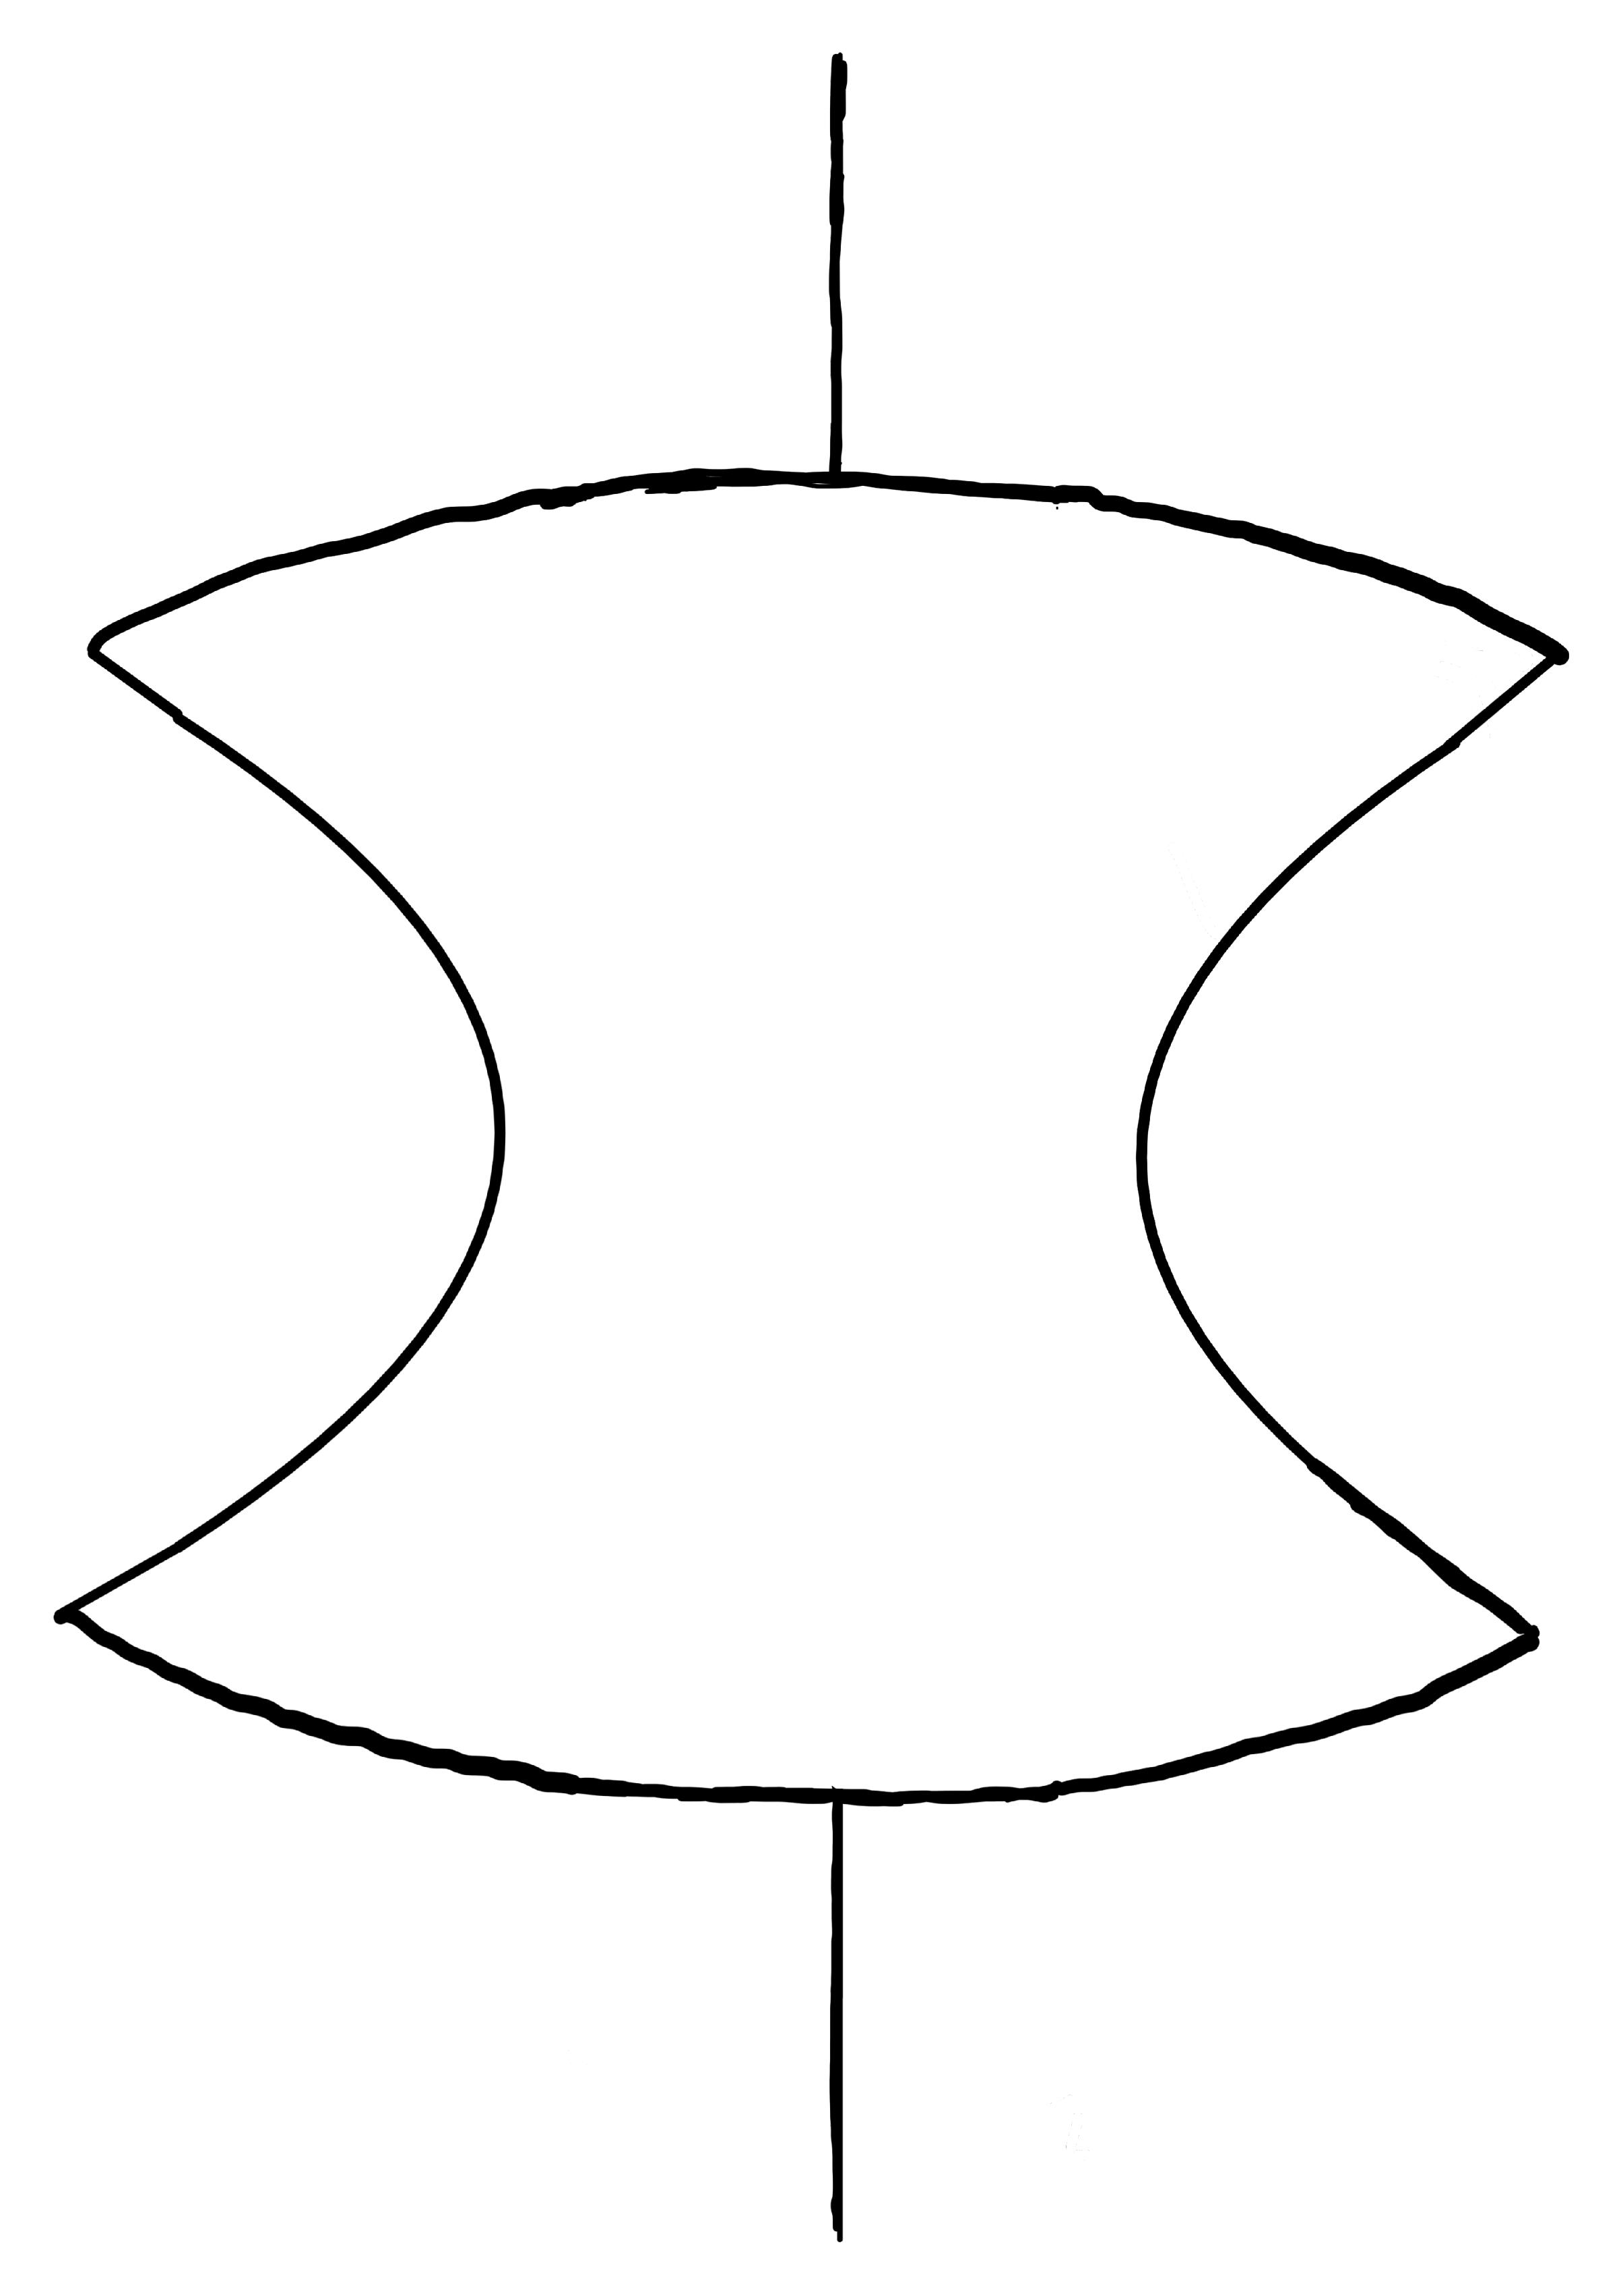
\includegraphics[scale=0.07]{images/ch4/section2/atoms/domain_atom_hyp_void.pdf}
%    \caption{Соответствующая случаю 8 область $\Omega$.}
%    \label{fig:pt9:_domain_atom_hyp_void}
%\endminipage\hfill
%\minipage{0.32\textwidth}
%\centering
%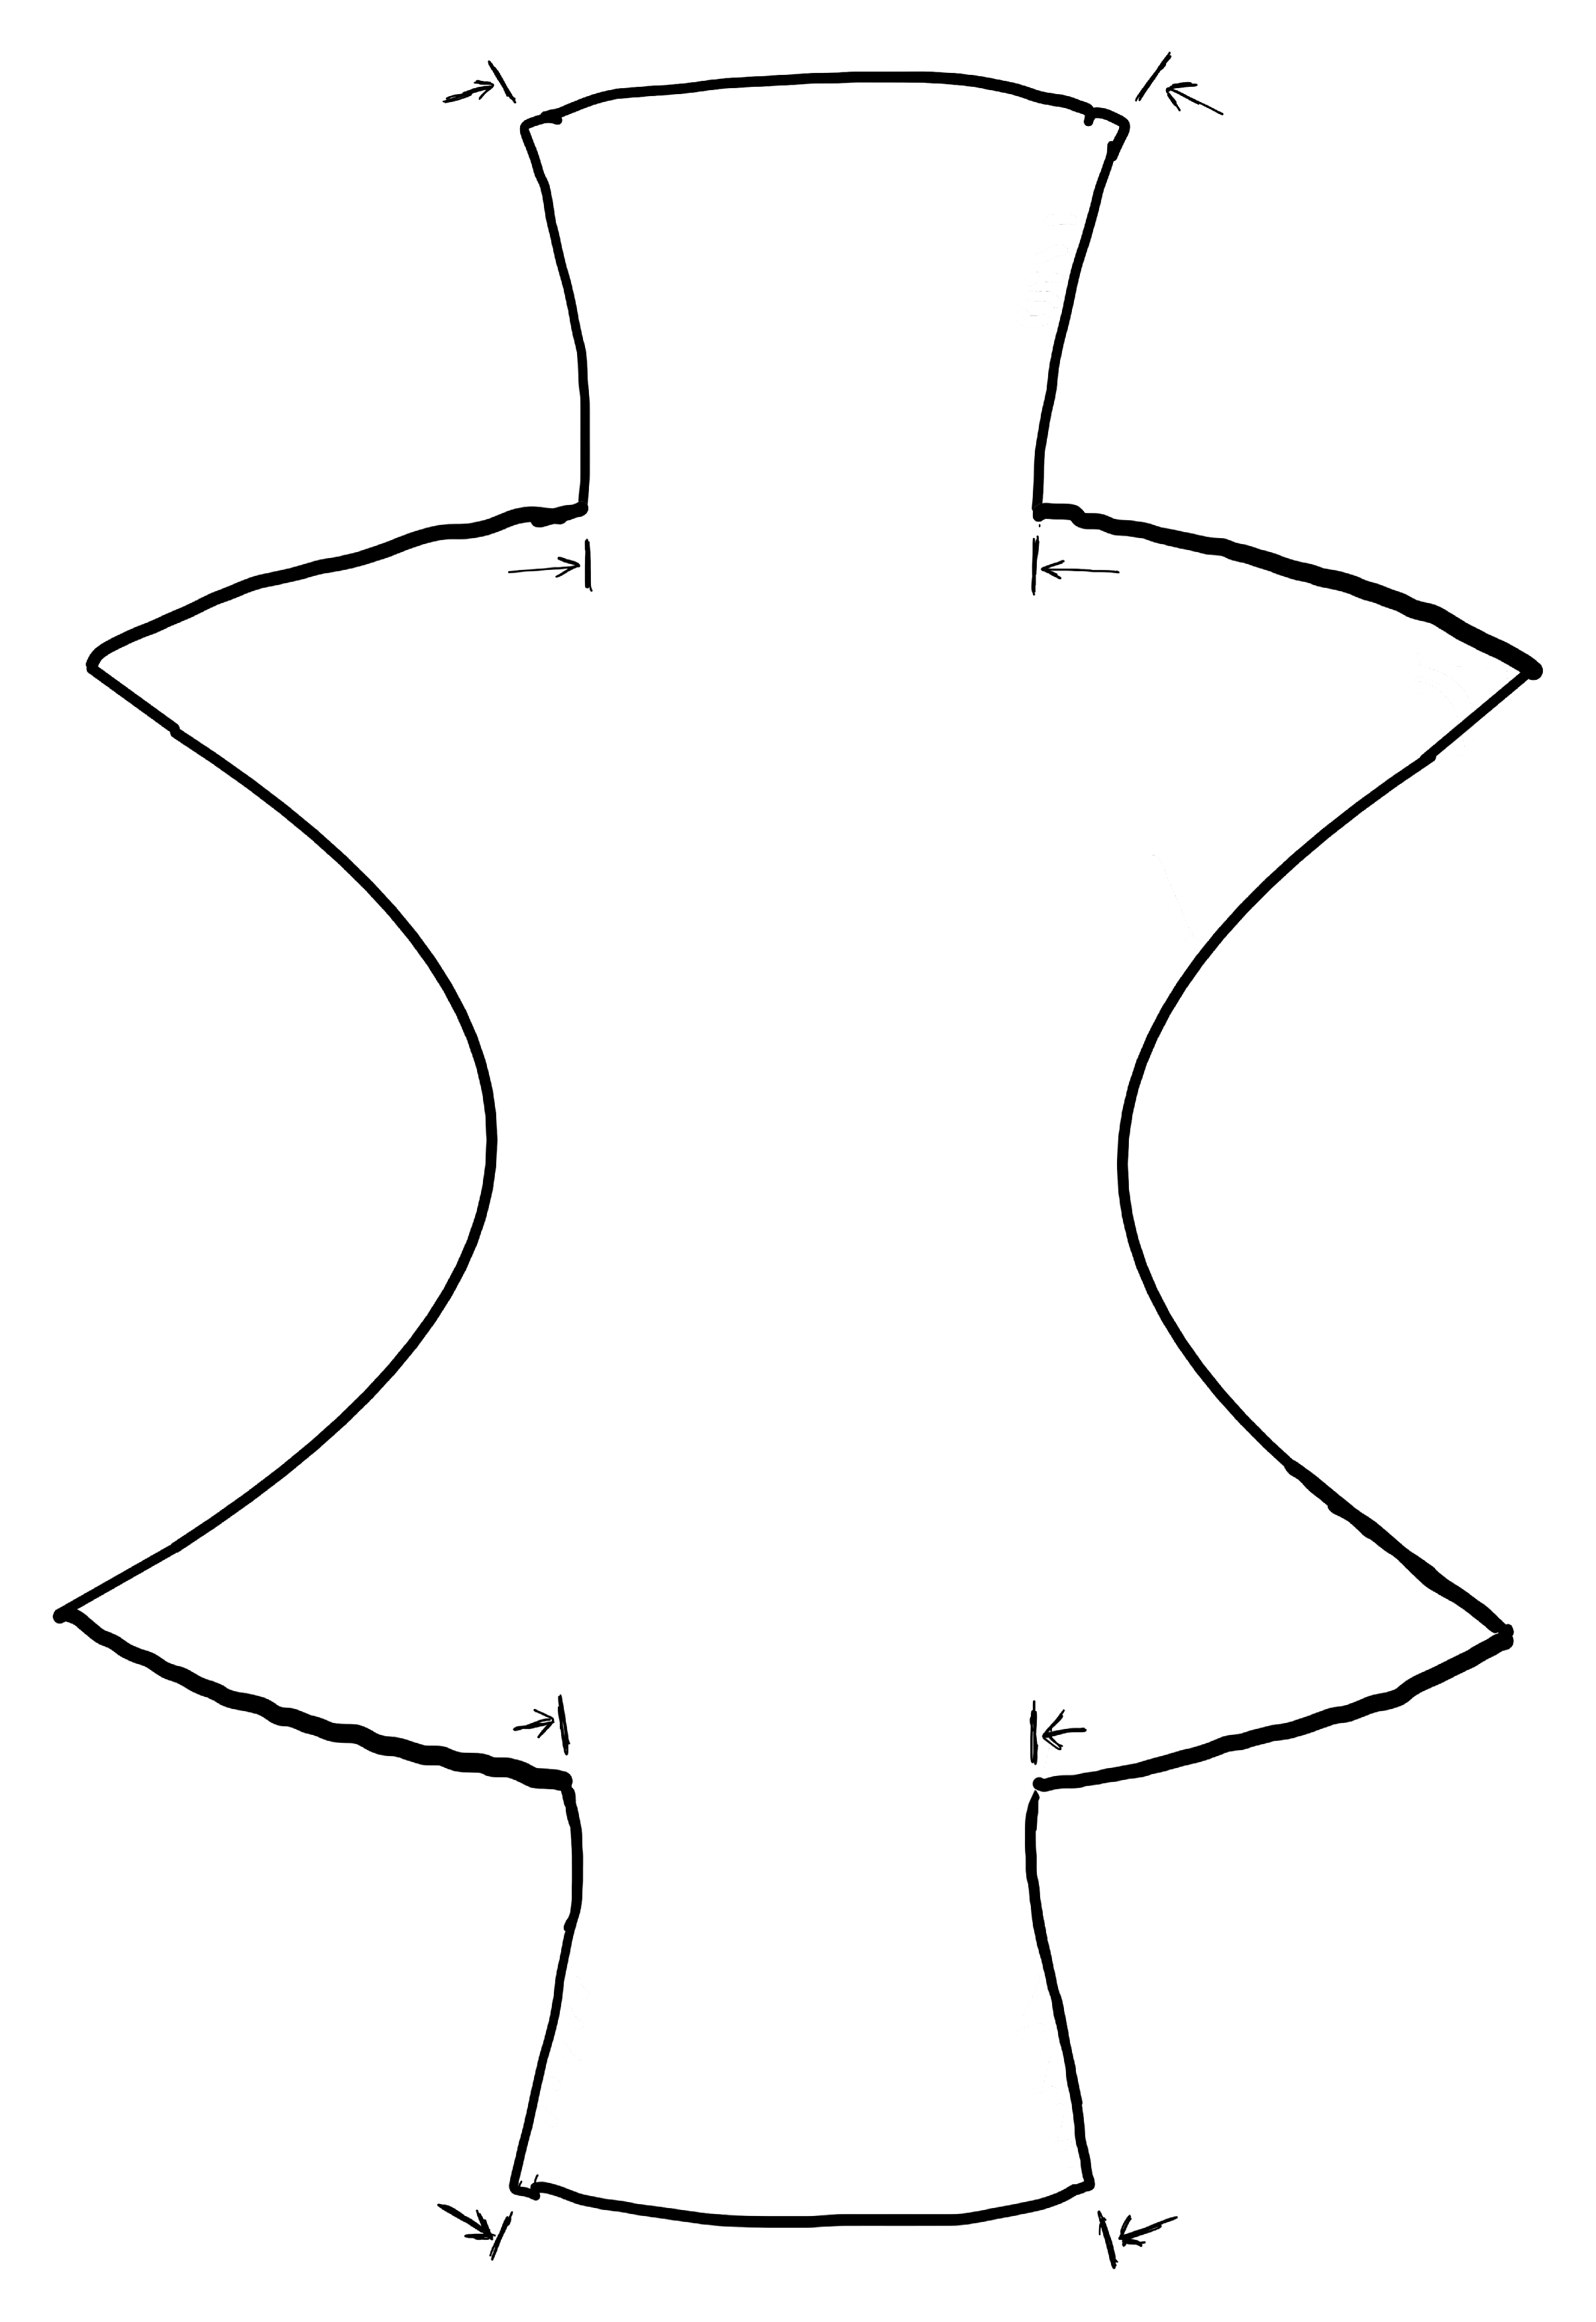
\includegraphics[scale=0.07]{images/ch4/section2/atoms/domain_atom_hyp_void_before_limit.pdf}
%    \caption{Область $\Omega$ как предельный случай.}
%    \label{fig:pt9:_domain_atom_hyp_void_before_limit}
%\endminipage\hfill
%\minipage{0.3\textwidth}
%\centering
%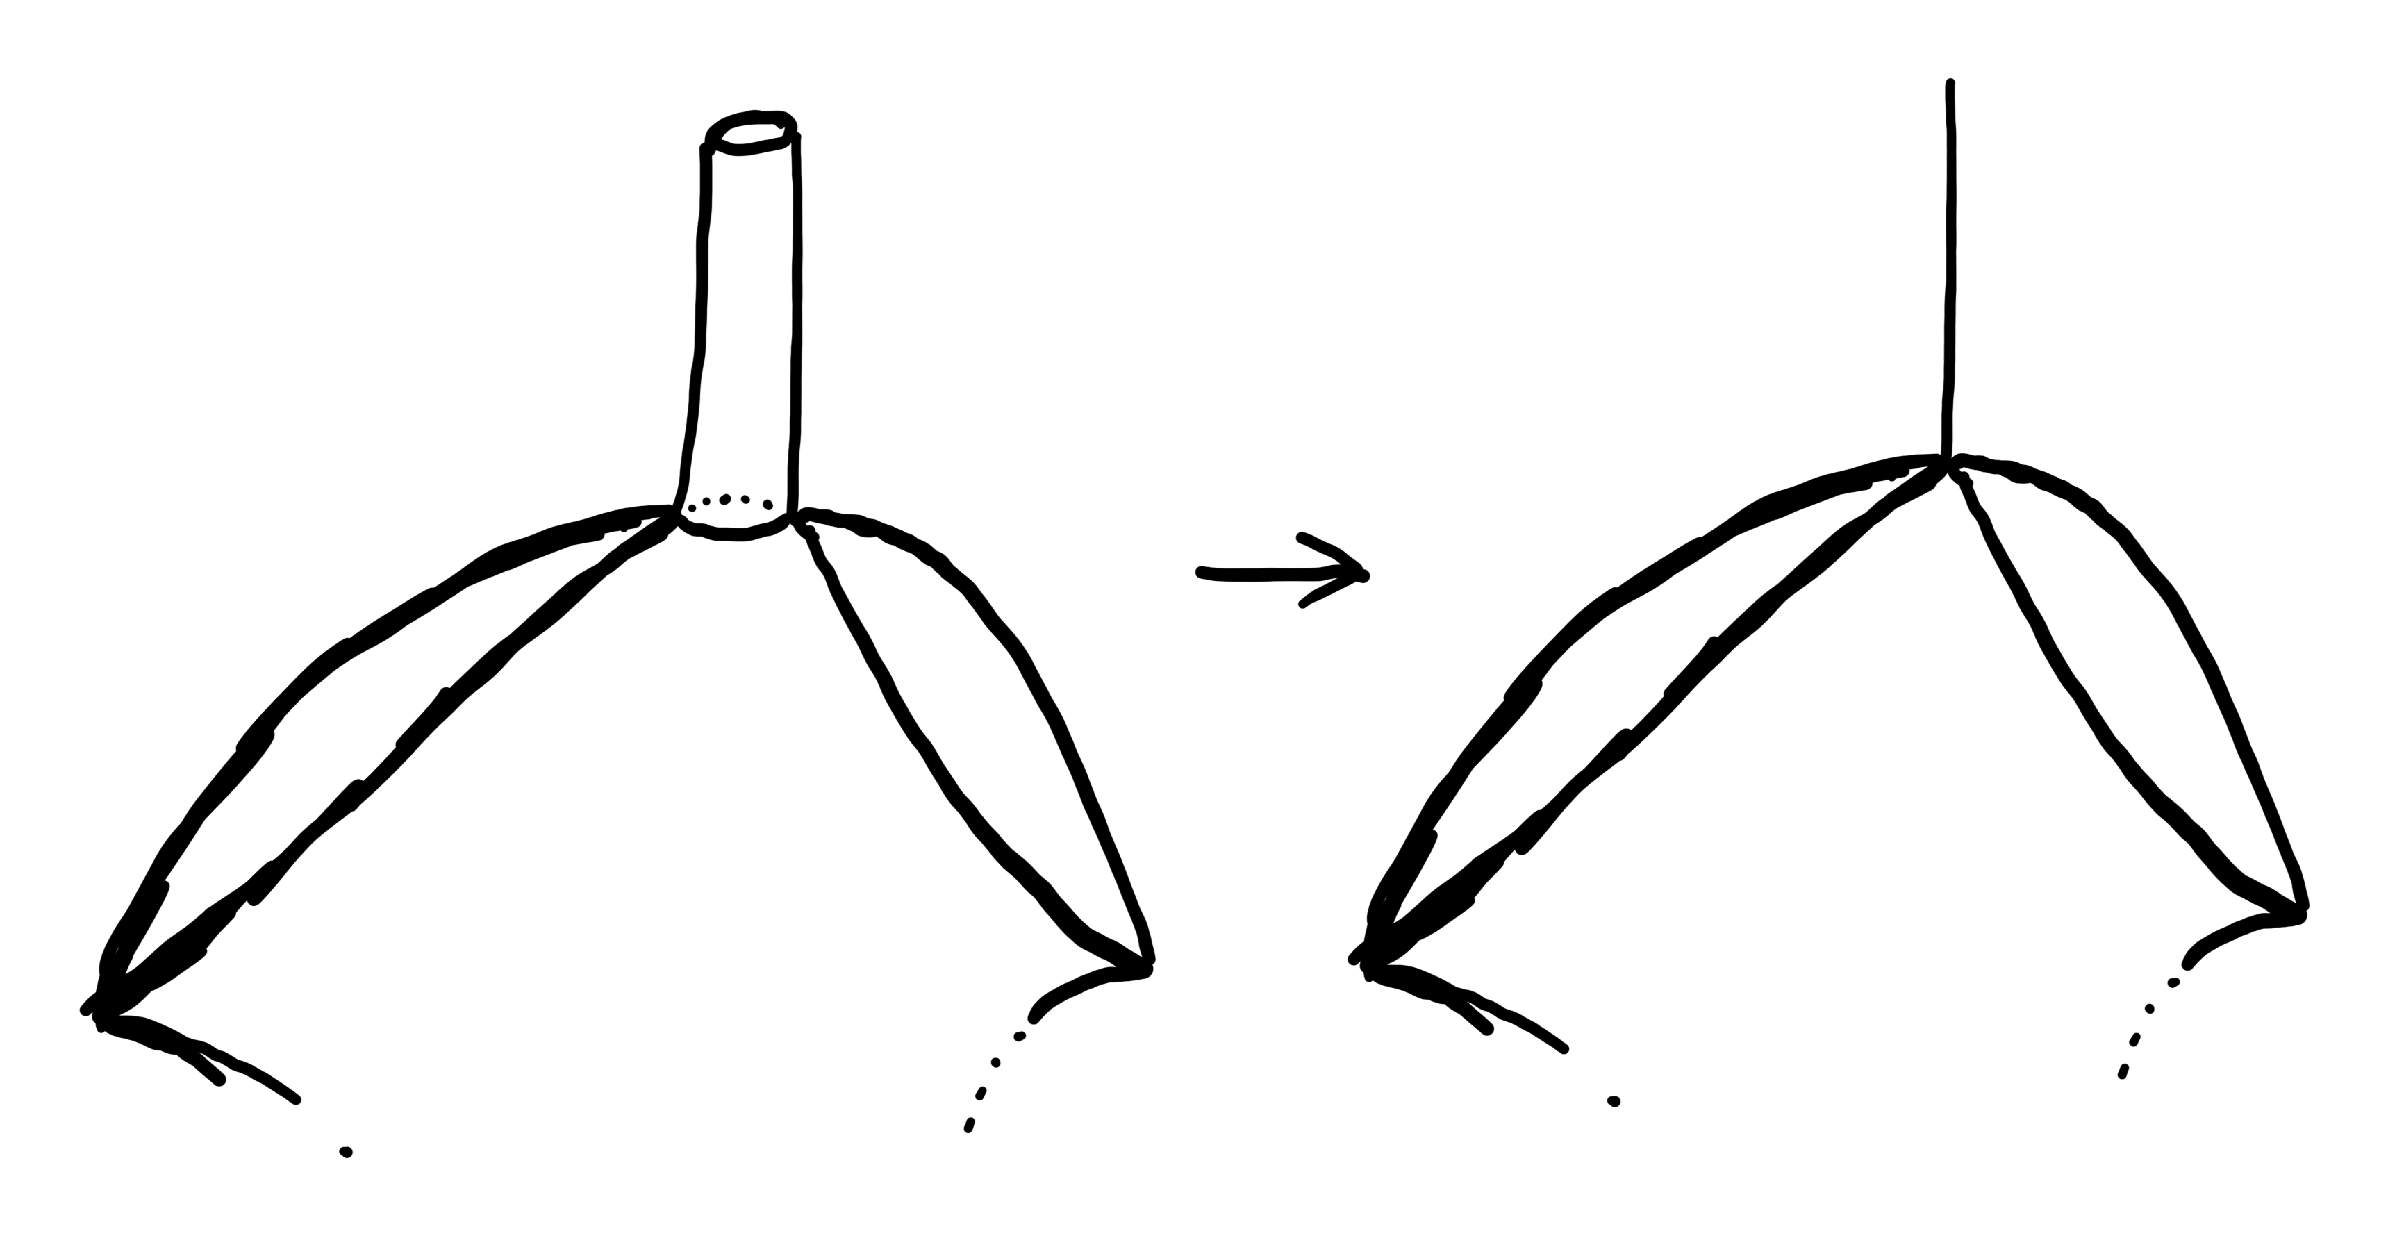
\includegraphics[scale=0.1]{images/ch4/section2/atoms/atom_hyp_void_iter1.pdf}
%    \caption{Схлопывание одной из ручек.}
%    \label{fig:pt9:_atom_hyp_void_iter1}
%\endminipage\hfill
%\end{figure}
%
%Для того, чтобы получить сам атом, остается провести склейку как показано на Рис. \ref{fig:pt9:_atom_hyp_void_iter2}, результат которой можно увидеть на Рис. \ref{fig:pt9:_hyp_void_atom}.
%
\begin{figure}[!htb]
\minipage{0.5\textwidth}
\centering
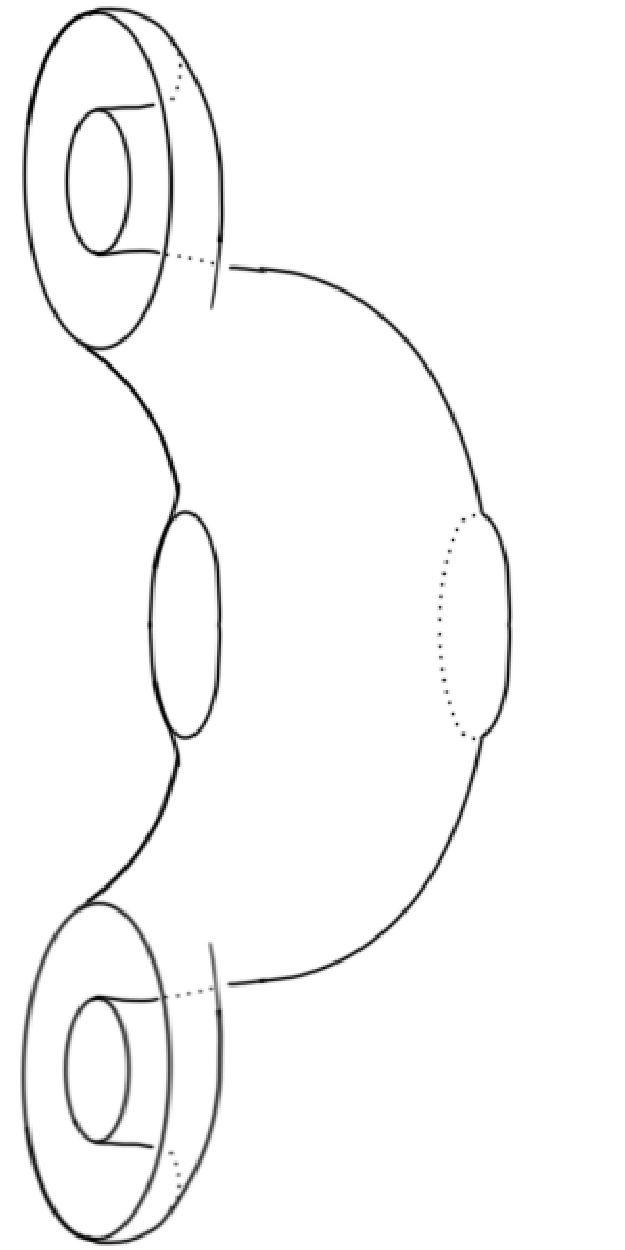
\includegraphics[width=2.5cm]{images/ch4/section2/atoms/atom_8_step.pdf}
    \caption{Результат склейки $\widetilde{\Omega}_1 \cup \widetilde{\Omega}_4$ для перестройки 8.}
    \label{fig:pt9:_atom_8_step}
\endminipage\hfill
\minipage{0.5\textwidth}
\centering
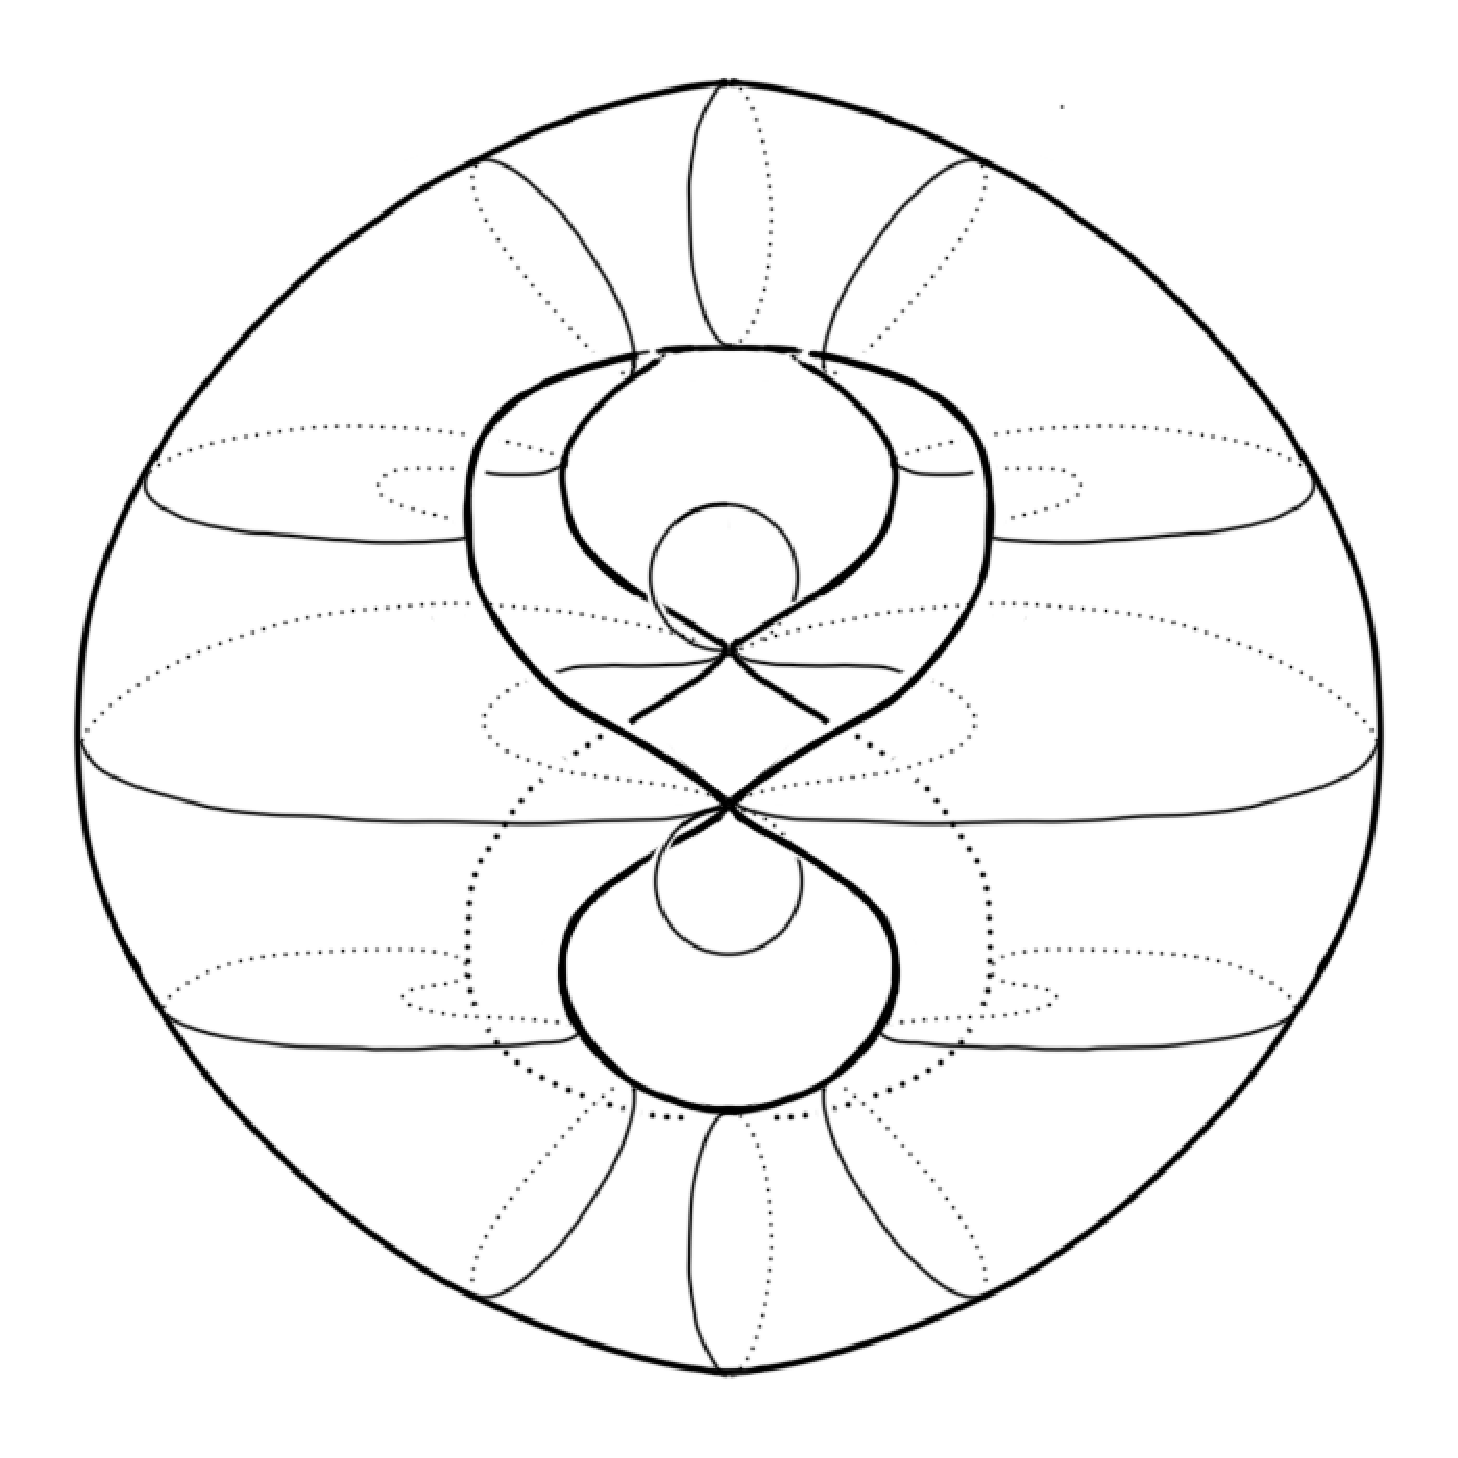
\includegraphics[width=6cm]{images/ch4/section2/atoms/atom_8.pdf}
    \caption{Поверхность уровня $\Xi = \const$ для случая 8.}
    \label{fig:pt9:_atom_8}
\endminipage\hfill
\end{figure}


\textbf{Перестройка 9.}
Звенья траектории в области $\Omega_{out}$ лежат на касательных к гиперболе с параметром $\alpha_{out}$, а в области $\Omega_{in}$ совпадают с вертикальной полуосью эллипса.

Поверхность $\Xi = \const$ можно представить себе как предельный случай неособой поверхности, соответствующей случаю $D_1^3$, при $\alpha_{in} \to a^2$ (см. рис. \ref{fig:pt9:_diagramPlusIrregular}), когда две ручки схлопываются в окружность.

Напомним рассуждения случая $D_1^3$. Рассмотрим склейку областей  $\widetilde{\Omega}_1$ (см. рис. \ref{fig:pt9:_img18}) и $\widetilde{\Omega}_4$  по общим границам, которые проецируются в эллиптические граничные дуги области $\widetilde{\Omega}$ и аналогичную склейку для областей $\widetilde{\Omega}_2$ и $\widetilde{\Omega}_3$.
Результатом склейки является сфера с шестью дырками, при этом каждая дырка ограничивается парой дуг на поверхности $\Xi=\const$, которые проецируются в граничные гиперболические дуги области $\widetilde{\Omega}$. 

Части границ областей $\widetilde{\Omega}_1$ и $\widetilde{\Omega}_2$ отождествляются по дугам, которые проектируются в гиперболические дуги области $\widetilde{\Omega}$, аналогично для областей $\widetilde{\Omega}_3$ и $\widetilde{\Omega}_4$.

На рис. \ref{fig:pt9:_atom_9_step} изображен результат склейки $\widetilde{\Omega}_1 \cup \widetilde{\Omega}_4$. Границей этой поверхности являются три пары окружностей, по которым приклеивается поверхность, полученная в результате аналогичной  склейки  $\widetilde{\Omega}_2 \cup \widetilde{\Omega}_3$. 

В момент перестройки две граничные окружности $\widetilde{\Omega}_1 \cup \widetilde{\Omega}_4$, которые проецируются в область $\Omega_{in}$, стягиваются в одну окружность.

Таким образом, поверхность $\Xi = \const$ представляет собой два тора, на каждом из которых отождествлено по две точки. При этом точки, полученные в результате такого отождествления, соединены двумя дугами, см. рис. \ref{fig:pt9:_atom_9}.
%
%\begin{figure}[!htb]
%\minipage{0.33\textwidth}
%\centering
%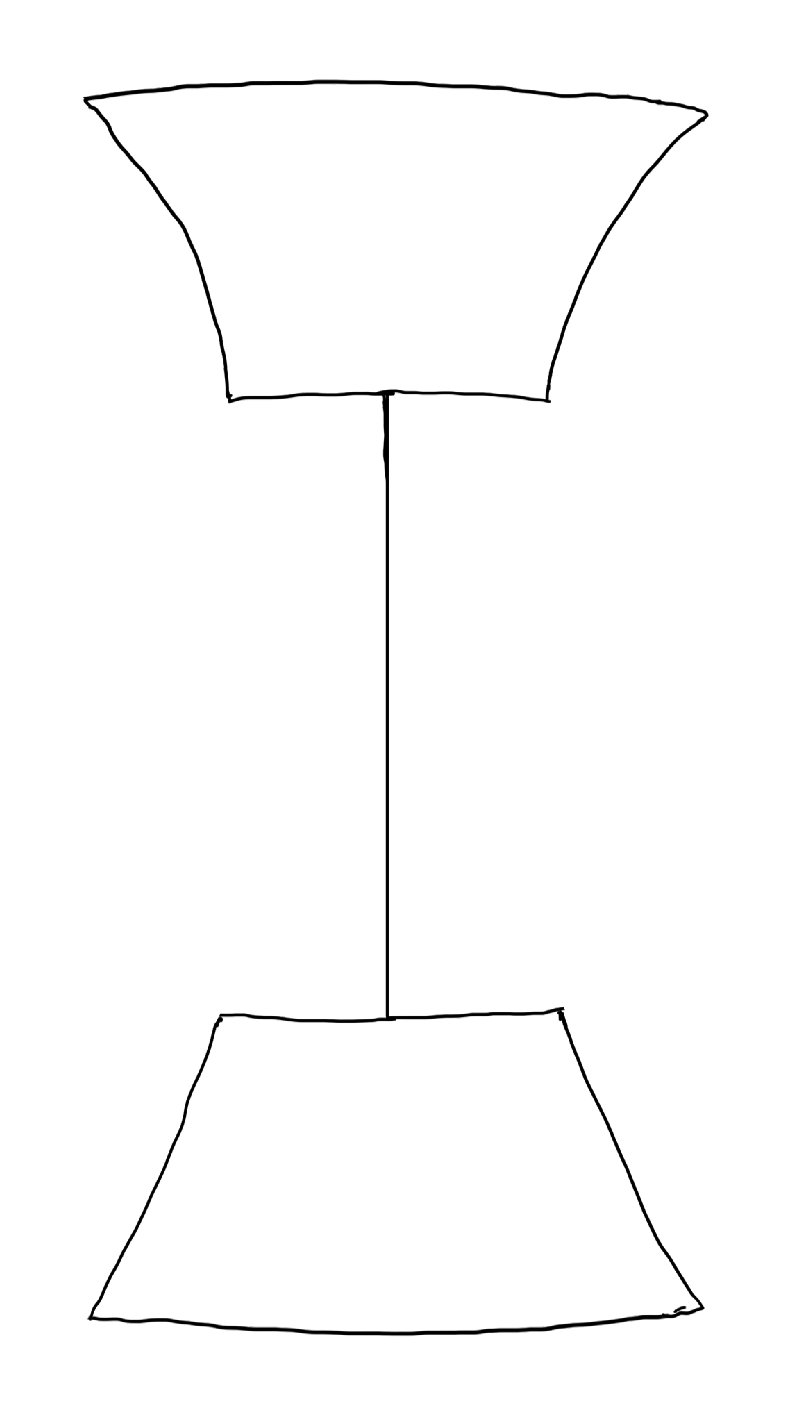
\includegraphics[scale=0.1]{images/ch4/section2/atoms/domain_atom_void_hyp.pdf}
%    \caption{Соответствующая случаю область $\Omega$.}
%    \label{fig:pt9:_domain_atom_void_hyp}
%\endminipage\hfill
%\minipage{0.32\textwidth}
%\centering
%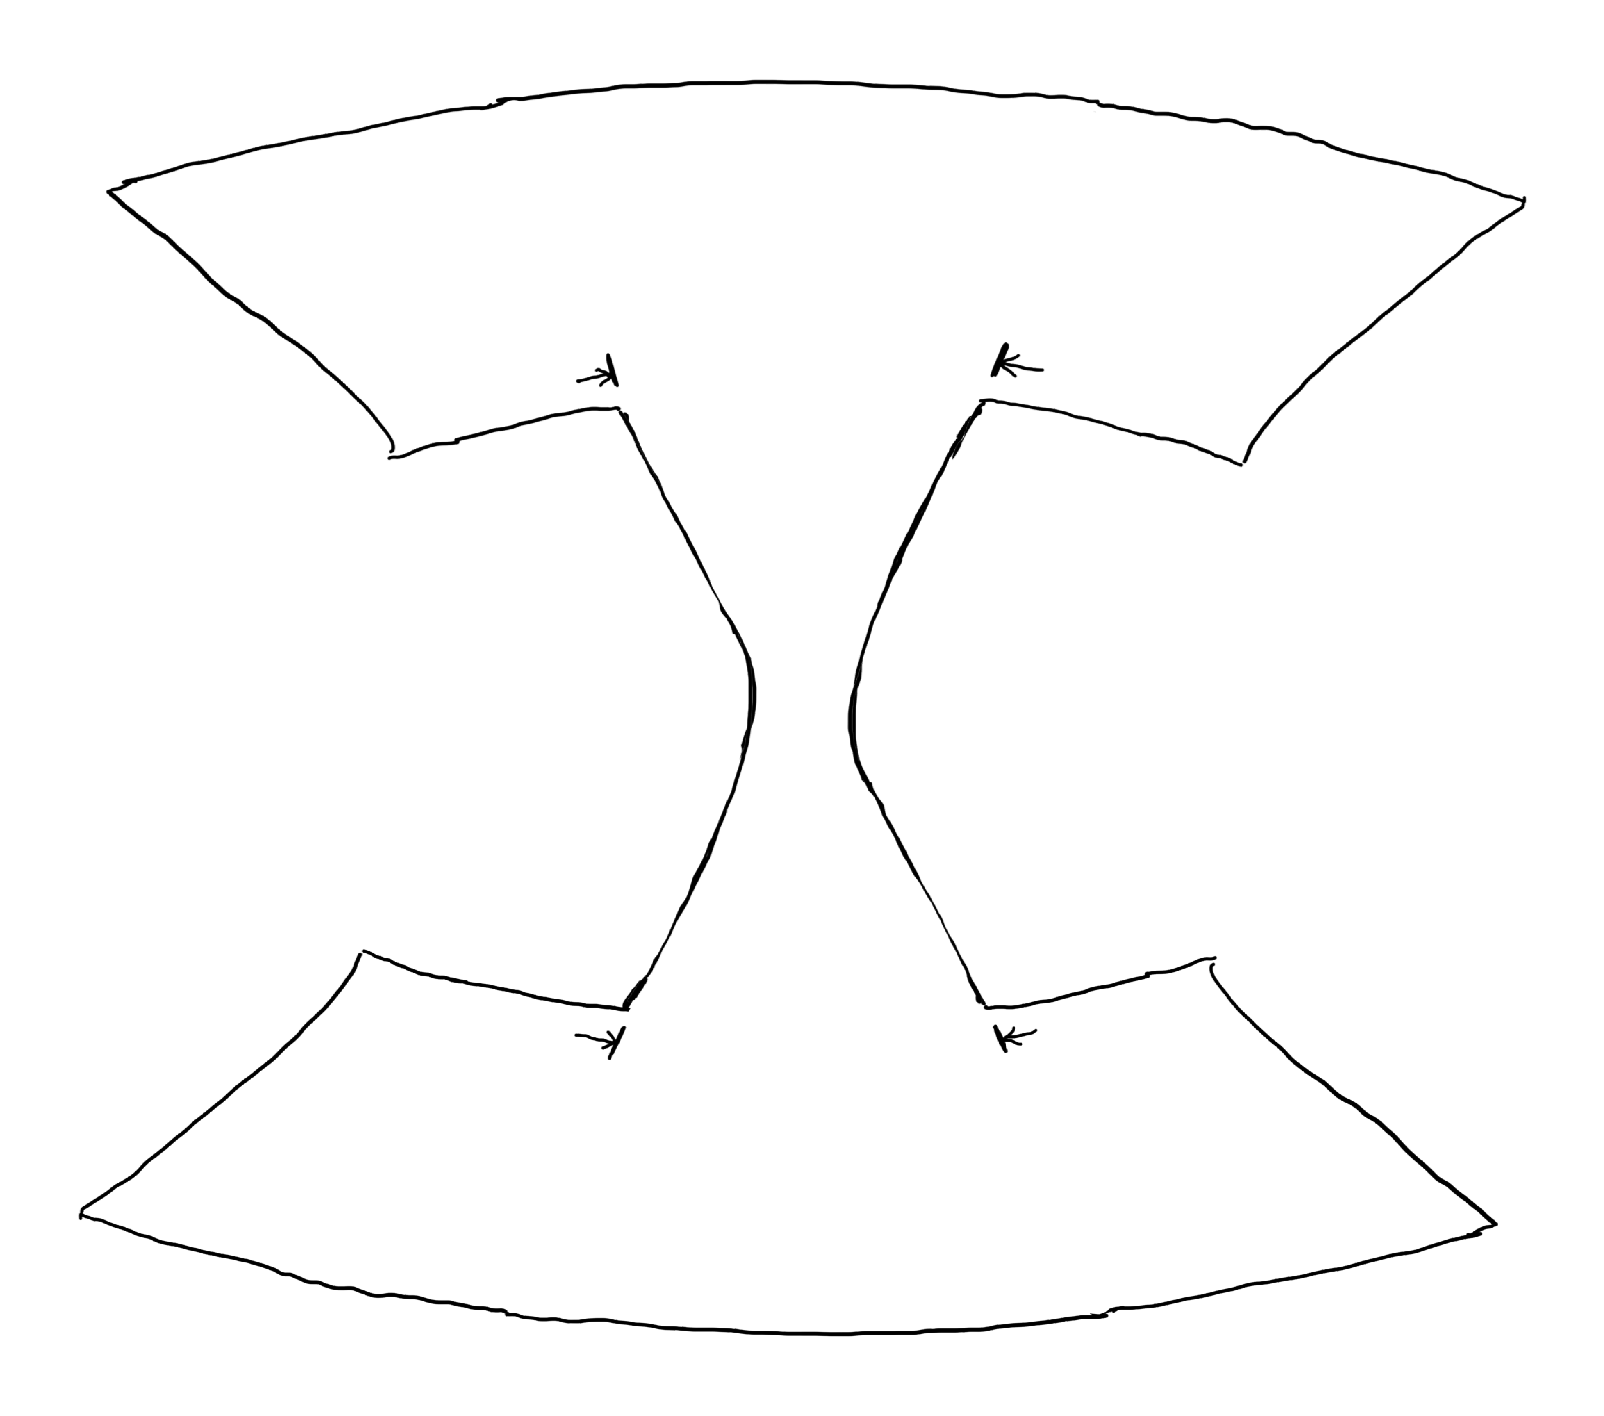
\includegraphics[scale=0.1]{images/ch4/section2/atoms/domain_atom_void_hyp_before_limit.pdf}
%    \caption{Область $\Omega$ как предельный случай.}
%    \label{fig:pt9:_domain_atom_void_hyp_before_limit}
%\endminipage\hfill
%\minipage{0.3\textwidth}
%\centering
%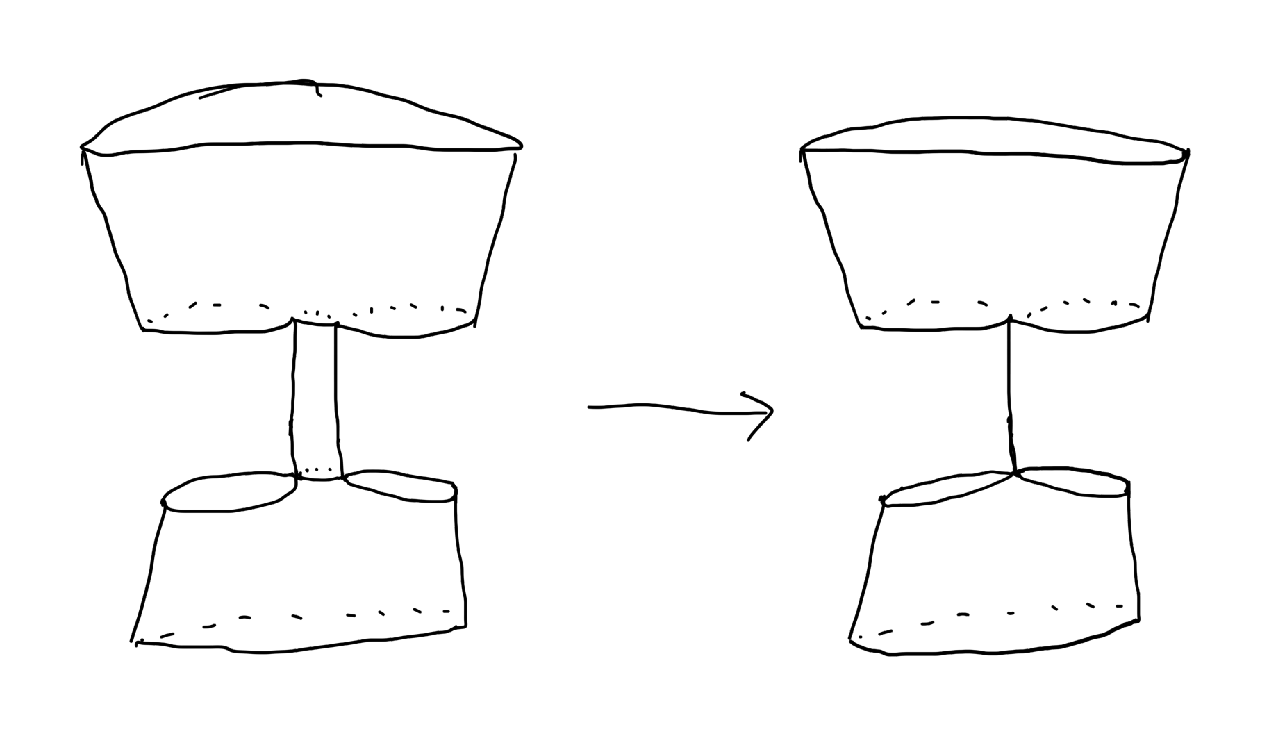
\includegraphics[scale=0.2]{images/ch4/section2/atoms/atom_void_hyp_iter1.pdf}
%    \caption{Схлопывание одной из ручек.}
%    \label{fig:pt9:_atom_void_hyp_iter1}
%\endminipage\hfill
%\end{figure}
%
%Для того, чтобы получить сам атом, остается провести склейку как показано на Рис. \ref{fig:pt9:_atom_void_hyp_iter2}, результат которой можно увидеть на Рис. \ref{fig:pt9:_void_hyp_atom}.

\begin{figure}[!htb]
\minipage{0.5\textwidth}
\centering
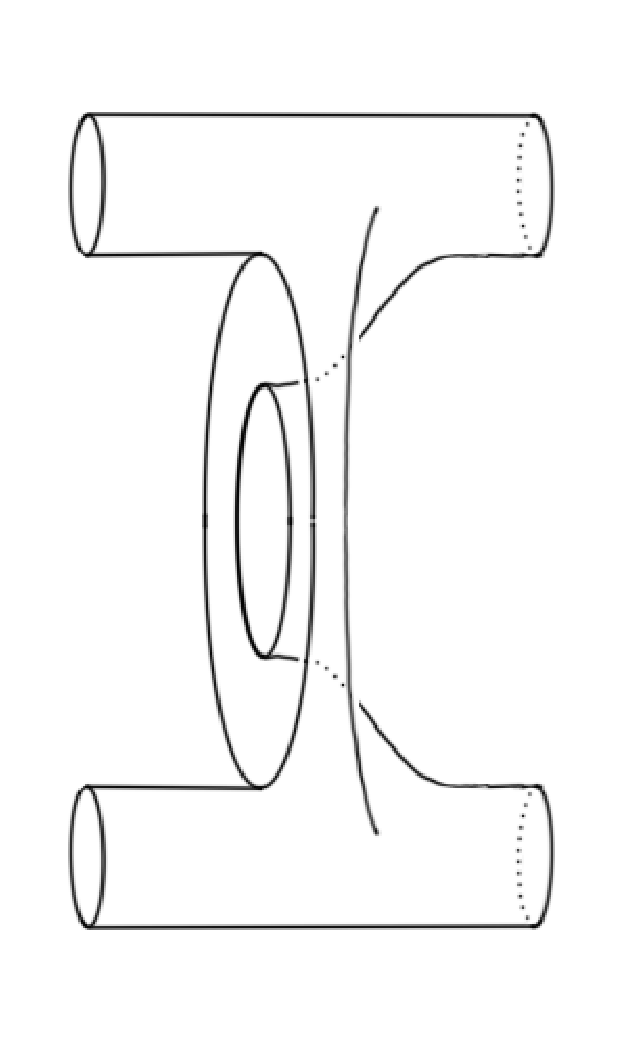
\includegraphics[width=2.5cm]{images/ch4/section2/atoms/atom_9_step.pdf}
\caption{Результат склейки $\widetilde{\Omega}_1 \cup \widetilde{\Omega}_4$ для перестройки 9.}
\label{fig:pt9:_atom_9_step}
\endminipage\hfill
\minipage{0.5\textwidth}
\centering
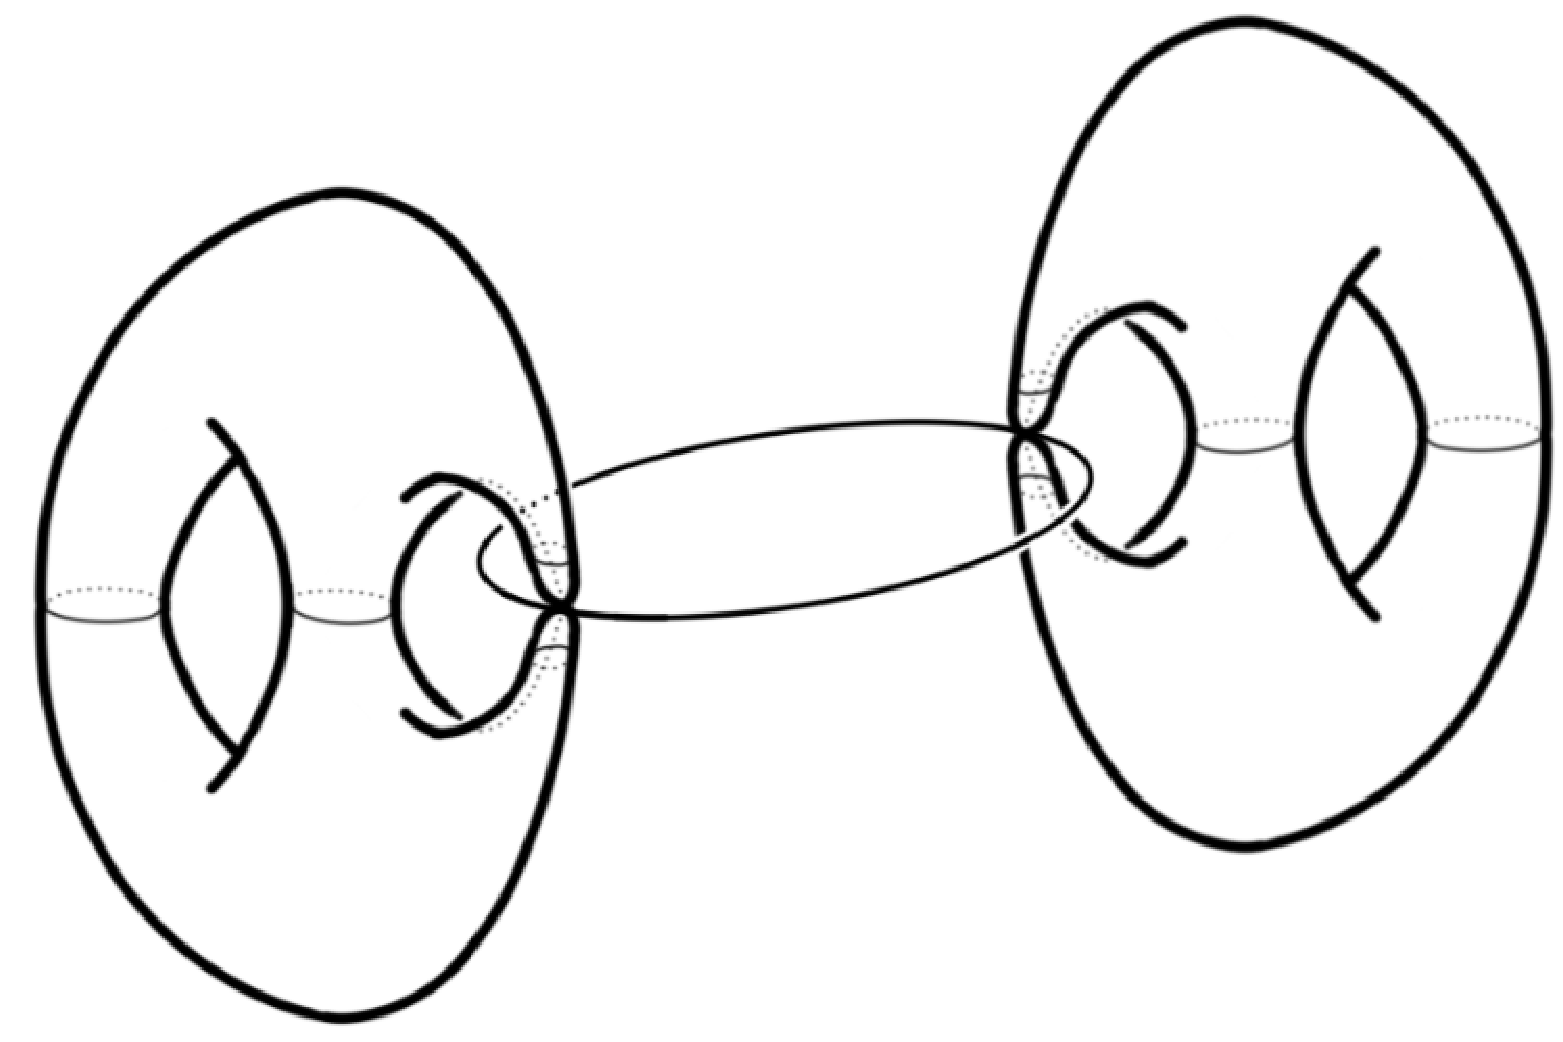
\includegraphics[width=5cm]{images/ch4/section2/atoms/atom_9.pdf}
\caption{Поверхность $\Xi = \const$ для случая 9.}
\label{fig:pt9:_atom_9}
\endminipage\hfill
\end{figure}

\textbf{Перестройка 10.}
Эта перестройка совпадает с перестройкой $\alpha_{out} \to b^2$ классического бильярда в эллиптическом кольце $\Omega_{out}$. Перестройка подробно разобрана в \cite[\S 3]{Fok15}.

\textbf{Перестройка 11.}
Как было отмечено выше, прямая \eqref{eq:L_line} проходит через точку $(\alpha_{in}, \alpha_{out}) = (\lambda_1, \lambda_1)$ и имеет коэффициент наклона $\dfrac{n_{in}^2}{n_{out}^2}$. 
Следовательно, такая перестройка возможна лишь в случае $n_{in}^2 = n_{out}^2$, что соответствует отсутствию преломления. Такая перестройка рассматривается в теории классического бильярда, см. \cite[\S 3]{Fok15}.

\textbf{Перестройка 12.}
Звенья траектории в области $\Omega_{in}$ лежат на проходящих через фокусы прямых, а в области $\Omega_{out}$ совпадают с вертикальной полуосью эллипса. 

Поверхность $\Xi = \const$ можно представить себе как комбинацию перестроек $\textbf{4}$ и $\textbf{8}$ (или перестроек $\textbf{3}$ и $\textbf{7}$). 

Определим области $\widetilde{\Omega}_1, \ldots, \widetilde{\Omega}_4$, как в \eqref{fig:pt9:_atom_4_domain} (пример области см. рис. \ref{fig:pt9:_atom_4_domain}).
Склеим листы $\widetilde{\Omega}_1$ и  $\widetilde{\Omega}_4$ так же, как указано в \textbf{перестройке 4}. В момент перестройки граничные окружности должны схлопнуться в одну окружность. Поэтому те части склейки, которые проецируются в кольцо $\Omega_{out}$, продеформируем так же, как в \textbf{перестройке 8} (результат склейки см. рис. \ref{fig:pt9:_atom_12_half}).

Таким образом, поверхность $\Xi = \const$ представляет собой тор с восьмеркой в сечении, на котором отмечены  две пары отождествленных точек, принадлежащих разным <<компонентам>> восьмерок. При этом из точек, полученных в результате отождествления, <<растет>> по одной окружности, см. рис. \ref{fig:pt9:_atom_12}.


\begin{figure}[!htb]
\minipage{0.5\textwidth}
\centering
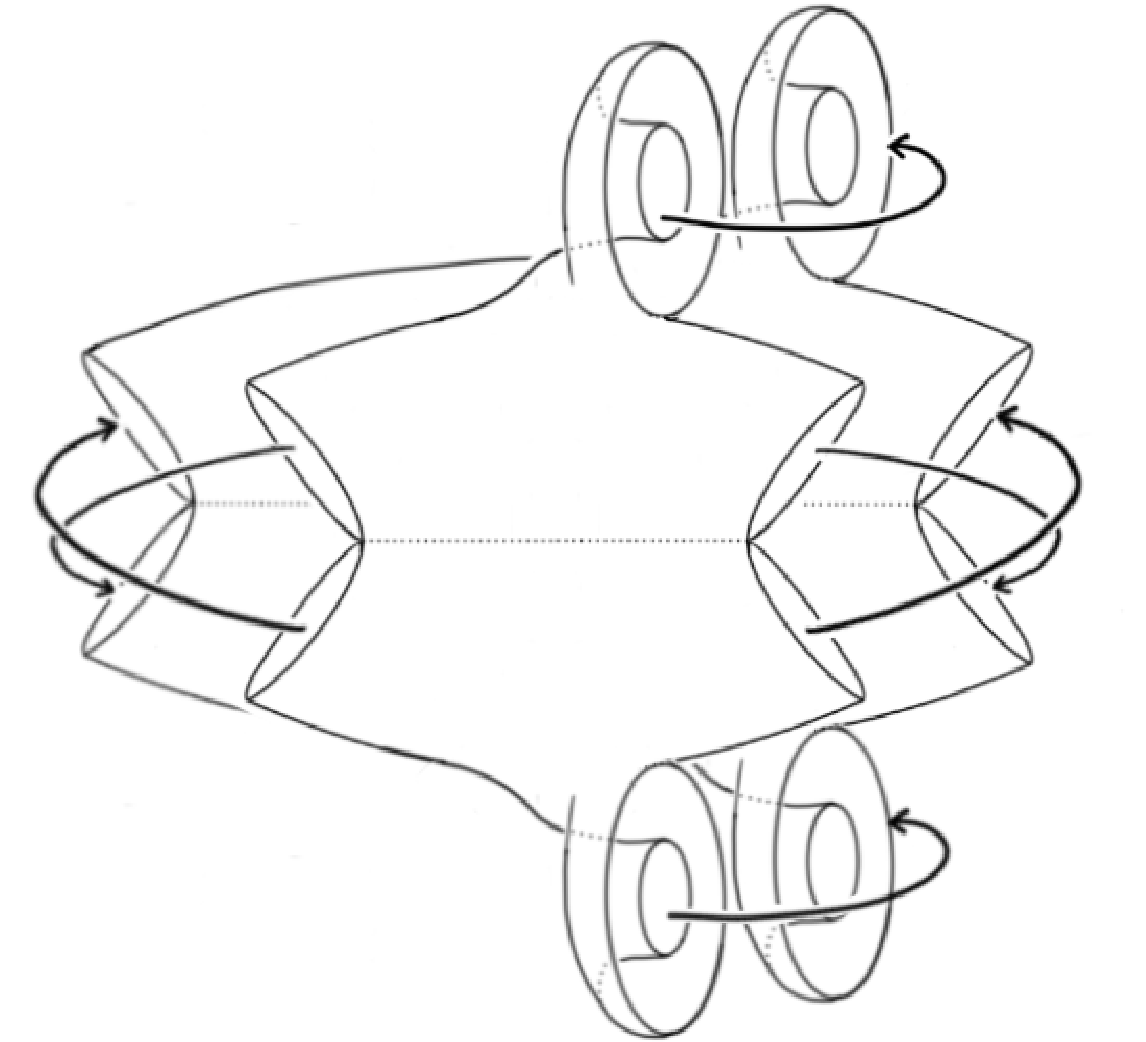
\includegraphics[scale=0.3]{images/ch4/section2/atoms/atom_12_half.pdf}
    \caption{Схема склейки $\Omega_1 \cup \Omega_4$ и $\Omega_2 \cup \Omega_3$ для случая 12.}
    \label{fig:pt9:_atom_12_half}
\endminipage\hfill
\minipage{0.5\textwidth}
\centering
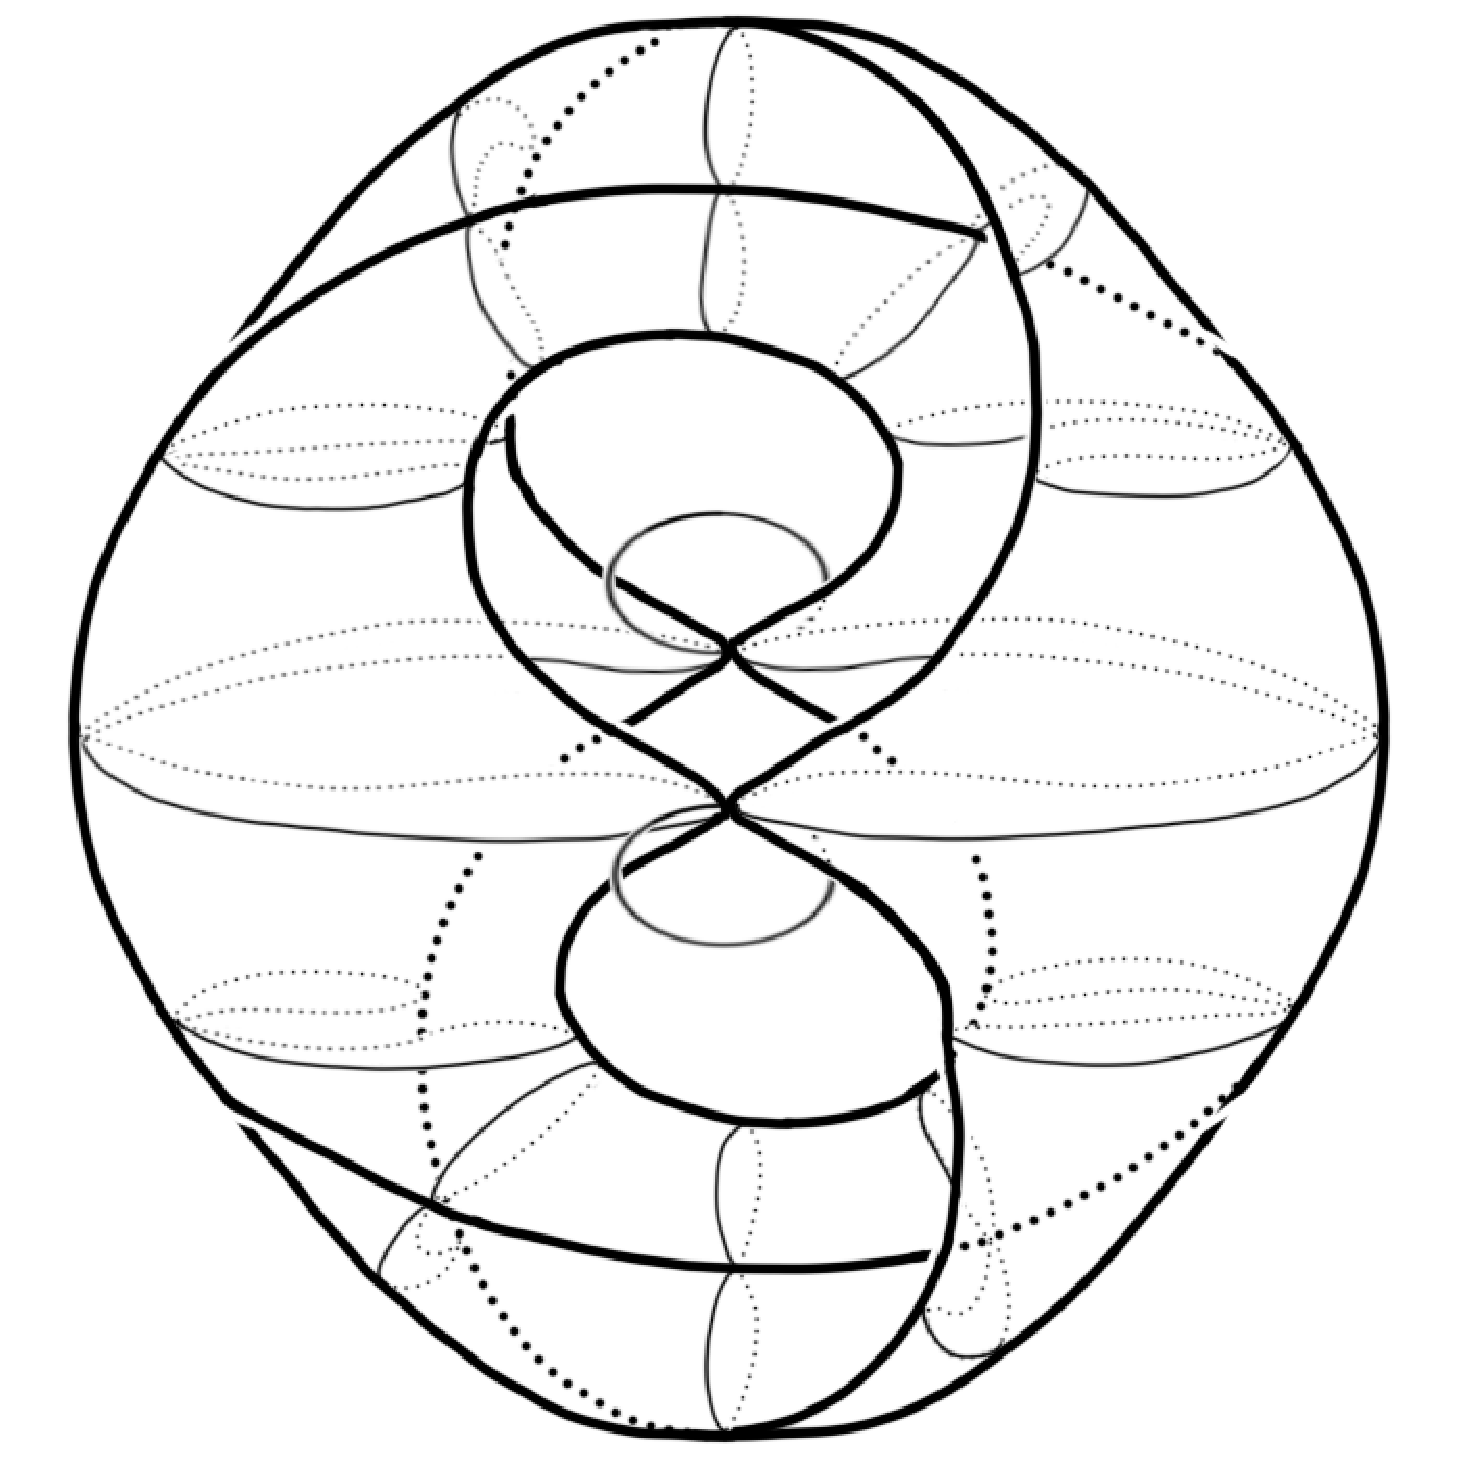
\includegraphics[scale=0.2]{images/ch4/section2/atoms/atom_12.pdf}
    \caption{Поверхность уровня $\Xi = \const$ для случая 12.}
    \label{fig:pt9:_atom_12}
\endminipage\hfill
\end{figure}



\textbf{Перестройка 13.}
Звенья траектории в области $\Omega_{out}$ лежат на проходящих через фокусы прямых, а в области $\Omega_{in}$ совпадают с вертикальной полуосью эллипса.

Поверхность $\Xi = \const$ можно представить себе как комбинацию перестроек $\textbf{5}$ и $\textbf{9}$ (или перестроек $\textbf{6}$ и $\textbf{10}$).

Определим области $\widetilde{\Omega}_1, \ldots, \widetilde{\Omega}_4$, как в \eqref{eq:case5Omegas} (пример области см. рис. \ref{fig:pt9:_domain_atom_hyp_foc}).
Склеим листы $\widetilde{\Omega}_1$ и  $\widetilde{\Omega}_4$ так же, как указано в \textbf{перестройке 5}. В момент перестройки две трубки, образованные проецирующимися в $\Omega_{in}$ частями листов, должны схлопнуться в одну окружность. Отождествим полученную поверхность вдоль дуг $\delta_1, \ldots, \delta_4$, результат склейки изображен на  рис. \ref{fig:pt9:_atom_13_half}.

Поверхность $\Xi = \const$ получается склейкой поверхности по граничным окружностям, результат изображен на рис. \ref{fig:pt9:_atom_13}.

\begin{figure}[!htb]
\minipage{0.5\textwidth}
\centering
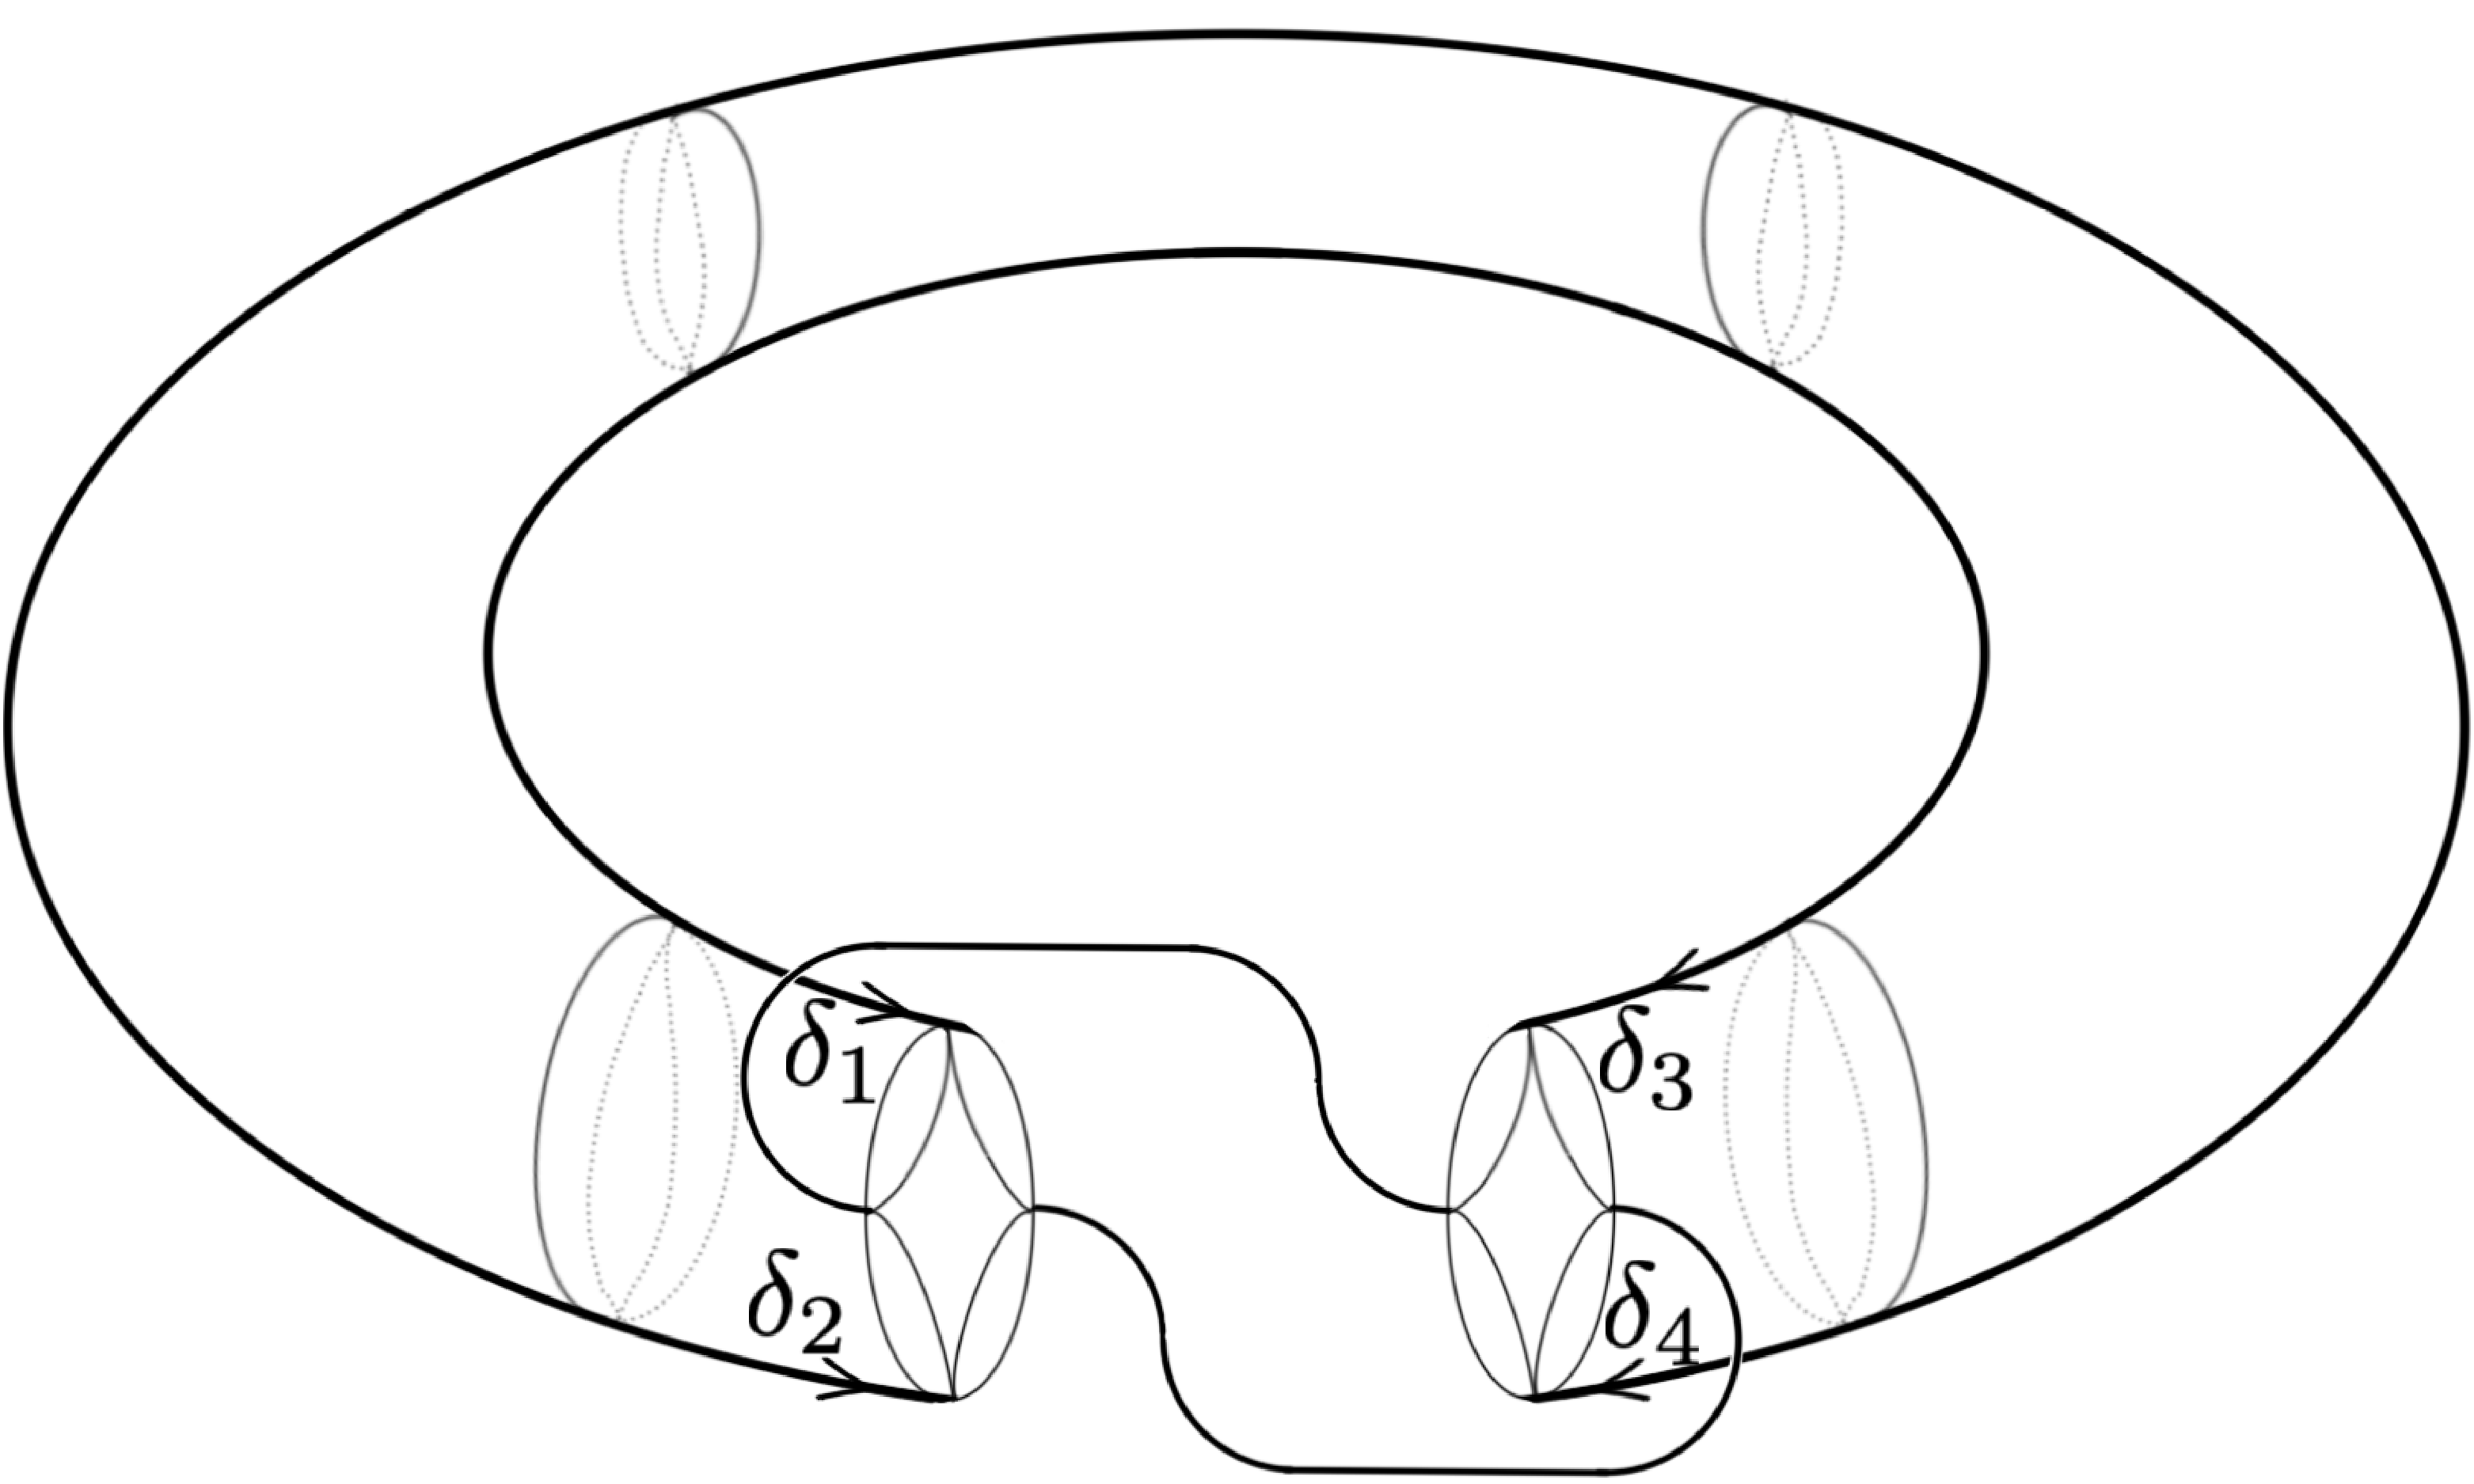
\includegraphics[scale=0.1]{images/ch4/section2/atoms/atom_13_half.pdf}
    \caption{Схема склейки $\Omega_1 \cup \Omega_2$ и $\Omega_3 \cup \Omega_4$ для случая 13.}
    \label{fig:pt9:_atom_13_half}
\endminipage\hfill
\minipage{0.5\textwidth}
\centering
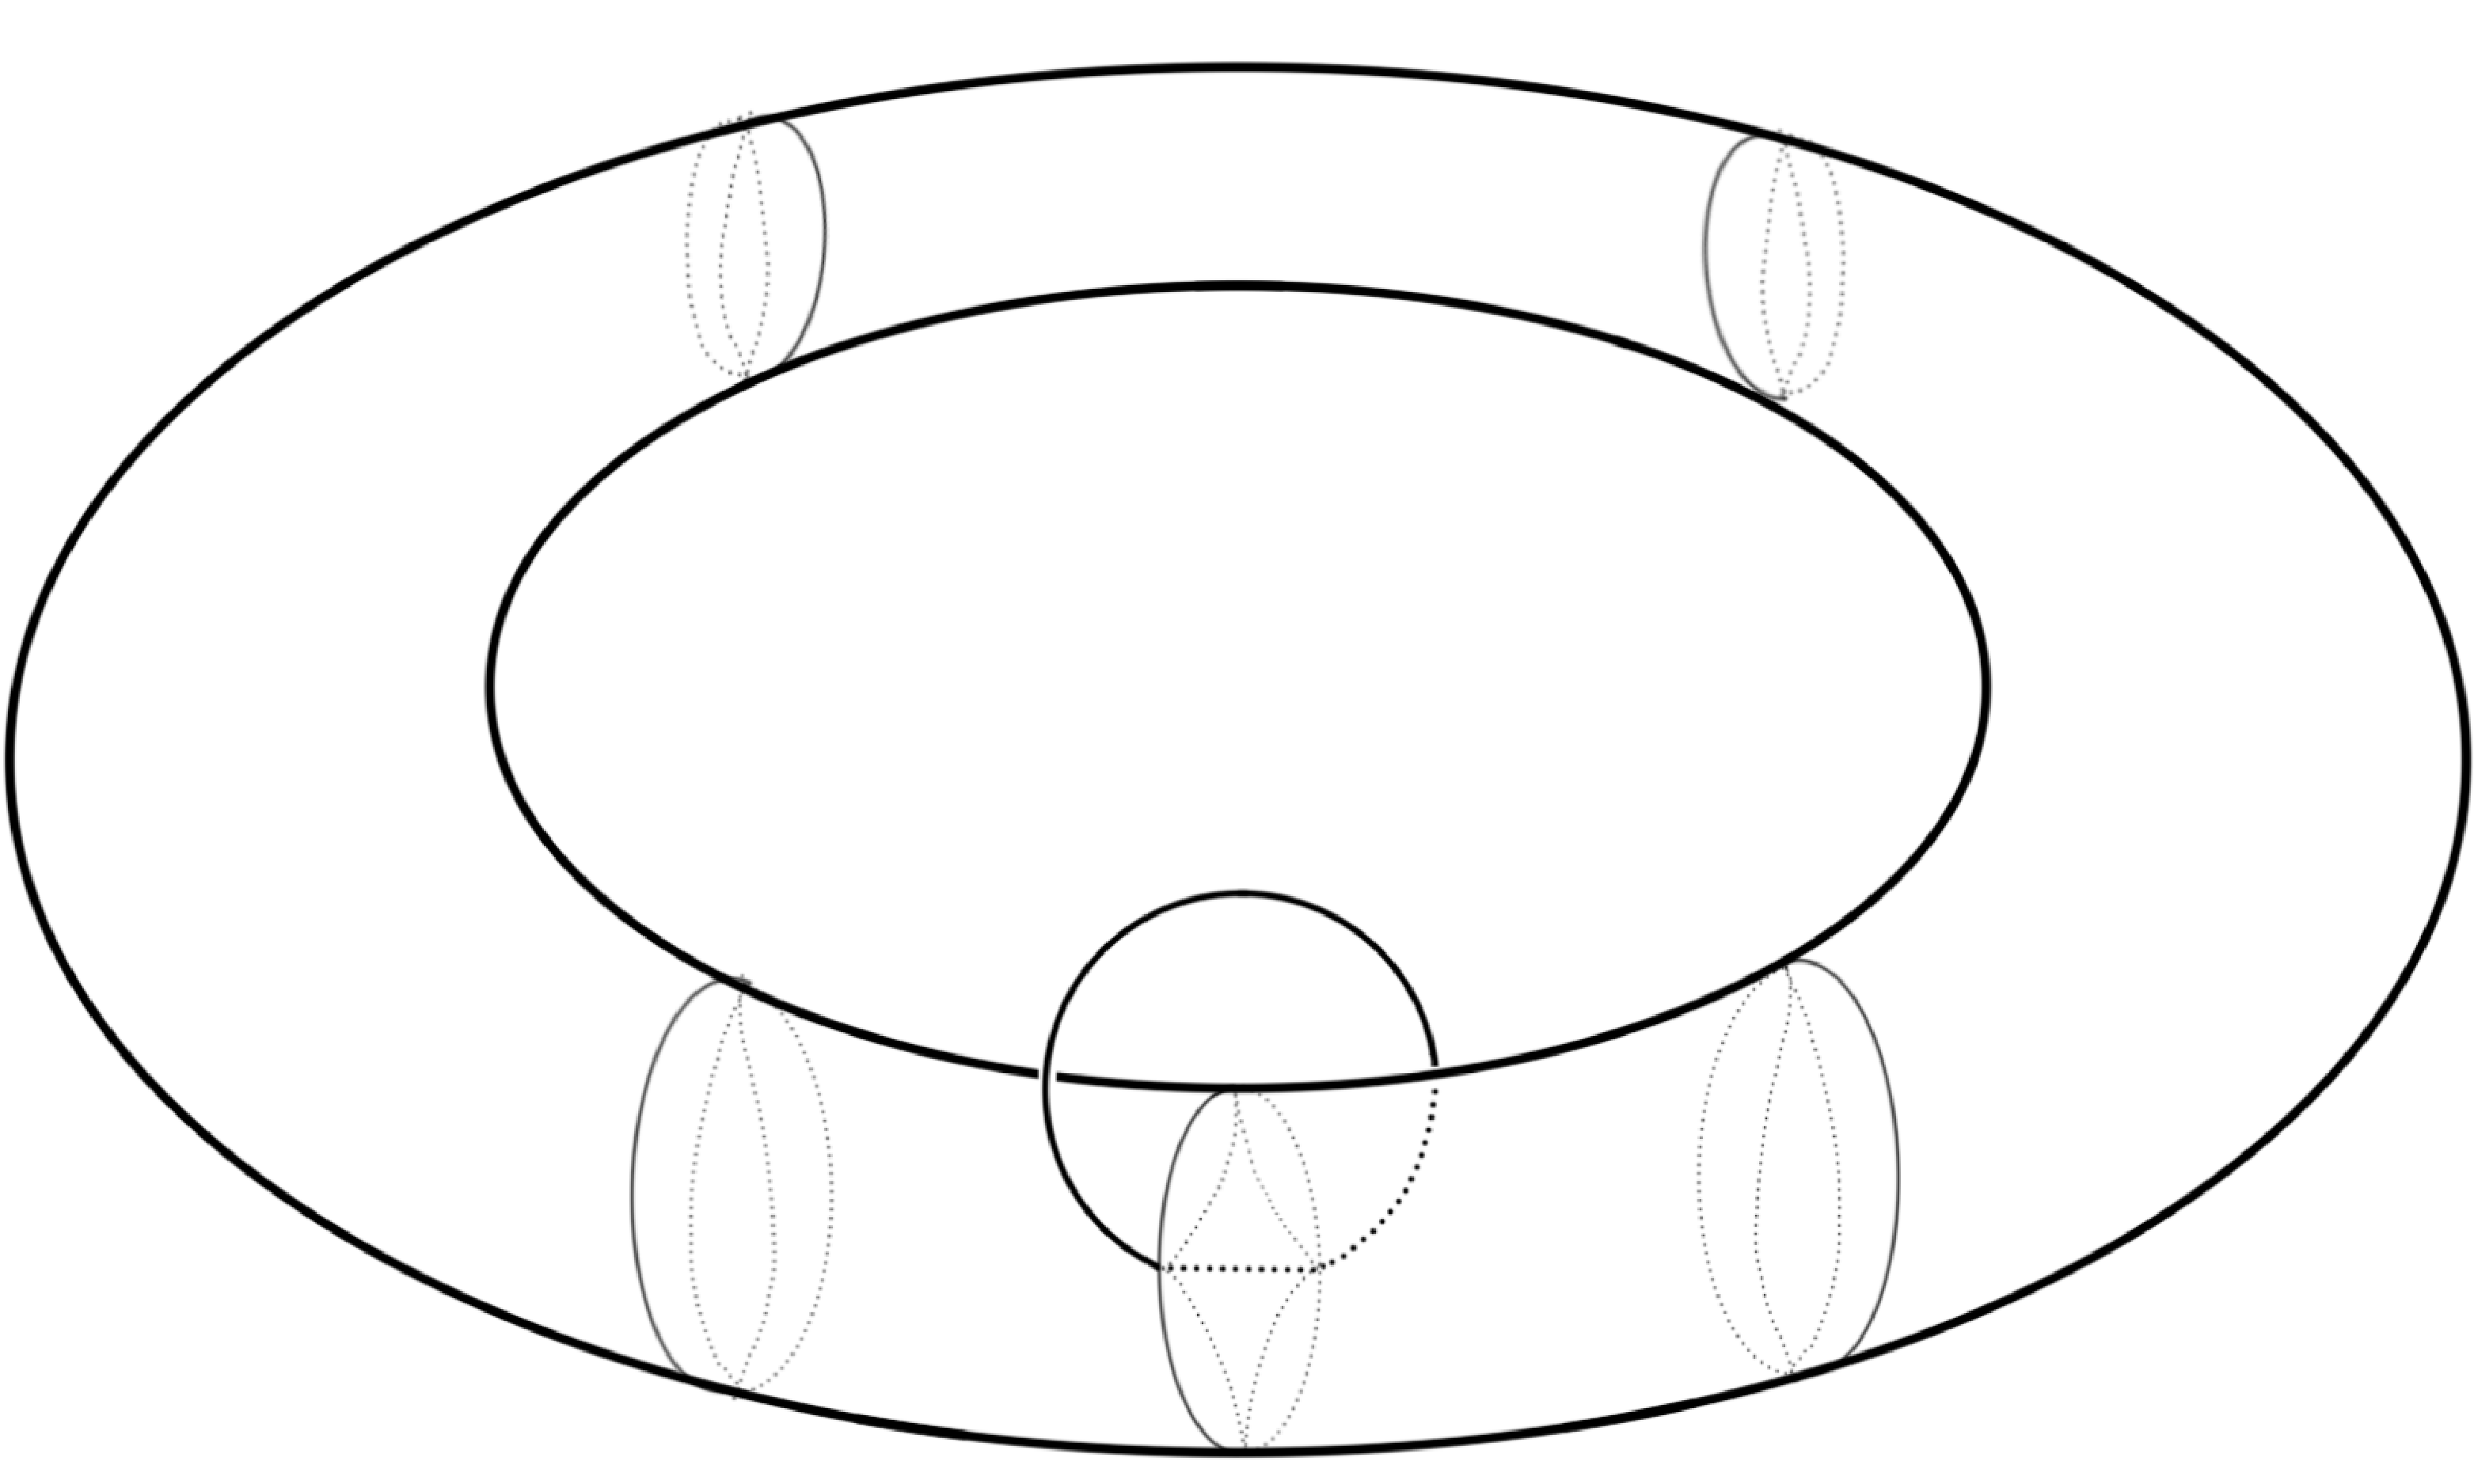
\includegraphics[scale=0.1]{images/ch4/section2/atoms/atom_13.pdf}
    \caption{Поверхность уровня $\Xi = \const$ для случая 13.}
    \label{fig:pt9:_atom_13}
\endminipage\hfill
\end{figure}

